\documentclass{cmspaper}
\usepackage{graphicx}
\usepackage{amsmath}
\usepackage{amssymb}
\usepackage{subfigure}
\usepackage{multirow}
\usepackage[pdfborder=0 0 0,
            colorlinks,
            urlcolor = blue,
            linkcolor = black,
            citecolor = black,
            menucolor = black,]
           {hyperref}
%% \usepackage[colorlinks]{hyperref}
%% \usepackage{url}
\usepackage[toc,page]{appendix}
\usepackage{varioref}
\renewcommand{\appendixname}{Appendix}
%% \renewcommand{\appendixtocname}{List of appendices}

% % useful definitions

% processes
\def\dyee {\ensuremath{Z/\gamma^*\to ee}}
\def\dymm {\ensuremath{Z/\gamma^*\to\mu\mu}}
\def\dytt {\ensuremath{Z/\gamma^*\to\tau\tau}}
\def\zee {\ensuremath{Z\to ee}}
\def\zmm {\ensuremath{Z\to\mu\mu}}
\def\ztt {\ensuremath{Z\to\tau\tau}}
\def\ttbar {\ensuremath{t\bar{t}}}
\def\wwll {\ensuremath{WW\to l^+l^-}}
\def\wwlulu{\ensuremath{WW\to l^+\nu l^-\bar{\nu}}}
\def\ww {\ensuremath{WW}}
\def\hww {\ensuremath{H\to WW}}
\def\wz{\ensuremath{WZ}}
\def\zz{\ensuremath{ZZ}}
\def\wgamma{\ensuremath{W\gamma}}
\def\wjets{\ensuremath{W+}jets} 
\def\tw{\ensuremath{tW}} 
\def\singletopt{\ensuremath{t} ($t$-chan)} 
\def\singletops{\ensuremath{t} ($s$-chan)} 
\def\all{all}
\def\ee{\ensuremath{ee}}
\def\emu{\ensuremath{e\mu}}
\def\mm{\ensuremath{\mu\mu}}

%units
\newcommand{\TeV}{\ensuremath{\mathrm{Te\kern -0.1em V}}}
\newcommand{\GeV}{\ensuremath{\mathrm{Ge\kern -0.1em V}}}

%others
\def\pt{\ensuremath{p_T}}
\def\ipb{pb\ensuremath{^{-1}}}
\def\ifb{fb\ensuremath{^{-1}}}
\def\et{\ensuremath{E_T}}
\def\met{\ensuremath{E\!\!\!\!/_T}}
\def\fBrem{\ensuremath{f_{\rm brem}}}
\def\pin{\ensuremath{p_{\rm in}}}
\def\pout{\ensuremath{p_{\rm out}}}

\newcommand{\CLs}{\ensuremath{CL_\mathrm{s}}}
\newcommand{\CLb}{\ensuremath{CL_\mathrm{b}}}
\newcommand{\CLsb}{\ensuremath{CL_\mathrm{s+b}}}

\newcommand{\GeV}{\ensuremath{\mathrm{Ge\kern -0.1em V}}}
\newcommand{\TeV}{\ensuremath{\mathrm{Te\kern -0.1em V}}}
\newcommand{\TeVcc}{\ensuremath{\,\mathrm{Te\kern -0.1em V\!/c}^2}}
\newcommand{\GeVcc}{\ensuremath{\,\mathrm{Ge\kern -0.1em V\!/c}^2}}
\newcommand{\MeVcc}{\ensuremath{\,\mathrm{Me\kern -0.1em V\!/c}^2}}
\newcommand{\GeVc}{\ensuremath{\mathrm{Ge\kern -0.1em V}\!/c}}
\newcommand{\nanob}{\mbox{{\rm ~nb}~}}
\newcommand{\fb}{\ensuremath{\mathrm{fb}}}
\newcommand{\pb}{\ensuremath{\mathrm{pb}}}
\newcommand{\ifb}{\ensuremath{\mathrm{fb^{-1}}}}
\newcommand{\ipb}{\ensuremath{\mathrm{pb^{-1}}}}
\newcommand{\grad}{\ensuremath{^{\circ}}}
%
% Special user made math symbols
%
\newcommand{\lsim}{\raisebox{-1.5mm}{$\:\stackrel{\textstyle{<}}{\textstyle{\sim}}\:$}}
\newcommand{\gsim}{\raisebox{-1.5mm}{$\:\stackrel{\textstyle{>}}{\textstyle{\sim}}\:$}}

% particles

\newcommand{\pipm}{\ensuremath{\pi^{\pm}}}
\newcommand{\pizero}{\ensuremath{\pi^{0}}}
\newcommand{\Hi}{\ensuremath{\mathrm{H}}}
\newcommand{\W}{\ensuremath{\mathrm{W}}}
\newcommand{\Wjets}{\ensuremath{\mathrm{W+jets}}}
\newcommand{\Zjets}{\ensuremath{\mathrm{Z+jets}}}
\newcommand{\Wt}{\ensuremath{\mathrm{Wt}}}
\newcommand{\Wstar}{\ensuremath{\mathrm{W}^{*}}}
\newcommand{\Wparenthesisstar}{\ensuremath{\mathrm{W}^{(*)}}}
\newcommand{\WW}{\ensuremath{\W^+\W^-}}
\newcommand{\Z}{\ensuremath{\mathrm{Z}}}
\newcommand{\Zstar}{\ensuremath{\mathrm{Z}^{*}}}
\newcommand{\Astar}{\ensuremath{\mathrm{\gamma}^{*}}}
\newcommand{\ZZ}{\ensuremath{\Z\Z}}
\newcommand{\WZ}{\ensuremath{\W\Z}}
\newcommand{\Wgstar}{\ensuremath{\W\Astar}}
\newcommand{\E}{\ensuremath{\mathrm{e}}}
\newcommand{\Ep}{\ensuremath{\mathrm{e}^{+}}}
\newcommand{\Em}{\ensuremath{\mathrm{e}^{-}}}
\newcommand{\Epm}{\ensuremath{\mathrm{e}^{\pm}}}
\newcommand{\Emp}{\ensuremath{\mathrm{e}^{\mp}}}
\newcommand{\M}{\ensuremath{\mu}}
\newcommand{\Mp}{\ensuremath{\mu^{+}}}
\newcommand{\Mm}{\ensuremath{\mu^{-}}}
\newcommand{\Mpm}{\ensuremath{\mu^{\pm}}}
\newcommand{\Mmp}{\ensuremath{\mu^{\mp}}}
\newcommand{\Tau}{\ensuremath{\tau}}
\newcommand{\Nu}{\ensuremath{\nu}}
\newcommand{\Nubar}{\ensuremath{\bar{\nu}}}
\newcommand{\Lep}{\ensuremath{\ell}}
\newcommand{\Lepp}{\ensuremath{\ell^{+}}}
\newcommand{\Lepm}{\ensuremath{\ell^{-}}}
\newcommand{\Lprime}{\ensuremath{\Lep^{\prime}}}
\newcommand{\Prot}{\ensuremath{\mathrm{p}}}
\newcommand{\Pbar}{\ensuremath{\bar{\mathrm{p}}}}
\newcommand{\PP}{\Prot\Prot}
\newcommand{\PPbar}{\Prot\Pbar}
\newcommand{\ttbar}{\ensuremath{\mathrm{t}\bar{\mathrm{t}}}}
\newcommand{\qq}{\ensuremath{\mathrm{q}\mathrm{q}}}
%\newcommand{\bbbar}{\ensuremath{\mathrm{b}\bar{\mathrm{b}}}}
\newcommand{\Wtb}{\ensuremath{\W\mathrm{t}\mathrm{b}}}
\newcommand{\Top}{\ensuremath{\mathrm{t}}}
\newcommand{\Bot}{\ensuremath{\mathrm{b}}}
\newcommand{\Atop}{\ensuremath{\bar{\mathrm{t}}}}
\newcommand{\Abot}{\ensuremath{\bar{\mathrm{b}}}}
% arrow
\newcommand{\To}{\ensuremath{\rightarrow}}

% masses
\newcommand{\mHi}{\ensuremath{m_{\mathrm{H}}}}
\newcommand{\mW}{\ensuremath{m_{\mathrm{W}}}}
\newcommand{\mZ}{\ensuremath{m_{\mathrm{Z}}}}
\newcommand{\mll}{\ensuremath{m_{\Lep\Lep}}}
\newcommand{\mt}{\ensuremath{m_{\mathrm{T}}}}

% kinematics
\newcommand{\pt}{\ensuremath{p_\mathrm{T}}}
\newcommand{\ptveto}{\ensuremath{\pt^\mathrm{veto}}}
\newcommand{\ptl}{\ensuremath{p_\perp^{\Lep}}}
\newcommand{\ptlmax}{\ensuremath{p_{\mathrm{T}}^{\Lep,\mathrm{max}}}}
\newcommand{\ptlmin}{\ensuremath{p_{\mathrm{T}}^{\Lep,\mathrm{min}}}}
\newcommand{\met}{\ensuremath{\Et^{\mathrm{miss}}}}
\newcommand{\delphill}{\ensuremath{\Delta\phi_{\Lep\Lep}}}
\newcommand{\deletall}{\ensuremath{\Delta\eta_{\Lep\Lep}}}
\newcommand{\delphimetl}{\ensuremath{\Delta\phi_{\met\Lep}}}
\newcommand{\Et}{\ensuremath{E_\mathrm{T}}}
\newcommand{\delR}{\ensuremath{\Delta R}}
\newcommand{\Eta}{\ensuremath{\eta}}

%efficiencies
\newcommand{\effsig}{\ensuremath{\varepsilon_{\mathrm{bkg}}^{\mathrm{S}}}}
\newcommand{\effnorm}{\ensuremath{\varepsilon_{\mathrm{bkg}}^{\mathrm{N}}}}
\newcommand{\Nsig}{\ensuremath{N_{\mathrm{bkg}}^{\mathrm{S}}}}
\newcommand{\Nnorm}{\ensuremath{N_{\mathrm{bkg}}^{\mathrm{N}}}}

% processes
\newcommand{\dyee}{\ensuremath{Z/\gamma^*\to ee}}
\newcommand{\dymm}{\ensuremath{Z/\gamma^*\to\mu\mu}}
\newcommand{\dytt}{\ensuremath{Z/\gamma^*\to\tau\tau}}
\newcommand{\dyll}{\ensuremath{Z/\gamma^*\to\ell\ell}}
\newcommand{\dy}{\ensuremath{Z/\gamma^*}}
\newcommand{\zee}{\ensuremath{Z\to ee}}
\newcommand{\zmm}{\ensuremath{Z\to\mu\mu}}
\newcommand{\ztt}{\ensuremath{Z\to\tau\tau}}
%\newcommand{\ttbar}{\ensuremath{t\bar{t}}}
\newcommand{\ppww}{\ensuremath{pp \to W^+W^-}}
\newcommand{\wwll}{\ensuremath{WW\to \ell^+\ell^-}}
\newcommand{\wwlnln}{\ensuremath{W^+W^-\to \ell^+\nu \ell^-\bar{\nu}}}
\newcommand{\ww}{\ensuremath{WW}}
\newcommand{\wwpm}{\ensuremath{W^+W^-}}
\newcommand{\hww}{\ensuremath{H\to W^+W^-}}
\newcommand{\wz}{\ensuremath{WZ}}
\newcommand{\zz}{\ensuremath{ZZ}}
\newcommand{\wgamma}{\ensuremath{W\gamma}}
\newcommand{\wjets}{\ensuremath{W+}jets} 
\newcommand{\tw}{\ensuremath{tW}} 
\newcommand{\singletopt}{\ensuremath{t} ($t$-chan)} 
\newcommand{\singletops}{\ensuremath{t} ($s$-chan)} 
\newcommand{\zx}{\ensuremath{\mathrm{DY/WZ/ZZ}}}
\newcommand{\zv}{\ensuremath{\mathrm{WZ/ZZ}}}
\newcommand{\z}{\ensuremath{\mathrm{Z}}}
\newcommand{\routin}{\ensuremath{R_{out/in}}}

%other 
\def\fixme{({\bf FixMe})}
\newcommand{\ee}{\ensuremath{ee}}
\newcommand{\emu}{\ensuremath{e\mu}}
\def\mm{\ensuremath{\mu\mu}}

% integrated luminosity
\newcommand{\intlumiSevenTeV}{4.92~\ifb}
\newcommand{\intlumiEightTeV}{1.62~\ifb}

%%%%%%%%%%%
%
\newcounter{myfootertablecounter}

\newcommand\myfootnotemark{%
  %\refstepcounter{footnote}%
  \addtocounter{footnote}{1}%
  \footnotemark[\thefootnote]%
}%

\newcommand\myfootnotetext[1]{%
  \addtocounter{myfootertablecounter}{1}
  \footnotetext[\value{myfootertablecounter}]{#1}
}

% from now on, myfootnote has to be used rather than footnote to
% adapt the myfootercounter
\newcommand\myfootnote[1]{%
  \addtocounter{myfootertablecounter}{1}
  \footnote{#1}
}%



\setcounter{topnumber}{1}
\setcounter{bottomnumber}{1}
\setcounter{secnumdepth}{6}
%===================================================================================================
\begin{document}
\begin{titlepage}

  \analysisnote{2011/XXX}

  \date{\today}

  \title{A Higgs Boson Search in the Fully Leptonic $W^+W^-$ (update for ICHEP2012 conference)}

  \begin{Authlist}
%
L.~Bauerdick, K.~Burkett, I.~Fisk, Y.~Gao, O.~Gutsche, B.~Hooberman, S.~Jindariani, S.~Tkaczyk, V. Martinez Outschoorn, 
\Instfoot{fnal}{Fermilab National Accelerator Laboratory, Batavia, USA}
%
G.~Bauer, J.~Bendavid, E.~Butz, M.~Chan, V.~Dutta, G.~G\'omez-Ceballos, M.~Goncharov, K.~Hahn, P.~Harris, M.~Klute, S.~Nahn, C.~Paus, D.~Ralph, F.~Stoeckli, K.~Sumorok, K.~Sung, R.~Wolf, S.~Xie, M.~Yang, M.~Zanetti
\Instfoot{mit}{Laboratory for Nuclear Science, Massachusetts Institute of Technology, Cambridge, USA}
%
D.~Barge, C.~Campagnari, D.~Kovalskyi, V.~Krutelyov
\Instfoot{ucsb}{University of California, Santa Barbara, Santa Barbara, USA}
%
W.~Andrews, G.~Cerati, D.~Evans, F.~Golf, I.~MacNeill, S.~Padhi, Y.~Tu, F.~W\"urthwein, A.~Yagil, J.~Yoo
\Instfoot{ucsd}{University of California, San Diego, San Diego, USA}
%
I.~Kravchenko
\Instfoot{unl}{University of Nebraska-Lincoln, USA}

\end{Authlist}


  \begin{abstract}
    This note describes a search for the Higgs boson in the $W^+W^- \to
    2\ell2\nu$ final state with 0.82 $\ifb$ of $pp$ collision
    data at $\sqrt s = 8~\TeV$. We search for Higgs candidate 
    events in $ee$, $\mu\mu$ and $e\mu$ channels with 0, 1 and 2 
    reconstructed jets. We also measure the corresponding 
    $W^+W^-$ cross-section.
  \end{abstract} 

\end{titlepage}
\tableofcontents
%\listoftables
%\listoffigures
\newpage 

%===================================================================================================
\section{Introduction}
  \label{sec:overview}
  Precision measurement of the gauge boson couplings is a well known
method to look for physics beyond the Standard Model. In the case of
the triple gauge boson couplings, new physics contributions can be
expressed in the form of an effective Lagrangian. The most general
form of such a Lagrangian has 14 complex couplings (7 for $WWZ$ and 7 for
$WW\gamma$). Assuming electromagnetic gauge invariance, and C and P
symmetry conservation that number is reduced to five:
$\Delta\kappa_Z$, $\Delta g^Z_1$, $\Delta\kappa_{\gamma}$, $\lambda_Z$
and $\lambda_{\gamma}$. Applying gauge constraints:
\begin{align}
  \Delta\kappa_Z &= \Delta g^Z_1- \Delta\kappa_{\gamma}\tan^2\theta_W \\
  \lambda_Z &= \lambda_{\gamma}
\end{align}
further reduces the number of independent couplings to three. In the
Standard Model all five couplings are zero. 
 
CMS performed a first measurement of the anomalous couplings with
35/pb of data at 7 TeV~\cite{blah}. The measurement was performed with
and without a form factor that helps to avoid unitarity violation by
introducing an effective cutoff scale where a coupling is switched
off.  In this study we have two orders of magnitude more data and
experimental constraints on the couplings are more stringent then the
unitarity constraint. Therefore all the anomalous couplings are
form-factor free.

This analysis is based on the $W^+W^-$ production cross-section
measurement in $\intlumi$ of $pp$ collision data at $\sqrt{s} = $
7~$\TeV$ (the full 2011 dataset) \cite{ref:WWXS2011}. 

measurement~\cite{ref:WWXS2011}. Here we just briefly summarize the event
selection showing mostly kinematic requirements that may affect the
leading lepton pt distribution, which is used as a main observable.

The kinematic observable used in this analysis is 
the transverse momentum (\pt) of the leading lepton,
shown in Figure \ref{fig:pas_pt1_incl} after all event selections
have been applied.

\begin{figure}[hb]
\subfigure[Linear scale]{\label{subfig:pas_pt1_incl}
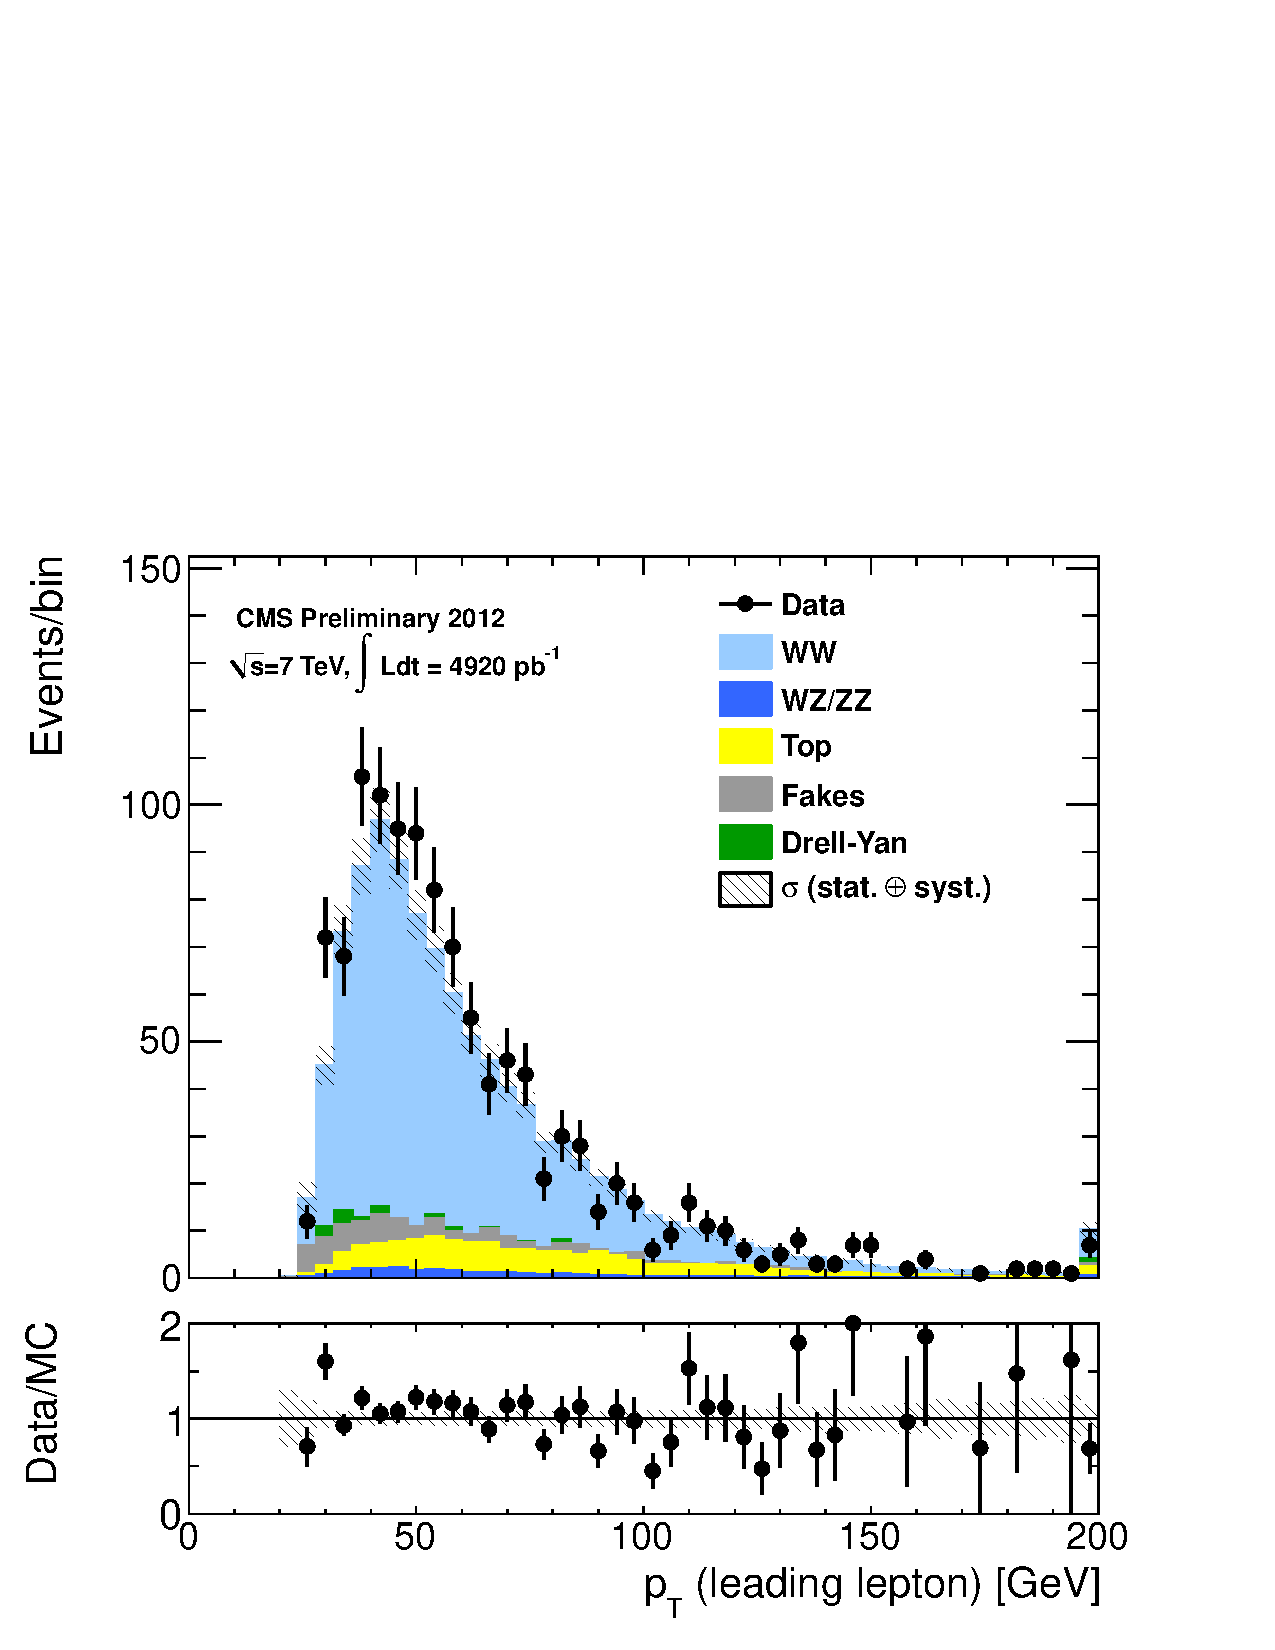
\includegraphics[width=.45\textwidth]{figures/pas_pt1_incl.pdf}}
\subfigure[Log scale]{\label{subfig:pas_pt1_incl_log}
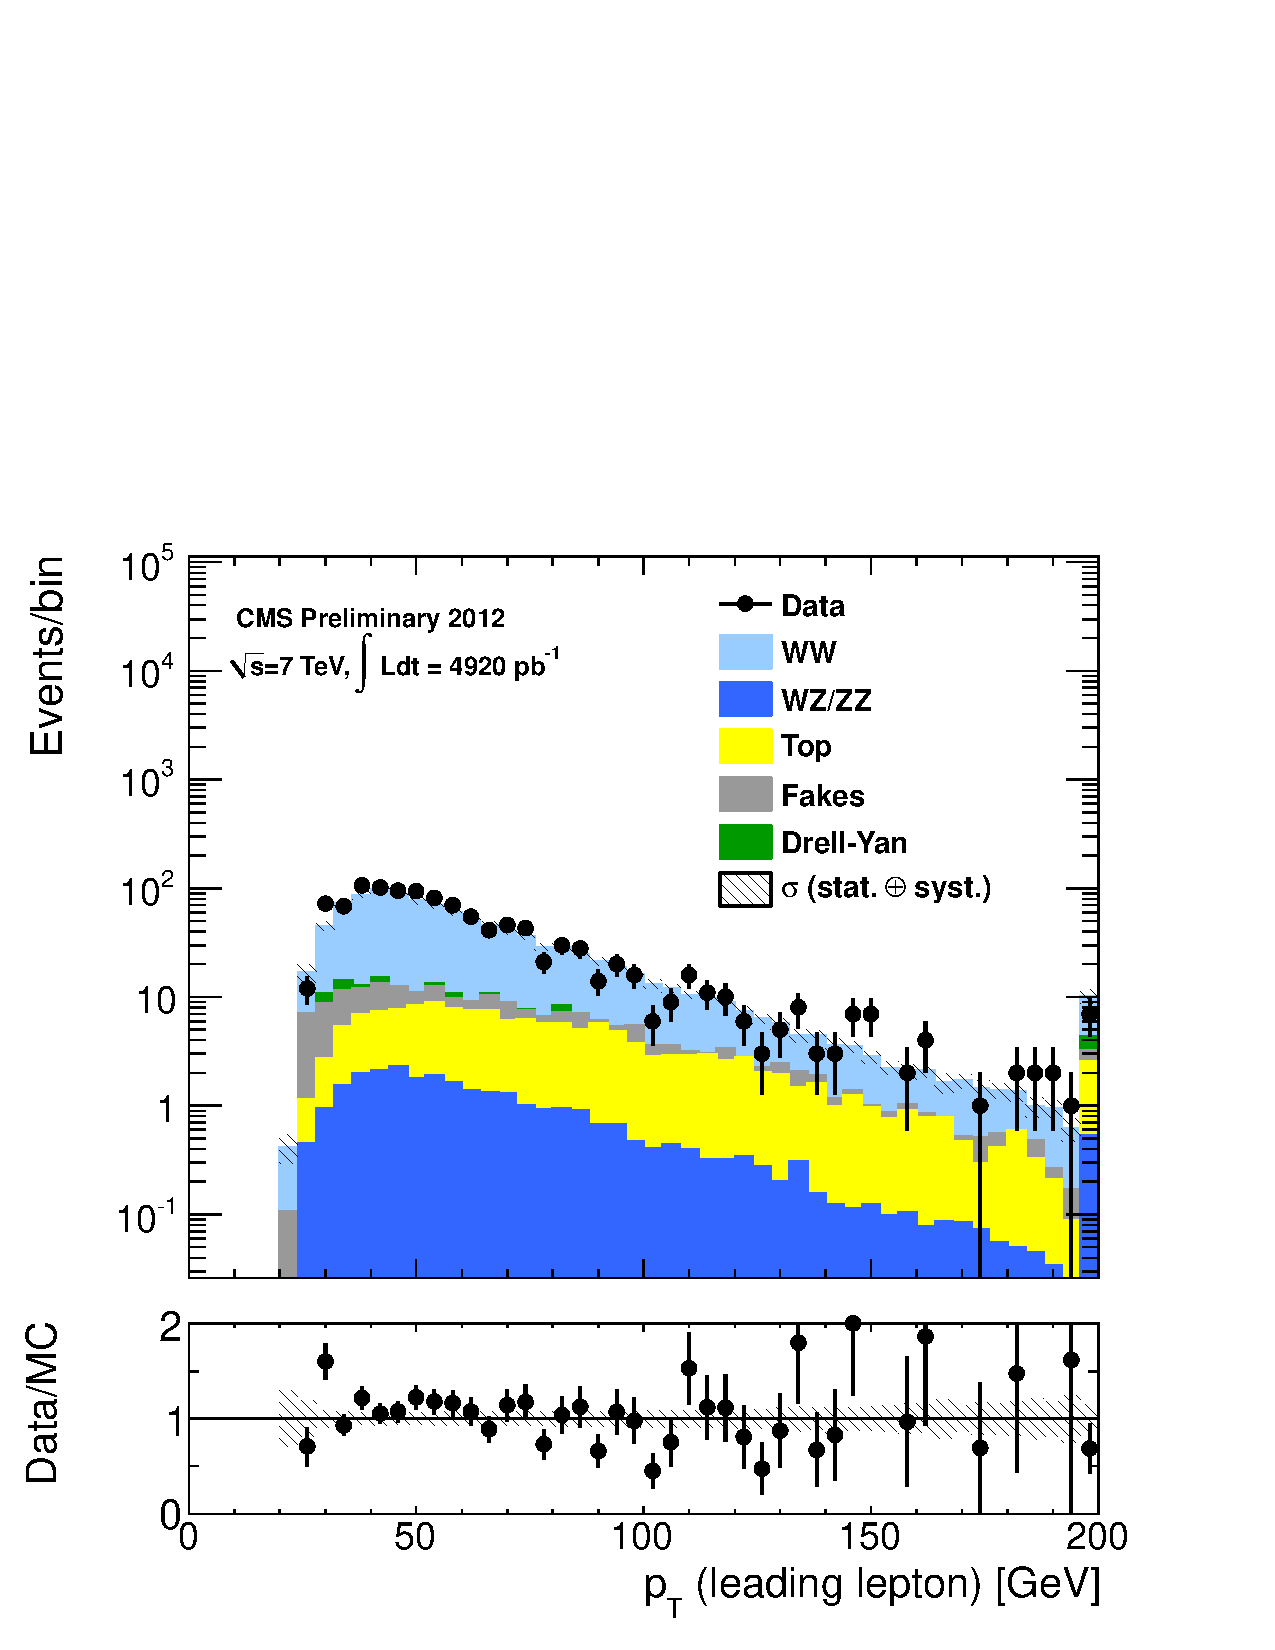
\includegraphics[width=.45\textwidth]{figures/pas_pt1_incl_log.pdf}}
\caption{Leading lepton \pt.}
\label{fig:pas_pt1_incl}
\end{figure}


  
\section{Data Samples}
  \label{sec:datasets}
  %UPDATEME%
The datasets used for this analysis are summarized in Tables.~\ref{tab:DatasetsData} 
and~\ref{tab:DatasetsMC} for data and Monte Carlo, respectively. The total integrated
luminosity is 49 $\pm$ 2 $\ipb$. We used just basic quality requirements, since an official good 
run list (JSON file) was not available. It will be used in future updates.
For Monte Carlo simulation we use madgraph when possible, 
but different generators such as Pythia and Powheg 
are also used. 
%For $gg \to \WW$ a dedicated generator is used. For \wz\ and \zz\
%processes we use Pythia, since MadGraph samples are mixed with $\WW$ in
%a single $VV$ sample, which is difficult to use properly.

%The choice of the Monte Carlo samples depends on the sample
%availability, but in general we tried to be consistent and use a
%single generator - MadGraph. In the case of Drell-Yan, MadGraph samples
%are not adequate to cover the full mass spectrum. The main sample has a 50 $\GeVcc$ 
%minimum dilepton mass requirement, while the other one, covering
%the low mass region, has an additional requirement on extra jet
%activity. 
%We use madgraph when possible, but different generators are used for some samples
%For $gg \to \WW$ a dedicated generator is used. For \wz\ and \zz\
%processes we use Pythia, since MadGraph samples are mixed with $\WW$ in
%a single $VV$ sample, which is difficult to use properly.

%UPDATEME%
\begin{table}[!ht]
\begin{center}
\begin{tabular}{|c|c|}
\hline
 Dataset Description                   &   Dataset Name   \\
\hline
\hline
\multicolumn{2}{|c|}{$H \to \WW$ Signal Selection Samples} \\
\hline
Run2011A MuEl PromptReco            &  /MuEG/Run2011A-PromptReco-v*/AOD   \\
Run2011A DiMuon PromptReco          &  /DoubleMu/Run2011A-PromptReco-v*/AOD   \\
Run2011A SingleMuon PromptReco      &  /SingleMu/Run2011A-PromptReco-v*/AOD   \\
Run2011A DiElectron PromptReco      &  /DoubleElectron/Run2011A-PromptReco-v*/AOD   \\
\hline
\hline
\multicolumn{2}{|c|}{Fake Rate Measurement Samples} \\
\hline
Run2010A Jet  PromptReco            & /Jet/Run2011A-PromptReco-v*/AOD	\\
Run2010B Photon PromptReco          & /Photon/Run2011A-PromptReco-v*/AOD \\
\hline
\end{tabular}
\caption{Summary of data datasets used.\label{tab:DatasetsData}}
\end{center}
\end{table}

\begin{table}[!ht]
\begin{center}
{\footnotesize
\begin{tabular}{|c|c|c|}
\hline
\multicolumn{3}{|c|}{With Pileup: Processed dataset name is always} \\
\multicolumn{3}{|c|}{/Spring11-PU\_S1\_START311\_V1G1-v*/AODSIM} \\
\hline
 Dataset Description                     &   Primary Dataset Name   & cross-section (pb)\\
\hline
qq $\rightarrow WW$                  	 &   /VVJetsTo4L\_TuneD6T\_7TeV-madgraph-tauola                        &  43.0  \\
gg $\rightarrow WW \to 2l 2\nu$          &   /GluGluToWWTo4L\_TuneZ2\_7TeV-gg2ww-pythia6                       &   0.153\\
$\ttbar$                              	 &   /TTJets\_TuneZ2\_7TeV-madgraph-tauola                             & 157.5 \\
$\singletops$                  	 	 &   /TToBLNu\_TuneZ2\_s-channel\_7TeV-madgraph                        &  1.4 \\
$\singletopt$                  	 	 &   /TToBLNu\_TuneZ2\_t-channel\_7TeV-madgraph                        &  20.9 \\
tW                                    	 &   /TToBLNu\_TuneZ2\_tW-channel\_7TeV-madgraph                       &  10.6 \\
Z[20-inf] $\rightarrow ee$	  	 &   /DYToEE\_M-20\_CT10\_TuneZ2\_7TeV-powheg-pythia                   &  1666.0 \\
Z[20-inf] $\rightarrow \mu\mu$        	 &   /DYToMuMu\_M-20\_CT10\_TuneZ2\_7TeV-powheg-pythia                 &  1666.0 \\	       
Z[20-inf] $\rightarrow \tau\tau$  	 &   /DYToTauTau\_M-20\_CT10\_TuneZ2\_7TeV-powheg-pythia-tauola        &  1666.0 \\
Z[10-20]  $\rightarrow ee$	  	 &   /DYToEE\_M-10To20\_CT10\_TuneZ2\_7TeV-powheg-pythia               &  3892.9 \\
Z[10-20]  $\rightarrow \mu\mu$    	 &   /DYToMuMu\_M-10To20\_CT10\_TuneZ2\_7TeV-powheg-pythia             &  3892.9 \\
Z[10-20]  $\rightarrow \tau\tau$  	 &   /DYToTauTau\_M-10To20\_CT10\_TuneZ2\_7TeV-powheg-pythia-tauola    &  3892.9 \\
W/Z+$\gamma$                       	 &   /PhotonVJets\_7TeV-madgraph                                       &  165.0 \\
W $\rightarrow$ $\ell\nu$           	 &   /WJetsToLNu\_TuneZ2\_7TeV-madgraph-tauola                         &  31314.0 \\
WZ                               	 &   /WZtoAnything\_TuneZ2\_7TeV-pythia6-tauola                        &  18.2 \\
ZZ                               	 &   /ZZtoAnything\_TuneZ2\_7TeV-pythia6-tauola                        &   5.9\\
$gg \to H \to WW \to 2\ell2\nu$          &   /GluGluToHToWWTo2L2Nu\_M-*\_7TeV-powheg-pythia6                   & vary \\
$gg \to H \to WW \to \ell\tau2\nu$       &   /GluGluToHToWWTo2L2Nu\_M-*\_7TeV-powheg-pythia6                   & vary \\
$gg \to H \to WW \to 2\tau2\nu$          &   /GluGluToHToWWTo2Tau2Nu\_M-*\_7TeV-powheg-pythia6                 & vary \\
$qqH,~H \to WW \to 2\ell2\nu$            &   /VBF\_HToWWTo2L2Nu\_M-*\_7TeV-powheg-pythia6                      & vary \\
$qqH,~ H \to WW \to \ell\tau2\nu$	 &   /VBF\_HToWWTo2Tau2Nu\_M-*\_7TeV-powheg-pythia6                    & vary \\
$qqH,~H \to WW \to 2\tau2\nu$	         &   /VBF\_HToWWToLNuTauNu\_M-*\_7TeV-powheg-pythia6                   & vary \\
$WH/ZH/\ttbar H,~H\to WW$                &   /WH\_ZH\_TTH\_HToWW\_M-*\_7TeV-pythia6                            & vary \\
\hline
\hline
\end{tabular}
}
\caption{Summary of Monte Carlo datasets used.\label{tab:DatasetsMC}. The cross sections for a SM Higgs boson
is taken from the LHC Higgs cross-section working group~\cite{LHCHiggsCrossSectionWorkingGroup:2011ti}}
\end{center}
\end{table}

Due to details in the implementation of the Powheg calculation, the
resulting Higgs $\pt$ spectrum for $gg \to H$ has a much harder
spectrum compared with the most precise spectrum calculated to NNLO
with resummation to NNLL order, as illustrated in
Figure~\ref{fig:h160ww_pthiggs}(a). Therefore, the proper procedure is
to apply an event-by-event rewighting to the Powheg simulated
events. For the time being we correct the $gg \to H \to \WW$ jet bin
efficiency computed from the Powheg Monte Carlo sample, by a scale
factor which is approximately identical for all Higgs masses. The
scale factors applied to each jet bin in the Powheg simulation are
shown in Figure~\ref{fig:h160ww_pthiggs}(b). The jet definition is 
consitent with the one used in the analysis.

\begin{figure}[!htbp]
\begin{center}
   \subfigure[]{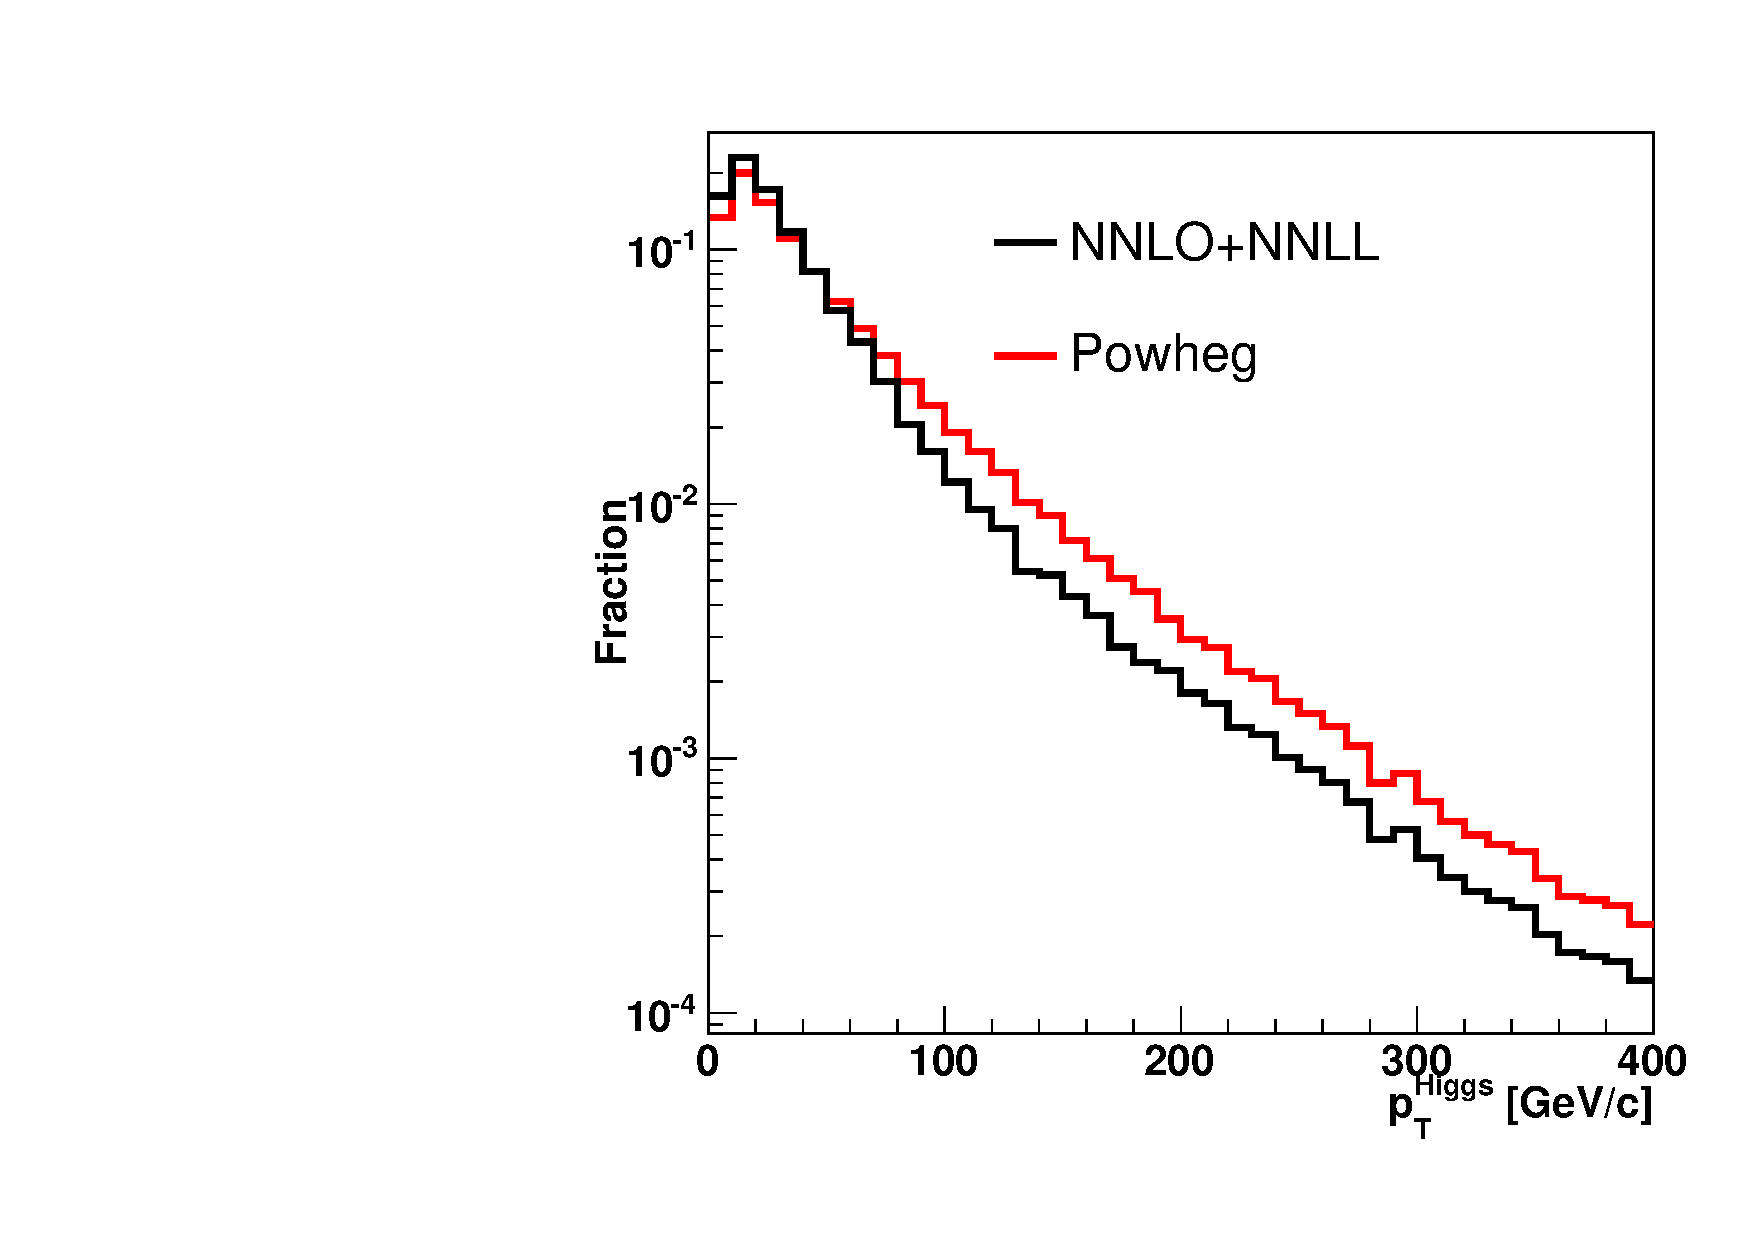
\includegraphics[width=0.49\textwidth]{figures/h160ww_pthiggs.pdf}}
   \subfigure[]{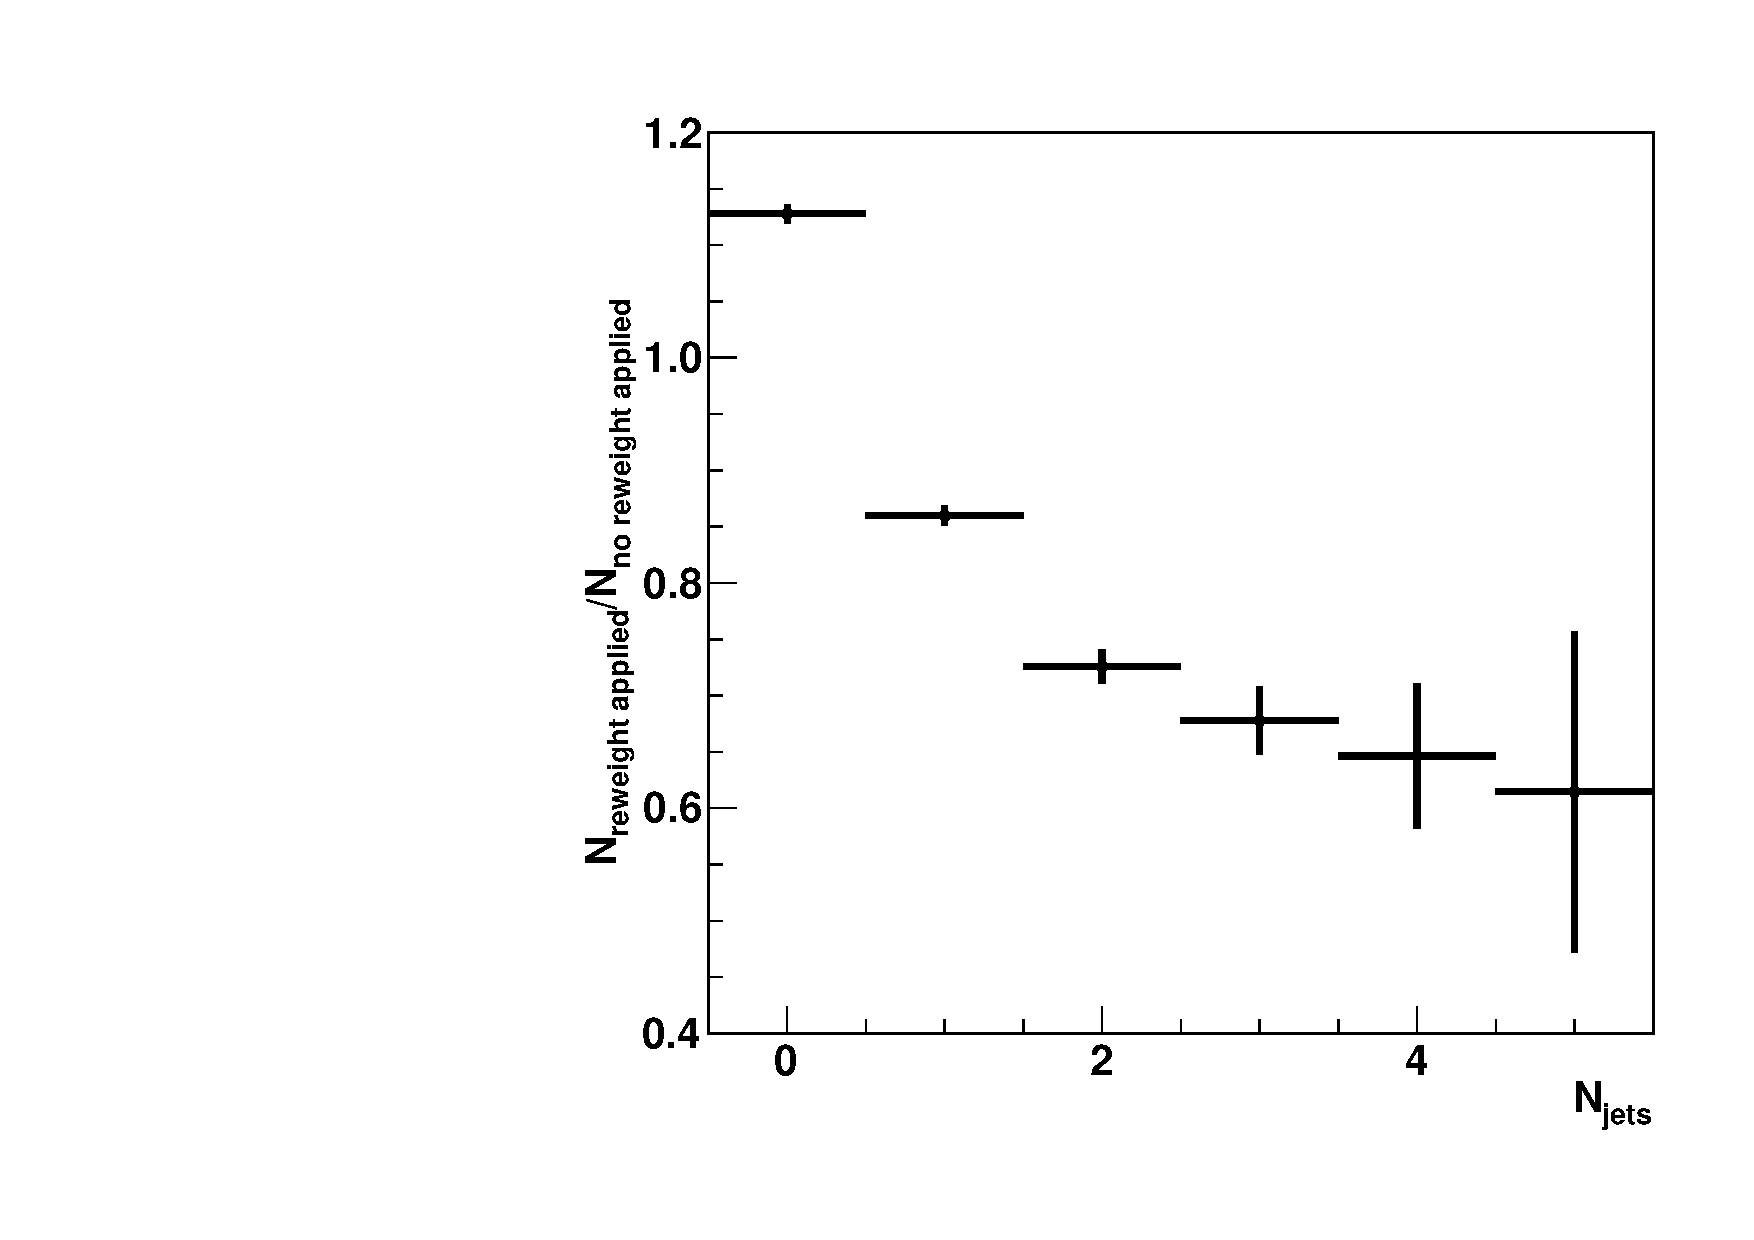
\includegraphics[width=0.49\textwidth]{figures/h160ww_njets_kfactor_ratio.pdf}} 
\caption{(a) Higgs transverse momentum spectrum as predicted by Powheg and the NNLO+NNLL calculation; (b) 
scale factors applied to each jet bin in the Powheg simulation.}
\label{fig:h160ww_pthiggs}
\end{center}
\end{figure}

  
\section{Event Selection}
  \label{sec:selection} 
  The fully leptonic final state consists of two isolated leptons
and large missing energy from the two undetectable neutrinos.
The major reducible background processes are \ttbar{}, \wjets{} and Drell-Yan. 
We thus perform several steps to select and extract the $\WW$ signal from data:

\begin{enumerate}
    \item We select events that pass pre-defined lepton triggers.
    \item We then select those events with two oppositely charged 
    high $\pt$ isolated leptons ($ee$, $\mu\mu$, $e\mu$) requiring:
        \begin{itemize}    
            \item $\pt>20~\GeVc$ for both leptons;
            \item standard identification and isolation requirements 
	    on both leptons.
        \end{itemize}
     \item We reject events with more than zero reconstructed jets;
     \item large transverse missing energy due to the neutrinos.
\end{enumerate}

The selection steps are now described in detail in Ref. \cite{ref:WWXS2011}.


   \subsection{Trigger}
     \label{sec:sel_trigger}
     Triggering on Higgs boson decays in the dilepton final state increases 
in difficulty with increasing instantaenous luminosity.
Single lepton triggers can only be sustained with very tight identification and
isolation requirements and large transverse momentum thresholds.
This means that double lepton triggers are the only viable option to maintain
sensitivity to a low mass Higgs boson, where the leptons transverse momentum
can be small.

We use a suite of signal and control triggers designed in the $H \to \WW$ analysis~\cite{HWW2011AN}. 
These dilepton triggers have a high efficiency to collect Higgs boson events
and are sufficiently loose to collect control events to estimate the 
selection efficiencies and with adequate precision.
%We describe the features and motivations for the analysis triggers in Section~\ref{sec:mainTriggers},
%and additional triggers to collect control events in 
%Section~\ref{sec:utilityTriggers}.

%\subsubsection{Analysis Triggers}
%\label{sec:mainTriggers}

The main dielectron triggers, described in Table~\ref{tab:triggers_ee}, require two HLT electron
candidates with loose shower shape and calorimeter isolation requirements on both legs
and a match to a Level-1 seed for the leading leg.
To accomodate the offline selection of $E_{T}>30,20$~GeV for the leading and trailing
electrons, $E_{T}>17,8$~GeV is required at the HLT level.
The main dimuon triggers
require two HLT muon candidates with transverse momentum greater than $7$~$\GeVc$ and
a match to a Level-1 seed is required for both legs.
These are described in Table~\ref{tab:triggers_mm}.

%%%%%%%%%
\begin{table}[!ht]
  \caption{Analysis triggers for the $ee$ final state. 
The identification and isolation requirements are described in Ref.~\cite{HWW2011AN}}.
    \vspace{5pt}
   \label{tab:triggers_ee}
  \begin{center}
 {\small
  \begin{tabular} {l|l|l|c}
\hline
  Dataset & Trigger name & L1 seed & Description\\
  \hline \hline
  \multirow{2}{*}{DoubleElectron} & HLT\_Ele17\_CaloIdL\_CaloIsoVL\_&  L1\_SingleEG12  & $p_T>17,8~\GeVc$ \\
                                  & Ele8\_CaloIdL\_CaloIsoVL &                  & \\

  \multirow{2}{*}{DoubleElectron} & HLT\_Ele17\_CaloIdT\_TrkIdVL\_CaloIsoVL\_TrkIsoVL\_ &  L1\_SingleEG12  & $p_T>17,8~\GeVc$ \\
                                  & Ele8\_CaloIdT\_TrkIdVL\_CaloIsoVL\_TrkIsoVL &                  & \\
  \hline
  \end{tabular}
}
  \end{center}
\end{table}
%%%%%%%%%

%%%%%%%%%
\begin{table}[!ht]
  \caption{Analysis triggers for the $\mu\mu$ final state. Triggers marked (*) are also used for efficiency studies.}
    \vspace{5pt}
   \label{tab:triggers_mm}
  \begin{center}
 {\small
  \begin{tabular} {l|l|l|c}
\hline
  Dataset & Trigger name & L1 seed & Description\\
  \hline \hline
  DoubleMu & HLT\_DoubleMu6 & L1\_DoubleMu3  & $p_T>6,6~\GeVc$\\
  DoubleMu & HLT\_DoubleMu7 & L1\_DoubleMu3  & $p_T>7,7~\GeVc$ \\
  DoubleMu & HLT\_Mu13\_Mu8 & L1\_DoubleMu3  & $p_T>13,8~\GeVc$ \\
  DoubleMu & HLT\_Mu17\_Mu8 & L1\_DoubleMu3  & $p_T>17,8~\GeVc$ \\
  \hline
  \end{tabular}
}
  \end{center}
\end{table}
%%%%%%%%%

%%%%%
\begin{table}[!ht]
  \caption{Single lepton triggers to recover lost efficiency. These trigges are also used for efficiency studies.
The identification and isolation requirements for electrons are described in Table~\ref{tab:HLTElectronCuts}.}
    \vspace{5pt}
   \label{tab:triggers_single}
  \begin{center}
 {\small
  \begin{tabular} {l|l|l|c}
\hline
  Dataset & Trigger name & L1 seed & Description\\
  \hline \hline
  SingleEle & HLT\_Ele27\_CaloIdVT\_CaloIsoT\_TrkIdT\_TrkIsoT & L1\_SingleEG15  & $p_T>27~\GeVc$ \\
  \hline \hline
  SingleMu & HLT\_IsoMu12   & L1\_SingleMu7  & $p_T>12~\GeVc$ \\
  SingleMu & HLT\_IsoMu17   & L1\_SingleMu10 & $p_T>17~\GeVc$ \\
  SingleMu & HLT\_Mu15      & L1\_SingleMu10 & $p_T>15~\GeVc$ \\
  \hline 
  \end{tabular}
}
  \end{center}
\end{table}
%%%%%


%\subsubsection{Utility Triggers}
%\label{sec:utilityTriggers}

%We now describe additional triggers that are introduced to collect control or
%calibration events not covered by the main analysis triggers.

To estimate the non-$Z$ dilepton backgrounds, where the selected dileptons are 
not from the $Z$ details, we need to use the events collected in the $e\mu$ final sates. 
In the electron-muon channel we use two complementary triggers, which require
both muon and electron HLT candidates.
These are summarised in Table~\ref{tab:triggers_em}.
Finally, to recover any residual inefficiency,
we also allow events that passed only the single electron
or single isolated muon triggers summarised in Table~\ref{tab:triggers_single}.

%%%%%
\begin{table}[!ht]
  \caption{Analysis triggers for the $e\mu$ final state.
The identification and isolation requirements for electrons are described in Ref.~\cite{HWW2011AN}.}
    \vspace{5pt}
   \label{tab:triggers_em}
  \begin{center}
 {\small
  \begin{tabular} {l|l|l|c}
\hline
  Dataset & Trigger name & L1 seed & Description\\
  \hline \hline
  MuEG & HLT\_Mu17\_Ele8\_CaloIdL & L1\_Mu3\_EG5 & $p_T>17,8~\GeVc$ \\
  MuEG & HLT\_Mu8\_Ele17\_CaloIdL & L1\_Mu3\_EG5 & $p_T>8,17~\GeVc$ \\
 \hline
  \end{tabular}
}
  \end{center}
\end{table}
%%%%%

Because the main dielectron analysis triggers make requirements on
both legs, events collected with those triggers cannot be used to measure
efficiencies without introducing unacceptable bias.
Thus, to measure the electron selection and trigger efficiency
we introduce two specialised tag and probe triggers designed to maximize
the number of useful \dyll~events, % for both low and high $p_{T}$ electrons,
while keeping the total trigger rate at a reasonable level. 
%The tag and probe method is described later in Section~\ref{sec:efficiency}.

%The first trigger probes low $p_T$ electrons and applies very tight identification 
%and isolation requirements on the tag leg to reduce the background rate.
%The second trigger probes higher $p_{T}$ electrons.
%Both triggers are described in Table~\ref{tab:triggers_util} and labeled "eff".

Another set of specialised triggers are used to record events
enriched in fake electrons and muons for the measurement of jet induced backgrounds.
This is done using the fake rate method, which is described in detail in ref.~\ref{sec:HWW2011AN}. 
{\bf \fixme{} Add the photon jet triggers..}

   \subsection{Primary Vertex Reconstruction}
     \label{sec:sel_pv}
     Primary vertices are reconstructed using the so-called Deterministic Annealing (DA) 
clustering of tracks~\cite{PVDA}. Reconstructed primary vertices are required to have a
$z$ position within 24~cm of the nominal detector center and a radial position within 
2~cm of the beamspot. There must also be greater than four degrees of freedom in
the fitted vertex. From the set of primary vertices in the event passing these
selection cuts, the vertex with the largest summed squared-$\pt$ of the associated
tracks is chosen as the event primary vertex. Reconstructed leptons will be required 
to have small impact parameters with respect to this vertex.

Due to the fast evolution of the LHC machine, with a rapid rise in the
instantaneous luminosity, the data taking conditions have changed
rapidly.  In particular it is difficult to exactly reproduce the
number of overlapping events (i.e. pileup) between data and
simulation, and thus there will be differences in the number of
reconstructed primary vertices. 
To make sure the simulation reproduces the data, we reweight the number of
primary verteces in the simulation to match the distribution observed in the 
data, after requiring that the event has two leptons passing offline
lepton selection.

   \subsection{Muon Selection} 
     \label{sec:sel_muons}
    Muons in CMS are reconstructed as either $StandAloneMuons$ (track
in the muon detector with low momentum resolution), $GlobalMuons$
(outside-in approach seeded by a $StandAloneMuon$ with a global fit
using hits in the muon, silicon strip and pixel 
detectors) and $TrackerMuons$ (inside-out approach seeded by an offline 
silicon strip track, using the muon detector only for muon identification 
without refitting the track). Most good quality muons are reconstructed as 
all three types at the same time and the momentum resolution is dominated by the inner
tracker system up to about 200~$\GeVc$ in transverse momentum. Details about the
optimization at low $\pt$ are given in Appendix~\ref{app:mus}. The specific
requirements to select good prompt isolated muons are the following:
\begin{itemize}
\item the muon must be found by both the global and tracker muon algorithms;
\item the global muon must have at least one good muon hit;
\item the tracker muon must have at least two matches to muon segments in 
      different muon stations;
\item more than 10 hits in the inner tracker;
\item at least one pixel hit;
\item $\chi^2/{\mathrm{ndof}} < 10$ on a global fit;
\item impact parameter in the transverse plane $|d_{0}| < 0.02~(0.01)$~cm for
      muons with $\pt$ greater (smaller) than 20 $\GeVc$,
      calculated with respect to the primary vertex;
\item longitudinal impact parameter $|d_{z}| <0.2$~cm,
      calculated with respect to the primary vertex;
\item pseudorapidity $|\eta|$ must be smaller than 2.4;
\item relative \pt\ resolution is better than 10\%.
\end{itemize}

Furthermore, the particle flow candidate-based isolation variable is 
used to reduce the contamination from the non-isolated muons originating from
jets. 

\begin{itemize}
\item $\rm{Iso}_{PF}$: defined as the scalar sum of the \pt\ of the 
    particle flow candidates satisfying the following requirements:
    \begin{itemize}
    \item $\Delta R~<~0.3$ to the muon in the $\eta \times \phi$ plane,
    \item $|d_{z}(\mathrm{PF Candidate}) - d_{z}(\mathrm{muon})| < 0.1$~cm, if the PF candidate is charged,
    \item \pt $>1.0$ GeV, if the PF candidate is classified as a neutral hadron or a photon.
    \end{itemize}
\end{itemize}

We require $\frac{\rm{Iso}_{PF}}{\pt}~<~0.13~(0.06)$ for muons in the barrel 
with $\pt$ greater (smaller) than 20 $\GeVc$. For muons in the endcap, we
require $\frac{\rm{Iso}_{PF}}{\pt}~<~0.09~(0.05)$ for muons with $\pt$ 
greater (smaller) than 20 $\GeVc$. Further details of the choice of
the isolation requirement is documented in Appendix \ref{app:pfIsoStudy}.


   \subsection{Electron Selection} 
     \label{sec:sel_electrons}
     We identify electrons using a multivariate approach optimized 
for this analysis~\cite{MVAElId}. In addition, we require some minimal 
requirements to make sure the electron candidate is as tight as the 
trigger selection:

\begin{itemize}
  \item $p_T>10$~GeV and $|\eta| < 2.5$
  \item $\sigma_{i\eta i\eta} < 0.01/0.03$ (barrel/endcap)
  \item $|\Delta\phi_{in}| < 0.15/0.10$
  \item $|\Delta\eta_{in}| < 0.007/0.009$
  \item $H/E< 0.12/0.10$ (barrel/endcap)
  \item $\frac{\sum_{\rm trk}\Et}{\pt^{\rm ele}}<0.2$
  \item $\frac{\sum_{\rm ECAL}\Et}{\pt^{\rm ele}}<0.2$
  \item $\frac{\sum_{\rm HCAL}\Et}{\pt^{\rm ele}}<0.2$
\end{itemize}

Isolation requirements are then imposed by computing the particle flow isolation,
defined as the scalar sum of the \pt\ of the particle flow candidates satisfying 
the following requirements:

\begin{itemize}
\item $\Delta R~<~0.4$ to the electron in the $\eta \times \phi$ plane,
\item for neutral hadron PF candidates, require that it is outside the footprint veto region of $\Delta R~<~0.07$,
\item for photon and electron PF candidates, require that it is outside the footprint veto region of $|\Delta\eta|<0.025$,
\item $|d_{z}(\mathrm{PF~candidate}) - d_{z}(\mathrm{muon})| < 0.1$~cm, if the PF candidate is charged,
\item \pt $>1.0$ GeV, if the PF candidate is classified as a neutral hadron or a photon.
\end{itemize}

We require $\frac{\rm{Iso}_{PF}}{\pt}~<~0.13~(0.09)$ for electrons in the barrel (endcap).

In order to veto fake electrons from converted photons, 
we look for a reconstructed conversion vertex where one of the two tracks 
is compatible with the electron~\cite{ConversionNote}.
The vertex fit probability is required to be $>10^{-6}$.
We then require that there are no missing expected missing hits forming the electron track~\cite{ConversionNote},~\cite{NExpHits}. 
Finally to reduce fake electrons from non-prompt sources,
we require the transverse and longitudinal impact parameters with
respect to the primary vertex to be less than $0.02$ and $0.1$~cm respectively.

   \subsection{Missing Energy} 
     \label{sec:sel_met}
     
The missing transverse energy is used to reject background events
where there is no natural source of missing energy, like in Drell-Yan and
QCD events. In the $\dytt$ process there is a large difference in the masses of 
$\tau$ and $\Z$. The taus are produced with large boost and their decay products, including 
neutrinos, are aligned with the leptons. Therefore a transverse component 
of missing energy with respect to the leptons is a better measure of true 
missing energy in the event, not originating from $\tau$ decay. 
To reject such background events with a small opening angle
between \met\ and one of the leptons, we used the projected \met~\cite{HWW2010} for 
event selection, defined as:
\begin{equation}
\text{with } \Delta\phi_{min} =  min(\Delta\phi(\ell_1,\met),\Delta\phi(\ell_2,\met))\\
\end{equation}
\begin{equation}
= 
\begin{cases} \met & \text{if $\Delta\phi_{min}>\frac{\pi}{2}$,}
\\
\met\sin(\Delta\phi_{min}) & \text{if $\Delta\phi_{min}<\frac{\pi}{2}$}
\end{cases}
\end{equation}
where $\Delta\phi(\ell_i,\met)$ is the angle between \met\ and lepton
 $i$ in the transverse plane.

In the presence of high multiple-interactions (pile-up), the instrumental \met\ tail in 
$\dyll$ events increases significantly. 
Figure~\ref{fig:met_pu} shows the projected particle-flow MET~\cite{PFMET} in the 
events with low ($<$5) and high ($>5$) primary vertices in both $\dyll$ data and MC. 
The $\dyll$ events in data are selected by requiring the dilepton invariant mass 
within 15 $\GeVcc$ of the $Z$ mass. 
This leads to a large increase of the background contribution in the signal region, as shown in 
Figure~\ref{fig:meteff_pu}. 
%This causes a sharp increase in the efficiency for $\dyll$ events to pass a given \met\ 
%requirement as the number of pile-up interactions increases. 
%To improve the robustness of the \met\ performance in the presence of pile-up, 
To improve the signal over background performance of \met\ selections in the presence of pile-up, 
we have developed a novel \met\ algorithm referred to as ``trk-MET''~\cite{FIXME}, constructed from 
charged particles consistent with originating from the primary vertex. 
The event $\met$ trk-MET is defined as 
\begin{equation}
\text{trk-MET} \equiv -\overrightarrow{p_T}(l_1) - \overrightarrow{p_T}(l_2) - \sum_i{\overrightarrow{p_T}(i)}, \\
\label{eq:trkmet}
\end{equation}
where $\overrightarrow{p_T}(l_1)$ and $\overrightarrow{p_T}(l_2)$ are the transverse momentum vectors of the two 
leptons passing the lepton selections described in Section~\ref{sec:sel_muons}-\ref{sec:sel_electrons}, 
and $\overrightarrow{p_T}(i)$ represent the tranverse momentum vectors of the charged PFCandidates satisfying the following requirements:
%%%%%%%%%%%%%%%%%%%%%%%%%%
\begin{itemize}
\item the track matched to PFCandidate has $\Delta z < 0.1$~cm with respect to the signal PV, which is the 
closest PV to the track in $\Delta z$;
\item the track has $\Delta R > 0.1$ with respect to both leptons, to avoid double-counting of the leptons.
\end{itemize}
%%%%%%%%%%%%%%%%%%%%%%%%%%

Comparing to the projected PFMet, we observed that the projected trk-MET has 
a larger tail in $\dyll$ background events~\cite{FIXME}. 
However these two \met\ values are weakly-correlated in $\dyll$ backgrounds with no geninue $\met$, and 
strongly correlated for the signal processes with geninue $\met$, as shown in Figure~\ref{fig:met_scatter}. 
Therefore the signal over background ratio is optimized if we select the events 
based on the mininum of these two projected $\met$ values, $\text{min-MET} \equiv min(\text{proj}_\text{trk-MET}, \text{proj}_\text{PFMET})$. 


The selection requirements are different between \ee{}/\mm{}
and \emu{} final states since Drell-Yan mostly contributes to \ee\
and \mm\ channels. The selection requirements are:
\begin{itemize}
\item projected $\met>20~\GeV$ for \emu{}
\item projected $\met>35~\GeV$ for \ee{} and \mm{} 
\end{itemize}
The selection efficiencies for the signal ($\hww$ at $m_{H}=130$ GeV) and background ($\dyll$) 
events are shown in Figure~\ref{fig:met_eff} as a function of $\met$ requirements. 
Using min-MET we see that the signal selection efficiency improves while the background selection efficiency reduces significantly 
compared to the values obtained using projected PFMet. 
In addition, the background selection efficiency dependendence on the 
number of primary vertices is largely reduced as well using min-MET. 


%%%%%%%%%%%%%%%%%%%%%%%%%%%%%%%%%%%%%%%%%%%
\begin{figure}[hbt]
\begin{center}
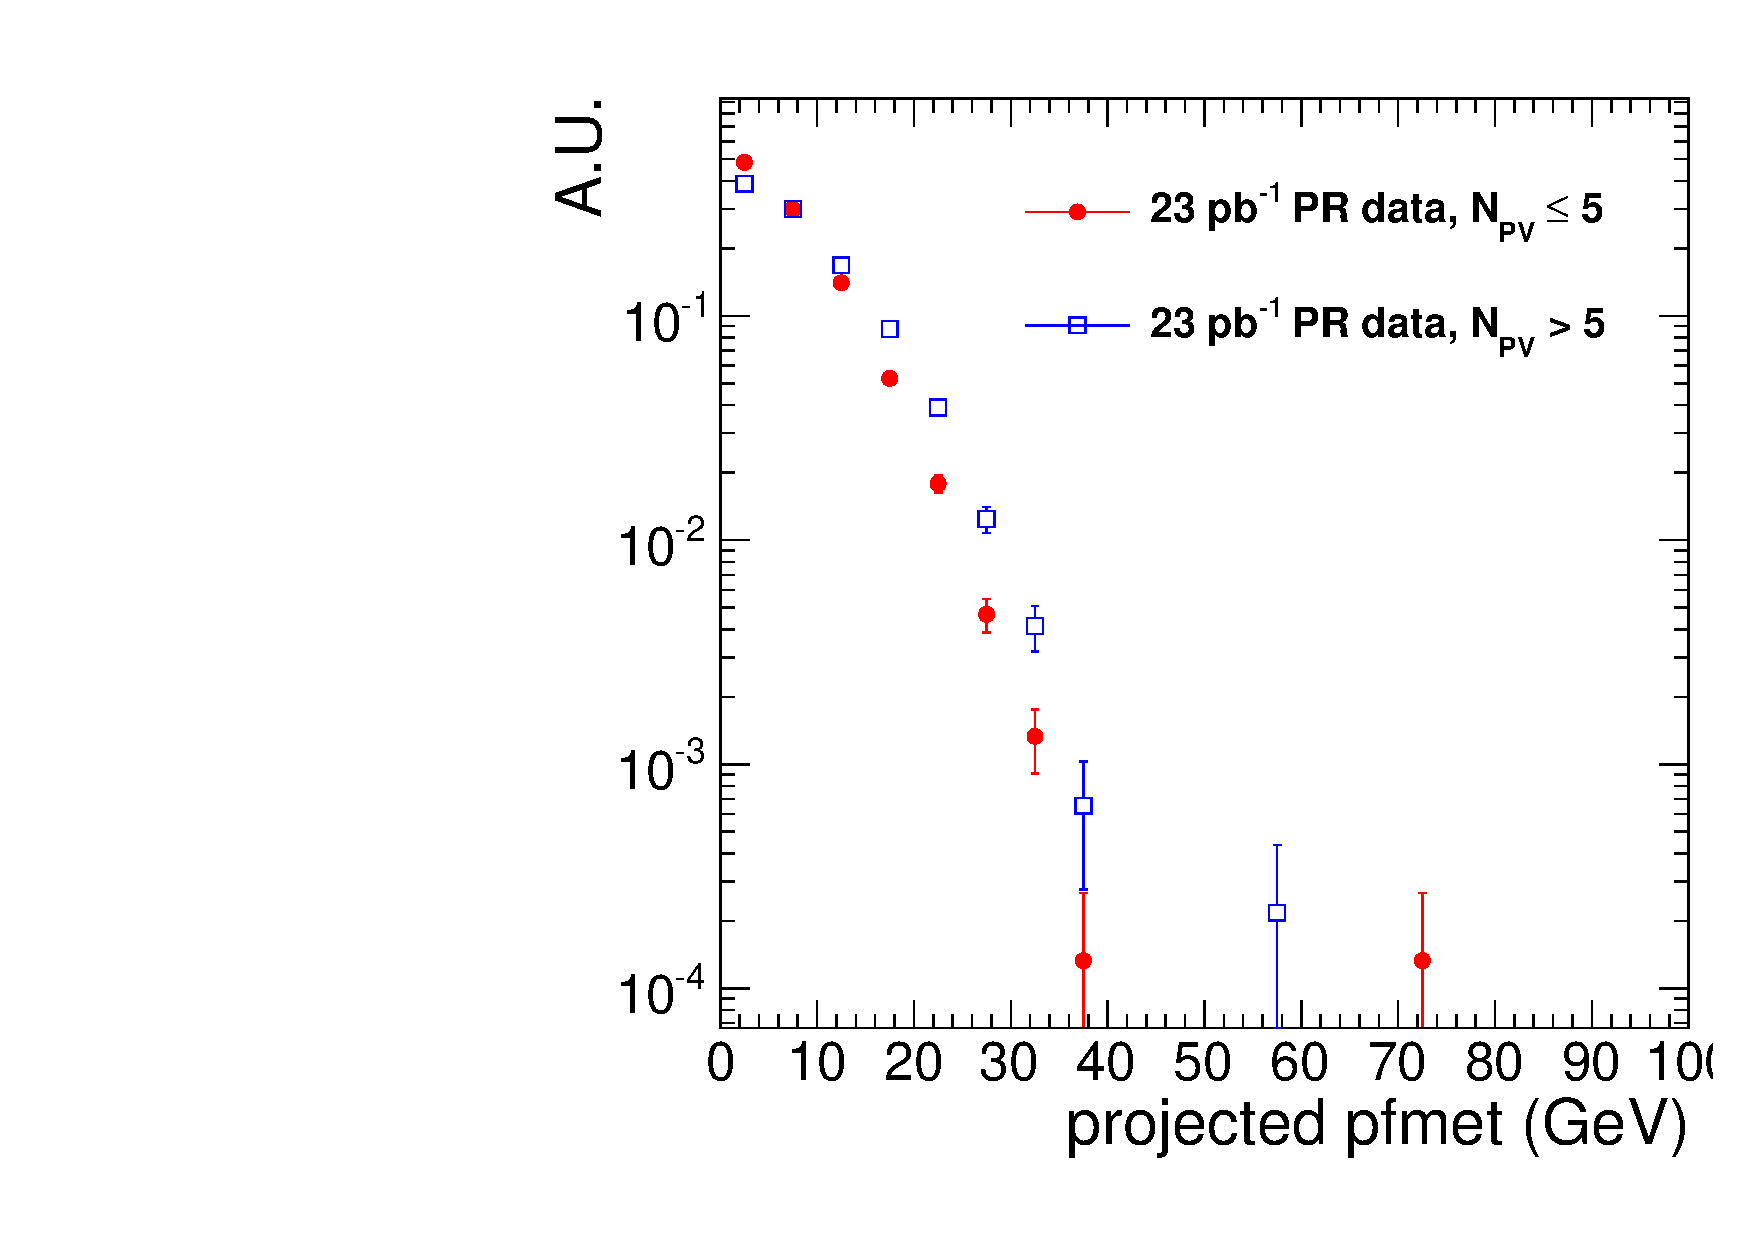
\includegraphics[width=0.4\linewidth]{figures/pfmet_data.pdf} 
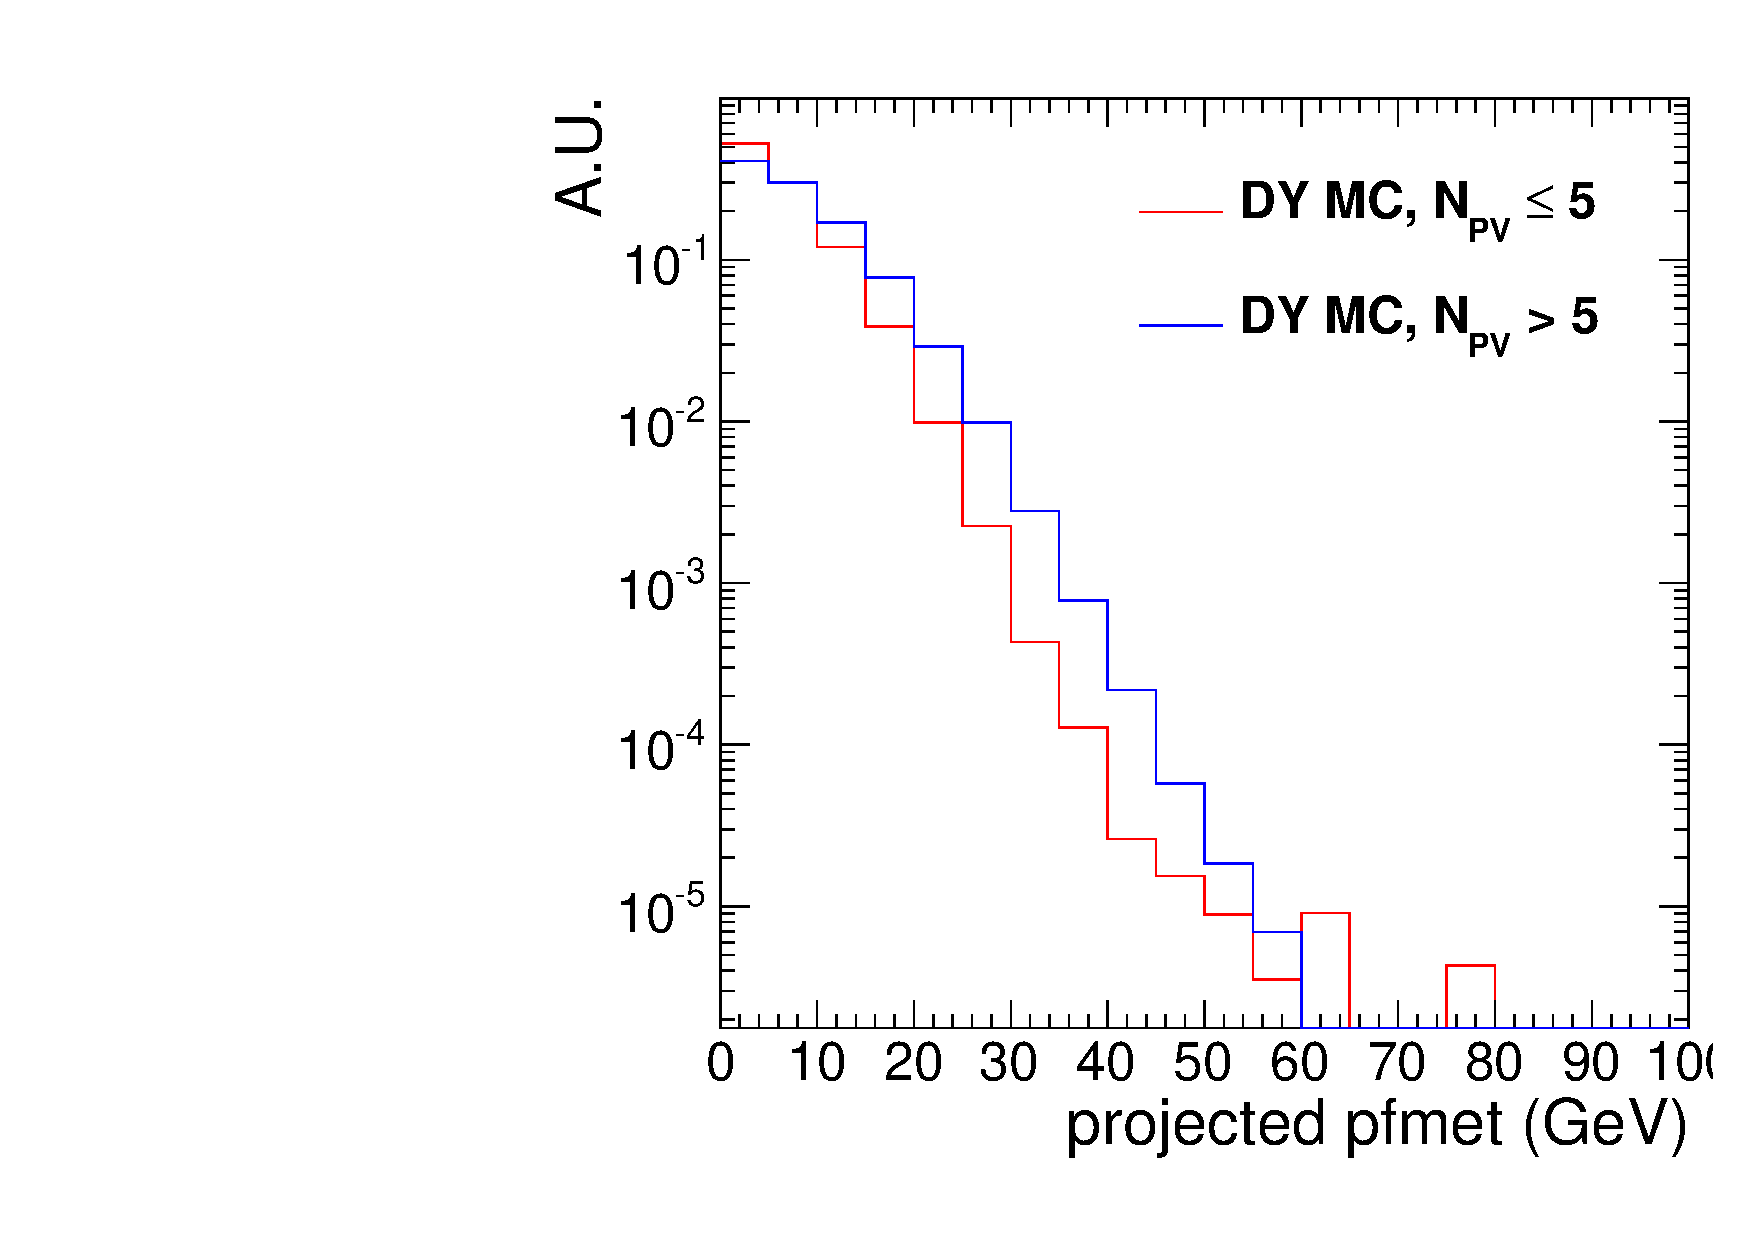
\includegraphics[width=0.4\linewidth]{figures/pfmet_dymc.pdf}
%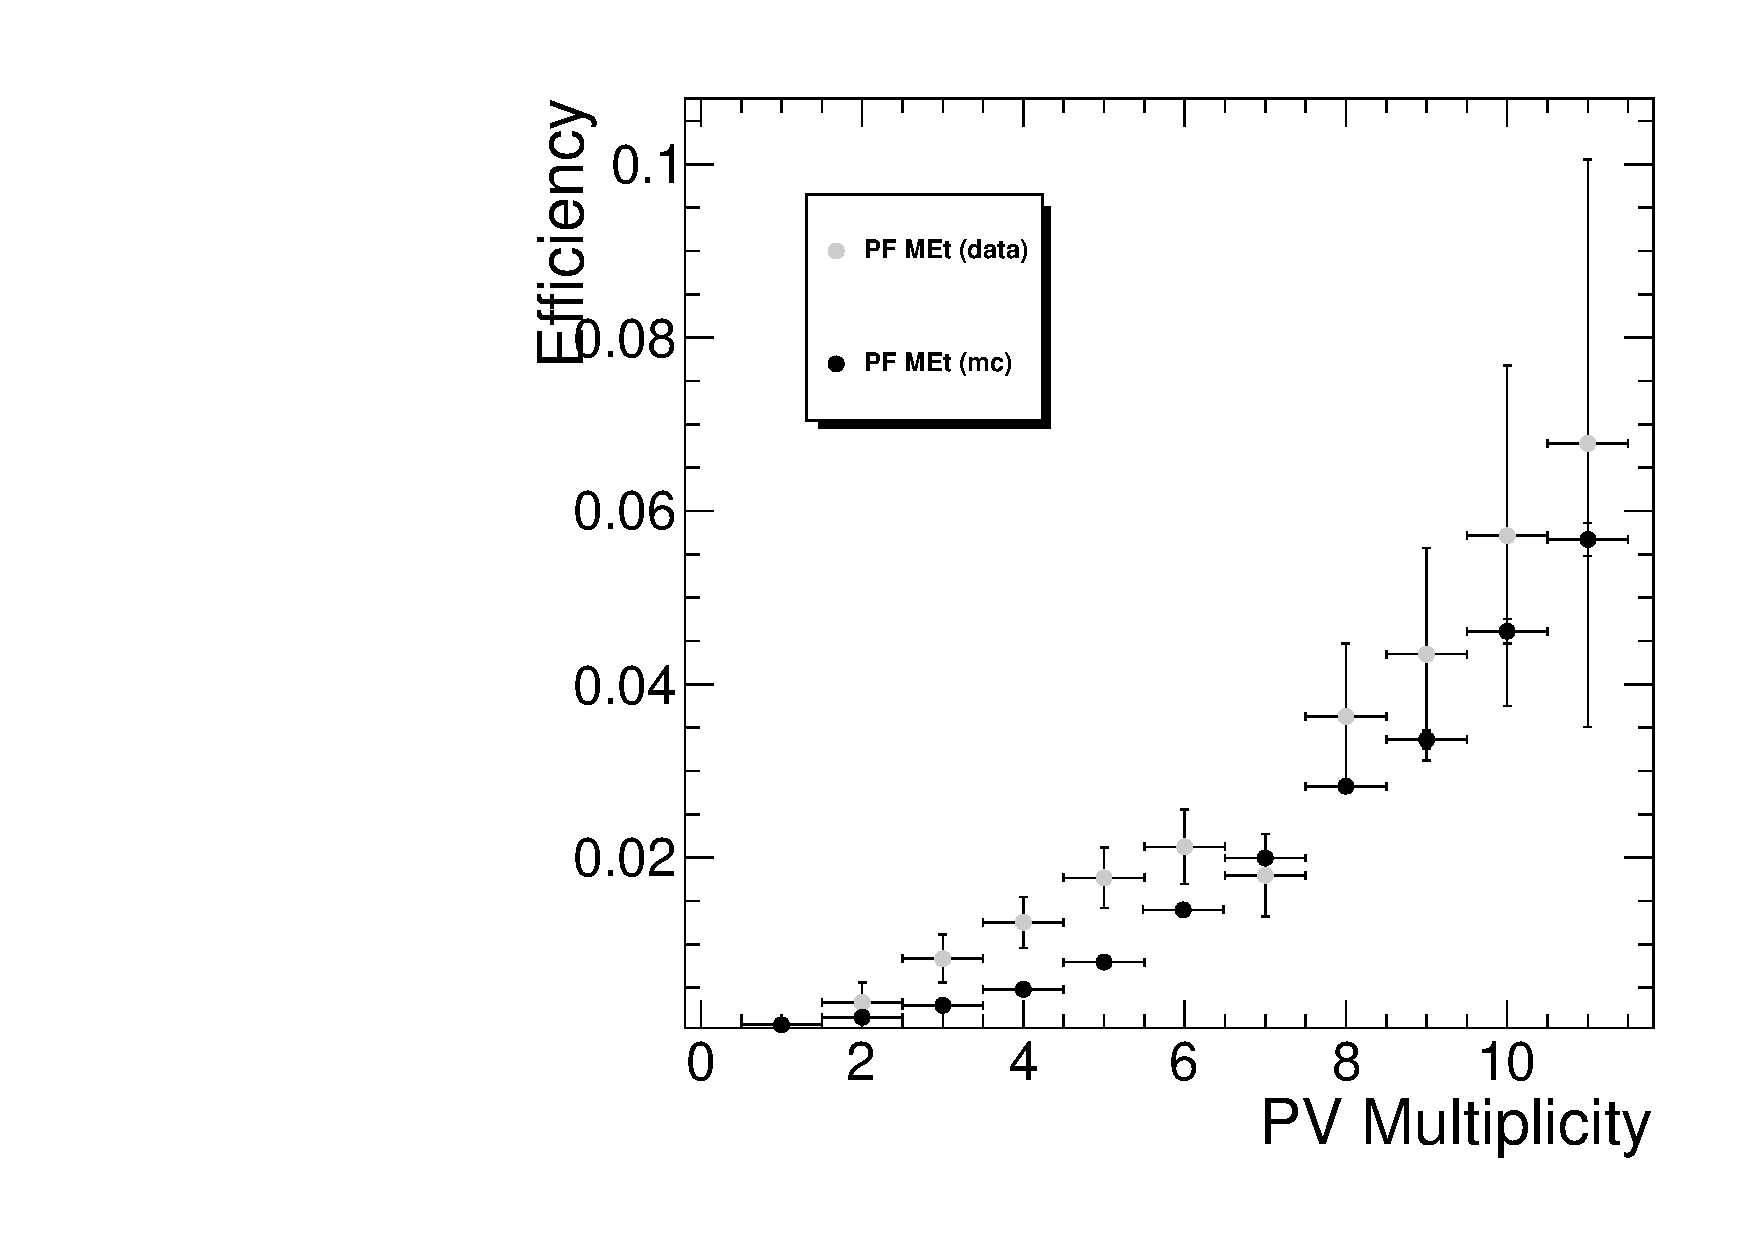
\includegraphics[width=0.3\linewidth]{figures/pfmet_Eff30.pdf} 
\caption{\label{fig:met_pu}\protect Distributions of projected PFMet in data (left) and $\dyll$ MC (center) 
overlayed for low pile-up and high pile-up. The efficiency to satisfy the requirement pfmet$>30$~GeV as a function
of the number of reconstructed vertices in $\dyll$ data and MC.}
\end{center}
%\end{figure}
%%%%%%%%%%%%%%%%%%%%%%%%%%%%%%%%%%%%%%%%%%%
%%%%%%%%%%%%%%%%%%%%%%%%%%%%%%%%%%%%%%%%%%%
%\begin{figure}[hbt]
\begin{center}
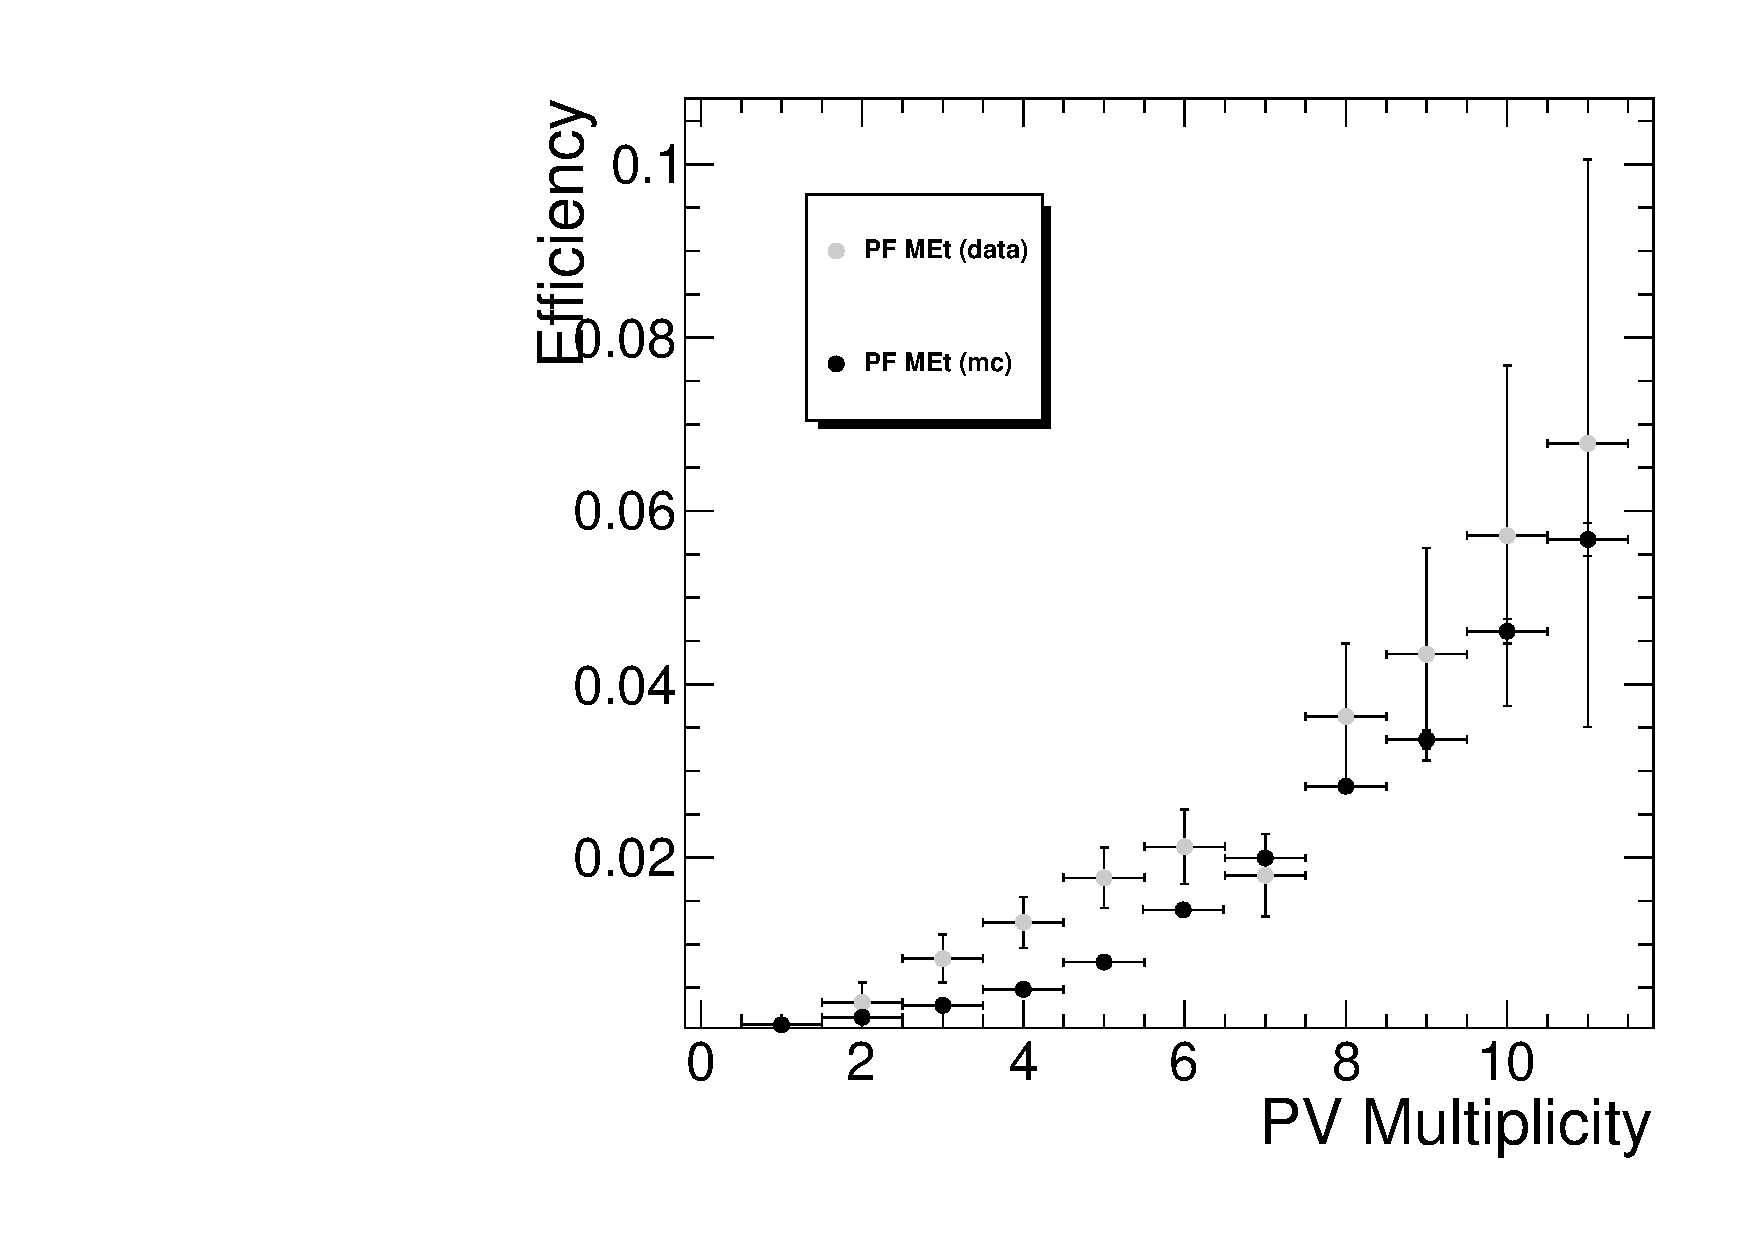
\includegraphics[width=0.5\linewidth]{figures/pfmet_Eff30.pdf} 
\caption{\label{fig:meteff_pu}\protect The efficiency to satisfy the requirement pfmet$>30$~GeV as a function
of the number of reconstructed vertices in $\dyll$ data and MC.}
\end{center}
\end{figure}
%%%%%%%%%%%%%%%%%%%%%%%%%%%%%%%%%%%%%%%%%%%

%%%%%%%%%%%%%%%%%%%%%%%%%%%%%%%%%%%%%%%%%%%
\begin{figure}[hbt]
\begin{center}
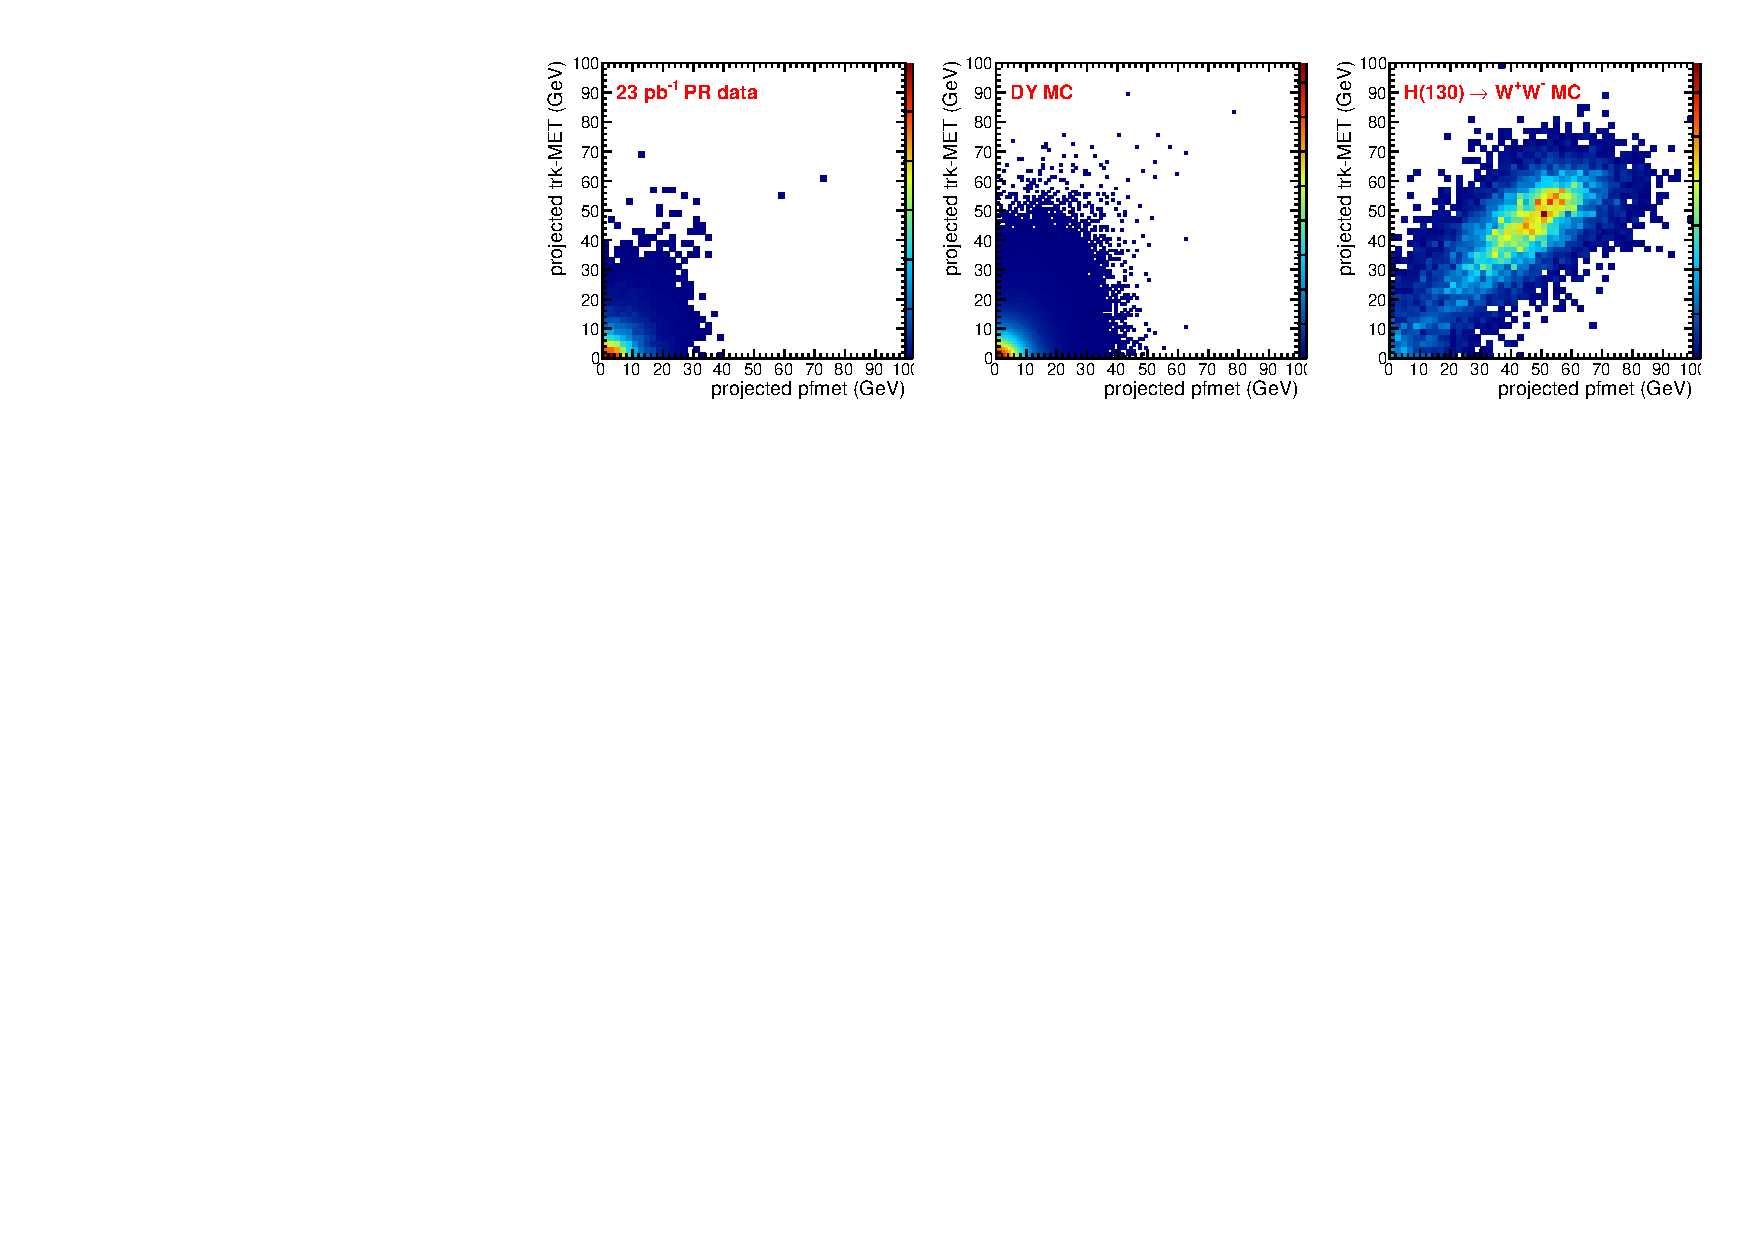
\includegraphics[width=1\linewidth]{figures/met_scatter.pdf} 
\caption{\label{fig:met_scatter}\protect Distributions of trk-MET vs. pfmet in data (left), $\dyll$ MC (center) and Higgs MC (right).}
\end{center}
\end{figure}
%%%%%%%%%%%%%%%%%%%%%%%%%%%%%%%%%%%%%%%%%%%

%%%%%%%%%%%%%%%%%%%%%%%%%%%%%%%%%%%%%%%%%%% 
\begin{figure}[hbt]
\begin{center}
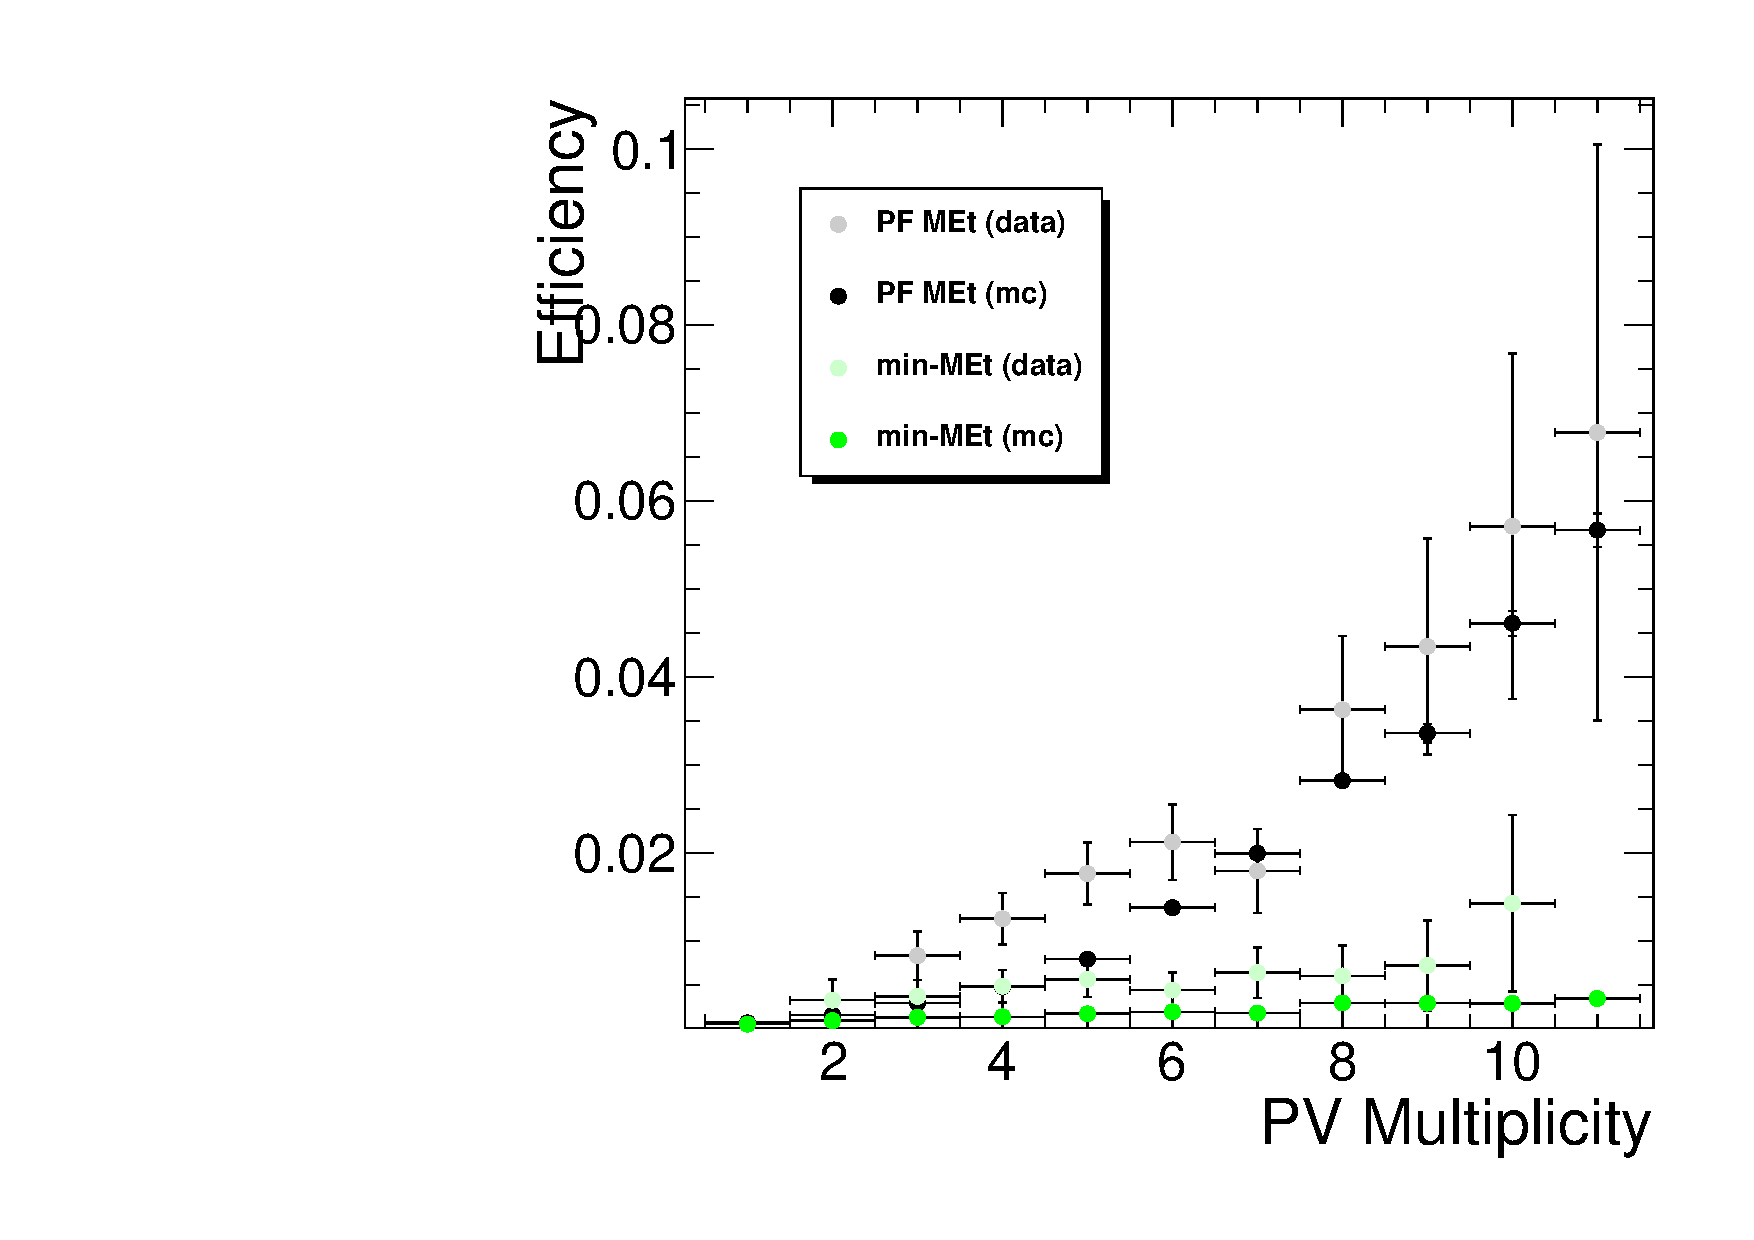
\includegraphics[width=0.45\linewidth]{figures/pfmet_minmet_Eff30.pdf} 
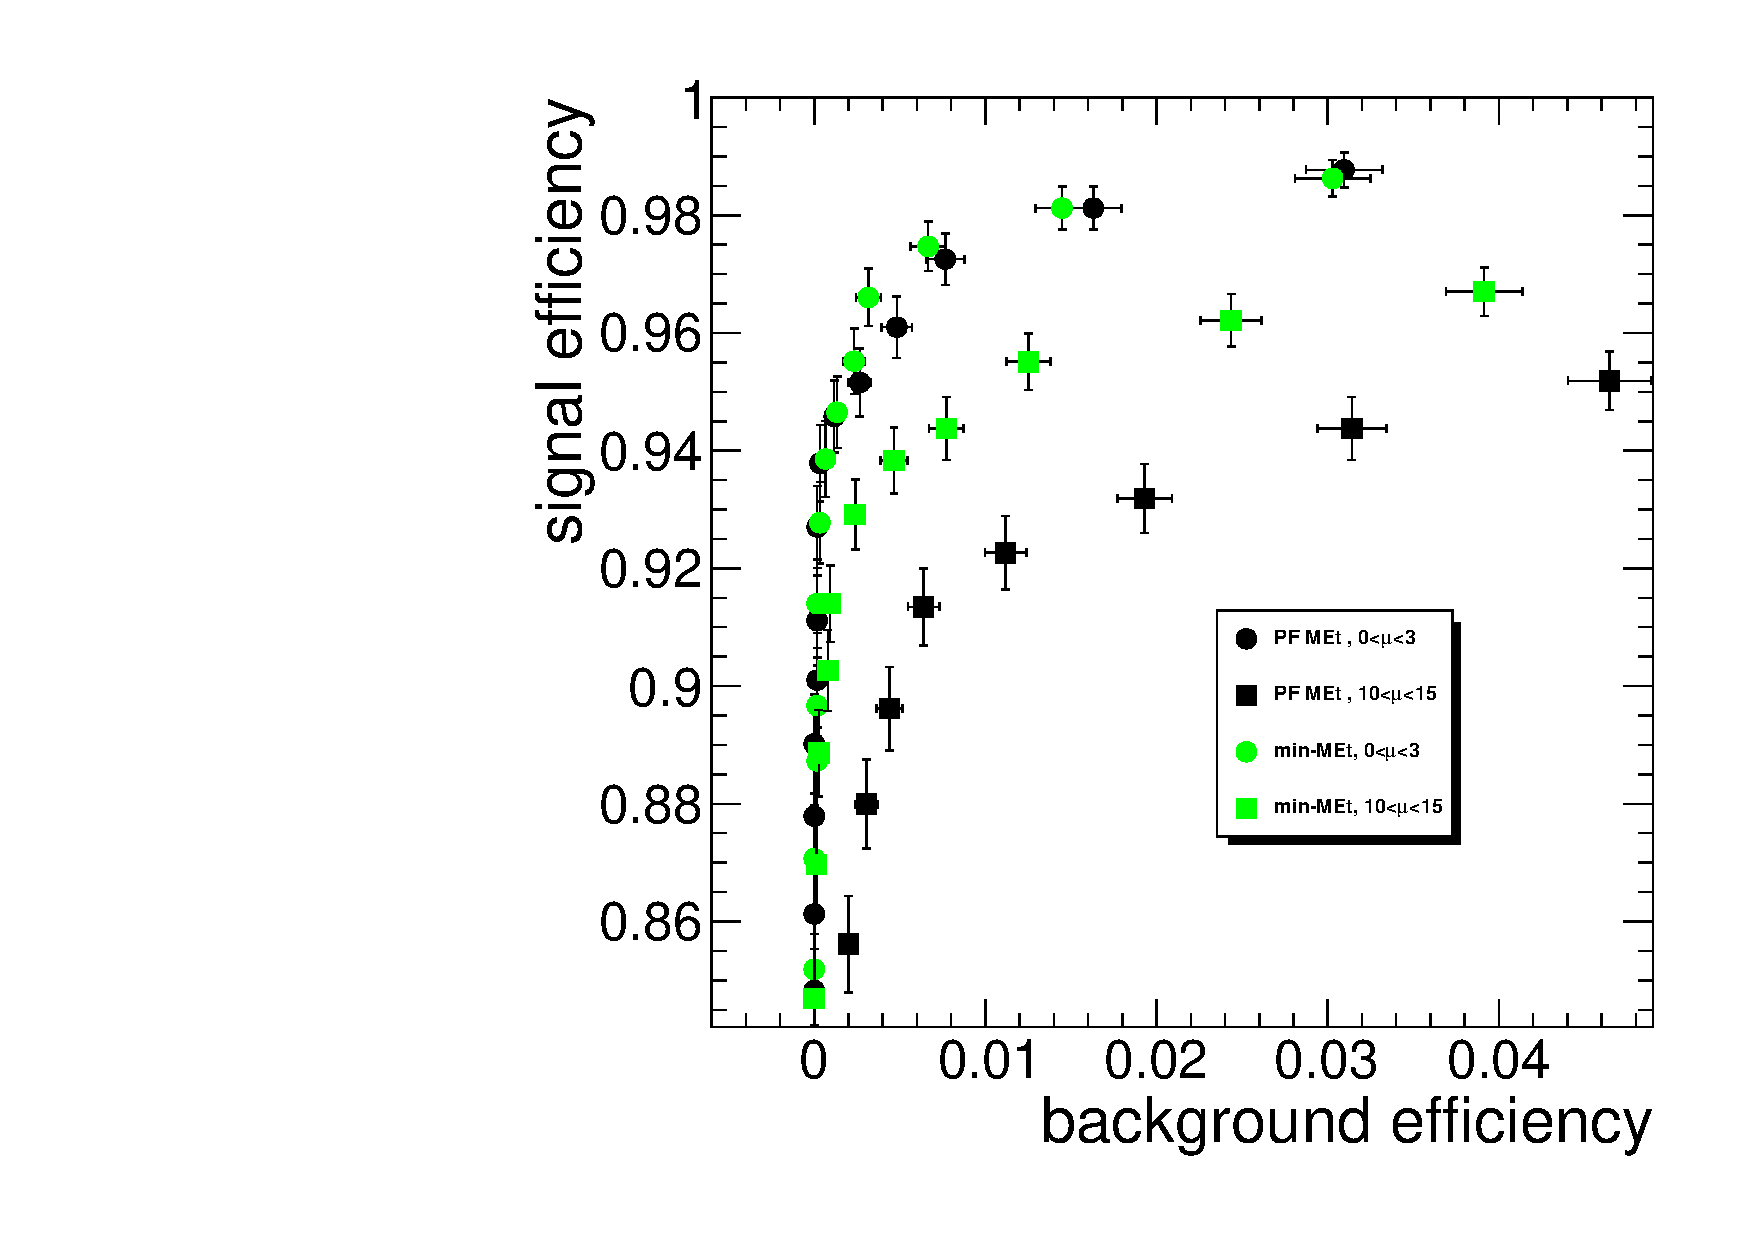
\includegraphics[width=0.45\linewidth]{figures/SignalVsBkgrEfficiency.pdf} 
\caption{\label{fig:met_eff}\protect Left plot shows the efficiency to satisfy
 the requirement pfmet$>$X~GeV as a function of the number of reconstructed 
vertices for Z-events in data and MC. Right plot shows the signal efficiency 
vs. background efficiency, evaluated for H$_{130}$ and $\dyll$ MC.}
\end{center}
\end{figure}
%%%%%%%%%%%%%%%%%%%%%%%%%%%%%%%%%%%%%%%%%%%



%In the presence of high pile-up, the instrumental \met\ tail in $\dyll$ events is enhanced
%significantly, as shown in Figure~\ref{fig:met_pu} for data and $\dyll$ MC. This causes a sharp increase in the
%efficiency for $\dyll$ events to pass a given \met\ requirement as the number of pile-up
%interactions increases. To improve the robustness of the \met\ performance
%in the presence of pile-up, we have developed a novel \met\ algorithm (trk-MET).
%trk-MET is \met\ constructed from charged particles consistent with originating from
%the signal PV. We correct for the 2 leptons, as well as charged PFCandidates which satisfy
%the following requirements:
%\begin{itemize}
%\item the track matched to PFCandidate has $\Delta z < 0.1$~cm with respect to the signal PV;
%\item the signal PV is the closest PV to the track in $\Delta z$;
%\item the track has $\Delta R > 0.1$ with respect to both leptons, to avoid 
%double-counting of the leptons.
%\end{itemize}
%The high \met\ tail in events with no genuine \met\ is larger for trk-MET than for pfmet. However,
%we observe that for data and MC $\dyll$ events these two \met\ flavors are weakly-correlated, as shown
%in Figure~\ref{fig:met_scatter}. Therefore the rejection power for $\dyll$ events is increased significantly
%by cutting on both pfmet and trk-MET, or equivalently by cutting on min-MET $\equiv$ minimum(pfmet,trk-MET).
%In addition, the high \met\ tail efficiency vs. number of pile-up interactions is flattened, as shown
%in Figure~\ref{fig:met_eff}. For signals with genuine \met\, trk-MET and pfmet are strongly correlated. 
%The signal (H(130) MC) efficiency vs. background ($\dyll$ MC) efficiency is shown in 
%Figure~\ref{fig:met_eff} for min-MET and pfmet.

   \subsection{Jet Counting} 
     \label{sec:sel_jets}
     %To split the analysis in different jet bins, we count events 
%containing jets with $\pt > ~30~\GeV$ within $|\eta|<5.0$. 

We analyze the events separately based on the number of reconstructed 
jets with $\pt > ~30~\GeV$ within $|\eta|<5.0$ in the event. 
Jets are reconstructed using calorimeter and tracker information using a particle flow 
algorithm~\cite{jetpas}. The anti-${\rm k_T}$ clustering algorithm~\cite{antikt} 
with ${\rm R=0.5}$ is used. We apply the standard jet energy 
corrections~\cite{jes} to the reconstructed jets, where the L1 Fast Jets 
corrections are included. The latter corrections are rather important since 
they help in flatening the reconstruction efficiency as a function of the 
number of overlapping events.
To exclude electrons and muons from the jet sample, these 
jets are required to be separated from the selected leptons in $\Delta R$ 
by at least $\Delta R^{\mathrm{jet-lepton}}>0.3$.

%In the 0-Jet bin, the performance of the jet veto 
%is validated on data using Drell-Yan events, 
%as will be explained in Sec.~\ref{sec:backgrounds}. 

  \subsection{Top Tagging}
     \label{sec:sel_toptag}
     
Since the top quark production cross-section is substantially higher than the
diboson production cross-section, top backgrounds generally pose a significant 
challenge for dilepton plus \met analyses. To reduce the top background, 
we use a combination of two top tagging methods implemented and commissioned in the $\hww$ 
analysis~\cite{HWW2011AN}, both relying on the fact that top quarks 
decay to $Wb$ with almost certainty.

The first method vetoes events containing soft muons from the $b$-quark decays 
The requirements used to select soft muons are:
%%%%%%%%%%%%
\begin{itemize}
    \item $\pt > 3$ GeV;
    \item Reconstructed as a TrackerMuon
    \item Meets $\mathrm{TMLastStationAngTight}$ muon id requirements
    \item The number of valid inner tracker hits $>10$
    \item The transverse impact parameter with respect to the Primary Vertex, $|d_{0}| < 0.2$~cm,
    \item The longitudinal impact parameter with respect to the Primary Vertex, $|d_{z}| < 0.2$~cm,
    \item Non-isolated $({\rm{Iso}_{Total}}/{\pt}~>~0.1)$ if $\pt>20\GeV$.
\end{itemize}
%%%%%%%%%%%%

The second method uses standard $b$-jet tagging. 
The jets are reconstructed using calorimeter and tracker information using a particle flow 
algorithm~\cite{jetpas}. The anti-${\rm k_T}$ clustering algorithm~\cite{antikt} 
with ${\rm R=0.5}$ is used. We apply the standard jet energy 
corrections~\cite{jes} to the reconstructed jets, where the L1 Fast Jets 
corrections are included. The latter corrections are rather important since 
they help in flatening the reconstruction efficiency as a function of the 
number of overlapping events.
In this method, events containing jets with $E_T>30\GeV$ tagged with
 the $\mathrm{TrkCountingHighEff}$~\cite{btag} algorithm with
a discriminator value of greater than 2.0 are vetoed. 
	

%The algorithm is applied to jets with the same definition as Section \ref{sec:sel_jets},
%with the exception that the $E_T$ requirement is removed. 
%Thus, events in the zero-jet bin can still contain tagged jets.

%As a comparison of performance , the $\WW$ signal efficiency versus the $\ttbar$ efficiency in 
%events with no jets according to the definition in Section \ref{sec:sel_jets} for different 
%standard b-tagging algorithms  is shown in Figure~\ref{fig:eff_btag_tt_ww}. 
%For a top rejection efficiency above $40\%$,
%the $\mathrm{TrkCountingHighEff}$ tagger performs better than the others.
%Our current cut value has a $\WW$ signal efficiency of about $98.1\%$ and
%a $\ttbar$ efficiency of about $39\%$.

%%%%%%%%%%%%
%\begin{figure}[!htbp]
%\begin{center}
%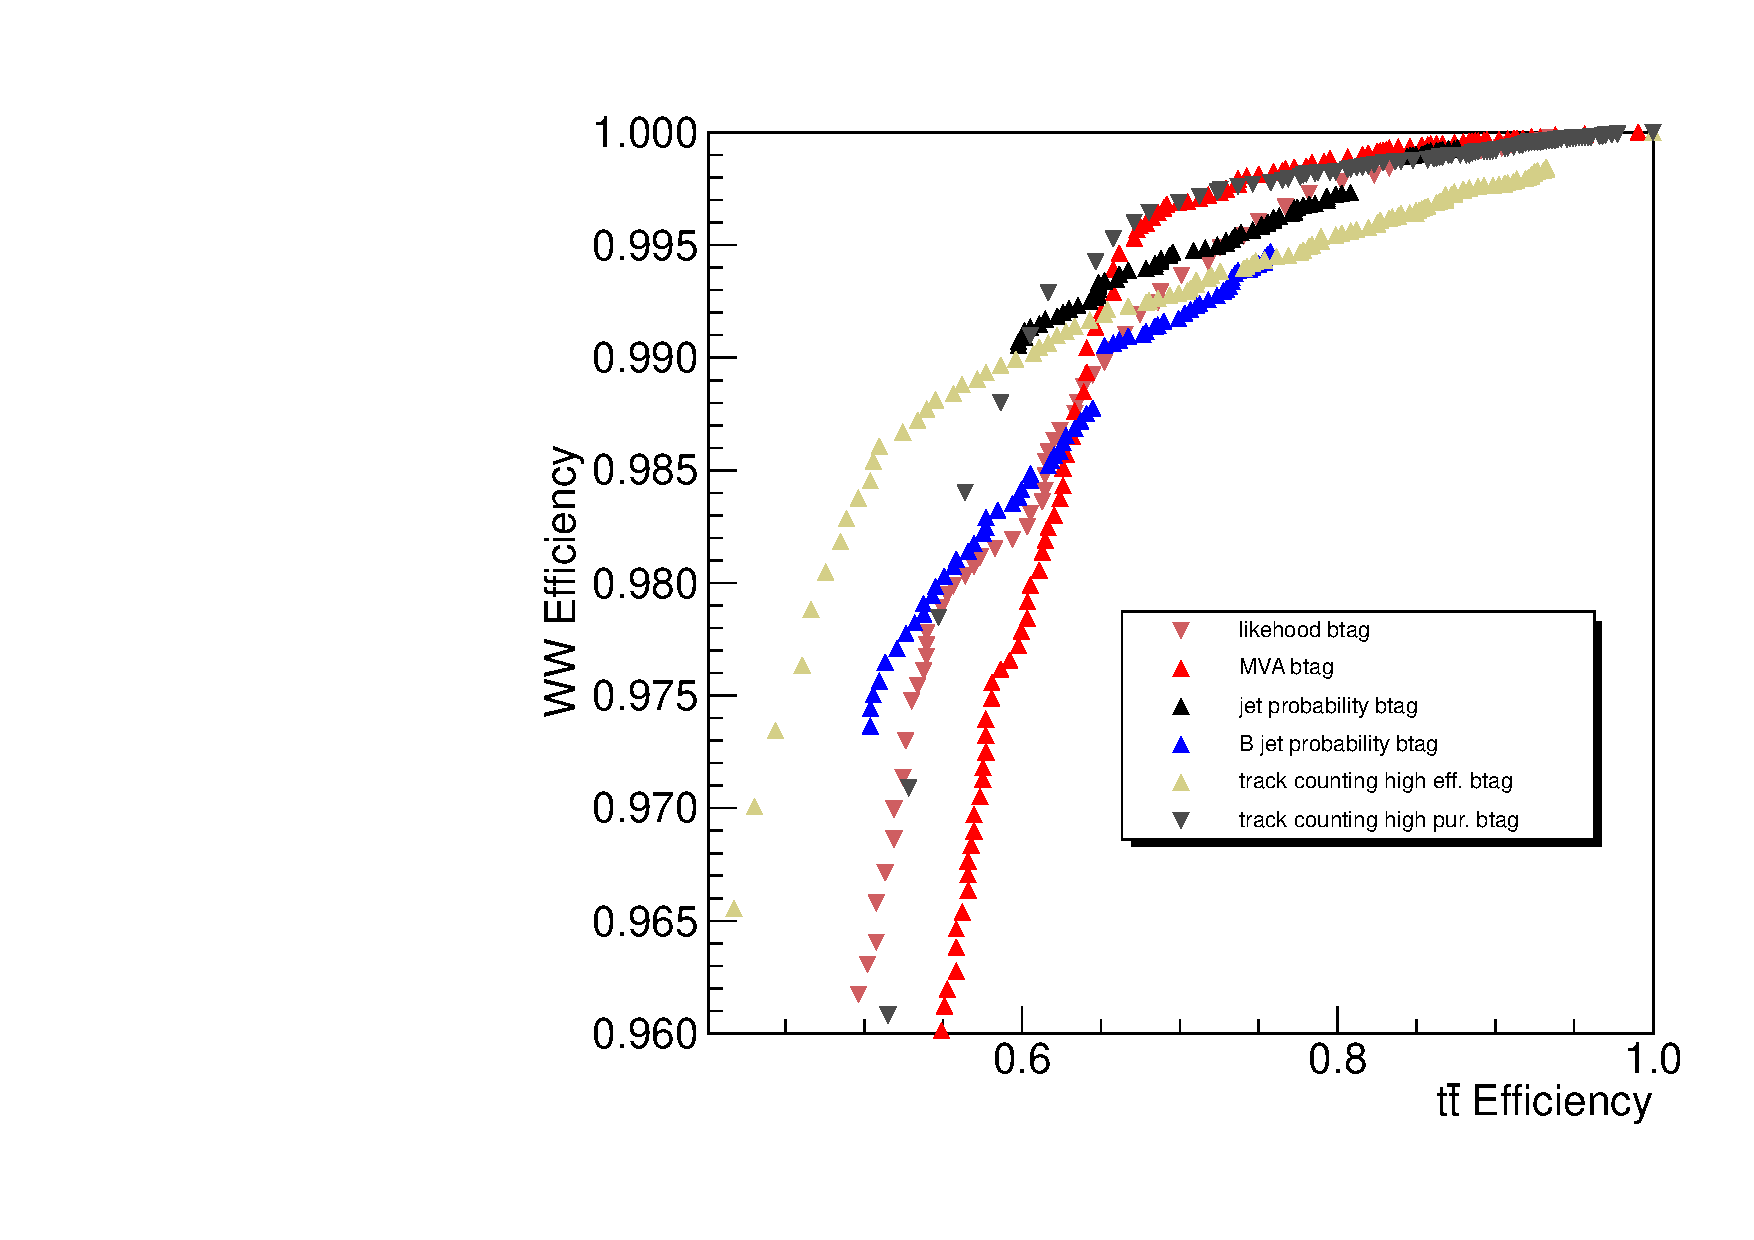
\includegraphics[width=0.60\textwidth]{figures/eff_btag_tt_ww.pdf}
%\caption{$\WW$ signal efficiency versus $\ttbar$ efficiency in events with no
%reconstructed jets for different standard b-tagging algorithms.}
%\label{fig:eff_btag_tt_ww}
%\end{center}
%\end{figure}
%%%%%%%%%%%%

%By using the expected tagging efficiency for the two methods,
%it is possible to estimate the residual top background after the vetoes
%have been applied. 
%This is described in detail in Section \ref{sec:bkg_top}.

   \subsection{Third Lepton Veto}
     \label{sec:sel_lepveto}
     To reduce the background from diboson processes, we veto events
containing an additional lepton meeting the previously described
selection requirements with $\pt > 10~\GeV$.  This removes $\sim
60\%$ of the $WZ$ component and $\sim 10\%$ of the $ZZ$ one.  The \ZZ\
component is dominated by $\ZZ \to 2l2\nu$ decays. The efficiency for
$WW \to 2l2\nu$ events is $\sim 99.9\%$.  

   \subsection{Other Preselection Requirements}
     \label{sec:sel_other}
     To reduce the background from diboson processes, we veto events
containing an additional lepton meeting the previously described
selection requirements with $\pt > 10~\GeV$.  This removes $\sim
60\%$ of the $WZ$ component and $\sim 10\%$ of the $ZZ$ one.  The \ZZ\
component is dominated by $\ZZ \to 2l2\nu$ decays. The efficiency for
$WW \to 2l2\nu$ events is $\sim 99.9\%$.  Finally, in the events 
containing 2 or more jets, the angle in the transverse plane between 
the dilepton system and the system of two most energetic jets with 
$\pt^{jet}~>~15~\GeV$ must be smaller than $165$ degrees in
the $ee/\mu\mu$ final states. This requirement rejects $\dyll$
events, where the $\Z$ boson recoil against jets.
In the events with 0 or 1 jets, this variable is used as an input 
to the MVA-based Drell-Yan suppression technique.


   \subsection{Selection for Same-Flavor Final State}
     \label{sec:sel_sf}
     To further reduce the Drell--Yan background, in the $\Ep\Em$ and
$\Mp\Mm$ final states we apply a few additional cuts.

First, to avoid the peaking component of \dyll, we veto events with a dilepton invariant mass within $15~\GeV$ of the $\Z$.  
Then, depending on the jet bin and the Higgs mass hypothesis, different approaches are exploited.

In the 0 and 1 jet final states, a MVA-based Drell-Yan suppression techique~\cite{dymva} (DY MVA) is used; 
DY MVA combines information from variables related to missing energy, kinematic and topological variables
maximising the signal-to-background ratio.

%For the high Higgs mass and $\WW$ analyses containing less than two jets, the signal has larger \met\ and
%the \dyll\ background is less important; therefore, a multivariate approach does not improve the performance and 
%min-MET is used as a discrimiating variable. 
%In addition, in order to reject events where the $\Z$ boson recoils against jets, the angle in 
%the transverse plane between the dilepton system and the most energetic jet with $\pt^{jet}~>~15~\GeV$ 
%must be smaller than $165$ degrees.

In events with two or more jets, pileup effects are not dominant since fake \met\ in \dyll\ is mainly due to the mismeasurement of 
the hadronic recoil; therefore, the use of track-MET degradres the performance and plain pf-MET is used. 
In this case, the hadronic recoil is clustered into two jets; thus, the system of the two most energetic jets is considered when cutting 
on the azimuthal angle difference from the dilepton momentum.

The selection requirements are summarized in Table~\ref{tab:metsel}.  

\begin{table}[htp]
\centering
\setlength{\tabcolsep}{15pt}
\begin{tabular}{|c|c|c|c|}
\hline 
variable 	 & 0-jet & 1-jet & 2-jet \\
\hline \hline 
DY MVA		 & $>$0.88 & $>$0.84 & - \\
pfMet            &  -  & - & $>$45 \GeV\ \\
$\Delta\phi$(\Lep\Lep,jj)  & - & - & $<$165$^\circ$ \\
\hline \hline 
$|$\mll\ - $m_\Z$$|$  & \multicolumn{3}{|c|}{$>$15 \GeV} \\
\hline 
\end{tabular}
\caption{Selection cuts specific for same-flavor final states. }
\label{tab:metsel}
\end{table}


\section{Higgs Signal Extraction Strategy}
   To enhance the sensitivity to the Higgs boson signal, two different approaches 
are performed. The first one is a cut-based approach where further requirements 
on a few observables are applied, while the second one makes use of
multivariate techniques. Both of them cover a large Higgs boson mass
($m_{\rm{H}}$) range, and each is separately optimized for different
$m_{\rm{H}}$ hypotheses. The first method is the simplest approach to
be performed on the limited recorded data sample. The second one is
more powerful, since it exploits the information present in the
correlation among the variables. All analyses are further split in 
the corresponding 0-jet, 1-jet and 2-jet bins. Due to the limited 
sensitivity in the 2-jet bin and the little amount of simulated events, 
we decided to have a simple cut-based approach only for now.

   \label{sec:signal_selection}
   \subsection{Cut Based Analysis}
     \label{sec:anal_cutbased}
    \subsubsection{0/1-Jet Selection}
      \label{sec:sel_zerojet}
      After the $\WW$ selection, the following handles are used to discriminate
against the remaining background, specially $\WW$ continuum:

\begin{itemize}
\item the angle $\delphill$ between the two selected leptons in the transverse 
plane. This variable provides the best discriminating 
power between the Higgs signal and the majority of the backgrounds for 
$\hww$ production in the low Higgs boson mass range. Leptons originating from 
$\hww$ decays tend to have a relatively small opening angle, while those from 
backgrounds are preferentially emitted back-to-back. The importance of this 
variable decreases for high masses, since the boost of the $\W$ bosons 
dilutes the angular correlation;

\item an upper cut on the invariant mass of the lepton-pair;

\item a lower cut on the transverse momenta of the harder (\ptlmax) and 
the softer (\ptlmin) lepton;

\item the transverse Higgs mass, $m_{T}^{\ell\ell\met} = \sqrt{2\pt^{ll}\met(1-cos(\ell\ell-\met))}$.

\end{itemize} 

As a reference we use 2010 analysis cut based approach documented
in~\cite{HWW2010}. Table~\ref{tab:cutanalysis0j} summarizes selection
requirements re-tuned for this analysis.

\begin{table}[!ht]
  \begin{center}
 {\small
  \begin{tabular} {|c|c|c|c|c|c|c|}
  \hline
\mHi [GeV] & $\ptlmax$ [$\GeV$] & $\ptlmin$ [$\GeV$] & $\mll$ [$\GeV$] & $\delphill$ [dg.] & $m_{T}^{\ell\ell\met}$ [GeV  \\  \hline
           &   $>$               &   $>$               &   $<$             &  $<$          &    [,]                       \\  \hline

  \hline
  \hline
  H$_{120}$ & 20 & 10 & 2.0 & 40 & [70,120]\\
  H$_{130}$ & 25 & 10 & 1.5 & 45 & [75,125]\\
  H$_{140}$ & 25 & 15 & 1.5 & 45 & [80,130]\\
  H$_{150}$ & 27 & 25 & 1.5 & 50 & [80,150]\\
  H$_{160}$ & 30 & 25 & 1.0 & 50 & [90,160]\\
  \hline
 \hline
  \end{tabular}
  }
  \caption{Final Event selection requirements for a cut-based analysis}
   \label{tab:cutanalysis0j}
  \end{center}
\end{table}


\begin{table}[!ht]
  \begin{center}
 {\small
  \begin{tabular} {|c|c|c|c|}
  \hline
  Mass   &  R(2020) & R(2010) & R(new) \\
  \hline
  \hline
  H$_{120}$ & 7.6 & 5.0 & 3.4 \\
  H$_{130}$ & 2.7 & 2.3 & 1.7 \\
  H$_{140}$ & 1.4 & 1.4 & 1.2 \\
  H$_{150}$ & 0.88 & 0.93 & 0.80 \\
  H$_{160}$ & 0.44 & 0.60 & 0.43 \\
  \hline


 \hline
  \end{tabular}
  }
  \caption{Cut based analysis performance for different tunes. R(2020) refers 
  to 2010 analysis with minimum lepton \pt\ of 20 GeV. R(2010) is the same set of cuts,
  but the trailing lepton \pt\ is lowered to 10 GeV for Higgs mass hypothesis 
  of 160 GeV and lower. R(new) is a new set of cuts used in this analysis.}
   \label{tab:cutanalysis_perf}
  \end{center}
\end{table}


\begin{table}[!ht]
  \begin{center}
 {\footnotesize
  \begin{tabular} {|c|c|c|c|c|c|c|c|c||c||c|}
\hline
  & DY & ttbar & TW & Wjets & WZ & ZZ & ggWW & qqWW & {\bf All bkg} & {\bf H$_{120}$}\\
  \hline
  \hline
  mm &  0.8$\pm$0.8 &  0.4$\pm$0.3 &  0.3$\pm$0.1 &  4.4$\pm$3.1 &  0.3$\pm$0.1 &  0.5$\pm$0.0 &  0.6$\pm$0.0 & 12.9$\pm$0.3 & 20.2$\pm$3.2 & 2.5$\pm$0.1 \\
  me &  0.0$\pm$0.0 &  0.7$\pm$0.3 &  0.3$\pm$0.1 &  4.4$\pm$3.1 &  0.3$\pm$0.0 &  0.0$\pm$0.0 &  0.4$\pm$0.0 &  8.4$\pm$0.2 & 14.4$\pm$3.1 & 1.5$\pm$0.0 \\
  em &  0.0$\pm$0.0 &  0.6$\pm$0.3 &  0.4$\pm$0.1 &  6.4$\pm$3.7 &  0.4$\pm$0.1 &  0.0$\pm$0.0 &  0.5$\pm$0.0 & 11.7$\pm$0.3 & 20.1$\pm$3.7 & 2.5$\pm$0.1 \\
  ee &  0.0$\pm$0.0 &  0.1$\pm$0.1 &  0.1$\pm$0.1 &  6.2$\pm$3.6 &  0.2$\pm$0.0 &  0.2$\pm$0.0 &  0.3$\pm$0.0 &  6.1$\pm$0.2 & 13.2$\pm$3.6 & 1.1$\pm$0.0 \\
 \hline
 all &  0.8$\pm$0.8 &  1.9$\pm$0.5 &  1.1$\pm$0.2 & 21.3$\pm$6.7 &  1.2$\pm$0.1 &  0.8$\pm$0.0 &  1.8$\pm$0.1 & 39.0$\pm$0.5 & 67.9$\pm$6.8 & 7.6$\pm$0.1 \\
 \hline
  \end{tabular}
  }
 {\footnotesize
  \begin{tabular} {|c|c|c|c|c|c|c|c|c||c||c|}
\hline
  & DY & ttbar & TW & Wjets & WZ & ZZ & ggWW & qqWW & {\bf All bkg} & {\bf H$_{130}$}\\
  \hline
  \hline
  mm & 0.8$\pm$0.8 &  0.3$\pm$0.2 &  0.3$\pm$0.1 &  4.4$\pm$3.1 &  0.4$\pm$0.1 &  0.5$\pm$0.0 &  0.7$\pm$0.0 & 14.5$\pm$0.3 & 21.8$\pm$3.2 & 4.9$\pm$0.1 \\
  me & 0.0$\pm$0.0 &  1.0$\pm$0.4 &  0.3$\pm$0.1 &  2.2$\pm$2.2 &  0.3$\pm$0.0 &  0.0$\pm$0.0 &  0.5$\pm$0.0 &  9.2$\pm$0.2 & 13.4$\pm$2.2 & 3.2$\pm$0.1 \\
  em & 0.0$\pm$0.0 &  0.4$\pm$0.3 &  0.5$\pm$0.1 &  2.1$\pm$2.1 &  0.4$\pm$0.1 &  0.0$\pm$0.0 &  0.6$\pm$0.0 & 12.3$\pm$0.3 & 16.3$\pm$2.1 & 4.4$\pm$0.1 \\
  ee & 0.8$\pm$0.8 &  0.1$\pm$0.1 &  0.1$\pm$0.0 &  8.2$\pm$4.1 &  0.2$\pm$0.0 &  0.2$\pm$0.0 &  0.4$\pm$0.0 &  7.1$\pm$0.2 & 17.2$\pm$4.2 & 2.4$\pm$0.1 \\
 \hline
 all & 1.6$\pm$1.1 &  1.9$\pm$0.5 &  1.2$\pm$0.2 & 16.8$\pm$5.9 &  1.2$\pm$0.1 &  0.7$\pm$0.0 &  2.2$\pm$0.1 & 43.1$\pm$0.5 & 68.9$\pm$6.1 & 15.0$\pm$0.2 \\
 \hline
  \end{tabular}
  }
 {\footnotesize
  \begin{tabular} {|c|c|c|c|c|c|c|c|c||c||c|}
\hline
  & DY & ttbar & TW & Wjets & WZ & ZZ & ggWW & qqWW & {\bf All bkg} & {\bf H$_{140}$}\\
  \hline
  \hline
  mm & 0.8$\pm$0.8 &  0.3$\pm$0.2 &  0.3$\pm$0.1 &  2.2$\pm$2.2 &  0.3$\pm$0.0 &  0.4$\pm$0.0 &  0.7$\pm$0.0 & 13.1$\pm$0.3 & 18.1$\pm$2.4 & 6.3$\pm$0.1 \\
  me & 0.0$\pm$0.0 &  1.0$\pm$0.4 &  0.3$\pm$0.1 &  2.2$\pm$2.2 &  0.3$\pm$0.0 &  0.0$\pm$0.0 &  0.5$\pm$0.0 &  9.5$\pm$0.2 & 13.9$\pm$2.2 & 5.1$\pm$0.1 \\
  em & 0.0$\pm$0.0 &  0.3$\pm$0.2 &  0.3$\pm$0.1 &  0.0$\pm$0.0 &  0.3$\pm$0.1 &  0.0$\pm$0.0 &  0.6$\pm$0.0 & 10.8$\pm$0.3 & 12.4$\pm$0.3 & 5.6$\pm$0.1 \\
  ee & 0.8$\pm$0.8 &  0.1$\pm$0.1 &  0.2$\pm$0.1 &  8.2$\pm$4.1 &  0.2$\pm$0.0 &  0.2$\pm$0.0 &  0.5$\pm$0.0 &  7.6$\pm$0.2 & 17.8$\pm$4.2 & 4.1$\pm$0.1 \\
 \hline
 all & 1.6$\pm$1.1 &  1.8$\pm$0.5 &  1.2$\pm$0.2 & 12.6$\pm$5.1 &  1.1$\pm$0.1 &  0.6$\pm$0.0 &  2.3$\pm$0.1 & 41.0$\pm$0.5 & 62.1$\pm$5.3 & 21.2$\pm$0.2 \\
 \hline
  \end{tabular}
  }
 {\footnotesize
  \begin{tabular} {|c|c|c|c|c|c|c|c|c||c||c|}
\hline
  & DY & ttbar & TW & Wjets & WZ & ZZ & ggWW & qqWW & {\bf All bkg} & {\bf H$_{150}$}\\
  \hline
  \hline
  mm & 0.8$\pm$0.8 &  0.4$\pm$0.3 &  0.1$\pm$0.1 &  0.0$\pm$0.0 &  0.3$\pm$0.1 &  0.2$\pm$0.0 &  0.6$\pm$0.0 &  8.1$\pm$0.2 & 10.5$\pm$0.9 & 6.5$\pm$0.1 \\
  me & 0.0$\pm$0.0 &  0.6$\pm$0.3 &  0.3$\pm$0.1 &  0.0$\pm$0.0 &  0.2$\pm$0.0 &  0.0$\pm$0.0 &  0.5$\pm$0.0 &  6.4$\pm$0.2 &  8.0$\pm$0.4 & 5.3$\pm$0.1 \\
  em & 0.0$\pm$0.0 &  0.4$\pm$0.3 &  0.3$\pm$0.1 &  0.0$\pm$0.0 &  0.2$\pm$0.0 &  0.0$\pm$0.0 &  0.5$\pm$0.0 &  6.9$\pm$0.2 &  8.4$\pm$0.3 & 5.4$\pm$0.1 \\
  ee & 0.0$\pm$0.0 &  0.3$\pm$0.2 &  0.1$\pm$0.0 &  2.1$\pm$2.1 &  0.1$\pm$0.0 &  0.1$\pm$0.0 &  0.4$\pm$0.0 &  5.2$\pm$0.2 &  8.3$\pm$2.1 & 4.3$\pm$0.1 \\
 \hline
 all & 0.8$\pm$0.8 &  1.8$\pm$0.5 &  0.8$\pm$0.1 &  2.1$\pm$2.1 &  0.7$\pm$0.1 &  0.3$\pm$0.0 &  2.1$\pm$0.1 & 26.6$\pm$0.4 & 35.2$\pm$2.3 & 21.5$\pm$0.3 \\
 \hline
  \end{tabular}
  }
 {\footnotesize
  \begin{tabular} {|c|c|c|c|c|c|c|c|c||c||c|}
\hline
  & DY & ttbar & TW & Wjets & WZ & ZZ & ggWW & qqWW & {\bf All bkg} & {\bf H$_{160}$}\\
  \hline
  \hline
  mm & 0.0$\pm$0.0 &  0.4$\pm$0.3 &  0.1$\pm$0.1 &  0.0$\pm$0.0 &  0.2$\pm$0.0 &  0.1$\pm$0.0 &  0.5$\pm$0.0 &  5.2$\pm$0.2 &  6.6$\pm$0.3 & 8.9$\pm$0.2 \\
  me & 0.0$\pm$0.0 &  0.3$\pm$0.2 &  0.2$\pm$0.1 &  0.0$\pm$0.0 &  0.1$\pm$0.0 &  0.0$\pm$0.0 &  0.5$\pm$0.0 &  4.2$\pm$0.2 &  5.3$\pm$0.3 & 8.0$\pm$0.2 \\
  em & 0.0$\pm$0.0 &  0.3$\pm$0.2 &  0.3$\pm$0.1 &  0.0$\pm$0.0 &  0.1$\pm$0.0 &  0.0$\pm$0.0 &  0.5$\pm$0.0 &  4.5$\pm$0.2 &  5.7$\pm$0.3 & 7.8$\pm$0.2 \\
  ee & 0.0$\pm$0.0 &  0.3$\pm$0.2 &  0.1$\pm$0.0 &  0.0$\pm$0.0 &  0.1$\pm$0.0 &  0.1$\pm$0.0 &  0.4$\pm$0.0 &  3.5$\pm$0.1 &  4.3$\pm$0.3 & 6.1$\pm$0.1 \\
 \hline
 all & 0.0$\pm$0.0 &  1.3$\pm$0.4 &  0.7$\pm$0.1 &  0.0$\pm$0.0 &  0.6$\pm$0.1 &  0.2$\pm$0.0 &  1.8$\pm$0.1 & 17.3$\pm$0.3 & 21.9$\pm$0.6 & 30.9$\pm$0.3 \\
 \hline
  \end{tabular}
  }
  \caption{Expected number of signal and background events for an 
  integrated luminosity of 1\ifb{} after 
  applying the full cut-based 0-jet selection requirements. Monte Carlo statistical uncertainties are 
  included.}
   \label{tab:cutbase_yeilds}
  \end{center}
\end{table}


     \subsubsection{VBF Selection}
       \label{sec:sel_vbf}
       The cross section for Higgs boson production in the vector boson fusion (VBF)
mode is roughly ten times smaller than the gluon-gluon fusion mode.
However, the VBF signal can be extracted
using simple selections, especially in the fully leptonic decay channel
where the backgrounds are expected to be relatively low.

The $\hww$ events from VBF production is characterized by a pair of energetic 
forward-backward jets and very little hadronic activity in the rest of the event. 
As a starting point, we select the events that pass the $\ww$ preselection 
requiring two reconstructed jets with $\pt~>~30~\GeV$ and no other jets between 
them with $\pt~>~30~\GeV$. To reject the main background from top decays we 
apply further selections on the two jets $j_1$ and $j_2$:
\begin{itemize}
  \item neither of the jets must be $b$-tagged;
  \item $\Delta\eta (j_1-j_2) > 3.5$;
  \item $m_{j_1j_2} > 450\:\GeV$;
  \item $30~\GeV < m_{T}^{\ell\ell\met} < m_H~\GeV$.
\end{itemize}
To improve the selection efficiency signal we select 
events with a $\mHi$ dependent requirement on the high end of the dilepton mass 
(the actual cut value is the same as in the MVA analysis, 
see Sec.~\ref{sec:anal_mva}, Table~\ref{tab:presel_tmva_analysis}). 
Events with same and opposite flavor final states 
are separated in order to obtain better sensitivity in the final limit.   
The $qqH$ contribution to the total  $\hww$ signal is found to be about 85\%
after full event selections for all the mass hypotheses considered. 

   \subsection{MVA Analysis}
     \label{sec:anal_mva}
     To make maximal use of the event information we have performed a multivariate analysis 
using a multivariate classifier based on the Boosted Decision Tree (BDT) technique. 
The BDT is implemented using the TMVA~\cite{tmva} toolkit and has been 
successfully applied in high energy physics to increase the 
statistical significance of a signal extraction
It requires less training than other multivariate classifiers and 
it is insensitive to the inclusion of poorly discriminating input variables.

In addition to the $\WW$ preselection, we apply a loose cut on the
maximum $\mll$ to enhance the signal-to-background ratio shown in 
Table~\ref{tab:presel_tmva_analysis} and a cut on $\mt$: (80-$\mHi$) $\GeV$ to 
supress the $\dytt$ and $wgamma$ backgrounds. 
In addition to the selection variables for the cut-based analysis, the multivariate signal extraction 
procedure uses the following ones: 
\begin{itemize}
\item $\Delta R_{\Lep\Lep}\equiv\sqrt{\deletall^2 + \delphill^2}$ between the leptons, 
with $\deletall$ the $\eta$ difference between the leptons, 
which has similar properties as $\delphill$
\item lepton flavors ($\mu\mu$, $ee$, $e\mu$ or $\mu e$ );
\item finally, for the 1-jet bin, the azimutal angles between the dilepton 
system and $\met$, and between the dilepton system and the 
highest $\pt$ jet, are included.
\end{itemize}

The training has been carried out separately in the 0-jet and 1-jet bins 
for different Higgs masses using the corresponding signal samples. We use the same 
training as in~\cite{HWW2011}, and the full shape of the classifier output is used 
as final discriminant variable.

\begin{table}
\begin{center}
\begin{tabular}{|r|c|c|c|c|c|c|c|c|c|c|c|}
\hline
$\mHi~~~~~[\GeV]$   & [110-125) & [125-130] & (130,140] & 150 & 160 & 170 & 180 & 190 & 200 \\
\hline
$\mll<~~~[\GeV]$    &  70 &  80 &  90 & 100 & 100 & 100 & 110 & 120 & 130\\
\hline
\end{tabular}
%\vspace{0.5cm}
\begin{tabular}{|r|c|c|c|c|c|c|c|c|c|}
\hline
$\mHi~~~~~[\GeV]$    &  250 & 300 & 350 & 400 & 450 & 500 & 550 & 600 \\
\hline
$\mll<~~~[\GeV]$     &  250 & 300 & 350 & 400 & 450 & 500 & 550 & 600 \\
\hline
\end{tabular}
\caption{$\mll$ upper limit requirement as a function of the Higgs mass used to 
enrich the background datasets of signal-like events. These samples are employed 
in the training of the multivariate classifier used for the signal 
extraction.\label{tab:presel_tmva_analysis}}
\end{center}
\end{table}

%     \subsubsection{0/1-Jet Selection}
%       \label{sec:sel_mva_zero_one_jet}
%     \subsubsection{VBF Selection}
%       \label{sec:sel_mva_vbf}
%       For the VBF channel we performed a similar multivariate analysis as in the 0 and 1 jet bins. 
In this channel the main background is the top events. Therefore the discriminant is 
constructed to distinguish signal against the top background. 
In additional to the $\WW$ preselection we apply a loose cut on the 
$\mll$ and $\mt$ to enhance the signal to background ration. 
The selection on the $\mll$ is the same as in the 0 and 1 jet bins. 
For $\mt$ a loose window selection between 30 GeV and the higgs mass is used. 

The input variables used in the MVA analysis include the same ones 
in the 0-jet bin, adding the following three VBF jet related ones:
%%%%%%%%%%%%%%%%%%
\begin{itemize}
\item $\Delta\eta (j_1-j_2)$
\item $m_{j_1j_2}$ 
\item the leading jet $\eta$.
\end{itemize}
%%%%%%%%%%%%%%%%%%
The full shape of the classifier output is used for the final analysis. Compared to the 
cut-based analysis this MVA based approach improves the search sensitivity by 
about 20-30\%. 

The systematic uncertainties related to the dilepton variables can be 
addressed in the same way as in the 0 and 1 jet bins. However we need to 
do a careful study for the additional jet related variables. 
For the main top background this can be validated by comparing the 
top enriched sample from data and MC. 
{\bf However for other backgrounds such as the $\WW$ we need to do a more careful 
study to convince ourselves that the shapes from the MC is reasonable. }
	

\section{Background Estimation}
     \label{sec:backgrounds}
     We use a combination of data-driven methods and detailed Monte Carlo
simulation studies to estimate background contributions.  From data we
can estimate the following backgrounds: $\Wjets$, $\dyll$, $\WZ$ and
$\ZZ$ (for events where both leptons come from a $\dyll$), top
background and \WW{}. The background from the remaining processes 
are taken from simulation.

Background composition and yields depend on the final state and on
the Higgs boson mass hypothesis under study. In the 0-Jet final state, 
the non-resonant \WW{} background dominates, while \wjets\ background contribution 
becomes sizable in the low Higgs mass hypotheses (see Table~\ref{tab:wwselection0}). 
In the 1-Jet and 2-Jet final states, the largest background contribution comes from 
top decays, while the non-resonant \ww\ background contribution is the second largest. 

For the backgrounds that can be estimated from data, 
we perform a data-driven background estimate in the signal region 
if the expected background contribution is sizable. 
If the expected contribution in the signal region is limited by statistics, 
we first estimate the background contribution with the $WW$ preselection from data 
and then extrapolate this estimation to the signal region using MC. The particular
choice of which backgrounds are estimated in the first or second way depends on the
integrated luminosity of the data sample that we analyze. 

%For the backgrounds that are expected to have a sizable number of events after
%final Higgs cuts we perform a data driven background estimation for
%the final selection. If the expected number of background events is
%small (just a few event), we estimate the background at the \WW\
%selection level and scale it down for a final selection using the
%Monte Carlo predicted scale factors.

     \label{sec:bkg_intro}
   \subsection{$\WW$ Background}
     \label{sec:bkg_ww}
     The basic idea for the estimation of the nonresonant $WW$ contribution in the $\hww$ signal region is 
to infer it from data using the dilepton mass distribution:
the dilepton mass defines a control region where we can measure the $WW$ normalization, and then scale
the contribution to the signal region.

It turns out that this approach can be applied for $m_H \leq 200~\GeVcc$ only.
In fact, MC studies show that the di-lepton mass distribution in Higgs samples has a cut-off value at $m_H-50~\GeVcc$;
thus, for large $m_H$ it is possible to define an Higgs-depleted region only in a mass range populated by too 
few $WW$ events. 

Therefore, for $m_H > 200~\GeVcc$ the $WW$ contribution is estimated from MC.

\subsubsection{Estimation procedure in low mass range}

For low Higgs boson mass values ($m_{\rm{H}} \leq 200~\GeVcc$) events with $m_{\ell\ell} > 100~\GeVcc$ are used
to define a control region where the Higgs contribution is $<3\%$.

The procedure is as follows:
\begin{itemize}
\item the yield in the control region is measured after the lepton and jet selections 
(i.e. full selection except $m_{l,l}$, $m_T$ and $\Delta\phi_{ll}$ cuts) so that most of the systematics uncertainties 
cancel out (e.g. jet veto, lepton and trigger efficiencies); 
\item the contamination from other backgrounds (mainly $t\bar t$ and $W$+jets, for a total of $\sim$ 20\%) 
is subtracted using the corresponding data-driven techniques;
\item the obtained yield is scaled to the signal region using the control-to-signal region ratio from MC;
\item finally, the MC efficiency for $m_T$ and $\Delta\phi_{ll}$ cut is accounted to obtain the $WW$ contribution in the 
signal region after all cuts.
\end{itemize}

In order to consider this procedure as reliable we verify that 
the control-to-signal region ratio is stable using different generators and 
we check that the efficiency of the $m_T$ and $\Delta\phi_{ll}$ cuts in the control region in data and MC is consistent.

%Systematics are evaluated repeating the procedure varying the usual suspects.

%
%\subsection{Estimation in high mass range}
%We take it from MC.



%The nonresonant $qq \to \WW$ contribution in the $\hww$ signal region is 
%estimated from data using the dilepton mass distribution. For a given Higgs 
%boson mass, the region with a small contribution from Higgs boson decays is 
%selected and simulation is used to extrapolate this background into the signal 
%region. For low Higgs boson mass values ($m_{\rm{H}} < 200~\GeVcc$) events 
%with $m_{\ell\ell} > 100~\GeVcc$ are used, while for $m_{\rm{H}} > 200~\GeVcc$ 
%events with $m_{\ell\ell} < 100~\GeVcc$ are used. The statistical uncertainty 
%on the estimate of the nonresonant $\WW$ background with the current data 
%sample is approximately 50\%. For the 1- and 2- jet bin cases we use the results
%from the 0-jet bin, and then extrapolate to each jet bin.
%
%The $gg \to \WW$ background contribution has to be taken from simulated events 
%since we do not have enough sensitivity in the data to measure it. We assign a 
%50\% uncertainty to the overall normalization~\cite{ggWWError}. This is 
%obtained by studying the change in the cross-section when varying the parton 
%distribution functions (PDFs), QCD renormalization and scales.

   \subsection{Jet Induced Backgrounds}
     \label{sec:bkg_fakes}
     
Jet induced fake leptons are an important source of background for many 
physics channels. 
In this analysis the main sources of fake leptons are
$\Wjets$ and QCD events, where at least one of the jets or a
constituent is misidentified as an isolated lepton. 
The dominant background is $\Wjets$ because there is already one prompt, 
well isolated, lepton from the $W$ boson decay.
Fake non-prompt leptons arise from the leptonic decay
of heavy quarks, misidentified hadrons or electrons from 
photon conversion.

A data-driven approach, described in detail in~\cite{fakeLeptonNote1} 
and~\cite{fakeLeptonNote2}, is pursued to estimate this background. 
A set of loosely selected lepton-like objects, referred to as the 
``fakeable object'' or ``denominator'' from here on, is defined in a 
sample of events dominated by dijet production. 
The efficiency for these denominator objects to pass 
the full lepton selection critera is measured. 
This background efficiency, typically referred to as the ``fake rate'', 
is parameterized as a function of the $\pt$ and $\eta$ of the denominator 
object in order to capture any dependence on kinematic and geometric quantities. 
We will denote the fake rate symbollically by $\epsilon_{\mathrm{fake}}$.
These fake rates are, then, used as weights to extrapolate
the background yield from a sample of loose denominator objects to the sample
of fully selected leptons, to be described in greater detail
in Sec. \ref{sec:fakerateApplication}.

\subsubsection{Denominator Object Definitions}
\label{sec:fakerateDenominatorObjectDef}
The denominator object definition has significant impact on the
systematic uncertainty of the method, due to the fact that 
the sample dependence uncertainties for extrapolating in different 
isolation and lepton quality criteria are typically different.

The higher instantaneous luminosity delivered by the LHC in 2011 leads to
tighter selection requirements in the high level trigger for electrons, 
thus limiting our choice of possible denominator object definitions. 
Below we present a few options that were studied 
and found to have reasonable performance.

\begin{itemize}
  \item V1 - extrapolation in isolation (up to the trigger limit) and partial id
    \begin{itemize}
      \item $\sigma_{i\eta i\eta} < 0.01/0.03$ (barrel/endcap)
      \item $|\Delta\phi_{in}| < 0.15/0.10$
      \item $|\Delta\eta_{in}| < 0.007/0.009$
      \item $H/E< 0.12/0.10$
      \item full conversion rejection
    \end{itemize}
  \item V2 - extrapolation only in partial id
    \begin{itemize}
      \item $\sigma_{i\eta i\eta} < 0.01/0.03$ (barrel/endcap)
      \item $|\Delta\phi_{in}| < 0.15/0.10$
      \item $|\Delta\eta_{in}| < 0.007/0.009$
      \item $H/E< 0.12/0.10$
      \item full conversion rejection
      \item full isolation
    \end{itemize}
  \item V3 - extrapolation only isolation (up to the trigger limit)
    \begin{itemize}
      \item full electron identification with conversion rejection
    \end{itemize}
  \item V4 - extrapolation in partial isolation and id
    \begin{itemize}
      \item $\sigma_{i\eta i\eta} < 0.01/0.03$ (barrel/endcap)
      \item $|\Delta\phi_{in}| < 0.15/0.10$
      \item $|\Delta\eta_{in}| < 0.007/0.009$
      \item $H/E< 0.12/0.10$
      \item full conversion rejection
      \item $\frac{\sum_{\rm trk}\Et}{\pt^{\rm ele}}<0.2$
      \item $\frac{\sum_{\rm ECAL}\Et}{\pt^{\rm ele}}<0.2$
      \item $\frac{\sum_{\rm HCAL}\Et}{\pt^{\rm ele}}<0.2$
    \end{itemize}
\end{itemize}

The situation for muons is simpler. The loose muon selection requirements can differ from
the tight selection of Sec.~\ref{sec:sel_muons} only in less stringent cuts on $d_0$
and isolation. We consider two definitions which differ only in isolation:
\begin{itemize}
  \item M1
  \begin{itemize}
    \item $|d_{0}| < 0.2$~cm
    \item $\frac{\rm{Iso}_{Total}}{\pt}~<~1.0$
  \end{itemize}
  \item M2 
  \begin{itemize}
    \item $|d_{0}| < 0.2$~cm
    \item $\frac{\rm{Iso}_{Total}}{\pt}~<~0.4$
  \end{itemize}
\end{itemize}
The M1 definition affords us more candidates to estimate the fake background in the
application sample, while M2 has lower systematic uncertainties because the extrapolation
in isolation is reduced.


\subsubsection{Fake rate measurement}
\label{sec:fakerateMeasurement}
The fake rates are measured in calibration data samples dominated by fake leptons 
resulting from jets. We primarily use two samples to perform the 
measurement: QCD dijet events, and Photon+Jet events.

The QCD dijet event sample is collected using the {HLT\_Ele8\_CaloIdL\_CaloIsoVL } 
trigger for electrons and the { HLT\_Mu8 } trigger for muons as described 
in Section \ref{sec:sel_trigger}. In order to suppress 
contamination due to signal leptons from the decay of W and Z bosons we require
that the particle flow missing transverse energy is less than $20$ GeV, and that 
the event contains only a single reconstructed lepton. In order to control the 
average $p_{T}$ of the jet that fakes the lepton, we impose a $p_{T}$ requirement 
on the leading jet in the event and require that the lepton denominator object is 
separated from the leading jet by $\Delta$R $ > 1.0$. The nominal fake rates are measured
requiring that the leading jet $p_{T}$ is greater than $35$ GeV. 

The Photon+Jet sample is collected using the dedicated triggers \\
{HLT\_Photon20\_CaloIdVT\_IsoT\_Ele8\_CaloIdL\_CaloIsoVL} and 
{HLT\_Mu8\_Photon20\_CaloIdVT\_IsoT} for electrons and muons
as described in Section \ref{sec:sel_trigger}.
In order to suppress QCD background where the photon comes from a 
jet, we impose cuts on the shower shape and isolation of the photon, 
summarized in Table \ref{tab:photonOfflineSelection}. We also impose the pixel veto in order to reject
Z $\rightarrow$ $e^{+}e^{-}$ events. The selected photon is required to
be separated from the lepton candidate by $\Delta$R $ > 0.5$. Finally, 
for electrons, we reject any events where the mass of the photon and
electron system is within $20$ GeV of the Z boson mass. 

\begin{table}[!ht]
\begin{center}
\begin{tabular}{|c|c|c|}
\hline
 Cut Variable           &   Cut Value (Barrel)        & Cut Value (Endcap)     \\
\hline
 $\sigma_{i\eta i\eta}$      &   $<0.01$              & $<0.028$               \\ 
\hline
 EcalIso (0.3 cone)          &   \multicolumn{2}{|c|}{$<2.0 + 0.006*E_{T}$}    \\ 
 HcalIso (0.3 cone)          &   \multicolumn{2}{|c|}{$<2.0 + 0.0025*E_{T}$}   \\ 
 TrkIso (0.3 hollow cone)    &   \multicolumn{2}{|c|}{$<1.5 + 0.001*E_{T}$}    \\ 
\hline
\end{tabular}
\caption{Summary of the shower shape and isolation requirements on 
photon candidates. \label{tab:photonOfflineSelection}}
\end{center}
\end{table}

From these selected event samples, we measure the fake rate 
($\epsilon_{\mathrm{fake}}$) by counting the number of denominator 
objects which pass the full lepton selection, in bins of $p_{T}$
and $\eta$. The results of the measurement are summarized in detail
in Appendix \ref{app:fake_rate_studies}.



\subsubsection{Application of Fake rates}
\label{sec:fakerateApplication}

Having measured the fake rates, parameterized in the kinematic quantities of interest,
we then use them as weights in order to extrapolate the yield of the sample of loose
leptons to the sample of fully selected leptons. This is done by selecting events
passing the full event selection described in Sec.\ref{sec:selection}, 
with the exception that one of the two lepton
candidates is required to pass the denominator selection cuts but fail the full 
lepton selection cuts. This lepton is from here on denoted the ``failing leg''. 
The other lepton is required to pass the full selection.
The data sample selected in this way is denoted the ``tight + fail'' sample.
Each of the events passing this selection is given a weight computed from
the fake rate in the particular $p_{T}$ and $\eta$ bin of the 
failing leg, as follows:

\begin{eqnarray}
  w_{i} = \frac{\epsilon_{\mathrm{fake}}(p_{\mathrm{T i}},\eta_{i})}{1 - \epsilon_{\mathrm{fake}}(p_{\mathrm{T i}},\eta_{i})}
\end{eqnarray}

where $i$ is an index denoting the failing leg, and $p_{\mathrm{T i}}$ and $\eta_{i}$
are the transverse momentum and pseudorapidity of the failing leg. 
Summing the weights $w_{i}$ over all such events in the tight + fail sample yields
the total jet induced background prediction.

This tight + fail extrapolation prediction will in fact 
double count the QCD component of the background, where both leptons are jet induced
fakes. This is essentially a combinatorial artifact, due to the fact that in the tight
plus fail selection, one is unable to uniquely distinguish which lepton is required to
be the tight one and which lepton is required to be the failing one, and therefore
one customarily selects both combinations. This double fake background is 
typically very small and accounts for roughly a few percent of the total jet
induced background. In order to estimate the amount of double counting,
we perform the fake rate extrapolation on both lepton legs, selecting events
which pass all event selection criteria, except that both leptons are required
to pass the denominator selection, but fail the full lepton selection. This
event sample is denoted as the ``fail + fail'' sample. Events in the fail + fail
sample are then given weights as follows:

\begin{eqnarray}
  w_{i,j} = \frac{\epsilon_{\mathrm{fake}}(p_{\mathrm{T i}},\eta_{\mathrm{i}})}{1 - \epsilon_{\mathrm{fake}}(p_{\mathrm{T i}},\eta_{\mathrm{i}})} \times \frac{\epsilon_{\mathrm{fake}}(p_{\mathrm{T j}},\eta_{\mathrm{j}})}{1 - \epsilon_{\mathrm{fake}}(p_{\mathrm{T j}},\eta_{\mathrm{j}})}
\end{eqnarray}

where $i$ and $j$ denote the two failing leg, and $p_{\mathrm{T i/j}}$ and $\eta_{\mathrm{i/j}}$
are the transverse momentum and pseudorapidity of the first and second leg.
Summing the weights $w_{i,j}$ over all such events in the fail + fail sample yields
the total QCD double fake background. This prediction is then subtracted from the
tight + loose prediction in order to account for the double counting. 

We summarize the fake rate estimation on the current data sample after the WW selection in Tables
\ref{tab:FakeElectronBkgPrediction_WWSelection_0JetBin}, 
\ref{tab:FakeElectronBkgPrediction_WWSelection_0JetBin},
\ref{tab:FakeElectronBkgPrediction_WWSelection_1JetBin}, and
\ref{tab:FakeElectronBkgPrediction_WWSelection_1JetBin} separately for fake electrons and fake muons in the
0-jet bin and 1-jet bin. In this procedure, an over-estimation of the fake lepton contribution due to 
contamination from real dilepton events, and from $W+\gamma$ events may occur. These contributions 
are subtracted using the Monte Carlo simulation prediction with the procedure described in reference
 \cite{fakeLeptonNote1} and \cite{fakeLeptonBkgSpillage1}.



\begin{table}[!htbp]
\begin{center}
\begin{tabular}{|l|c|c|}
\hline
Fake Lepton Bin               & Electron + Fake Electron & Muon + Fake Electron  \\
\hline
Barrel, $10 <= p_{T} < 20$    &  $1.2 \pm 0.4$(stat)     &   $1.6 \pm 0.4$(stat) \\
Barrel, $20 <= p_{T} $        &  $1.4 \pm 0.4$(stat)     &   $3.8 \pm 0.7$(stat) \\
Endcap, $10 <= p_{T} < 20$    &  $0.1 \pm 0.1$(stat)     &   $0.7 \pm 0.2$(stat) \\
Endcap, $20 <= p_{T} $        &  $0.5 \pm 0.2$(stat)     &   $2.3 \pm 0.5$(stat) \\
\hline
Total                         &  $3.2  \pm 0.6$(stat)    &   $8.4 \pm 1.0$(stat) \\
\hline
\end{tabular}
\caption{Summary of fake electron background yields in the 0-jet bin after WW selection. }
\label{tab:FakeElectronBkgPrediction_WWSelection_0JetBin}
\end{center}
\end{table}

\begin{table}[!htbp]
\begin{center}
\begin{tabular}{|l|c|c|}
\hline
Fake Lepton Bin               & Electron + Fake Muon & Muon + Fake Muon  \\
\hline
Barrel, $10 <= p_{T} < 20$    &  $3.8 \pm 0.9$(stat)     &   $2.1 \pm 0.7$(stat) \\
Barrel, $20 <= p_{T} $        &  $2.0 \pm 0.8$(stat)     &   $1.3 \pm 0.7$(stat) \\
Endcap, $10 <= p_{T} < 20$    &  $1.4 \pm 0.7$(stat)     &   $0.6 \pm 0.4$(stat) \\
Endcap, $20 <= p_{T} $        &  $2.7 \pm 1.0$(stat)     &   $0.3 \pm 0.3$(stat) \\
\hline
Total                         &  $9.9 \pm 1.7$(stat)     &   $4.3 \pm 1.1$(stat) \\
\hline
\end{tabular}
\caption{Summary of fake muon background yields in the 0-jet bin after WW selection. }
\label{tab:FakeMuonBkgPrediction_WWSelection_0JetBin}
\end{center}
\end{table}



\begin{table}[!htbp]
\begin{center}
\begin{tabular}{|l|c|c|}
\hline
Fake Lepton Bin               & Electron + Fake Electron & Muon + Fake Electron  \\
\hline
Barrel, $10 <= p_{T} < 20$    &  $0.4 \pm 0.2$(stat)     &   $0.5 \pm 0.2$(stat) \\
Barrel, $20 <= p_{T} $        &  $0.7 \pm 0.3$(stat)     &   $1.3 \pm 0.5$(stat) \\
Endcap, $10 <= p_{T} < 20$    &  $0.02 \pm 0.02$(stat)   &   $0.2 \pm 0.1$(stat) \\
Endcap, $20 <= p_{T} $        &  $0.4 \pm 0.2$(stat)     &   $1.0 \pm 0.3$(stat) \\
\hline
Total                         &  $1.5  \pm 0.4$(stat)    &   $3.2 \pm 0.6$(stat) \\
\hline
\end{tabular}
\caption{Summary of fake electron background yields in the 1-jet bin after WW selection. }
\label{tab:FakeElectronBkgPrediction_WWSelection_1JetBin}
\end{center}
\end{table}


\begin{table}[!htbp]
\begin{center}
\begin{tabular}{|l|c|c|}
\hline
Fake Lepton Bin               & Electron + Fake Muon & Muon + Fake Muon  \\
\hline
Barrel, $10 <= p_{T} < 20$    &  $0.5 \pm 0.3$(stat)     &   $1.1 \pm 0.5$(stat) \\
Barrel, $20 <= p_{T} $        &  $0.6 \pm 0.4$(stat)     &   $1.5 \pm 0.7$(stat) \\
Endcap, $10 <= p_{T} < 20$    &  $0.9 \pm 0.5$(stat)     &   $0.5 \pm 0.4$(stat) \\
Endcap, $20 <= p_{T} $        &  $0.7 \pm 0.5$(stat)     &   $0.3 \pm 0.3$(stat) \\
\hline
Total                         &  $2.7 \pm 0.9$(stat)     &   $3.4 \pm 1.0$(stat) \\
\hline
\end{tabular}
\caption{Summary of fake muon background yields in the 1-jet bin after WW selection. }
\label{tab:FakeElectronBkgPrediction_WWSelection_1JetBin}
\end{center}
\end{table}





\subsubsection{Closure Test and Systematic Uncertainties}
\label{sec:fakerateSystematics}

The fake rate method for estimating fake lepton backgrounds, in our case
dominated by W+Jet production, crucially relies on the assumption that
fake rates can be transferred from jets in QCD events to jets in W+Jet
events. The degree to which this assumption is incorrect must be 
reflected in the systematic uncertainties of the fake lepton 
background prediction. In order to test the validity of the assumption
and to extract some quantitative measure of the systematic uncertainties,
we perform a closure test on the W+Jets Monte Carlo simulation sample by 
comparing the background yield predicted by the Monte Carlo simulation
with the yield predicted using the fake rate procedure. To be consistent,
we use the QCD Monte Carlo simulation to measure the fake rates, and then
apply them to the tight + fail sample selected in the W+Jet Monte Carlo
sample. The degree of disagreement yields a quantitative measure of the 
systematic uncertainty of the method. 

The systematic uncertainties can be factorized into two main sources. 
The first source is due to the difference in the $p_{T}$ spectrum 
of the jets in the measurement sample (QCD and Photon+Jets) compared
to the tight+fail sample (primarily W+Jets). Since we measure the 
fake rate in bins of denominator object $p_{T}$, it is clear that
for a denominator object with a given $p_{T}$, the efficiency of the
isolation cut can vary greatly depending on whether the jet producing
this denominator object has large or small $p_{T}$. The second main
source of systematic uncertainty is the composition of the fake lepton.
Due to the difference in the quark content in W+Jet events compared
to QCD events, the fractional component of fake leptons due to different 
sources or fake mechanisms may be different. Since these different sources
can typically have different fake rates (also dependent on the particular 
denominator definition that is used), the final averaged fake rate can 
be different.

To address the first source of systematic uncertainty in data, we perform the
fake rate measurement using different thresholds on the leading jet
in the event, in order to capture the degree of uncertainty in 
the jet $p_{T}$ spectrum. This systematic uncertainty is estimated to 
be $28\%$ for electrons and $31\%$ for muons, described in more detail in Appendices 
\ref{sec:FakeElectronBkgJetSpectrumSystematics} and 
\ref{sec:FakeMuonBkgJetSpectrumSystematics}. To address the second 
source of systematic uncertainty, we evaluate the agreement in the closure
test between the fake rate prediction and the simulation prediction for 
the W+Jet background. This is estimated to be $23\%$ for electrons
and $18\%$ for muons, documented in greater 
detail in Appendices \ref{sec:FakeElectronBkgClosureTest} and
\ref{sec:FakeMuonBkgClosureTest}. These two 
systematic uncertainties are added in quadrature to give a total 
systematic uncertainty of $36\%$ for electrons and $36\%$ for muons. 

Furthermore, we cross check these systematics estimates with a comparison of the prediction 
for the WW selected sample containing two same sign leptons, dominated by W+Jet
background, and the data yield. Subtracting real lepton contributions,
we observe agreement to within $30\%$ and $1$ standard deviation. Details
are documented in Appendix \ref{sec:FakeLeptonBkgSameSignControlSample}.


%% To address the second source of systematic uncertainty in data, we compare the difference in 
%% the fake rates measured in the QCD enriched selection sample and the fake rates 
%% measured in the Photon+Jet enriched selection sample. Since Photon+Jet
%% events are more similar to W+Jet events in the production mechanism,
%% one expects that fake rates measured in Photon+Jet events more closely
%% represent the fake rates in W+Jet events. 


   \subsection{Top Background}
     \label{sec:bkg_top}
     The top quark induced background in the \WW\ analysis originates from
\ttbar\ and the single top (\tw) processes, the latter being especially imporatant 
in the 0-Jet bin.  A consistent theoretical description of the two
processes at high perturbation orders is not straightforward to attain
as already at NLO some \tw\ diagrams coincides with LO \ttbar\
ones \cite{singleTopInterference}.  The Monte Carlo simulated samples
used in the analysis exploit an approach recently
proposed \cite{singleTopRemoval}, which addresses the overlap by
discarding the common diagrams from the \tw\ process either at
amplitude level ({\it Diagram Removal}) or at cross section level
({\it Diagram Subtraction}).  The former is considered the default
scheme, whereas the latter is used as cross check.

The procedure to estimate the top background from data in the case of
the 0-Jet bin established in \cite{HWW2011} has been adapted to the
new theoretical description of \ttbar\ and \tw{}.  Before assessing the
adjustments to the procedure, it is worth reviewing the key points of
the normalization strategy.

Rejection for the top background is achieved by top-tagged events,
i.e. events with a b-tagged jet or a soft muon as defined in
Section~\ref{sec:sel_toptag}.  The estimation of this background
relies on the measurement on data of the top-tagging efficiency.  The
procedure deployed in \cite{HWW2011} in the case of the 0-Jet bin
proceeds accordingly to the following steps:
\begin{enumerate}
\item 
A top enriched region is defined requiring exactly one b-tagged jet
with \pt larger than $30$ GeV (denumerator).  Those events among this
sample with at least one b-tagged jets with
$10<\ensuremath{p_\mathrm{T}}<30$ GeV or one soft muon defines the
numerator. The ratio of the yields in the numerator and denumerator
properly corrected from other backgrounds contamination provides the
top-tagging efficiency for one ``top-taggable'' leg,
$\epsilon_{1leg}^{data}$.
\item 
The actual top-tagging efficiency, $\epsilon_{topTag}^{data}$, is
computed accounting for the \ttbar fraction of the top background
($f_{t\bar{t}}^{MC}$) accordingly to the formula:
\begin{equation} \label{eq:oldTopTagEff}
\epsilon_{topTag}^{data} = f_{t\bar{t}}^{MC}(1-(1-\epsilon_{1leg}^{data})^2) + (1-f_{t\bar{t}}^{MC})\epsilon_{1leg}^{data}
\end{equation} 
where the first term on the right accounts for \ttbar\ (two taggable
legs) and the second term for \tw\ (one taggable leg). The value
$f_{t\bar{t}}^{MC}$ is determined from Monte Carlo in the 0-Jet bin at
the \WW\ preselection level, removing the anti top-tagging.
\item 
A dedicated control region is defined in the 0-Jet bin by requiring
top-tagged events.  The data yields in this region corrected for the
other backgrounds contaminations are then used together with
top-tagging efficiency to predict the top background after \WW\
preselections level:
\begin{equation} \label{eq:topExtrapolation}
N^{top}_{WW region}=N_{topTag}^{top}\frac{1-\epsilon_{topTag}^{data}}{\epsilon_{topTag}^{data}} = 
(N_{topTag}^{data}-N_{other-bkg}^{data})\frac{1-\epsilon_{topTag}^{data}}{\epsilon_{topTag}^{data}}
\end{equation} 
\end{enumerate} 

The top background is estimated at the \WW\ preselections level where
a common scale factor for the Monte Carlo \ttbar\ and \tw\ samples is
computed.  Once properly normalized, those samples are used either to
predict the correspoding yields after the mass dependent Higgs
selections for the cut based analysis
(Section \ref{sec:anal_cutbased}), or as templates for the
multivariate analysis.

In a nutshell, the new procedure refines the way the top-tagging
efficiency is extracted from data, taking properly into account the
different features of \ttbar\ and \tw{}.
\begin{itemize}

\item 
The top-tagging efficiency for one leg, $\epsilon_{1leg}^{data}$, is
computed for \ttbar\ only, that is both non-top backgrounds and \tw\
yields are subtracted from the measured data in the 1-Jet bin control
region defined above (both numerator and deniminator).  The yields
for \tw\ are estimated from the Monte Carlo normalized accordingly to
the data-driven predictions in the 1-Jet bin previously evaluated.

\item 
The overall top-tagging efficiency, $\epsilon_{topTag}^{data}$, is
then redefined to account for the fraction of \tw\ events that looks
like \ttbar\ ($x$), that is with two top-taggable legs.
Equation \ref{eq:oldTopTagEff} thus becomes:
\begin{equation} \label{eq:newTopTagEff}
\epsilon_{topTag}^{data} = (f_{t\bar{t}}^{MC} + x(1-f_{t\bar{t}}^{MC}) )(1-(1-\epsilon_{1leg}^{data})^2) + (1-f_{t\bar{t}}^{MC})(1-x)\epsilon_{1leg}^{data}
\end{equation} 
The fraction $x$ matches the value of $\epsilon_{1leg}$ estimated from
the \tw\ Monte Carlo.  We consider this a good approximation as
$\epsilon_{1leg}$ is the fraction of events with one b-tagged jet
with \pt larger than 30 GeV (the first ``top-taggable'' leg) and
top-tagged leg (a b-tagged jets below 30 GeV or a soft muon).

\end{itemize}

The extrapolation from the top background control region in the 0-Jet
bin to the signal \WW\ region is still performed accordingly to
Equation \ref{eq:topExtrapolation}, where $\epsilon_{topTag}^{data}$
is now defined by Eq. \ref{eq:newTopTagEff}.

The plots in Figure \ref{fig:jetLowBtag} show the distribution of the
b-tag discrimiator for the jet with $\pt$ lower than 30 GeV and the
highest b-tag discriminator in the 1-Jet (denumerator and numerator)
and 0-Jet bins control region.

\begin{figure}[hbt]
\begin{center}
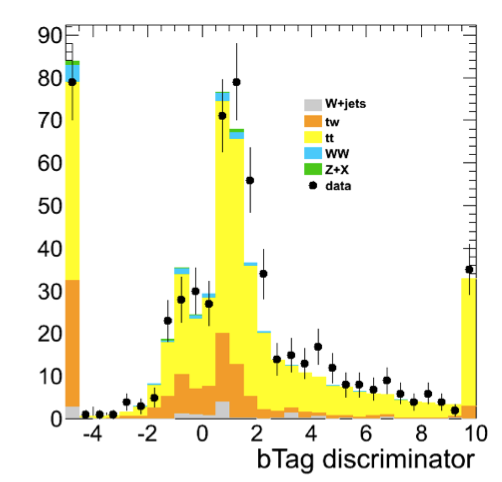
\includegraphics[width=0.3\linewidth]{figures/jetLowBtag_denum_dr.png} 
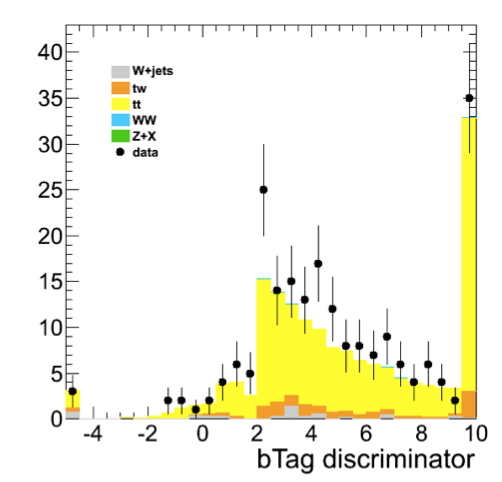
\includegraphics[width=0.3\linewidth]{figures/jetLowBtag_num_dr.png}
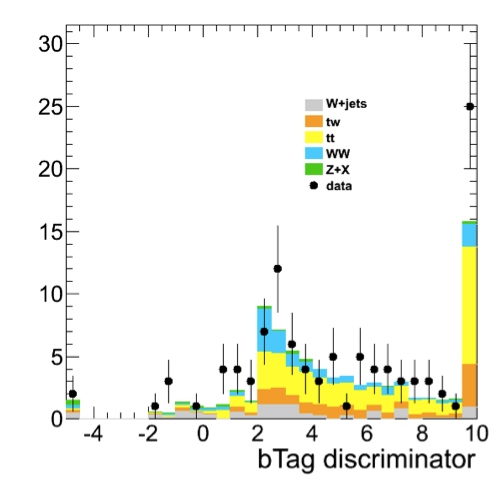
\includegraphics[width=0.3\linewidth]{figures/jetLowBtag_topTag_dr.png}
\caption{\label{fig:jetLowBtag}\protect b-tag discrimiator distribution for 
the jet with $p_T<30$ GeV and the highest b-tag discriminator in the
1-Jet (denumerator, left and numerator, center) and 0-Jet bins control
region (right).}
\end{center}
\end{figure}

   \subsection{$\dyee$ and $\dymm$ Backgrounds}
     \label{sec:bkg_dy}
     Since the production cross-section for Drell-Yan is several orders of magnitude 
higher than the $H \to ZZ$ signal, the Drell-Yan background poses a significant 
challenge. To the leading order, the Drell-Yan process does not contain \met\,  
and therefore its contribution is signficantly reduced by a tight \met selection. 
The residual Drell-Yan contribution in the signal region 
is mainly due to events with fake \met either due to energy mismeasurement of  
the hadronic recoil or momentum mismeasurement of the selected leptons. 
The contribution of events with fake \met due to the lepton momentum mismeasurement 
is expected to be small since we select events within a fairly tight (within $15$ GeV) window 
around the $Z$ boson pole mass. The background due to mismeasurement of the hadronic
recoil is the main source of Drell-Yan events contributing to the selected signal region.

The estimation of residual Drell-Yan background in the signal region depends highly 
our understanding of the \met tails which is sensitive to many factors such as 
the jet energy corrections, the number of pileup interactions, and energy from out of time
contributions. These effects are difficult to model precisely in the simulation.
Therfore we employ a data-driven method to estimate the \met distribution for the 
Drell-Yan background. For events without natural \met\, under the assumption that 
the fake \met is only resulting from mismeasurement of the hadronic recoil, we can use
$\gamma$+jets events as a control sample to predict the \met distribution in $Z$+jets
background events. If parameterized correctly in an observable that is highly correlated 
with the source of fake \met, one expects $\gamma$+jets events to provide an accurate
model of the \met distribution for $Z$+jets events, provided that the photon
is well measured and does not contribute to the \met.

\subsubsection{Photon Selection and Reweighting Procedure}
The photon data sample is selected by requiring one and only one photon passing reaonsably tight
identification and isolation requirements, summarized in Table \ref{tab:PhotonSelection} below 
\cite{MITHggNote}. 
An electron veto is imposed on the photon, requiring that no GSF electron which does not match to 
one leg of a well reconstructed convert is sharing the same supercluster as the photon
candidate. This is intended to reduce contributions from W bosons decaying to electrons, misidentified
as photons. To reduce contamination from $W$+$\gamma$ events, we veto any events with one or 
more well identified leptons.


\begin{table}[!ht]
\begin{center}
\begin{tabular}{|c|c|} 
\hline
Cut           & Requirement                                                                           \\
\hline
$\eta$        & $|\eta| < 1.4442$                                                                     \\ 
\hline
H/E           & H/E $< 0.05$                                                                          \\
\hline
Electron Veto & Photon is rejected if it shares the supercluster with an electron that does not       \\
              & match to one leg of a conversion with $\mathrm{L}_{\mathrm{xy}} < 2.0$, fit           \\
              & probability  $> 10^{-6}$, and no hits behind the fitted vertex                        \\
\hline
\hline
\multicolumn{2}{|c|}{Conversion ID (if matched to a conversion with $\mathrm{L}_{\mathrm{xy}} < 2.0$,}\\
\multicolumn{2}{|c|}{fit probability $> 10^{-6}$, and at most one hit before the fitted vertex on }   \\
\multicolumn{2}{|c|}{either of the tracks forming the conversion) }                                   \\
\hline
E/P            & E/P $< 2.0 $                                                                         \\
%$\Delta\eta$  & $|\Delta\eta| < 0.01 for Endcap only$ \\
%$\Delta\phi$  & $|\Delta\phi| < 0.01 for Endcap only$ \\
\hline
\hline
\multicolumn{2}{|c|}{Isolation}                                                                       \\
\hline
EcalIso       & EcalIso $ - \rho\times \mathrm{A}_{\mathrm{eff Ecal}}$ $<  2.0 + 0.006\times p_{T}$   \\
HcalIso       & HcalIso $ - \rho\times \mathrm{A}_{\mathrm{eff Hcal}}$ $<  2.0 + 0.0025\times p_{T}$  \\
TrkIso        & TrkIso $ - \rho\times \mathrm{A}_{\mathrm{eff Trk}}$ $<  1.5 + 0.001\times p_{T}$     \\
\hline

%\hline
%SpikeKilling & \\
%\hline
%$E_{\mathrm{Max}} / E_{9}$ & $E_{\mathrm{Max}} / E_{9} > 0.95$       \\
%$\sigma_{i\eta i\eta}$     & $\sigma_{i\eta i\eta} > 0.001$          \\
%$\sigma_{i\phi i\phi}$     & $\sigma_{i\phi i\phi} > 0.001$          \\
%\hline

\hline
\end{tabular}
\caption{MC yield prediction for $H\rightarrow WW$ sample ($m_H=130$ GeV) ($\mu$-e and e-e final states). 
The electron selection is the same as in 2010 analysis and the results is scaled to 1/fb.
\label{tab:PhotonSelection}}
\end{center}
\end{table}


Since the fake \met is due to mismeasurement of the hadronic recoil, we parameterize the 
modelling of the \met distribution in the $p_{T}$ of the photon / dilepton system and 
the number of counted jets. Both variables are highly correlated with the behavior 
of the hadronic recoil. Reweighting factors are computed in bins of the number of counted jets
and the dilepton $p_{T}$ by dividing the corresponding two dimensional distributions
in the $\gamma$+jets data sample and the dilepton data sample:

\begin{eqnarray}
  w(p_{T},\mathrm{njet}) = \frac{\mathrm{N}_{\gamma+\mathrm{jets}}(p_{T},\mathrm{njet})}{\mathrm{N}_{\mathrm{Z+jets}}(p_{T},\mathrm{njet})}.
\end{eqnarray}

In order for these reweighting factors to be insensitive to the presence of signal or backgrounds with 
real \met, we build these weight factors on a $\gamma$+jets and $Z$+jets sample imposing an anti-selection
on the \met : $\met < 30$ GeV. For the $Z$+jets sample, the full $H \to ZZ$ preselection is imposed, 
including the top veto and the third lepton veto.

Finally, to model the \met distribution for the final selection we select $\gamma$+jets events
as above, imposing the preselection requirement that the photon $p_{T}$ is greater than $40$GeV,
and associate the corresponding weight factor $w(p_{T},\mathrm{njet})$ to each such event. To build
the track \met in the $\gamma$+jets events, we must consistently account for the momentum of
the photon since we intend it to model the dilepton system which would be included in the 
track \met in $Z$+jets events. To mitigate cases of inconsistencies between the particle flow 
photon reconstruction and the standard photon reconstruction, particularly for converted photons,
we do not include any charged particle flow candidates inside the ($\Delta$R $<0.4$) isolation cone 
of the photon in the track \met sum.
To model the transverse mass distribution, we draw a random number from a pre-determined dilepton
mass distribution and build the $m_{T}$ observable as in Eqn \ref{}. The dilepton mass distribution
is constructed from data imposing all preselection cuts except the \met requirement.

\subsubsection{Monte Carlo Closure Test}

In order to verify that the procedure models the $Z$+jet background well, we test it
in $\gamma$+jets and $Z$+jets Monte Carlo simulation. The reweighting factors are 
built from the simulation sample according to the procedure described above and then 
applied on the $\gamma$+jets Monte Carlo sample. 

%The photon and $Z$ 
%$p_{T}$ distributions are shown in Fig \ref{fig:PhotonJetsClosureTest_Pt} to demonstrate that 
%the reweighting is carried out consistently.

%% \begin{figure}[!htbp]
%% \begin{center}
%% \subfigure[0-Jet]{\includegraphics[width=0.45\textwidth]{figures/PhotonJetsClosureTest_0Jet_Pt.pdf}}
%% \subfigure[1-Jet]{\includegraphics[width=0.45\textwidth]{figures/PhotonJetsClosureTest_1Jet_Pt.pdf}}
%% \subfigure[2-Jet]{\includegraphics[width=0.45\textwidth]{figures/PhotonJetsClosureTest_2Jet_Pt.pdf}}
%% \caption{Comparison of the dilepton $p_{T}$ and the photon $p_{T}$ before and after reweighting.}
%% \label{fig:PhotonJetsClosureTest_Pt}
%% \end{center}
%% \end{figure}


In Fig \ref{fig:PhotonJetsClosureTest_TrackMET} we show the particle flow \met distribution 
from the $\gamma$+jet sample after reweighting compared to the \met distribution from the 
$Z$+jet sample, separately in the 0-jet, 1-jet, and 2-jet bins. We observe agreement between 
the $\gamma$+jet generated prediction and the $Z$+jet simulation particle flow \met distribution. 
In Fig \ref{fig:PhotonJetsClosureTest_TrackMET} we show the analogous comparison for track \met, where 
is agreement slightly worse than for particle flow \met. Finally, in 
Fig \ref{fig:PhotonJetsClosureTest_TrackMET}, we show the comparison for the minimum of the 
track \met and the particle flow \met, which shows better agreement than the track \met alone. 

\begin{figure}[!htbp]
\begin{center}
\subfigure[0-Jet]{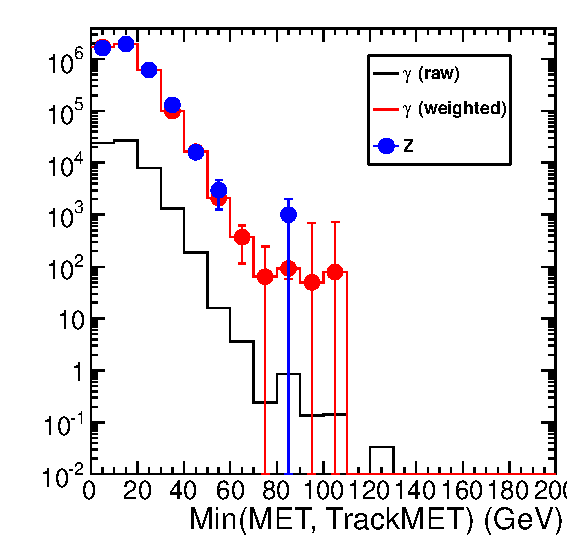
\includegraphics[width=0.45\textwidth]{figures/PhotonJetsClosureTest_0Jet_PFMET.pdf}}
\subfigure[1-Jet]{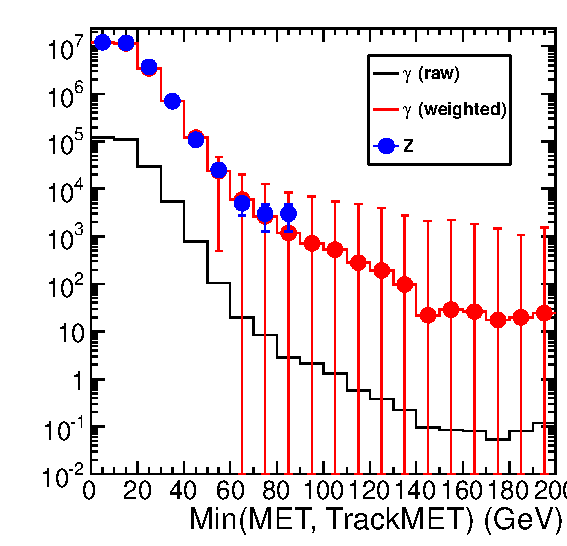
\includegraphics[width=0.45\textwidth]{figures/PhotonJetsClosureTest_1Jet_PFMET.pdf}}
\subfigure[2-Jet]{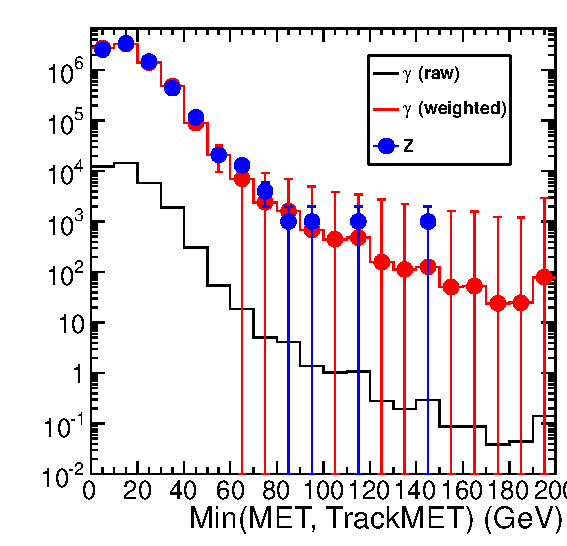
\includegraphics[width=0.45\textwidth]{figures/PhotonJetsClosureTest_2Jet_PFMET.pdf}}
\caption{Comparison of the particle flow \met prediction from the reweighted $\gamma$+jets sample
and the simulation prediction from the $Z$+jets sample.}
\label{fig:PhotonJetsClosureTest_TrackMET}
\end{center}
\end{figure}

\begin{figure}[!htbp]
\begin{center}
\subfigure[0-Jet]{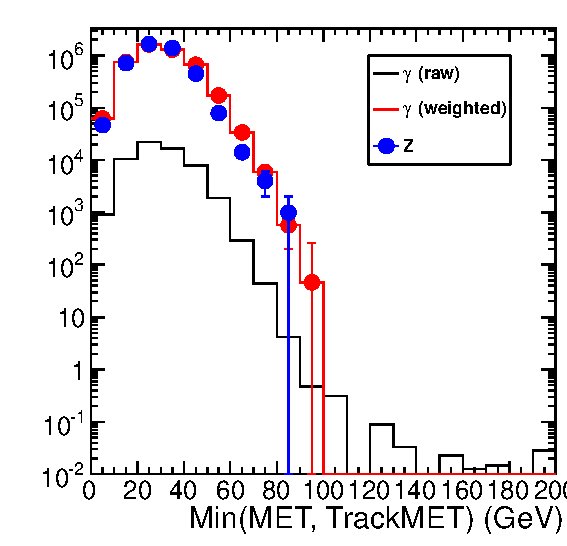
\includegraphics[width=0.45\textwidth]{figures/PhotonJetsClosureTest_0Jet_TrackMET.pdf}}
\subfigure[1-Jet]{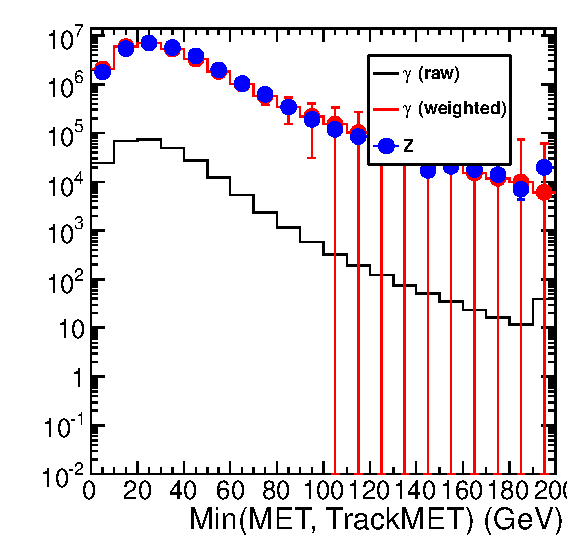
\includegraphics[width=0.45\textwidth]{figures/PhotonJetsClosureTest_1Jet_TrackMET.pdf}}
\subfigure[2-Jet]{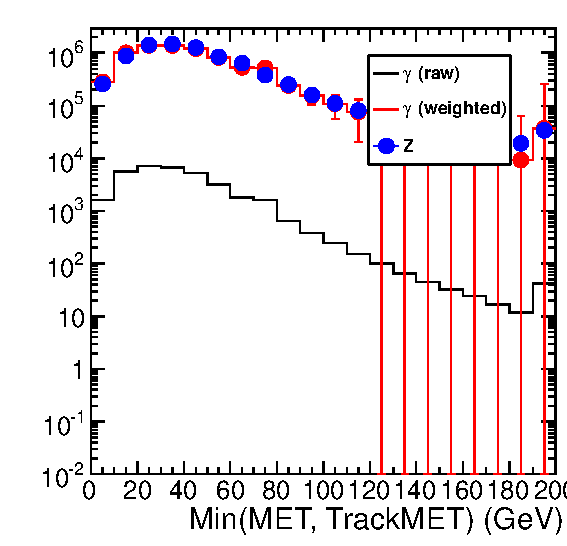
\includegraphics[width=0.45\textwidth]{figures/PhotonJetsClosureTest_2Jet_TrackMET.pdf}}
\caption{Comparison of the particle flow track \met prediction from the reweighted $\gamma$+jets sample
and the simulation prediction from the $Z$+jets sample.}
\label{fig:PhotonJetsClosureTest_TrackMET}
\end{center}
\end{figure}

\begin{figure}[!htbp]
\begin{center}
\subfigure[0-Jet]{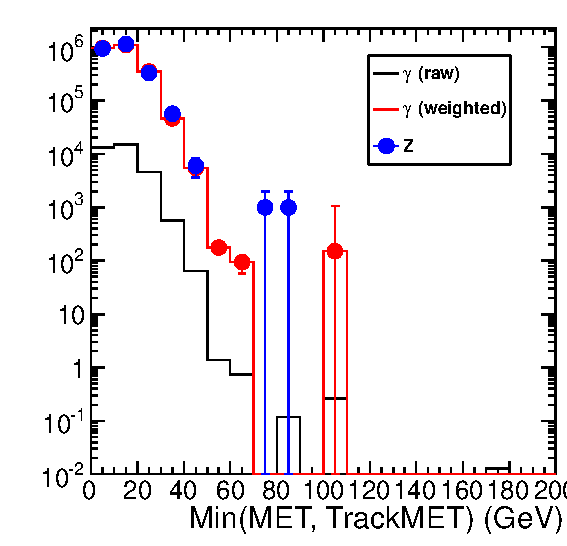
\includegraphics[width=0.45\textwidth]{figures/PhotonJetsClosureTest_0Jet_MinMET.pdf}}
\subfigure[1-Jet]{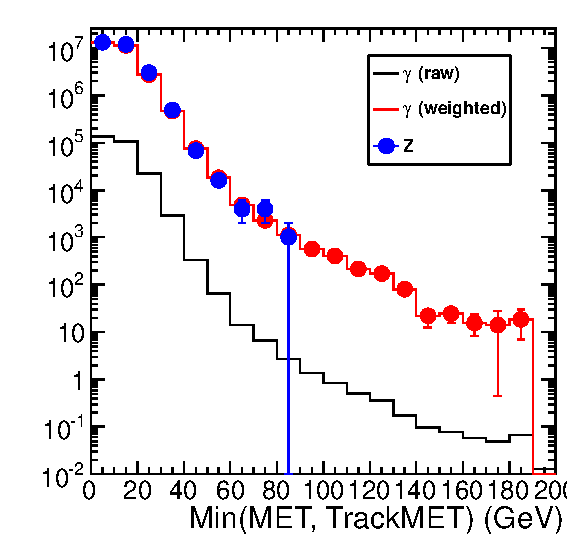
\includegraphics[width=0.45\textwidth]{figures/PhotonJetsClosureTest_1Jet_MinMET.pdf}}
\subfigure[2-Jet]{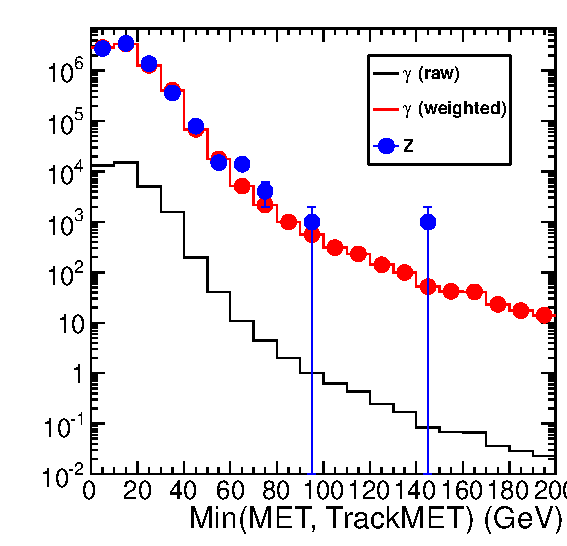
\includegraphics[width=0.45\textwidth]{figures/PhotonJetsClosureTest_2Jet_MinMET.pdf}}
\caption{Comparison of the minimum of particle flow \met and particle flow track \met prediction from
the reweighted $\gamma$+jets sample and the simulation prediction from the $Z$+jets sample.}
\label{fig:PhotonJetsClosureTest_TrackMET}
\end{center}
\end{figure}

\begin{figure}[!htbp]
\begin{center}
\subfigure[0-Jet]{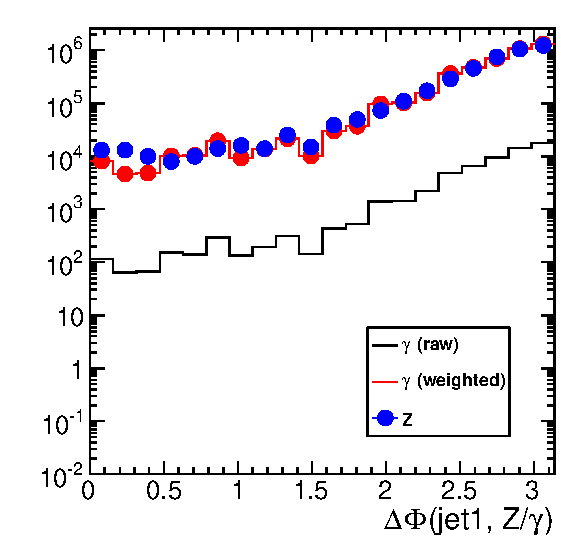
\includegraphics[width=0.45\textwidth]{figures/PhotonJetsClosureTest_0Jet_Dphi.pdf}}
\subfigure[1-Jet]{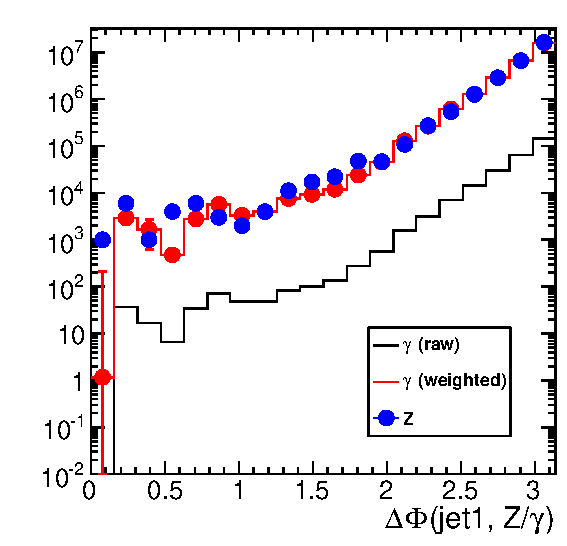
\includegraphics[width=0.45\textwidth]{figures/PhotonJetsClosureTest_1Jet_Dphi.pdf}}
\subfigure[2-Jet]{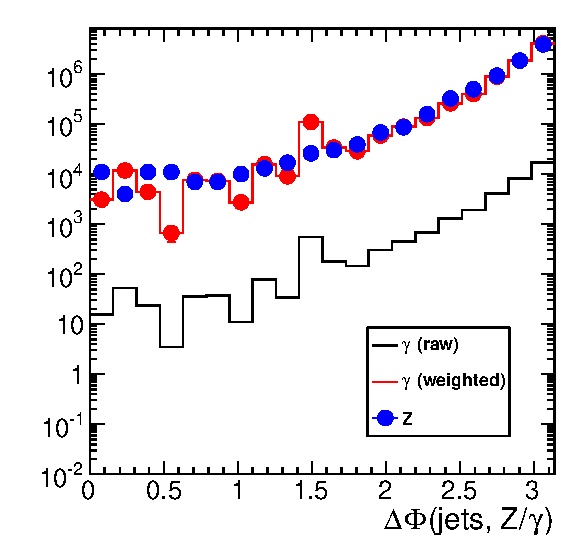
\includegraphics[width=0.45\textwidth]{figures/PhotonJetsClosureTest_2Jet_Dphi.pdf}}
\caption{Comparison of the $\Delta\phi$ between the dilepton system and the leading jet 
(with $p_{T} > 15$ GeV) in the event between the reweighted $\gamma$+jets sample and the 
simulation prediction from the $Z$+jets sample.}
\label{fig:PhotonJetsClosureTest_DPhi}
\end{center}
\end{figure}


Finally, we show the comparison between the predicted transverse mass distribution and the simulation
distribution with no cut on minimum \met in Fig \ref{fig:PhotonJetsClosureTest_MtHZZ_NoMetCut} and 
with a minimum \met cut of greater than $40$GeV in Fig \ref{fig:PhotonJetsClosureTest_MtHZZ_MetPresel}. 
The predicted shape and the simulation shape are again in reasonable agreement. 

\begin{figure}[!htbp]
\begin{center}
\subfigure[0-Jet]{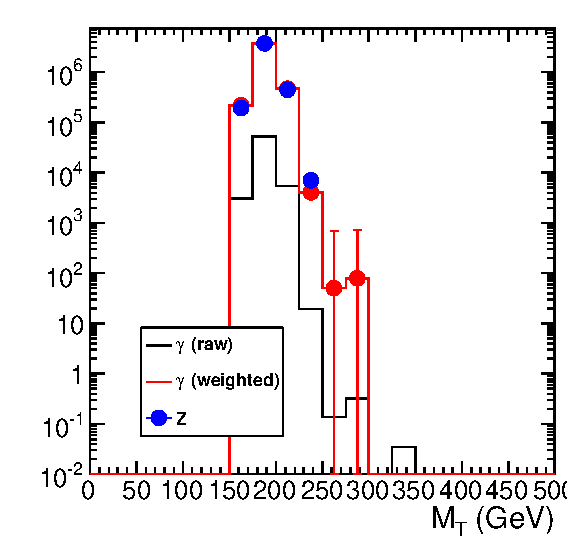
\includegraphics[width=0.45\textwidth]{figures/PhotonJetsClosureTest_0Jet_MtHZZ_NoMetCut.pdf}}
\subfigure[1-Jet]{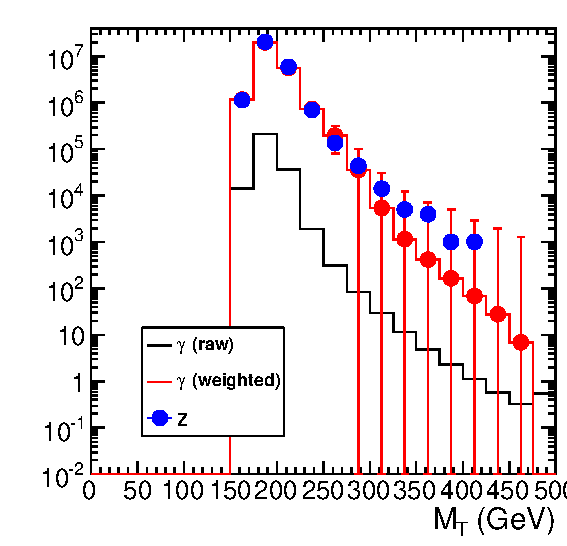
\includegraphics[width=0.45\textwidth]{figures/PhotonJetsClosureTest_1Jet_MtHZZ_NoMetCut.pdf}}
\subfigure[2-Jet]{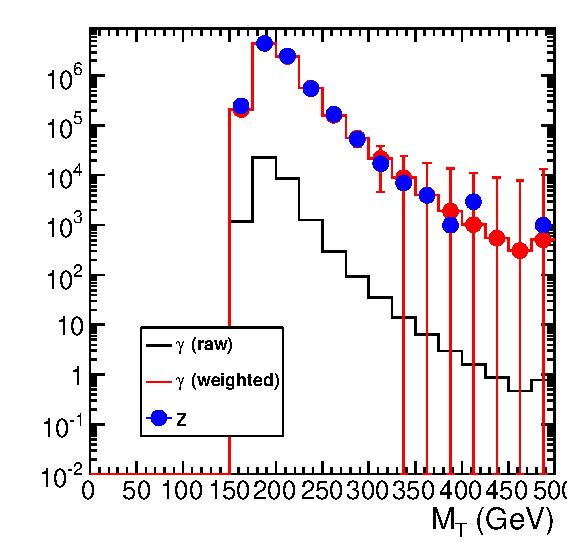
\includegraphics[width=0.45\textwidth]{figures/PhotonJetsClosureTest_2Jet_MtHZZ_NoMetCut.pdf}}
\caption{Comparison of the transverse mass prediction from the reweighted $\gamma$+jets sample 
and the simulation prediction from the $Z$+jets sample, where no \met cut has been applied.}
\label{fig:PhotonJetsClosureTest_MtHZZ_NoMetCut}
\end{center}
\end{figure}

\begin{figure}[!htbp]
\begin{center}
\subfigure[0-Jet]{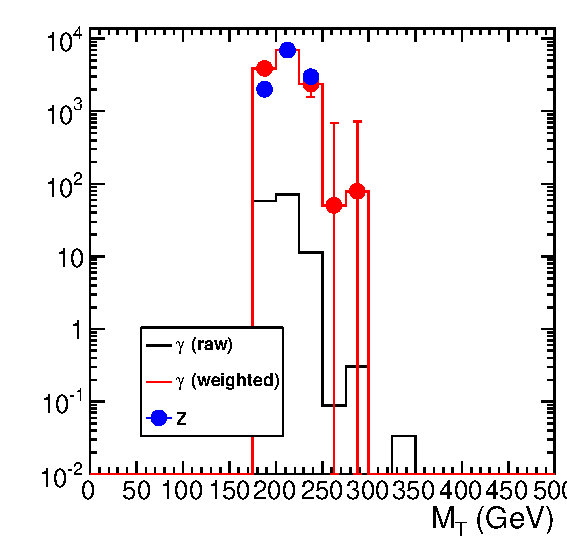
\includegraphics[width=0.45\textwidth]{figures/PhotonJetsClosureTest_0Jet_MtHZZ_MetPresel.pdf}}
\subfigure[1-Jet]{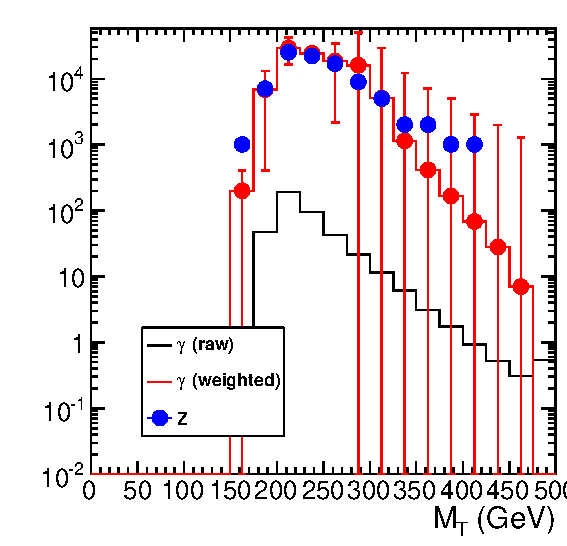
\includegraphics[width=0.45\textwidth]{figures/PhotonJetsClosureTest_1Jet_MtHZZ_MetPresel.pdf}}
\subfigure[2-Jet]{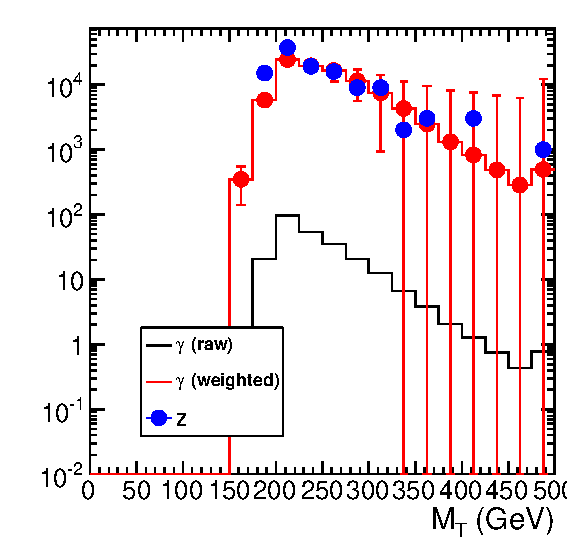
\includegraphics[width=0.45\textwidth]{figures/PhotonJetsClosureTest_2Jet_MtHZZ_MetPresel.pdf}}
\caption{Comparison of the transverse mass prediction from the reweighted $\gamma$+jets sample 
and the simulation prediction from the $Z$+jets sample, where the minimum \met is required to be larger than 
$40$ GeV. }
\label{fig:PhotonJetsClosureTest_MtHZZ_MetPresel}
\end{center}
\end{figure}


%We work on this section more later
%\subsubsection{Systematic Uncertainties}

Based on the degree of overall disagreement in the full range of the minimum \met we assign 
systematic uncertainties of $30\%$ in all the jet bins.


\subsubsection{Data Estimate}

The predictions for the minimum \met is compared with the results obtained in the first $187$\ipb 
of Run2011 data in Fig \ref{}, separately for the 0-jet, 1-jet, and 2-jet bins. Including all of the
backgrounds with real \met, we obtain reasonable agreement with data. 

Based on the $\gamma$+jet sample prediction, we obtain the background predictions for the
preselection and all the mass dependent cut-based analyses summarized in Table \ref{tab:DYBkgPrediction}.

\begin{table}[!htbp]
\begin{center}
\begin{tabular}{|l|c|c|c|c|}
\hline
Higgs Mass      &  0-jet bin             & 1-jet bin             & 2-jet bin             & Total                \\
\hline
ZZ Preselection &  $0.01 \pm 0.00$(stat) & $0.08 \pm 0.02$(stat) & $0.22 \pm 0.07$(stat) $ 0.31 \pm 0.11$(stat) \\
\hline
250             &  $0.01 \pm 0.00$(stat) & $0.08 \pm 0.02$(stat) & $0.22 \pm 0.07$(stat) $ 0.31 \pm 0.11$(stat) \\
300             &  $0.01 \pm 0.00$(stat) & $0.08 \pm 0.02$(stat) & $0.22 \pm 0.07$(stat) $ 0.31 \pm 0.11$(stat) \\
400             &  $0.01 \pm 0.00$(stat) & $0.08 \pm 0.02$(stat) & $0.22 \pm 0.07$(stat) $ 0.31 \pm 0.11$(stat) \\
\hline
\end{tabular}
\caption{Summary of $Z$+jets background yields estimated using $\gamma$+jets events in 187 $\ipb$.}
\label{tab:DYBkgPrediction}
\end{center}
\end{table}
%   \subsection{$\dytt$ Background}
%     \label{sec:bkg_dytt}
%     In previous studies of the \WW\ final state the \dytt\ contribution
was considered small and well reproduced by the simulation since this
final state has a natural source of \met\ - neutrinos from $\tau$
decays. The fact that \met\ tends to be alligned with one of the
leptons is explored in the projected \met\ variable definition to
reduce the background rate.

With a rapid increase in the number of multiple interactions per bunch
crossing in 2011 data the situation is changing. Large amount of
pileup may lead to fake \met\ that is larger than the natural \met\
in \dytt\ events. Given that the \dytt\ cross-section is large and the
fact that we use a lower \met\ threshold in \emu\ final state we need
to make sure that this background is under control and reliably
estimated. Since the simulations that we have at the moment do not
reproduce the fake \met\ observed in data, we need a data-driven
method for the \dytt\ background estimation.

In order to estimate the \dytt\ background from data we can use \zee\
and \zmm\ events replacing electrons and muons with a simulated
$\tau\to l\nu_\tau\bar{\nu_e}$ decay - final state leptons will
represent the dilepton pair and neutrinos will modify obseved \met{}.

Neglecting masses of electron, muon and neutrinos the angular
distribution of electron or muon originating from $\tau$ decay in
$\tau$ rest frame is:
\begin{equation}
        \frac{d^2\Gamma}{dx\,d\cos\theta}\sim x^2(3-2x \pm P\cos\theta(2x-1))
\end{equation}
where $\theta$ is the helicity angle, i.e. angle between $\tau$ and
lepton direction in $\tau$ rest frame, $x=2E_l/m_\tau$ - reduced
energy, i.e. the energy of the lepton over its maximum allowed energy
and $P$ is degree of $\tau$ polarization~\cite{pdg}.

Figure~\ref{fig:dytt_closure} shows a comparison of some kinematic
distributions of \dytt\ Monte Carlo and a prediction based on \dymm\
Monte Carlo events using the procedure described above.

%% %%%%%%%%%%%%%%%%%%%%%%%%%%%%%%
%% \begin{figure}[!htbp]
%% \begin{center}
%% 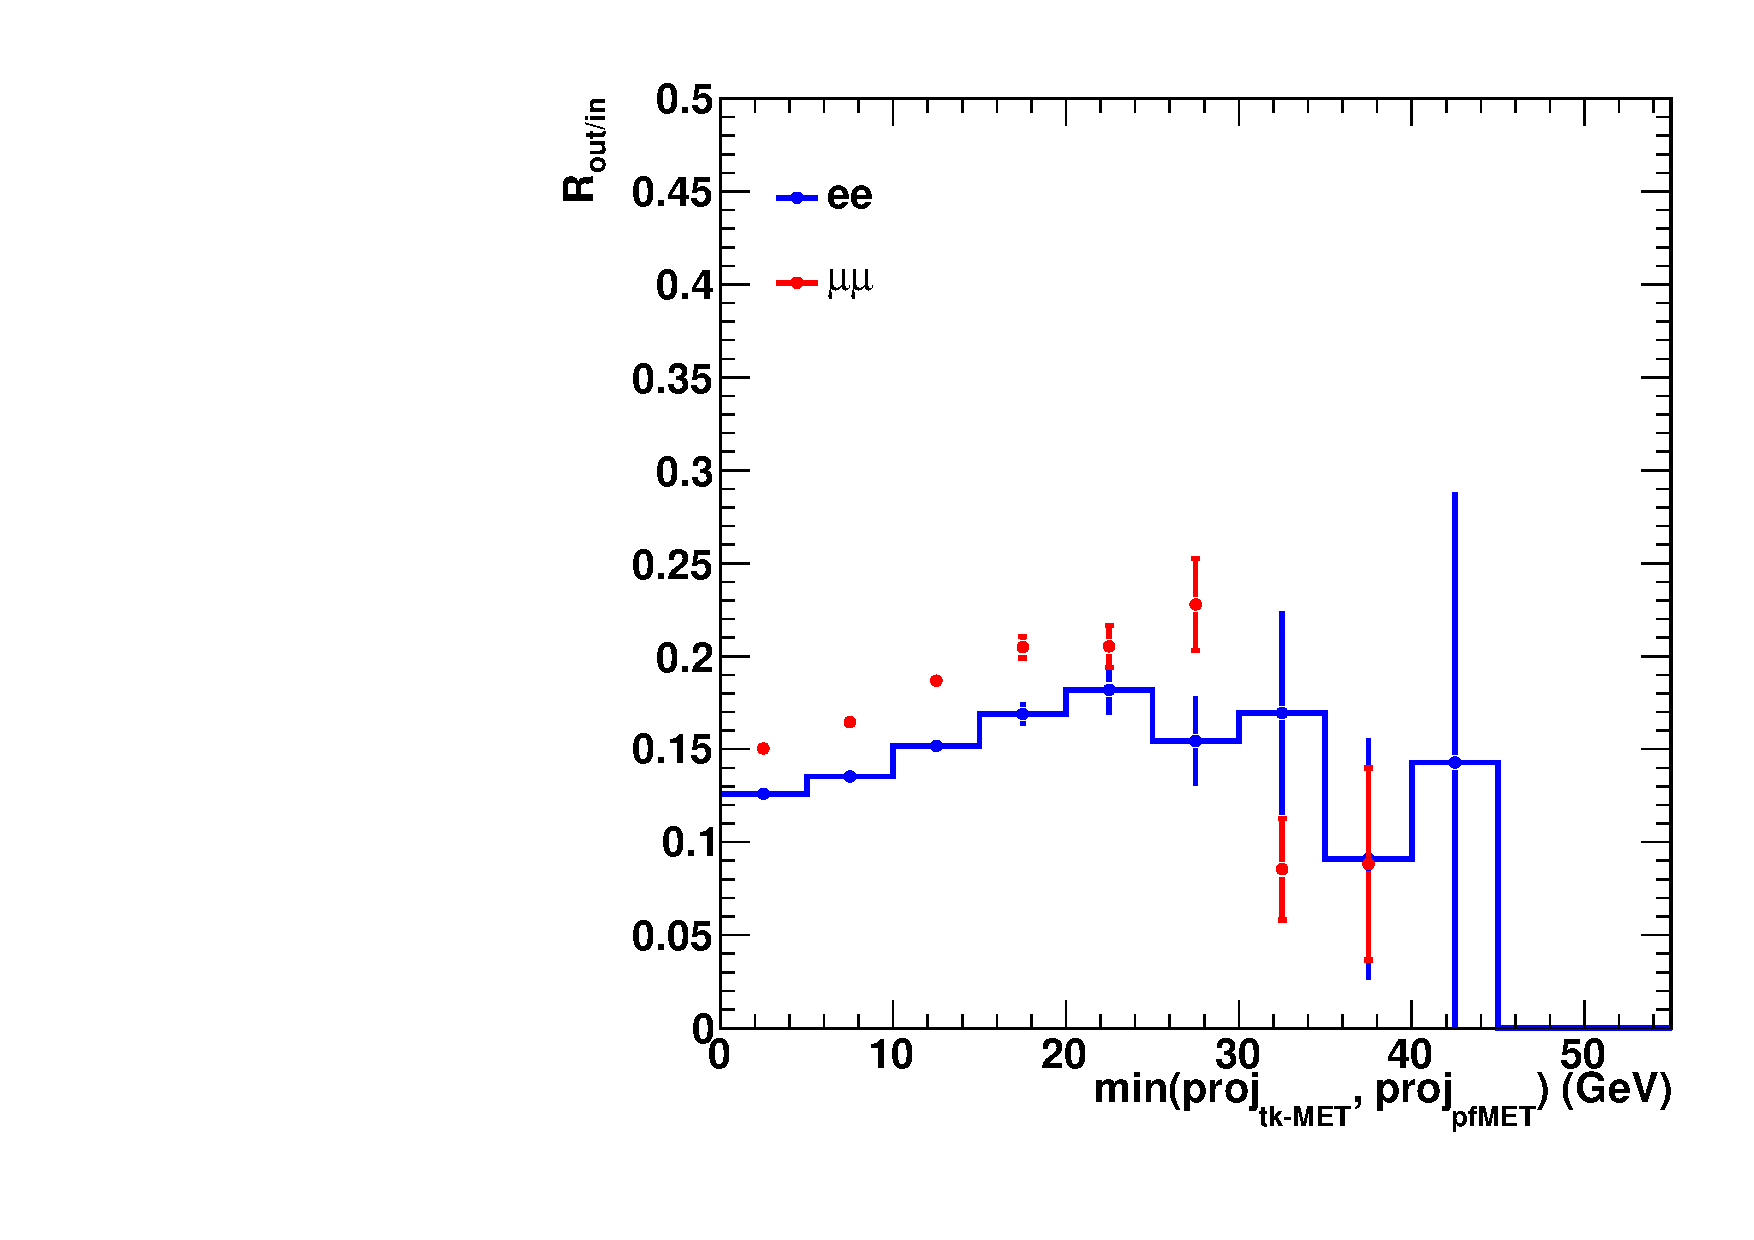
\includegraphics[width=0.3\textwidth]{figures/Routin_mc_0Jet.pdf}
%% 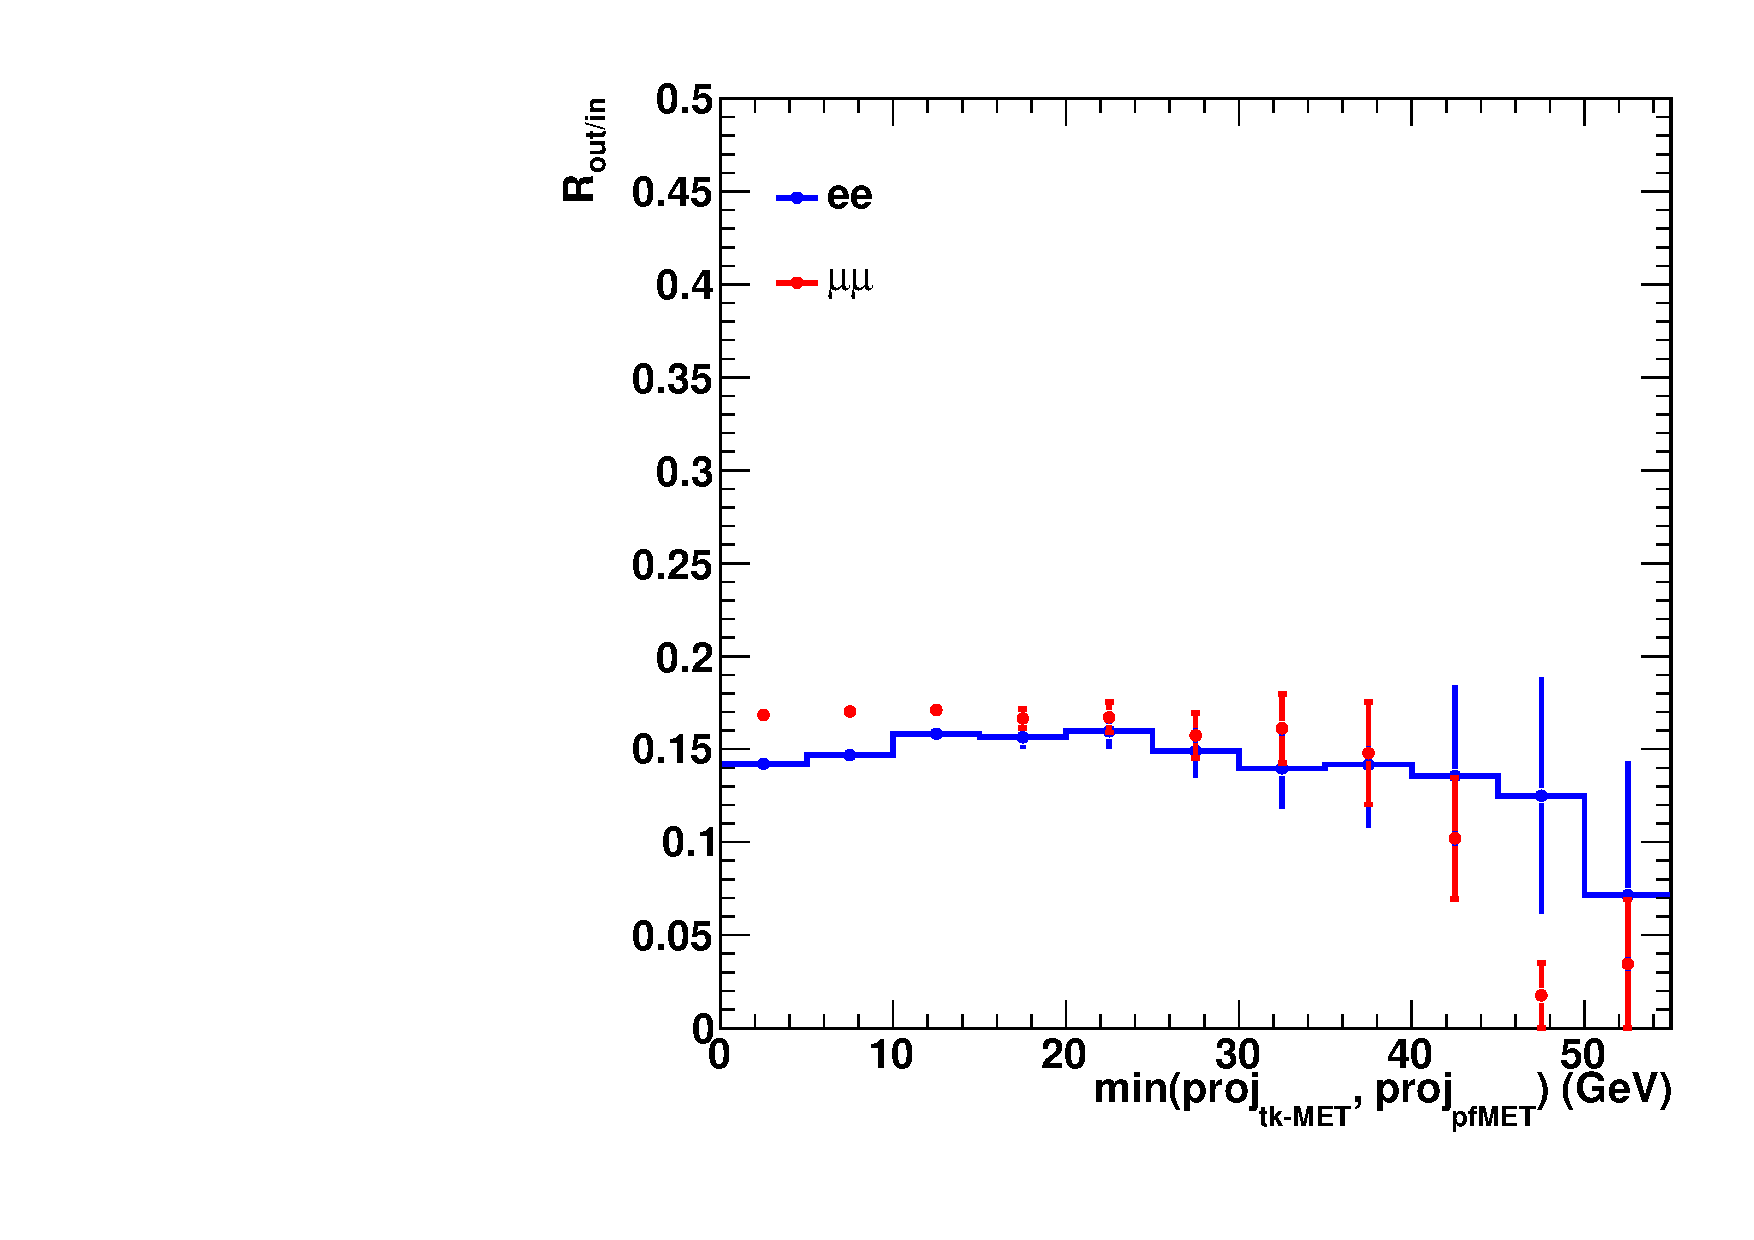
\includegraphics[width=0.3\textwidth]{figures/Routin_mc_1Jet.pdf}
%% 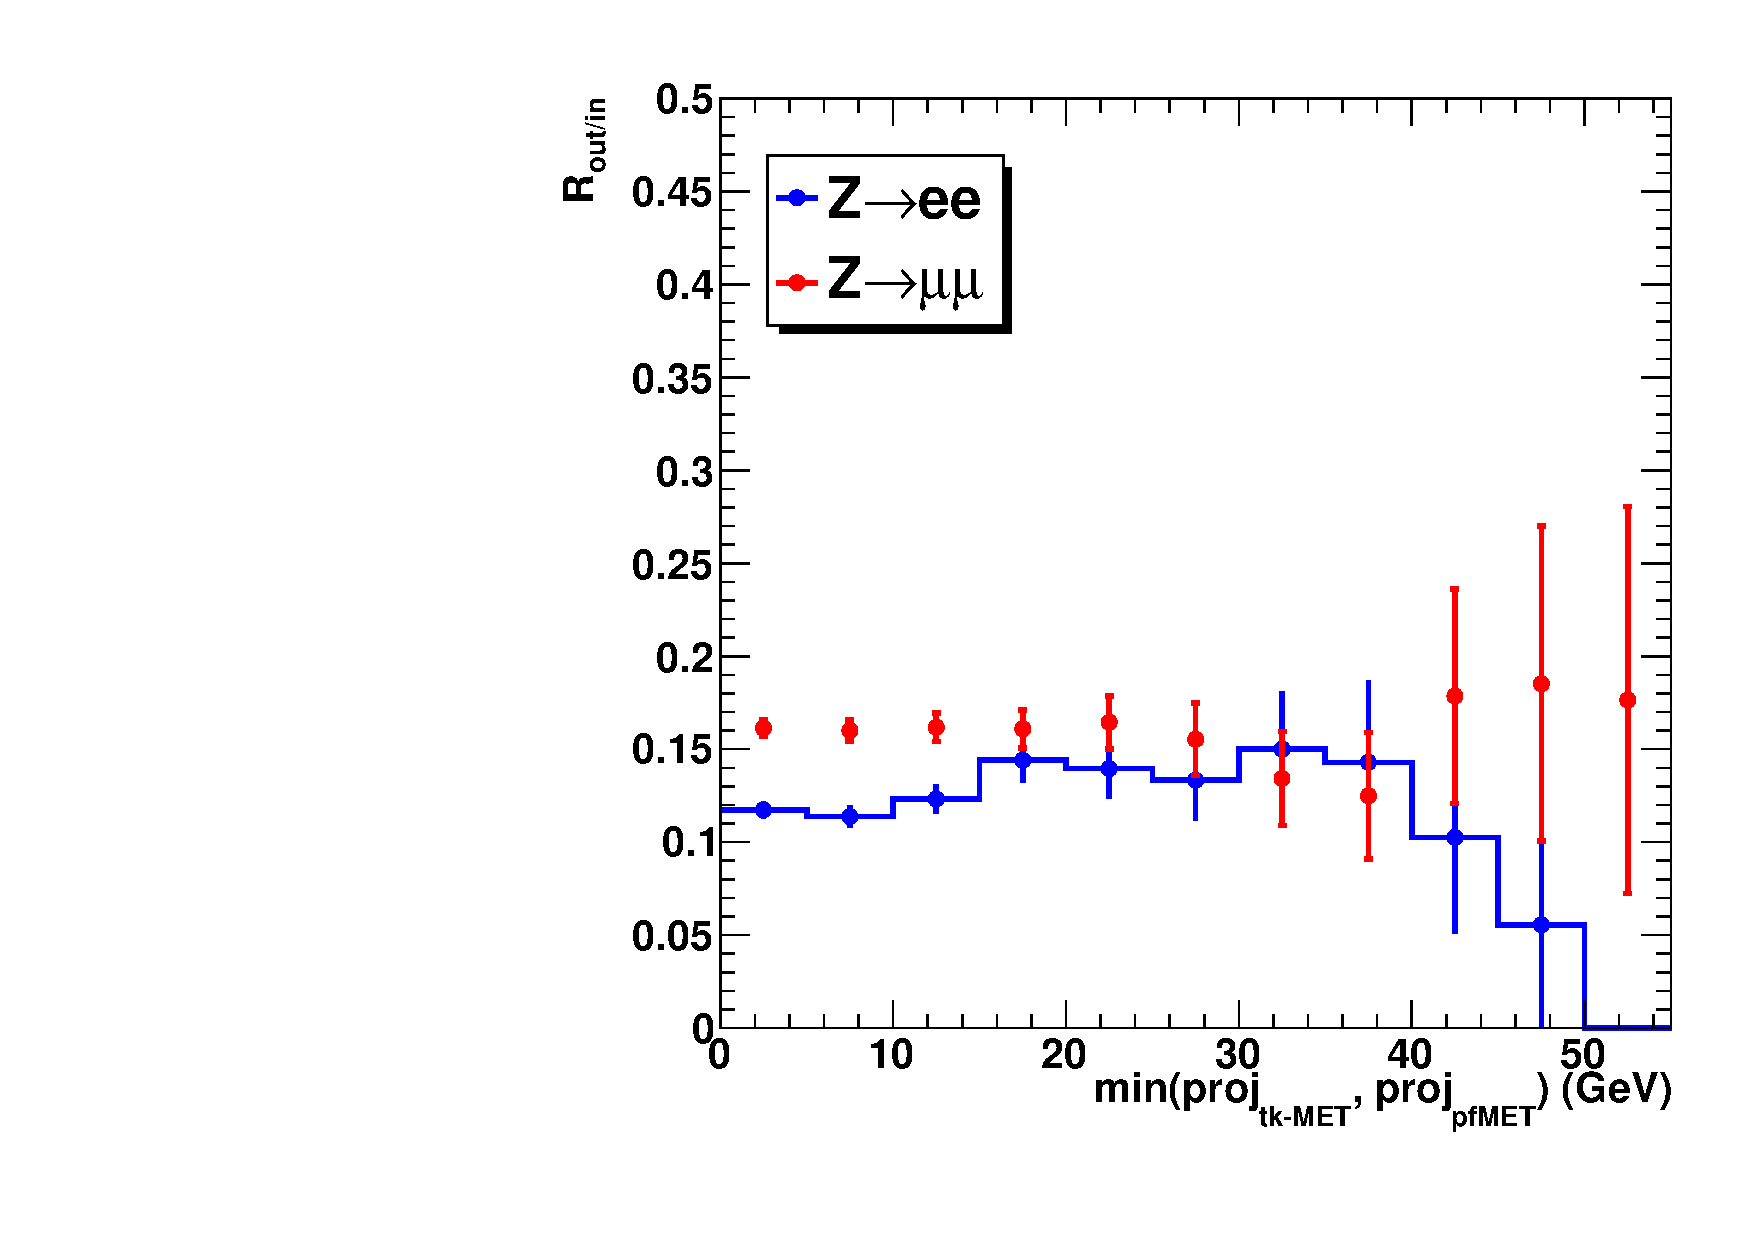
\includegraphics[width=0.3\textwidth]{figures/Routin_mc_2Jet.pdf}
%% \caption{ The ratio $R_{out/in}$ as a function of the $\met$ cut obtained using MC in the 
%% 0-Jet (left), 1-Jet (middle) and 2-Jet (right) bins. The event content in each 
%% bin is uncorrelated. The last bin represent the $R_{out/in}$ measured with min-MET $>$ 40 GeV. 
%% } %The difference in the ratio between 
%% %\ee\ and \mm\ final states is due to lower minimum muon momentum compared with electron
%% %(10 GeV vs 15 GeV), which allows for more low mass Drell-Yan events.}
%% \label{fig:routin_met}
%% \end{center}
%% \end{figure}
%% %%%%%%%%%%%%%%%%%%%%%%%%%%%%%%


%% We apply a data-driven method~\cite{dyestnote} to estimate the $\dyll$
%% contributions in the same flavor $\ell^+\ell^-$ final states. %This
%% %method also provides an estimate for the \emph{resonant component} of
%% %$WZ$ and $ZZ$ contributions, in which both leptons come from the same
%% %$Z$ boson.

%% The expected contributions from $\dyll$ events outside the $Z$-mass
%% region in data can be estimated by counting the number of events near
%% the $Z$ mass region in data, subtracting from it the non-$Z$
%% contributions, and scaling it by a ratio $R_{out/in}$ defined as the
%% fraction of events outside and inside the $Z$-mass region in the
%% simulation. The non-$Z$ contributions close to the $Z$-mass region in
%% data is estimated from the number of events in the $e^\pm\mu^\mp$
%% final state $N_{in}^{e\mu}$, applying a correction factor that
%% normalizes the electron-to-muon efficiency $k_{ee/\mu\mu}$. 
%% $R_{out/in}$ can be obtained both from simulation and
%% data.  In simulation it is defined as the ratio
%% $N_{out}^{MC}/N_{in}^{MC}$. 
%% %$N_{out}^{MC}/N_{in}^{MC}$ with a looser $\met$ cut of 20 GeV
%% %(referred to as a loose selection).  This method is described
%% This method is described mathematically in Eq.~\ref{eq:dyest}.
%% %%%%%%%%%%%%%%%%%%%%%%%%%%%%%%
%% \begin{eqnarray}
%% %N_{out}^{ll,exp} = R_{out/in}^{ll,loose}(N_{in}^{ll} - 0.5N_{in}^{e\mu}k_{ll}), 
%% N_{out}^{ll,exp} = R_{out/in}^{ll}(N_{in}^{ll} - 0.5N_{in}^{e\mu}k_{ll}), 
%% \label{eq:dyest}
%% \end{eqnarray}
%% %%%%%%%%%%%%%%%%%%%%%%%%%%%%%%
%% where $k_{ee} = \sqrt{\frac{N_{in}^{ee,loose}}{N_{in}^{\mu\mu,loose}}}$ for 
%% $\dyee$ and $k_{mm} = \sqrt{\frac{N_{in}^{\mu\mu,loose}}{N_{in}^{ee,loose}}}$ 
%% for $\dymm$. In the $k_{ll}$ calcualtion, we apply a loose $\met$ cut of 20 GeV. 
%% The values of $R_{out/in}$ as estimated from simulation are reported
%% in Table~\ref{tab:Routinmc} at the \ww\ preselection level. 

%% %%%%%%%%%%%%%%%%%%%%%%%%%%%%%%%
%% \begin{table}
%% \begin{center}
%% \begin{tabular}{c c c c }
%% \hline
%% \vspace{-3mm} && \\
%% Jet Bin & $R_{out/in}^{mm}$ &  $R_{out/in}^{ee}$  &   $R_{out/in}^{ee,mm}$\\
%% \vspace{-3mm} &&& \\
%% \hline
%% 0 & 0.23 $\pm$ 0.09 $\pm$ 0.10 & 0.29 $\pm$ 0.09 $\pm$ 0.11 & 0.25 $\pm$ 0.06 $\pm$ 0.05\\
%% 1 & 0.15 $\pm$ 0.04 $\pm$ 0.15 & 0.14 $\pm$ 0.03 $\pm$ 0.05 & 0.15 $\pm$ 0.03 $\pm$ 0.10\\
%% 2 & 0.16 $\pm$ 0.03 $\pm$ 0.13 & 0.13 $\pm$ 0.03 $\pm$ 0.06 & 0.15 $\pm$ 0.02 $\pm$ 0.10\\
%% \hline
%% \end{tabular}
%% \end{center}
%% \caption{The ratio $R_{out/in}^{ll}$ at different jet bins evaluated from MC, applying the min-MET $>$ 40 GeV selection.
%% \label{tab:Routinmc}}
%% \end{table}
%% %%%%%%%%%%%%%%%%%%%%%%%%%%%%%%


%% %%%%%%%%%%%%%%%%%%%%%%%%%%%%%%
%% \begin{figure}[!htbp]
%% \begin{center}
%% 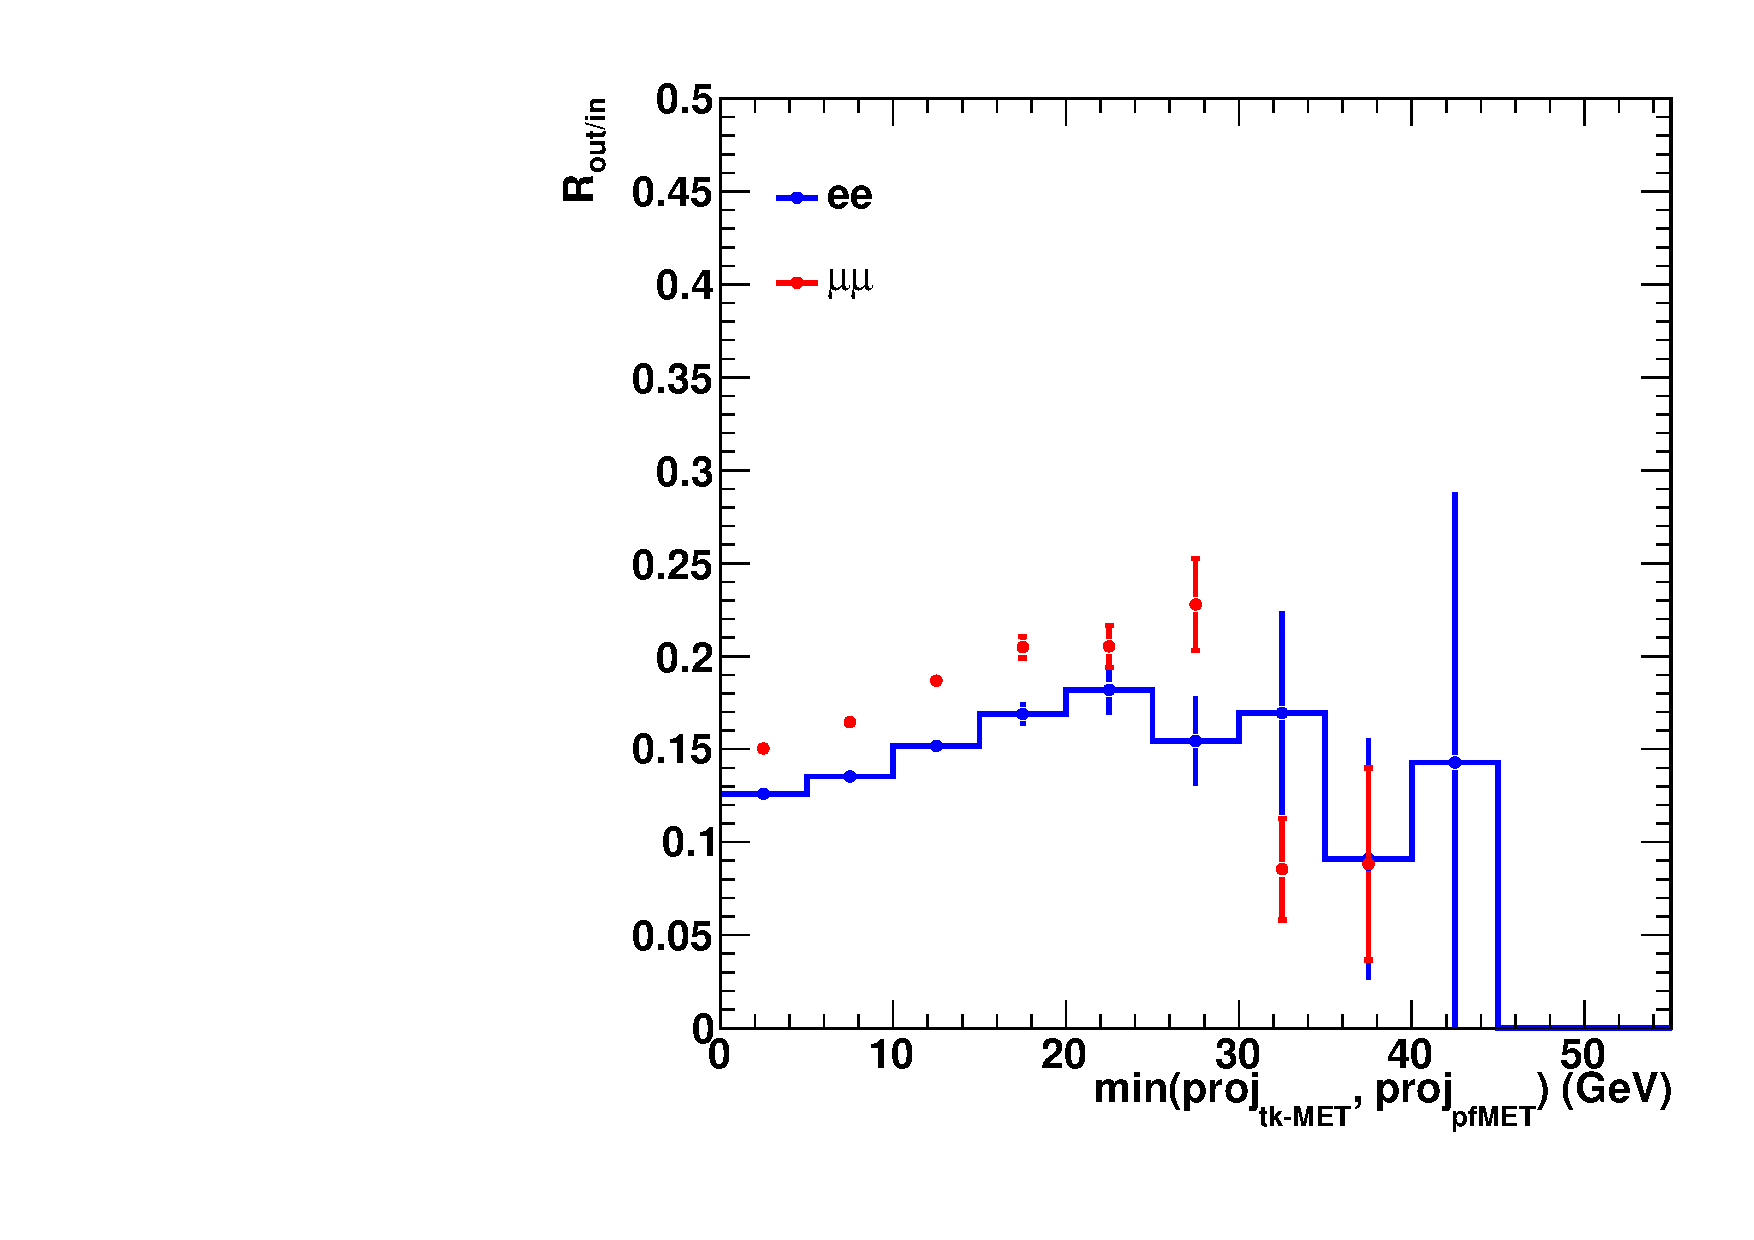
\includegraphics[width=0.3\textwidth]{figures/Routin_mc_0Jet.pdf}
%% 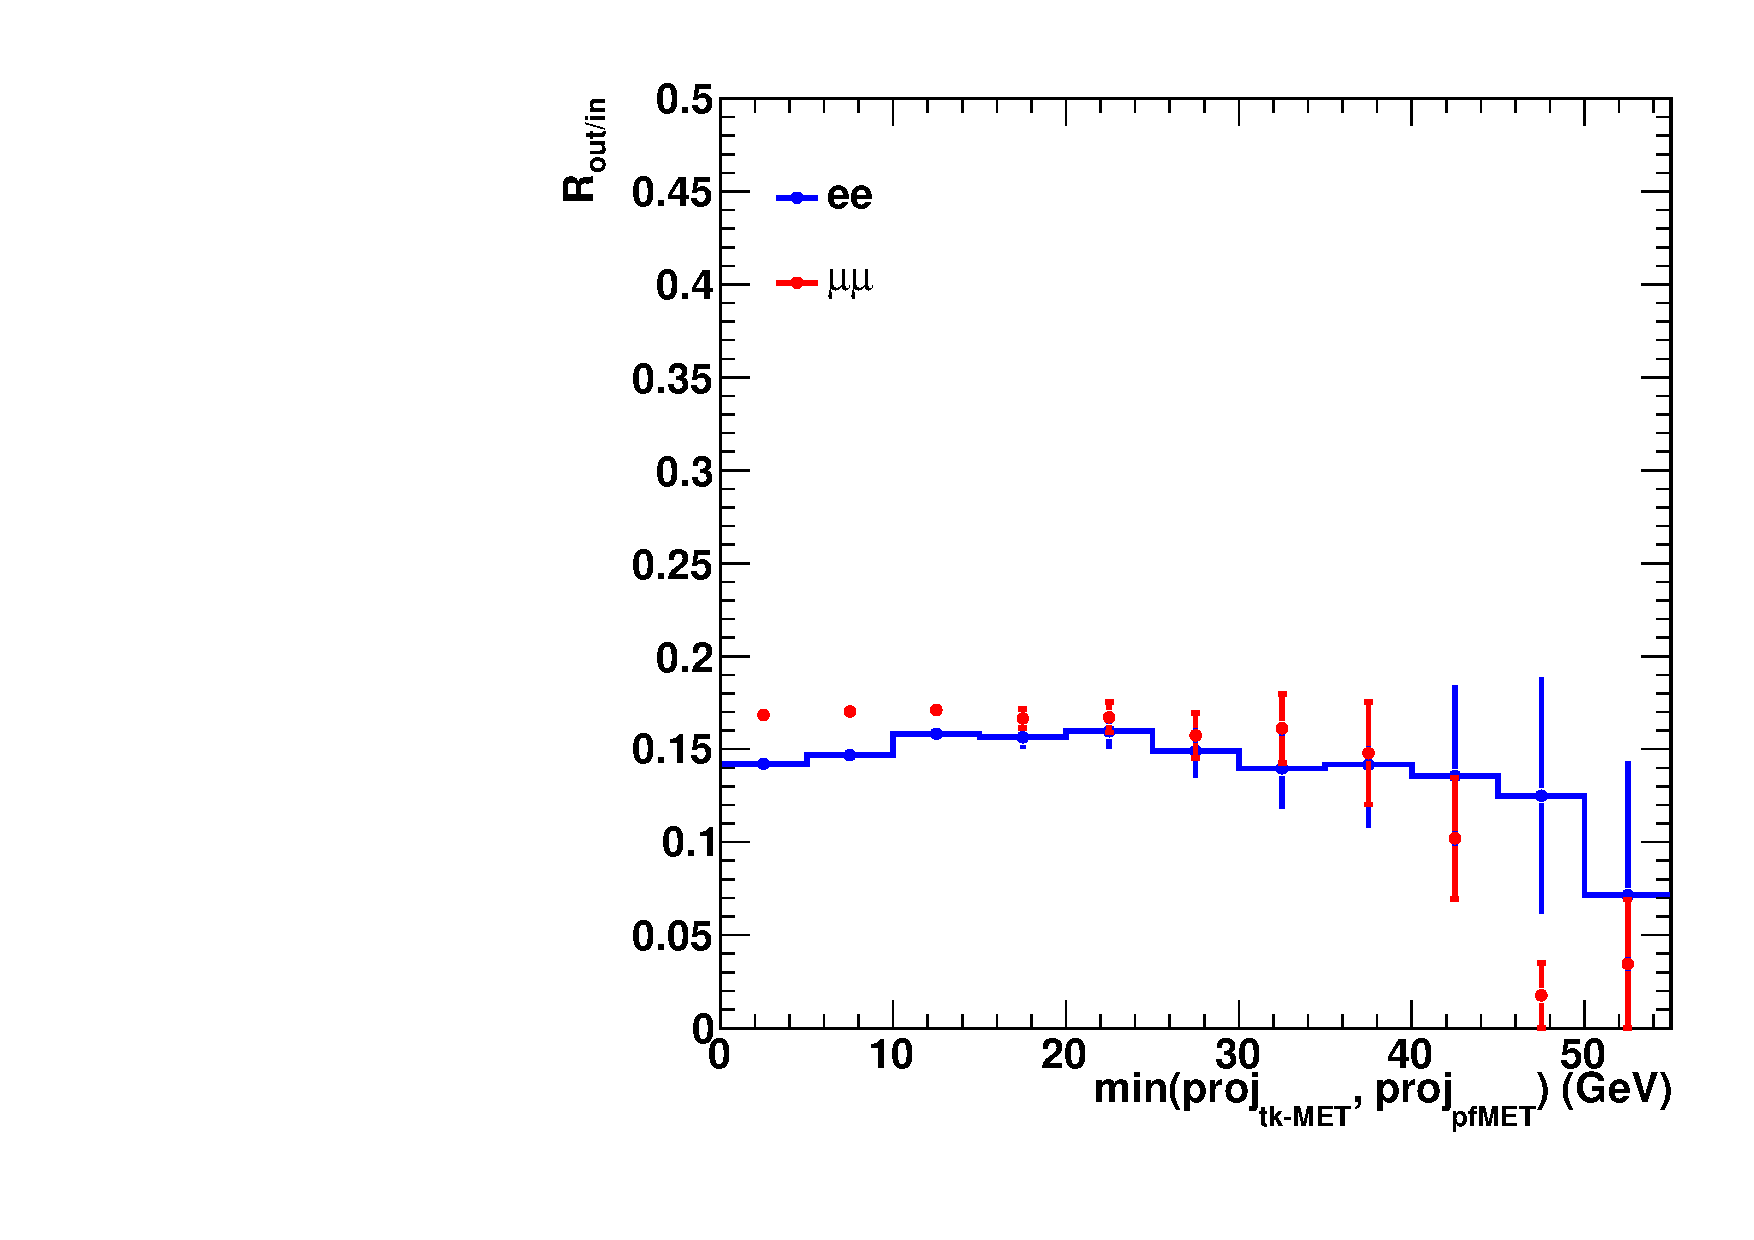
\includegraphics[width=0.3\textwidth]{figures/Routin_mc_1Jet.pdf}
%% 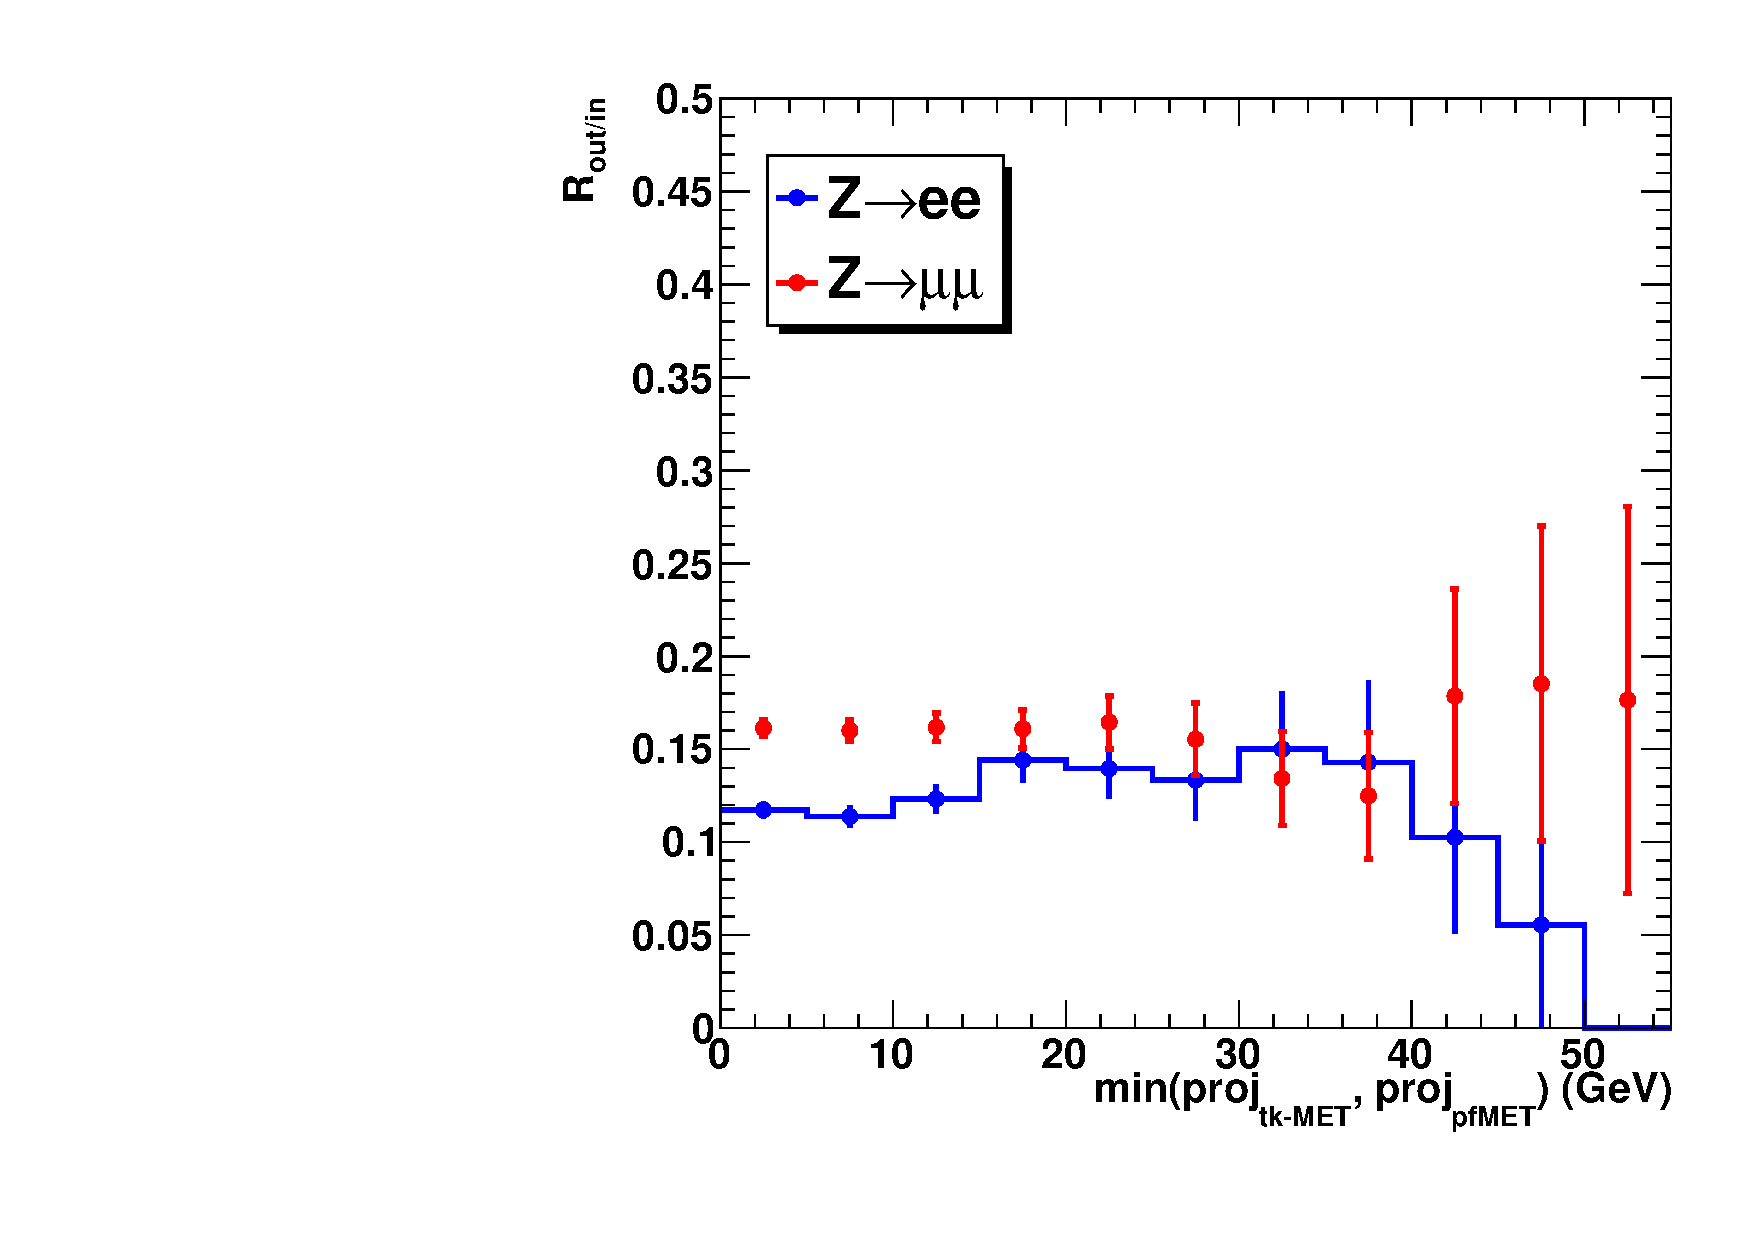
\includegraphics[width=0.3\textwidth]{figures/Routin_mc_2Jet.pdf}
%% \caption{ The ratio $R_{out/in}$ as a function of the $\met$ cut obtained using MC in the 
%% 0-Jet (left), 1-Jet (middle) and 2-Jet (right) bins. The event content in each 
%% bin is uncorrelated. The last bin represent the $R_{out/in}$ measured with min-MET $>$ 40 GeV. 
%% } %The difference in the ratio between 
%% %\ee\ and \mm\ final states is due to lower minimum muon momentum compared with electron
%% %(10 GeV vs 15 GeV), which allows for more low mass Drell-Yan events.}
%% \label{fig:routin_met}
%% \end{center}
%% \end{figure}
%% %%%%%%%%%%%%%%%%%%%%%%%%%%%%%%


%% %%%%%%%%%%%%%%%%%%%%%%%%%%%%%%
%% \begin{figure}[!htbp]
%% \begin{center}
%% 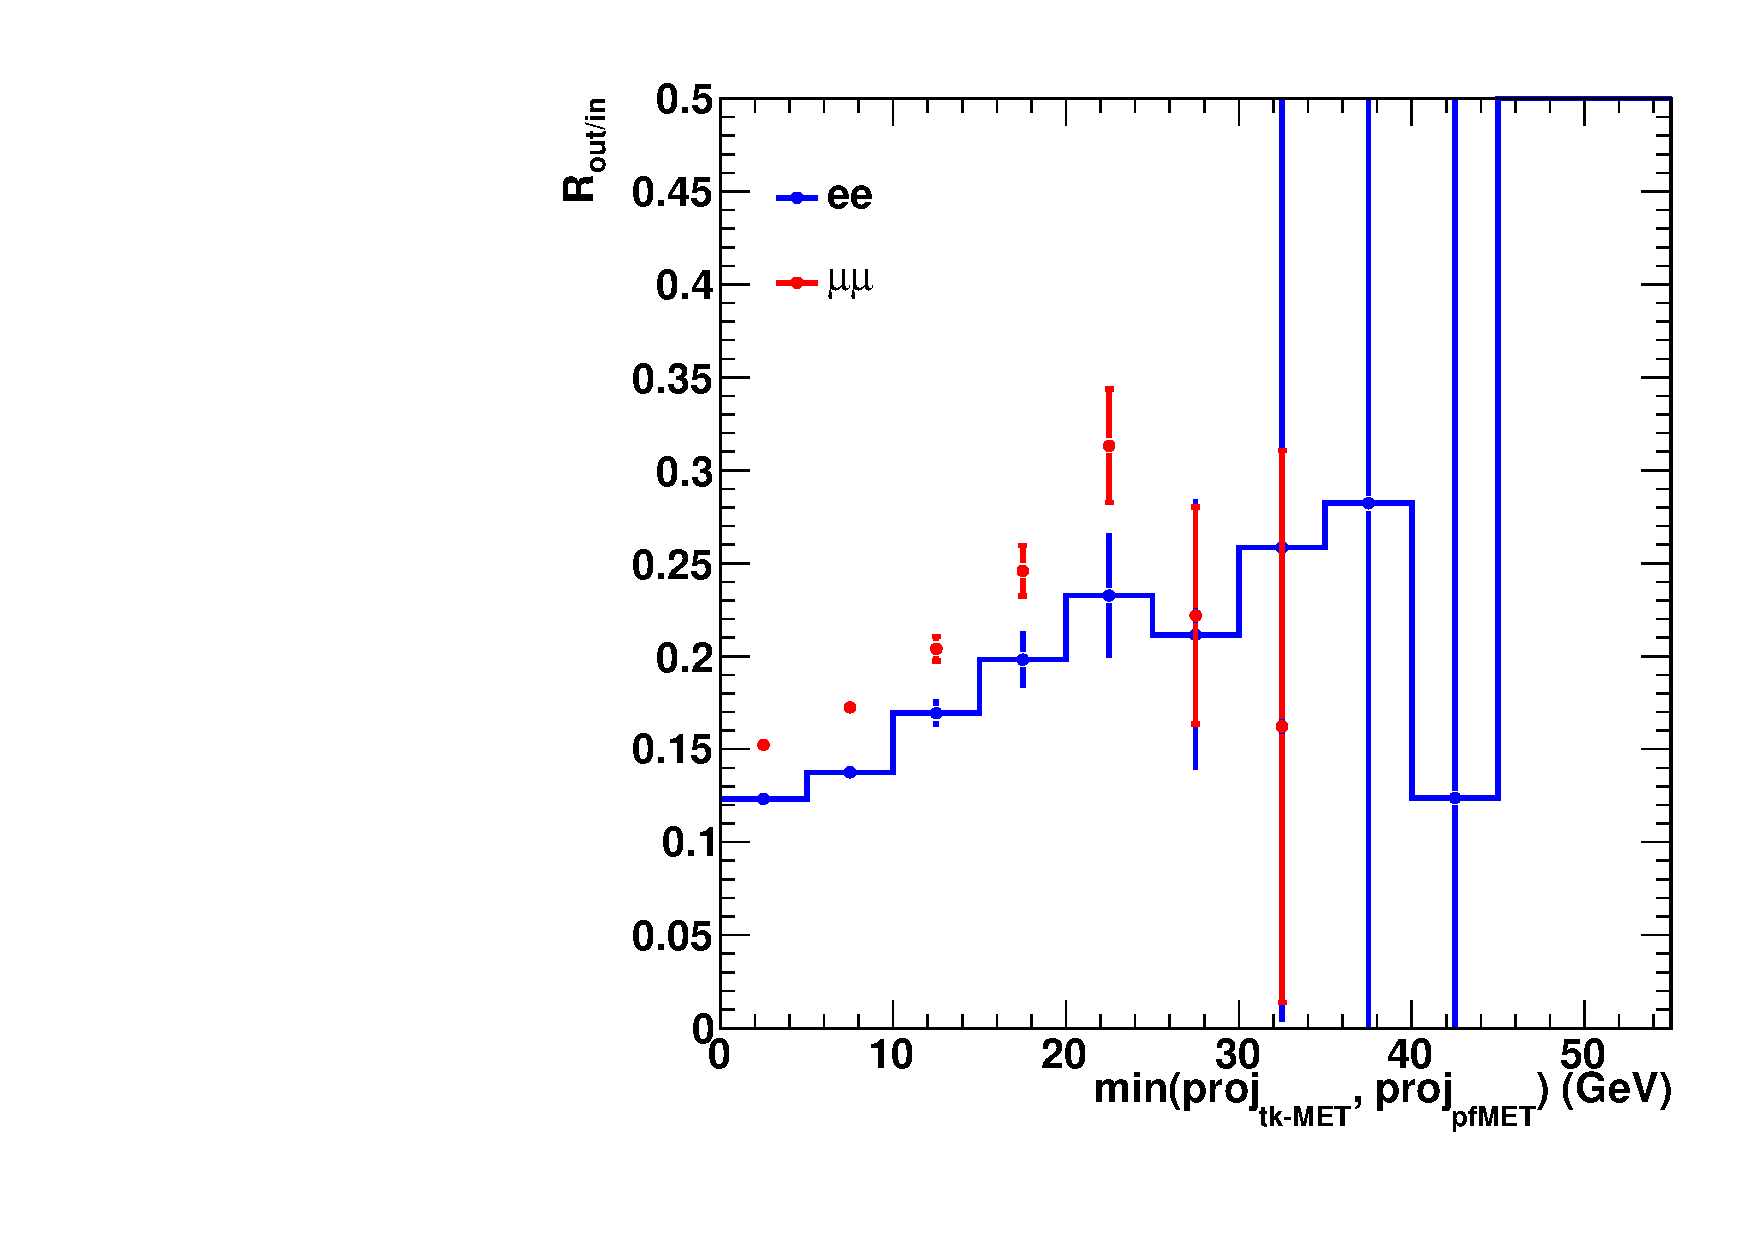
\includegraphics[width=0.3\textwidth]{figures/Routin_data_0Jet.pdf}
%% 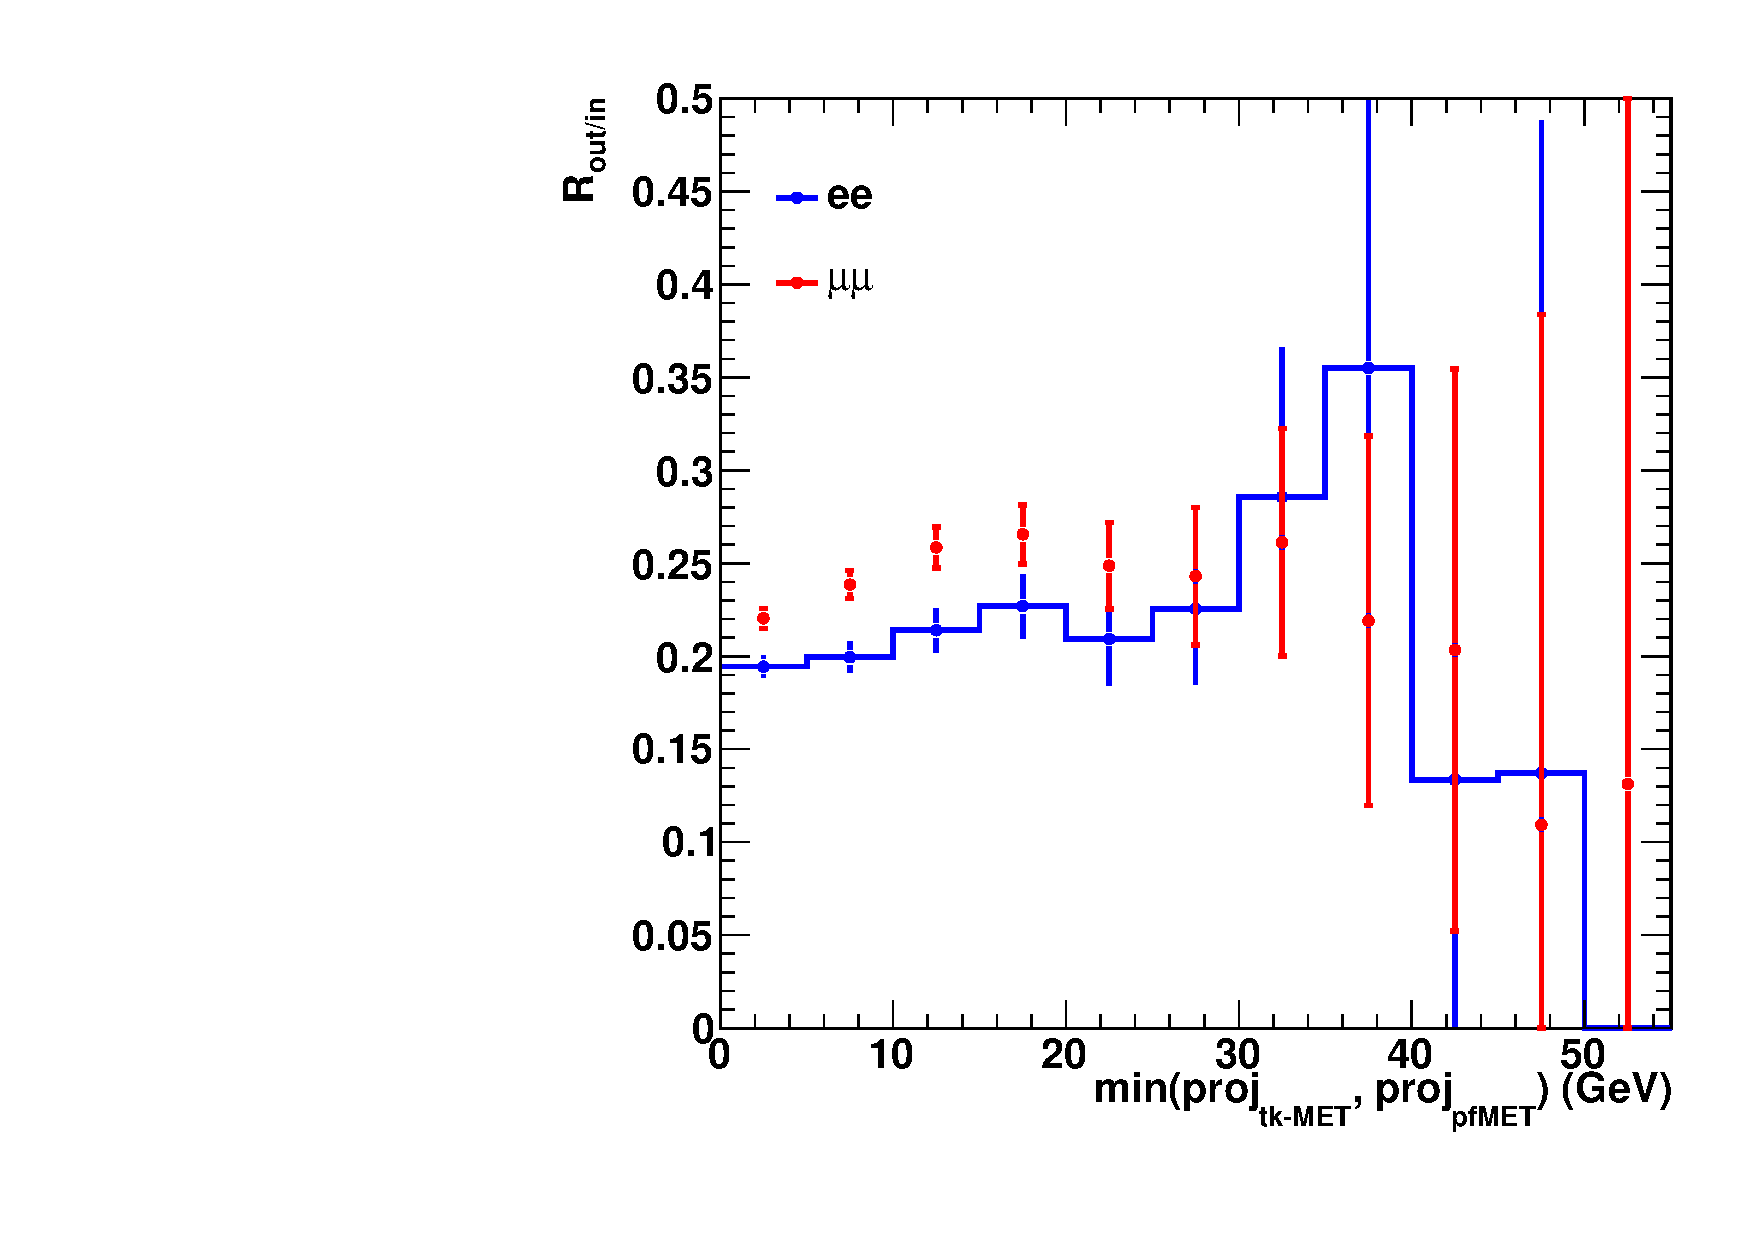
\includegraphics[width=0.3\textwidth]{figures/Routin_data_1Jet.pdf}
%% 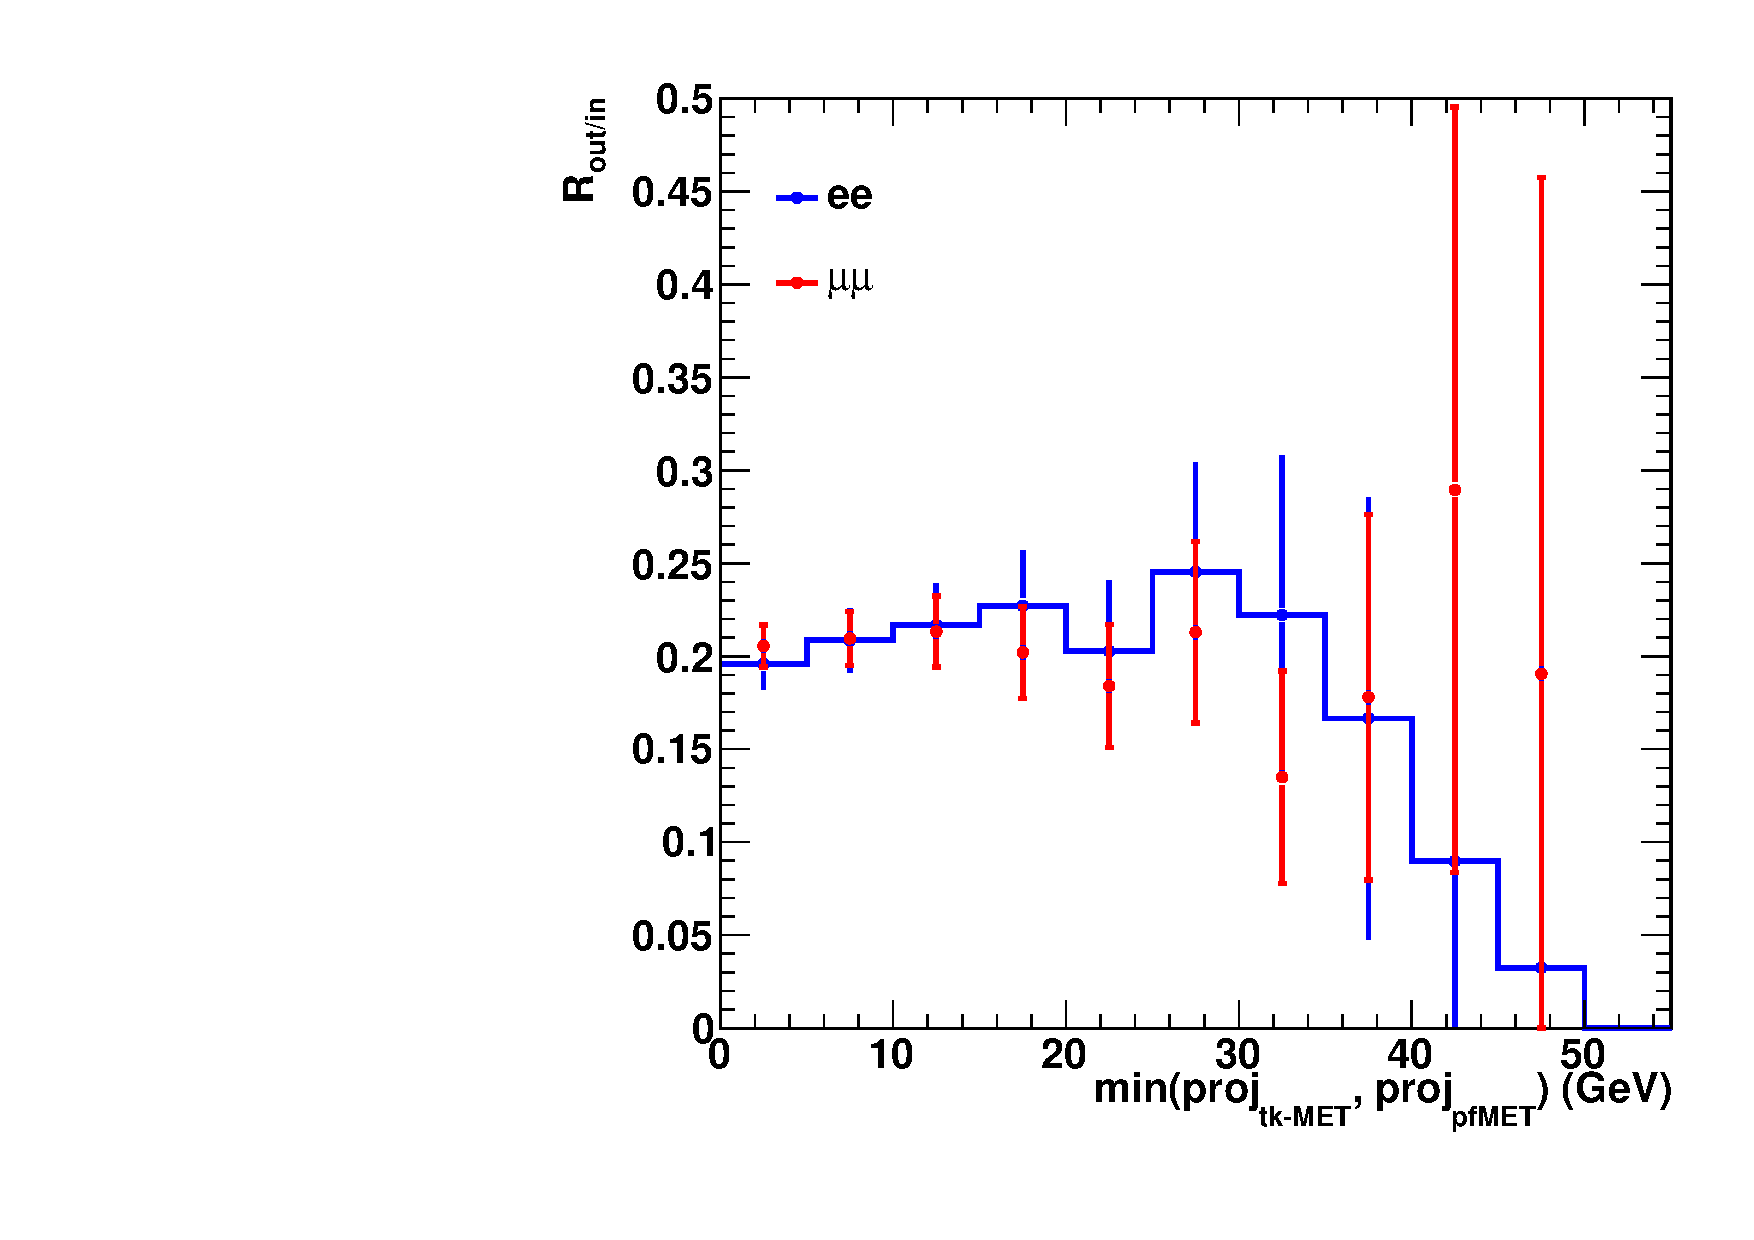
\includegraphics[width=0.3\textwidth]{figures/Routin_data_2Jet.pdf}
%% \caption{ The ratio $R_{out/in}$ as a function of the $\met$ cut obtained using data in the 
%% 0-Jet (left), 1-Jet (middle) and 2-Jet (right) bins. The event content in each 
%% bin is uncorrelated. The measurements are done only in the control region where min-MET $<$ 40 GeV, 
%% therefore the last bin is not filled. }
%% %The difference in the ratio between 
%% %\ee\ and \mm\ final states is due to lower minimum muon momentum compared with electron
%% %(10 GeV vs 15 GeV), which allows for more low mass Drell-Yan events.}
%% \label{fig:routin_met_data}
%% \end{center}
%% \end{figure}
%% %%%%%%%%%%%%%%%%%%%%%%%%%%%%%%


%% %% There are two ways in which the combination of DY and ZZ/ZW
%% %% backgrounds can be treated: one possibility is to use
%% %% equation \eqref{eq:dyest} for the combination of DY and peaking
%% %% ZZ/ZW background $(\textrm{Z} \to \ell\ell) +
%% %% (\textrm{W\!/Z} \to \textrm{any})$
%% %% %%%%%%%%
%% %% \begin{equation}\label{eq:dyExtrapM2}
%% %%   N(\ell\ell)_{\textrm{signal}} ^{\textrm{DY}+\textrm{ZV}} =
%% %%   (N(\ell\ell)_{\textrm{control}}^{\textrm{data}}-0.5\times
%% %%   N(e\mu)_{\textrm{control}} ^{\textrm{data}}\times k_{\ell\ell}
%% %%   ) \times R(\ell\ell)_{out/in}^{\textrm{DY}+\textrm{ZV}}
%% %% \end{equation}
%% %% %%%%%%%%%
%% %% and then add separately the non-peaking ZZ/ZW from simulation.  

%% The ZZ/ZW processes contribute to the events in the control region 
%% of the $m_{\ell\ell}$ region dominated by the DY. 
%% The contribution from ZZ/ZW becomes comparable to the Drell-Yan background 
%% after a tight projected \met selection of 40 GeV. 
%% The ZZ/ZW events contain natural \met, for which
%% the detector simulation is reliable\footnote{The ZZ/ZW events with
%% no \met are suppressed by the same large factor as the DY ones, and
%% therefore their contribution is as negligible at the level of the
%% final selection as it would be in the yield at the Z peak without \met
%% requirement.}. 
%% We subtract the expected peaking ZZ/ZW
%% contribution to the yield in the Z peak using the simulation in the 
%% estimation of number of events within the $Z$ window in data:
%% %The ZZ/ZW expectation is taken from simulation.
%% %the extrapolation from the subtracted yield, and then include the full
%% %ZZ/ZW expectation from simulation as a background of the analysis:
%% %%%%%%%%%%
%% \begin{equation}\label{eq:dyExtrapM3}
%%   N(\ell\ell)_{\textrm{signal}} ^{\textrm{DY}}=
%%   (N(\ell\ell)_{\textrm{control}}^{\textrm{data}}-0.5\times
%%   N(e\mu)_{\textrm{control}} ^{\textrm{data}}\times k_{\ell\ell}
%%   -N_{\textrm{control}}^{\textrm{ZV, sim.}} )  \times
%%   R(\ell\ell)_{out/in}^{DY}
%% \end{equation}
%% %%%%%%%%%%%%
%% %The subtraction using the simulation is legitimate since 
%% The ZZ/ZW contribution in the same flavor final states is then 
%% taken directly from simulation. 
%% Seperating the Drell-Yan and ZZ/WZ components 
%% accounts for the fact that the extrapolation from control 
%% region to signal region can be different for the two processes when
%% considering the full Higgs selection. We assume an overall 10\%
%% uncertainty on the ZZ/ZW yield in the peak, which is anyway
%% overshadowed by the statistical uncertainty on the observed events in
%% the Z peak in data.
%% % The second approach, that keeps the two components
%% %separate, This accounts for the fact that the extrapolation from control

%% The estimation from the on peak region relies on the assumption that
%% the dependence of the ratio $R_{out/in}$ on the $\met$ cut is well
%% modelled by the simulation and is relatively flat.
%% Figure~\ref{fig:routin_met} shows the ratios $R_{out/in}$ as functions
%% of the $\met$ cut at different jet bins determined from simulation at 
%% the \ww preselection level. The systematic uncertainty is assigned as the 
%% largest difference in the ratio to the central value as we vary the 
%% $\met$ cut from 0 to 40 GeV. 

%% We cross-checked the $R_{out/in}$ value in data.  Background processes
%% contribute equally to $ee$, $e\mu$, $\mu e$ and $\mu\mu$ final states
%% (after efficiency corrections), while Drell-Yan only contributes to
%% $ee$ and $\mu\mu$. Therefore we can subtract $e\mu$ and $\mu e$
%% contribtutions from $ee$ and $\mu\mu$ ones to get an estimate of
%% Drell-Yan.  Figure~\ref{fig:routin_met_data} shows the dependence of
%% $R_{out/in}$ of $\met$ cut evaluated in data.


%% %We then estimate the $R_{out/in}$ at a looser $\met$ selection
%% %($\met>$ 20 GeV) with respect the analysis one ($\met>$ 35 GeV).
%% %which allows not to run out of statistics in the $Z\to\ell\ell$ sample,
%% %both in case of simulation and data.

%% The value of $R_{out/in}$ changes as a function of the tight
%% kinematics requirements applied to select the Higgs signal region
%% (among which the tighter $\met$ cuts).  So we take the nominal value
%% from data estimation at the full Higgs selection, where no further
%% extrapolation is needed except the {\it in/out} region of the Z peak. 
%% To gain statistics, the $R_{out/in}$ is evaluated without applying the 
%% transverse mass cuts. 

%% We show the number of selected events in the Z peak region in data,
%% the correspondent value of $R_{out/in}$ and the comparison between the
%% expected DY contribution and the measured one in
%% Table~\ref{tab:routin_data_zeroj} and in Table~\ref{tab:routin_data_onej}
%% for zero and one jet bins, respectively. In the measurements we combine the 
%% $\zee$ and $\zmm$ contributions. 

%% %%%%%%%%%%%%%%%%%%%%%%%%%%%%%%
%% \begin{table}
%% \begin{center}
%% \begin{tabular}{c c c c c}
%% \hline
%% \vspace{-3mm} && \\
%% mass   & $N_{in}^{data}(DY)$ & $\langle R_{out/in} \rangle$ & $N_{out}^{data}(DY)$ & $N_{out}^{MC}(DY)$ \\
%% \vspace{-3mm} && \\
%% \hline
%% WW & 25.64 $\pm$ 13.24 & 0.25 $\pm$ 0.06 $\pm$ 0.05 & 6.46 $\pm$ 3.70 $\pm$ 1.16 & 2.00 $\pm$ 0.44 \\   
%% \hline
%% 120 GeV & 11.43 $\pm$ 6.33  & 0.28 $\pm$ 0.09 $\pm$ 0.76 & 3.24 $\pm$ 2.09 $\pm$ 8.71 & 0.81 $\pm$ 0.29 \\   
%% 130 GeV & 1.00 $\pm$ 4.07   & 0.73 $\pm$ 0.28 $\pm$ 1.08 & 0.73 $\pm$ 2.99 $\pm$ 1.08 & 0.93 $\pm$ 0.31 \\   
%% 140 GeV & 0.71 $\pm$ 3.93   & 0.59 $\pm$ 0.25 $\pm$ 0.63 & 0.42 $\pm$ 2.33 $\pm$ 0.44 & 0.56 $\pm$ 0.22 \\   
%% 150 GeV & 1.00 $\pm$ 4.32   & 0.40 $\pm$ 0.23 $\pm$ 0.27 & 0.40 $\pm$ 1.74 $\pm$ 0.27 & 0.25 $\pm$ 0.13 \\       
%% 160 GeV & 1.18 $\pm$ 2.02   & 1.00 $\pm$ 0.71 $\pm$ 0.64 & 1.18 $\pm$ 2.19 $\pm$ 0.76 & 0.25 $\pm$ 0.13 \\     
%% 170 GeV & 2.04 $\pm$ 2.67   & 1.00 $\pm$ 0.80 $\pm$ 0.70 & 2.04 $\pm$ 3.14 $\pm$ 1.43 & 0.19 $\pm$ 0.14 \\          
%% 180 GeV & 0.41 $\pm$ 3.21   & 0.57 $\pm$ 0.44 $\pm$ 0.16 & 0.24 $\pm$ 1.84 $\pm$ 0.07 & 0.12 $\pm$ 0.12 \\         
%% 190 GeV & 4.69 $\pm$ 4.65   & 0.33 $\pm$ 0.24 $\pm$ 0.23 & 1.56 $\pm$ 1.90 $\pm$ 1.08 & 0.12 $\pm$ 0.12 \\          
%% 200 GeV & 4.25 $\pm$ 5.40   & 0.14 $\pm$ 0.09 $\pm$ 0.08 & 0.59 $\pm$ 0.84  $\pm$ 0.34 & 0.12 $\pm$ 0.12 \\             
%% 250 GeV & 2.09 $\pm$ 6.52   & 0.03 $\pm$ 0.02 $\pm$ 0.02 & 0.06 $\pm$ 0.20 $\pm$ 0.03 & 0.06 $\pm$ 0.06 \\          
%% 300 GeV & 0.57 $\pm$ 4.56   & 0.05 $\pm$ 0.05 $\pm$ 0.39 & 0.03 $\pm$ 0.23 $\pm$ 0.22 & 0.06 $\pm$ 0.06 \\
%% \hline
%% \end{tabular}
%% \caption{The Drell-Yan estimation in the same flavor final state in the zero-jet bin.
%% \label{tab:routin_data_zeroj}}
%% \end{center}
%% \end{table}
%% %%%%%%%%%%%%%%%%%%%%%%%%%%%%%%



%% %%%%%%%%%%%%%%%%%%%%%%%%%%%%%%
%% \begin{table}
%% \begin{center}
%% \begin{tabular}{c c c c c}
%% \hline
%% \vspace{-3mm} && \\
%% mass   & $N_{in}^{data}(DY)$ & $\langle R_{out/in} \rangle$ & $N_{out}^{data}(DY)$ & $N_{out}^{MC}(DY)$ \\
%% \vspace{-3mm} && \\
%% \hline
%% WW & 50.73 $\pm$ 10.69 & 0.15 $\pm$ 0.03 $\pm$ 0.10 & 7.39 $\pm$ 2.08 $\pm$ 5.11 & 3.24 $\pm$ 0.56 \\
%% \hline
%% 120 & 14.21 $\pm$ 4.01 & 0.07 $\pm$ 0.02 $\pm$ 0.23 & 0.96 $\pm$ 0.39 $\pm$ 3.24 & 0.87 $\pm$ 0.29 \\
%% 130 & 4.02 $\pm$ 2.66  & 0.13 $\pm$ 0.03 $\pm$ 0.41 & 0.51 $\pm$ 0.37 $\pm$ 1.64 & 1.06 $\pm$ 0.32 \\
%% 140 & 3.82 $\pm$ 2.66  & 0.11 $\pm$ 0.03 $\pm$ 0.26 & 0.43 $\pm$ 0.33 $\pm$ 1.00 & 1.06 $\pm$ 0.31 \\
%% 150 & 12.45 $\pm$ 4.26 & 0.08 $\pm$ 0.03 $\pm$ 0.15 & 0.94 $\pm$ 0.47 $\pm$ 1.90 & 0.56 $\pm$ 0.21 \\
%% 160 & 3.27 $\pm$ 3.20  & 0.23 $\pm$ 0.09 $\pm$ 0.32 & 0.75 $\pm$ 0.79 $\pm$ 1.03 & 0.56 $\pm$ 0.21 \\
%% 170 & 4.23 $\pm$ 3.35  & 0.23 $\pm$ 0.09 $\pm$ 0.22 & 0.97 $\pm$ 0.86 $\pm$ 0.92 & 0.37 $\pm$ 0.18 \\
%% 180 & 2.88 $\pm$ 3.51  & 0.18 $\pm$ 0.07 $\pm$ 0.10 & 0.52 $\pm$ 0.66 $\pm$ 0.28 & 0.31 $\pm$ 0.16 \\
%% 190 & 11.37 $\pm$ 4.73 & 0.08 $\pm$ 0.03 $\pm$ 0.13 & 0.94 $\pm$ 0.51 $\pm$ 1.47 & 0.44 $\pm$ 0.21 \\
%% 200 & 17.17 $\pm$ 5.61 & 0.07 $\pm$ 0.02 $\pm$ 0.08 & 1.15 $\pm$ 0.55 $\pm$ 1.36 & 0.44 $\pm$ 0.21 \\
%% 250 & 23.42 $\pm$ 6.39 & 0.07 $\pm$ 0.02 $\pm$ 0.01 & 1.67 $\pm$ 0.70 $\pm$ 0.31 & 0.75 $\pm$ 0.28 \\
%% 300 & 17.66 $\pm$ 5.04 & 0.05 $\pm$ 0.02 $\pm$ 0.07 & 0.90 $\pm$ 0.51 $\pm$ 1.30 & 0.37 $\pm$ 0.20 \\     
%% \hline
%% \end{tabular}
%% \caption{The Drell-Yan estimation in the same flavor final state in the one-jet bin.
%% \label{tab:routin_data_onej}}
%% \end{center}
%% \end{table}
%% %%%%%%%%%%%%%%%%%%%%%%%%%%%%%%

%% The method to estimate the Drell-Yan background performed for each
%% Higgs mass point is the most robust because it allows to do the
%% estimation directly on the signal kinematics region through a proper
%% estimation of $R_{out/in}$.  It leads to fairly large uncertainties on
%% the background mostly dominated by small event count in the Z-peak
%% area (see Appendix~\ref{app:dy_writeup}). It does not affect the mass points where we have sensitivity to
%% the Standard Model Higgs with current amount of data. 
%% With more data the uncertainties on the background estimation should improve.


%   \subsection{$\wgamma^*$ Background}
%     \label{sec:bkg_wgammastar}
%     The electroweak process \Wgstar\ is normally covered in Monte Carlo
simulations as a part of the \WZ\ process. Questions were raised if
the low mass region is adequately covered since the \WZ\ Madgraph
simulations have a generator level cut $m_{\gamma^*}>12$ and there is
significant rate of events at lower values~\cite{wgstar}.  \WZ\
and \Wgstar\ processes contribute as background to the Higgs signal in
the case one of the three leptons in the final state is not
detected. We have simulated the low mass part of \Wgstar\ using a
leading order matrix element Monte Carlo (Madgraph). The generator
level selection requirements were relaxed: require two leptons each
with $\pt>5$~\GeV{} with no restrictions on the third one, consider
electrons and muons to be massive to properly simulate the kinematic
cutoff. The key question is to observe the process in data and
validate the simulation. In particular we need to measure the
cross-section of the process to have reliable predictions for the
background outside the control region.

We can consider separately the two cases where the lepton pair from
the \Astar are electrons or muons. For the generator level selections
mentioned above the cross section for
the \ensuremath{l^{\pm}e^{+}e^{-}} final state
(with \ensuremath{l^{\pm}}=\ensuremath{\mu^{\pm}}
or \ensuremath{e^{\pm}} being the lepton from the \W\ decay) is larger
by a factor $\sim3$ with respect to
the \ensuremath{l^{\pm}\mu^{+}\mu^{-}} case due to the lower
production threshold (defined by \ensuremath{2M_{l}}) and the steep
rising of \ensuremath{d\sigma/dM_{\gamma}}.  The leptons originated
from the virtual photon feature small opening angle and small
invariant mass.  At least one of the two leptons is soft with an
average \pt\ of $\sim5$ GeV.  In the \ensuremath{l^{\pm}e^{+}e^{-}}
case the way of faking the signal is similar to the \wgamma\
background when the photon converts in the material close to the
interaction vertex (it can be seen as a sort of ``prompt''
conversion).  For the \ensuremath{l^{\pm}\mu^{+}\mu^{-}} final state,
the low \pt\ of the softest muon often prevents it from reaching the
muon stations and thus to be identified as a muon.

To measure the production rate of \Wgstar\ in data we focused only on
the \ensuremath{l^{\pm}\mu^{+}\mu^{-}} final state, since the large
background from QCD makes it hard to extract signal in
the \ensuremath{l^{\pm}e^{+}e^{-}} case.  The \Wgstar\ control region
selection has been optimized for high purity.  The following
selections have been applied:
\begin{itemize}
\item 
the muon pair associated to the virtual photon needs to have opposite
charge. In the case of \ensuremath{\mu\mu\mu} final state, the pair
with lowest mass is assumed to originate from the \Astar.
\item 
the muon isolation is redefined to exclude muons from the isolation
energy calculation to reconstruct events with two muons closer
than \delR=0.3.
\item 
to suppress top background events with less than 2 jets are
considered and anti b-tagging is required for all jets
with \ensuremath{p_\mathrm{T}>10} GeV.
\item 
to suppress QCD background minMet$>20$ and \mt$>20$ (where \mt is
computed from the \W's lepton and the \met).
\item 
\ensuremath{M_{\mu\mu}<12} GeV.
\end{itemize} 

The upper bound on the di-muon mass is set to get rid of the
interference between \Wgstar\ and \ensuremath{\W\Zstar}.  The Monte
Carlo used for the \WZ\ process includes both \Astar\ and \Zstar\
contributions and takes properly into account the interference between
them.  The plot in Figure \ref{fig:WgammaStarMass} compares the mass
distributions of the muon pair associated with the virtual photon for
data and Monte Carlo once all the selections listed above are applied
but \ensuremath{M_{\mu\mu}<12} GeV.  The data correspond to an
integrated luminosity equal to 2.97\ifb.

\begin{figure}[hbt]
\begin{center}
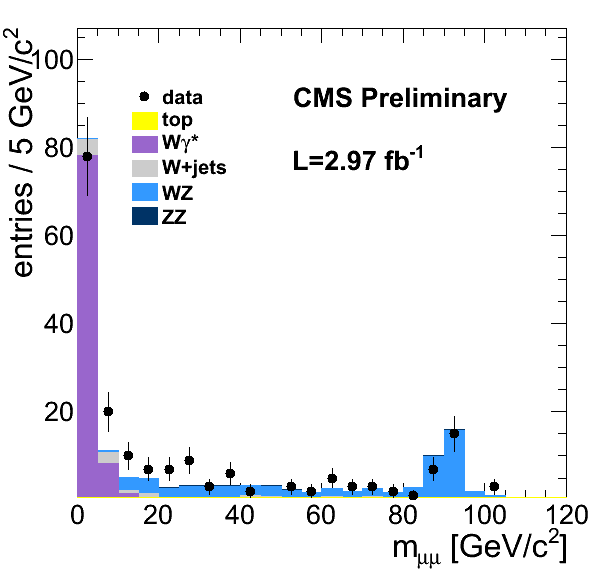
\includegraphics[width=0.5\linewidth]{figures/gammaMass_m120.png} 
\caption{\label{fig:WgammaStarMass}\protect Comparison of data and Monte Carlo for  
mass distributions of the muon pair associated with the virtual
photon.  All the selections defining the \Wgstar\ control region are
applied but \ensuremath{M_{\mu\mu}<12} GeV.}
\end{center}
\end{figure}

The plots in Figure \ref{fig:WgammaStar}, displaying data and MC
distributions for the muon pair associated with the virtual photon,
(left: opening angle, center: di-muon mass, right: \pt\ of the softest
muon) assess the compatibility of the data belonging to the control
region with the expectations from the \Wgstar\ Monte Carlo.  
The contribution from other backgrounds is very limited, 
the only process which is not completely negligible is $\Wjets$
which is computed directly from data by means of the fake rate
method described in section \ref{sec:bkg_fakes}.
A small difference is observed between the data and MC shapes
for the mass of the virtual photon candidate; 
as this mismodelling was also observed in 2011 data we will discuss the
related systematics in the following.

\begin{figure}[hbt]
\begin{center}
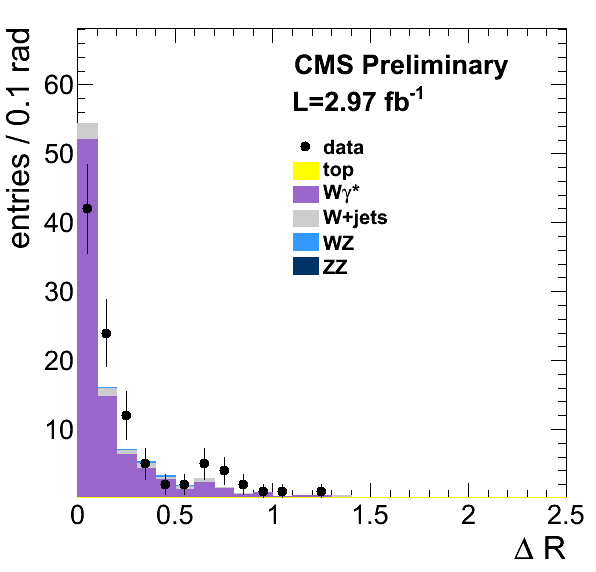
\includegraphics[width=0.3\linewidth]{figures/gammaDR_m12.png} 
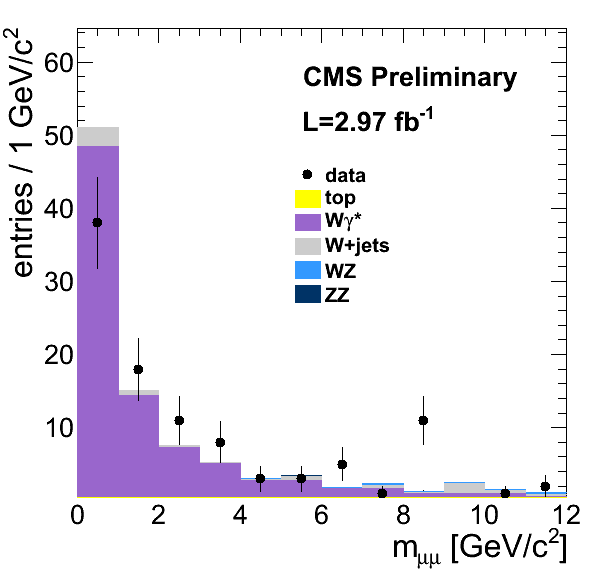
\includegraphics[width=0.3\linewidth]{figures/gammaMass_m12.png}
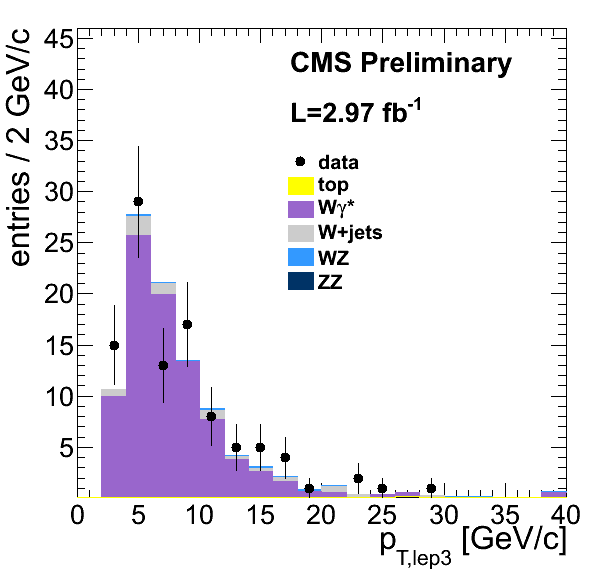
\includegraphics[width=0.3\linewidth]{figures/gammaLep3Pt_m12.png}
\caption{\label{fig:WgammaStar}\protect Comparison of data and Monte Carlo for three 
main distributions of the muons associated with the virtual photon in
the \Wgstar~ control region.  Left: opening angle (\delR).  Center:
di-muon mass.  Right:. softest muon \pt.}
\end{center}
\end{figure}

\begin{table}[!hbt]
\begin{center}
\begin{tabular}{|c|c|c|c|c|c|c|}
\hline
& \multicolumn{2}{|c|}{\ensuremath{e\mu\mu}} & \multicolumn{2}{|c|}{\ensuremath{\mu\mu\mu}} & \multicolumn{2}{|c|}{\ensuremath{l\mu\mu}} \\
\hline
& SS & OS & SS & OS & SS & OS \\
\hline
data yields & 12 & 17 & 35 & 37 &  49 &  52\\
\hline
background & 1.8 & 1.0 & 2.3 &  3.4 &  5.2 & 3.3\\
\hline
(raw) \Wgstar~ MC yields & $7.7 \pm 0.5$ & $7.7 \pm 0.4$ & $20.1 \pm 0.7$ & $22.9 \pm 0.8$ & $30.6 \pm 0.9$ & $27.8 \pm 0.8$ \\
\hline
\hline
{\em k-}factor & \multicolumn{2}{|c|}{1.69} & \multicolumn{2}{|c|}{1.54} & \multicolumn{2}{|c|}{1.58} \\
\hline
\end{tabular}
\caption{Results of the measurements in the \Wgstar control region.
{\em k-}factors are computed as ratios between the data yields and the
MC predictions.  Results are shown separately for \ensuremath{e\mu\mu}
and \ensuremath{\mu\mu\mu} final states in the first two columns,
whereas the third one consider them together.  
For each final state yields are shown separately for same sign and opposite sign
of the two highest \pt leptons. 
The data yields correspond to \ensuremath{L=2.97\ifb}.
\label{tab:wgamma}}
\end{center}
\end{table}

Table \ref{tab:wgamma} summarizes the results of the \Wgstar~
measurement and the normalization of the corresponding Monte
Carlo. The measured {\em k}-factor is 1.6 and it is fully consistent with
the one measured with the 2011 dataset ~\cite{HWW2011}.
The {\em k}-factors measured for other EWK processes computed at the leading
order resulted very similar to the one obtained here, giving therefore 
further confidence on the accuracy of the Monte Carlo simulation.  
As a further cross check, the event yields for same sign and opposite sign 
(where the pair of highest \pt leptons is considered) have been looked at in data:
as shown in table \ref{tab:wgamma}, a very good agreement is observed for each final 
state.

To estimate the systematic uncertainty related to the data versus Monte Carlo 
disagreement on the virtual photon mass shape (most likely due to mismodeling
of reconstruction efficiency of close-by muon one of which at very low \pt),
the scale factor has been computed in sub-regions of the mass spectrum and compared to what
obtained from the full range. 
We performed the same analysis on 2011 data obtaining almost identical results as
from the 2012 dataset (four scale factors estimations): 
the scale factor in the [0-2] GeV mass range results smaller ($\sim1.3$),
whereas in the range [2-12] it results larger ($\sim2.2$).
To account for this effect we assign a systematic uncertainty corresponding to
the average of the spreads of the fours estimates w.r.t the central value, obtaining
an error of $0.25\%$. 



%   \subsection{Other Backgrounds}
%     \label{sec:bkg_other}
%     The $WZ$ and $ZZ$ events with lepton pairs from a resonant $Z$ boson are suppressed 
by the $Z$ veto. The remaining contribution is estimated from simulation, 
after applying the proper data to simulation correction factors for the 
lepton and trigger efficiencies. 
%

The $W+\gamma$ background, where the $\gamma$ fakes an electron through
an asymmetric conversion is difficult to estimate from data. Additional
cross-checks can be performed to place data based constraints on this estimate. 
For instance, applying the same standard selection, but requiring two same-sign 
leptons, gives a sample dominated by $\Wjets$ and $W+\gamma$ events. Again, the 
expected contribution is very small, due to stringent $\gamma$ conversion 
requirements explained in Sec.~\ref{sec:sel_electrons}.

The electroweak process \Wgstar\ enters the signal region if one of the leptons 
from the $\gamma^*$ is lost. This background is normally covered in Monte Carlo
simulations as a part of the \WZ\ process. However in the simulation, 
there is a generator level cut of $m_{\gamma^*}>12$ GeV, and there is
a significant rate of events at lower values~\cite{wgstar}. 
A dedicated $W\gamma^*$ sample is simulated in Madgraph 
with $m_{\gamma^*} < 12$ GeV. The prediction from this simulation is then normalized to 
data according to the rate in the $W\gamma^*$ enriched region, as 
detailed in Ref.~\cite{HWW2011Final}. 
The normalization factor applied is 1.53.


The $\dytt$ background is suppressed signficiantly by the 
projected $\met$ requirements as the $\met$ tend to be aligned with 
one of the leptons. However the large amount of pileup interactions 
may lead to fake \met\ that is larger than the natural \met\
in \dytt\ events. Given that the fake \met\ can not be reliably 
estimated in simulation, we developped two data-driven methods to estimate the 
$\dytt$ background as documented in Ref.~\cite{HWW2011Final}. 
Both methods find that the \dytt\ rate in data is a factor of 4 larger than 
the value predicted by simulation. 



\section{Pileup Reweighting}
     \label{sec:pileupReweighting}
      Due to the fast evolution of the LHC machine, with a rapid rise in the
instantaneous luminosity, the data taking conditions have changed
rapidly.  In particular it is difficult to exactly reproduce the
number of overlapping events (i.e. pile-up) between data and
simulation, and thus there will be differences in the number of
reconstructed primary vertices. We correct this disagreement by
reweighting the simulation to match the number of pileup events in data. 

The target pileup distribution for data is generated using the instantaneous luminosity 
per bunch crossing for each luminosity section, stored in the LumiDB database, 
and the total pp inelastic cross section of $68$mb, integrated over the 
full data-taking period. A poissonian smearing is applied to model
statistical fluctuations in the actual number of pileup events 
present in the data. The source distribution is taken from the PileupInfo
collection which stores the true number of pileup events mixed with the 
particular hard interaction process in each Monte Carlo event. Comparisons of the
pileup distribution from the Summer11 Monte Carlo samples and the pileup 
distribution from various periods of data-taking is shown in Figure 
\ref{fig:NPU}. The resulting weighting factors are shown in Figure 
\ref{fig:PUReweightingFactors}. 

 
\begin{figure}[hbt]
\begin{center}
%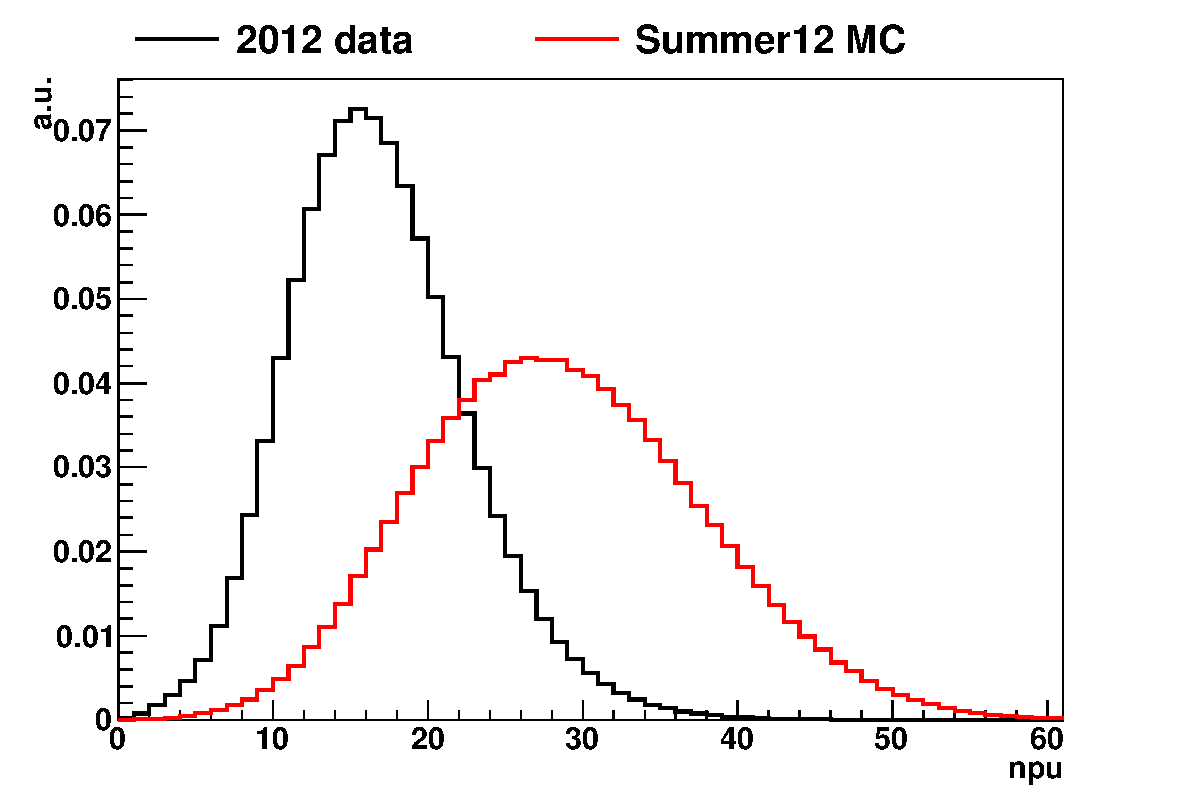
\includegraphics[width=0.7\linewidth]{figures/NPUDistributions.pdf}
\caption{\label{fig:NPU} Comparison of the number of pileup interactions 
for the Monte Carlo and various periods of 2011 data.}
\end{center}
\end{figure}

\begin{figure}[hbt]
\begin{center}
%\includegraphics[width=0.7\linewidth]{figures/ReweightingFactors.pdf}
\caption{\label{fig:PUReweightingFactors} Pileup reweighting factors for various periods of 2011 data.}
\end{center}
\end{figure}


A cross check of this procedure is performed by comparing the number of 
reconstructed primary vertices and the event energy density ($\rho$)
from \zmm\ events in data and Monte Carlo. The comparisons are shown in
Figures \ref{fig:PUValidation_Run2011A},\ref{fig:PUValidation_Run2011B},
and \ref{fig:PUValidation_Full2011} for Run2011A, Run2011B, and the 
total 2011 combined data, respectively. The residual differences 
reflect the size of the systematic uncertainty in the determination 
of the amount of pileup present in the data. Since the dependence 
of the efficiencies for selecting signal and background events on 
pileup are small, this systematic uncertainty due to the pileup 
is small when propagated to the final 
result.

\begin{figure}[hbt]
\begin{center}
%\subfigure[Number of reconstructed vertices]{\includegraphics[width=0.45\linewidth]{figures/PileupReweightingValidation_NVtx_SmurfV6DYmm_Run2011A.pdf}}
%\subfigure[Event energy density ($\rho$)]{\includegraphics[width=0.45\linewidth]{figures/PileupReweightingValidation_Rho_SmurfV6DYmm_Run2011A.pdf}}
\caption{\label{fig:PUValidation_Run2011A} Number of reconstructed primary vertices (a) and
the event energy density (b) for data and Monte Carlo reweighted in the number
of pileup events for the Run2011A dataset.}
\end{center}
\end{figure}

\begin{figure}[hbt]
\begin{center}
%\subfigure[Number of reconstructed vertices]{\includegraphics[width=0.45\linewidth]{figures/PileupReweightingValidation_NVtx_SmurfV6DYmm_Run2011B.pdf}}
%\subfigure[Event energy density ($\rho$)]{\includegraphics[width=0.45\linewidth]{figures/PileupReweightingValidation_Rho_SmurfV6DYmm_Run2011B.pdf}}
\caption{\label{fig:PUValidation_Run2011B} Number of reconstructed primary vertices (a) and
the event energy density (b) for data and Monte Carlo reweighted in the number
of pileup events for the Run2011B dataset.}
\end{center}
\end{figure}

\begin{figure}[hbt]
\begin{center}
%\subfigure[Number of reconstructed vertices]{\includegraphics[width=0.45\linewidth]{figures/PileupReweightingValidation_NVtx_SmurfV6DYmm_Full2011.pdf}}
%\subfigure[Event energy density ($\rho$)]{\includegraphics[width=0.45\linewidth]{figures/PileupReweightingValidation_Rho_SmurfV6DYmm_Full2011.pdf}}
\caption{\label{fig:PUValidation_Full2011} Number of reconstructed primary vertices (a) and
the event energy density (b) for data and Monte Carlo reweighted in the number 
of pileup events for the full 2011 dataset.}
\end{center}
\end{figure}



\section{Efficiency Measurements}
     \label{sec:alleff}
     \subsection{Lepton Efficiency}
     \label{sec:efficiency}
      
We used the tag and probe method on \dyll~events to provide an unbiased, high-purity, 
lepton sample with which to measure both online and offline selection efficiencies.
This method, which is now described, 
has been used successfully in previous CMS analyses \cite{ref:tagprobe_mit_w}\cite{ref:tagprobe_snt_top}.

\subsubsection{Method}
For both electrons and muons we used the lowest threshold unprescaled single trigger sample
available in the Prompt Reco.  This corresponds to:

\begin{itemize}
    \item Muons: HLT\_IsoMu24\_eta2p1\_v*
    \item Electrons: HLT\_Ele27\_WP80\_v*
\end{itemize}

At least one of the leptons, the {\it tag}, was required to pass the full selection criteria
while the other lepton, the {\it probe}, was required to pass a set of identification criteria leaving 
it unbiased with respect to the criterion under study. By requiring that the tag was able to have passed 
the single lepton trigger on which the events were acquired, we reduced the bias due to the trigger on 
the probe. Also, the tight criteria imposed on the tag coupled with the invariant mass requirement 
improves the purity of the sample. 

To reduce the background to the offline selection measurements,
the selections were split into the ID and isolation parts.  
The efficiency of the ID part was measured with respect to the isolation
requirements, and vice versa, in both data and simulation.
This is referred to as the N-1 method.
The bias on the efficiency from changing the denominator is
expected to be negligible is the scale factors for each step used
are close to one.
To estimate and subtract any residual background contribution in the data measurements,
a simultaneous fit was performed to the mass distributions
of passing and failing probes in the range $60<M_{ll}<120$ GeV.
The signal model for electrons was taken from simulation, 
with a gaussian smearing component to take into account the resolution.
The background model is an exponential times an error function.
In the simulation measurements, simple counting was used.
This method and its associated systematics are discussed in detail in Reference \cite{ref:tagprobe_mit_w}
The trigger efficiency is measured with respect to the full offline selection,
and thus the probe sample is very pure.  In this case the efficiencies were
extracted by simple counting in the mass range $81<M_{ll}<101$ GeV.

To produce overall data-MC scale factors to apply in the analysis, we factorise the efficiency measurements
into two steps such that

\begin{equation}
\varepsilon_{total} = \varepsilon_{offline} \times \varepsilon_{trigger}.
\end{equation}

The offline efficiency $\varepsilon_{offline} = \varepsilon_{offline}^{l1} \times \varepsilon_{offline}^{l2}$
is the product of the efficiencies of the two leptons and is discussed in more detail in Sections \ref{sec:eff_electron}
and \ref{sec:eff_muon} for electrons and muons respectively.
The trigger efficiency is measured with respect to the offline selection and
is discussed in more detail in Section \ref{sec:eff_trigger}.


	 \subsubsection{Electron Efficiency}
	 \label{sec:eff_electron}
	 
The electron selection efficiency can be factorised into two contributions,
the efficiency from the electron reconstruction and from the additional
analysis selections that are described in Section~\ref{sec:sel_electrons}.

The electron reconstruction efficiency is defined as the efficiency for a
supercluster to be matched to a reconstructed ECAL driven GSF electron.
The data to simulation scale factor was measured for the W and Z cross-section
analysis~\cite{VBTFCrossSectionNote}~\cite{ref:tagprobe_mit_w},
and found to be consistent with $1.0$ with a total uncertainty of
$1.3\%$ and $1.5\%$ for the barrel and endcap, respectively.

We thus measure the efficiency of our offline analysis selection 
with respect to a reconstructed ECAL driven GSF electron denominator. 
The resulting data to simulation scale factors are given in Table~\ref{tab:eff_ele_offline}.

\begin{table}[!ht]
\begin{center}
\begin{tabular}{c|c|c}
\hline
Measurement & Barrel ( $|\eta|<1.479$ )   & Endcap ( $|\eta|>1.479$ )  \\ 
\hline
$  10<p_T<  15$ & 0.87 $\pm$ 0.05  & 0.79 $\pm$ 0.08  \\ \hline 
$  15<p_T<  20$ & 0.94 $\pm$ 0.02  & 0.90 $\pm$ 0.04  \\ \hline 
$  p_T > 20 $ & 0.98 $\pm$ 0.00  & 0.97 $\pm$ 0.00  \\ \hline 
\end{tabular}
\caption{Offline selection scale factors for electrons.}
\label{tab:eff_ele_offline}
\end{center}
\end{table}


	 \subsubsection{Muon Efficiency}
	 \label{sec:eff_muon}
	 
The muon selection efficiency and the resulting data to simulation
scale factors are estimated using a similar method to the electron efficiency.
Since the muon reconstruction was proved to be well modeled in the simulation~\cite{VBTFCrossSectionNote}
we test only the analysis selection part.

We measure the muon selection efficiency with respect to a reconstructed Global muon
denominator.
% in the
%following four detector regions according to $\eta$: barrel ($|\eta|<0.8$),
%overlap region between DT and CSC ($0.8<|\eta|<1.2$), endcaps ($1.2<|\eta|<2.1$) and
%most forward region ($2.1<|\eta|<2.4$).
The resulting data to simulation scale factors are given in Table \ref{tab:eff_mu_offline}.

\begin{table}[!ht]
\begin{center}
\begin{tabular}{c|c|c}
\hline
Measurement & Barrel ( $|\eta|<1.479$ )   & Endcap ( $|\eta|>1.479$ )  \\ 
\hline
<<<<<<< eff_muon.tex
$  10<p_T<  15$ & 0.93 $\pm$ 0.02  & 0.95 $\pm$ 0.02  \\ \hline 
$  15<p_T<  20$ & 0.96 $\pm$ 0.01  & 0.93 $\pm$ 0.01  \\ \hline 
$  p_T>     20$ & 1.00 $\pm$ 0.00  & 0.98 $\pm$ 0.00  \\ \hline
=======
$  10<p_T<  15$ & 0.93 $\pm$ 0.02  & 0.95 $\pm$ 0.02  \\ \hline 
$  15<p_T<  20$ & 0.96 $\pm$ 0.01  & 0.93 $\pm$ 0.01  \\ \hline 
$  p_T>     20$ & 1.00 $\pm$ 0.00  & 0.98 $\pm$ 0.00  \\ \hline 
>>>>>>> 1.8
\end{tabular}
\caption{Offline selection scale factors for muons.}
\label{tab:eff_mu_offline}
\end{center}
\end{table}


	 \subsubsection{Trigger Efficiency}
	 \label{sec:eff_trigger}
	  
To determine the efficiency of the dilepton triggers, 
we derive the efficiency of the requirements imposed on each leg separately.
This requires a modification to the tag and probe method described above in 
the case of the double electron and double muon triggers used in 2012.
In these cases the trigger objects are saved after the requirement that there are two valid objects, 
thus there is a 100\% correlation between the decision we can probe on each lepton.
This means that we must pick exactly one tag candidate for each event a priori, which we do 
randomly. 
If the randomly selected tag candidate meets the tight requirements then we are free to 
probe the other lepton.

In the 2012 dataset, the double electron and double muon triggers contain 
a final selection requirement on the $dZ$ of the vertices of both leptons, 
in addition to the per lepton requirements.  Thus we split the trigger efficiency 
measurement into two parts: the efficiency for the leading and trailing leg 
requirements with respect to the offline selection, and the efficiency of the 
last step given both legs have passed the previous steps.
While the $dZ$ cut was desgined to be highly efficient,
for technical reasons there was a roughly 15\% inefficiency in
the early part of the 2012A dataset for the double muon triggers.
In the full dataset, the inefficiency roughly 5\%.
In this analysis, the inefficiency is absorbed by the single triggers, 
leading to a negligible overall efficiency loss.

Because there are different requirements imposed on the two legs of the 
double electron trigger at level-1, we measure the efficiency of 
both legs separately.
The efficiency of the leading $p_T$ threshold leg with respect to an electron passing
offline selection is tabulated in 
Table \ref{tab:eff_ele_lead_dbl} of Appendix 
\ref{app:appendix_efficiency_trigger}. The efficiency for the trailing 
leg is given in Table \ref{tab:eff_ele_trail_dbl}. 
The efficiency of the single electron trigger with respect to
an electron passing offline selection is given in Table \ref{tab:eff_ele_sgl}.

The efficiency of the leading and trailing legs of the double muon trigger
is summarized in Tables \ref{tab:eff_muon_lead_dbl} and
\ref{tab:eff_muon_trail_dbl}. The efficiency of the single
muon trigger is given in Table \ref{tab:eff_muon_sgl}.

In the case of the $e\mu$ triggers, we assume that the leading
and trailing electron and muon legs can be modelled by the measurements
of those legs in the double electron and muon triggers. This assumption was cross 
checked in the 2011 analysis by comparing the model with
a direct measurement of the $e\mu$ trigger efficiency in
dilepton $t\bar{t}$ events requiring that the event has missing transverse
energy greater than $20$ \GeV.
The efficiency of 
the muon leg was measured using events passing the single electron trigger,
while the efficiency of the electron leg was measured using events passing the
single muon trigger. The results were found to be consistent
with the model based on the double trigger measurements within the 
statistical uncertainties. 

Having measured the per lepton trigger efficiencies 
and for the double and single trigger,
we compute the efficiency for dilepton events to be selected.
We do this by taking into account the two ways an event can be selected: 
the double trigger can pass or the double trigger can fail because one leg is bad
but the good leg can pass the single trigger.  If the double trigger fails
because of the $dZ$ cut, which is assumed to be uncorrelated with the per leg requirements,
then both legs may be eligible to pass the single trigger. 
If both legs are bad in the double trigger they will also both be bad in the single trigger
because the requirements of the single trigger are tighter than any single leg of the double trigger.
Thus taking into account combinatorics, the event efficiency $\varepsilon_{\ell\ell'}(p_T,\:\eta,\:p'_T,\:\eta')$
is given in Equation \ref{eqn:evteff}, where $\varepsilon_{S}(p_T,\:\eta)$ is the single 
lepton trigger efficiency,
$\varepsilon_{\mathrm{D,leading}}(p_T,\:\eta)$ is the efficiency of the leading leg of the 
appropriate double trigger, and $\varepsilon_{\mathrm{D,trailing}}(p_T,\:\eta)$ is the 
efficiency of the trailing leg of the appropriate double trigger, and $\varepsilon_{dZ}$ is the efficiency
of the $dZ$ cut in the double trigger.

\begin{eqnarray}
\label{eqn:evteff}
\varepsilon_{\ell\ell'}(p_T,\:\eta,\:p'_T,\:\eta') & = & 1 - [(1-\varepsilon_{dZ})\varepsilon_{\mathrm{D,leading}}(p_T,\:\eta)\varepsilon_{\mathrm{D,leading}}(p_T',\:\eta') \\
               &   & (1-\varepsilon_{\mathrm{D,leading}}(p_T,\:\eta))(1-\varepsilon_{\mathrm{D,leading}}(p_T',\:\eta')) \\
               &   & +~\varepsilon_{\mathrm{D,leading}}(p_T,\:\eta)(1-\varepsilon_{\mathrm{D,trailing}}(p_T',\:\eta')) \\
               &   & +~\varepsilon_{\mathrm{D,leading}}(p_T',\:\eta')(1-\varepsilon_{\mathrm{D,trailing}}(p_T,\:\eta))] \\
               &   & +~\varepsilon_{S}(p_T',\:\eta')(1-\varepsilon_{\mathrm{D,trailing}}(p_T,\:\eta)) \nonumber\\
               &   & +~\varepsilon_{S}(p_T,\:\eta)(1-\varepsilon_{\mathrm{D,trailing}}(p_T',\:\eta')) \\
               &   & +~(1-(1-\varepsilon_{S}(p_T,\:\eta))(1-\varepsilon_{S}(p_T',\:\eta'))(1-\varepsilon_{dZ})
\end{eqnarray}

The procedure of Equation \ref{eqn:evteff} is applied to simulated Higgs boson decays to obtain an event-by-event weight factor. We find a 
trigger efficiency with respect to the offline selection of around $99\%$ for WW events.
In the current analysis, we set the $\varepsilon_{dZ}$ term to one.  


     \subsection{Jet Counting Efficiency}
     We apply a data-driven method to estimate the jet veto 
efficiency and its systematic uncertainties in data. 
In this method, the jet veto efficiency on $\WW$ events in data $\epsilon_{\WW}$
is estimated to be the value obtained from simulation multiplied by a data to simulation
scale factor from \dyll~events such that,

$$\epsilon_{H \to \WW} = \epsilon_{\Z}^{data} (\frac{\epsilon_{\WW}}{\epsilon_{\Z}})^{MC}.$$

The uncertainty in $\epsilon_{\WW}$ can be factorized into the 
$\Z$ efficiency uncertainty in data and the $H \to \WW/\Z$ efficiency ratio 
uncertainty in simulation. 
The former is dominated by the statistical uncertainty, while 
theoretical uncertainties due to higher order corrections contribute most 
to the $\WW/\Z$ efficiency ratio uncertainties. 

The data to simulation correction factor is close to unity for the zero-jet and 1-jet bins, 
while we observe some disagreement for events with at least two reconstructd jets. 
%This is not surprising since Powheg is an NLO generator, and 
%only expected to produce an accurate description for events 
%containing up to one jet. For instance, the comparison between data and Madgraph 
%simulation, which accounts for leading order diagrams containing up to four additional
%partons, gives much better agreement in the 2-jet bin. 



\section{Systematic Uncertainties}
   \label{sec:systematics}
   This analysis does not have any clear mass peak anywhere, hence is to a 
large extent a counting experiment.
Therefore it is important to understand the 
signal efficiency and the background predictions.
We have taken into account the following systematic uncertainties:

\begin{itemize}
\item {\it Luminosity:} We assume an uncertainty of 5.0\%.

\item {\it Lepton identification and trigger efficiencies:} 
We measure the efficiencies in data using the tag and probe method that is described
in detail in Section~\ref{sec:efficiency}. 
The estimated uncertainty is about $2\%$ per lepton leg.

\item {\it Momentum scale:} 
Due to several factors, the energy scale for electrons and the momentum 
scale for muons have relatively large uncertainties in the current data
processing. 
We assign a systematic uncertainty by varying the transverse momentum of the muons by $1\%$, 
and $2\%$ and $5\%$ for electrons in the barrel and the endcap, respectively. 
The contribution to the uncertainty on the dilepton efficiency is about $1.5\%$.

\item {\it $\met$ modeling:} We use a data-driven method to estimate the $\dyll$
background, which is affected by the $\met$ resolution. 
Events with neutrinos giving real $\met$ in the final state also have a small uncertainty. 
We assess this uncertainty on the event selection efficiency by varying the $\met$ in signal events
by an additional $10\%$. We find an uncertainty on the event selection efficiency of around 2\%.

\item {\it Background estimation:} 
The methods to estimate the different backgrounds are explained in 
Section~\ref{sec:backgrounds}.
Here we summarize the systematic uncertainties associated with the methods used.
  \begin{itemize}
  \item $\WW$ Background: the relative uncertainty on this background is about $25-37\%$ for $\intlumiEightTeV$. 
    There is an additional theoretical uncertainty on the $gg \to WW$ contribution, which is around $50\%$.
  \item Jet induced backgrounds, $\Wjets$ and $QCD$: the associated systematic
    uncertainty is 36\%.
  \item Top background: this background is estimated using $b$-tagged events and
    the $b$-tagging efficiency, which is measured in control regions in data.
    The associated systematic uncertainties are below $5\%$, 
    while the statistical component is about $25\%$ for $\intlumiEightTeV$.
  \item Drell-Yan background: The uncertainty arises from the limited knowledge of
    events with large $\met$ tails. 
    We conservatively quantify such uncertainty from the variation of the ratio $R_{out/in}$
    as a function of the $\met$ requirement,
    leading to an estimate of about $50\%$. 
    As very few $\dyll$ events are selected, this has anyhow a small affect on the final analysis results ($\sim1\%$).
  \item Other backgrounds: The sub-dominant backgrounds are estimated from simulation 
    with appropriate systematic uncertainties on their cross section.
    We take $3\%$ for $\WZ$ and $\ZZ$ events. %and $10\%$ for $W+\gamma$ events.
    These uncertainties must be augmented by the luminosity normalization uncertainty.
  \end{itemize}

\item {\it Pileup:} an incorrect modeling of the pileup in the Monte Carlo samples 
can bias the expected event yields. The simulated events have been re-weighted 
on the basis of the number of reconstructed
primary vertices. The re-weighting procedure affects only slightly the results of the analysis,
the event yields changing by $\sim$1\%. The latter is conservatively assumed as 
the corresponding systematic uncertainty. 

\item {\it Higgs cross section:} these uncertainties are taken from the Higgs cross
section working group~\cite{LHCHiggsCrossSectionWorkingGroup:2011ti}. The uncertainty 
on the $gg \to H$ production is about 15\% and it is one of the dominant effects.

\item {\it Jet counting and theoretical uncertainties:} 
we must make sure that the jet multiplicity is well reproduced by our 
simulation because we split our analysis in different jet bins. 
Experimental and theoretical uncertainties are both important.
The experimental jet counting efficiency is measured in data 
using $\dyll$ events. The effect of the statistical uncertainty 
of the jet energy correction measurement on the extrapolation
of the jet counting efficiency from $\dyll$ events to Higgs signal
events is propagated and accounted for as the experimental 
systematic uncertainty. 
We consider the theoretical uncertainties on the Parton Distribution Functions (PDFs), 
the uncertainty due to higher order corrections and the effect of the fragmentation and 
hadronization process. The overall uncertainties on the signal efficiency are 
about $7\%$, $10\%$ and $20\%$ for the 0-jet, 1-jet and 2-jet bins, respectively.
Correlations between different jet bins are taken into account when computing
the upper limits. A detailed discussion of the method and procedures for estimating
theoretical uncertainties on the signal yield can be found in 
Section \ref{sec:theorySystematicsSignal} below.

\item {\it Monte Carlo statistics:} We also take into account the 
size of the simulated event samples. 
This contributes an uncertainty of about $2-3\%$ to the signal
efficiencies, but it is as large as $100\%$ for some background components on specific
Higgs mass points.

\item {\it Shape uncertainties for multivariate analyses:} these uncertainties 
are discussed in detail in~\cite{MVASyst}. We have used those methods 
to estimate them.
\end{itemize}

\subsection{Theoretical Systematic Uncertainties on Signal Efficiency}
\label{sec:theorySystematicsSignal}
The theoretical systematic uncertainties on the signal yield is factorized into the
product of two components, assumed to be independent. The first component is the uncertainty
on the fraction of events categorized into the different jet bins and the effect
of migrations across jet bins. The second component is the uncertainty
on the lepton acceptance and the selection efficiency of all other cuts. The effect of
parton distribution function and the value of $\alpha_{s}$, and the effect of 
higher order corrections are considered for both components. For the jet categorization,
we consider, additionally, the effect of higher order log terms via the uncertainty in the 
parton shower model and the underlying event.

\subsubsection{Systematic Uncertainties on the Jet Bin Fractions}
\label{sec:HiggsJetBinFractionSystematics}
We consider the effect on the jet counting categorization without imposing any additional
selection cuts on the signal. A jet in the event will be counted if it has $p_{T} > 30$ GeV. 
We define the jet bin fractions $f_{0}$, $f_{1}$, $f_{2}$
as the fraction of Higgs events with $0$, $1$, and $2$ or more counted jets. 

The uncertainty due to higher order corrections is evaluated by comparing the effect of
varying the renormalization scale and factorization scale on the jet bin fractions. To 
estimate these jet bin fractions, we combine the inclusive $gg \to H$ production cross section
computed at NNLO \cite{LHCHiggsCrossSectionWorkingGroup:2011ti} ($\sigma_{\geq 0}$) and the 
NLO calculations from MCFM \cite{MCFMHiggsProduction} for the inclusive production cross section 
of $gg \to H+1$jet ($\sigma_{\geq 1}$) and $gg \to H+2$jet ($\sigma_{\geq 2}$), 
through the following relations:

\begin{eqnarray}
\label{eqn:jetBinFractions}
  f_{0} = (\sigma_{\geq 0} - \sigma_{\geq 1} ) / \sigma_{\geq 0} \\
  f_{1} = (\sigma_{\geq 1} - \sigma_{\geq 2} ) / \sigma_{\geq 0} \\
  f_{2} = \sigma_{\geq 2} / \sigma_{\geq 0} \\
\end{eqnarray}

The systematic uncertainties on $\sigma_{\geq 0}$, $\sigma_{\geq 1}$, and $\sigma_{\geq 2}$, are reflected by 
the values of $\kappa_{\geq 0}$, $\kappa_{\geq 1}$, and $\kappa_{\geq 2}$ respectively. 
The central values of the cross sections are computed  using the MSTW2008 NLO parton distribution functions and 
assuming a factorization and renormalization scale of $m_{H} / 2$. The uncertainty on the inclusive
production cross section, $\kappa_{\geq 0}$, is cited from the CERN Yellow Report 
\cite{LHCHiggsCrossSectionWorkingGroup:2011ti}.  The systematic uncertainties
$\kappa_{\geq 1}$, and $\kappa_{\geq 2}$ are estimated by performing the following four variations on
the factorization scale ($\mu_{f}$) and renormalization scale ($\mu_{r}$):

\begin{itemize}
\item: $\mu_{f} = m_{H} $, $\mu_{r} = m_{H}$,
\item: $\mu_{f} = m_{H} / 4$, $\mu_{r} = m_{H} / 4$,
\item: $\mu_{f} = m_{H} $, $\mu_{r} = m_{H} / 2$,
\item: $\mu_{f} = m_{H} / 2$, $\mu_{r} = m_{H} $,

\end{itemize}
using MCFM and evaluating the largest positive and largest negative difference from the central
value for $\sigma_{\geq 1}$ and $\sigma_{\geq 2}$. We symmetrize the uncertainties via the formula:

\begin{eqnarray}
\label{eqn:kappaSymmetrization}
  \kappa_{\mathrm{symmetrized}} = \sqrt{e^{\Delta_{+}} \times e^{\Delta_{-}}} ,
\end{eqnarray}

where $\Delta_{\mathrm{+/-}}$ are the relative positive and negative uncertainty respectively.
The results for $\kappa_{\geq 0}$, $\kappa_{\geq 1}$, and $\kappa_{\geq 2}$ are summarized in Table 
\ref{tab:InclXS_ScaleVariation}.


\begin{table}[!htbp]
\begin{center}
\begin{tabular}{|c|c|c|c|}

\hline
Higgs Mass     &     $\kappa_{\geq 0}$        &   $\kappa_{\geq 1}$        &     $\kappa_{\geq 2}$       \\
\hline
 115 & $ 1.106$  & $ 1.226$  & $ 1.149$  \\
 120 & $ 1.104$  & $ 1.224$  & $ 1.120$  \\
 130 & $ 1.100$  & $ 1.230$  & $ 1.117$  \\
 140 & $ 1.096$  & $ 1.220$  & $ 1.129$  \\
 150 & $ 1.095$  & $ 1.220$  & $ 1.124$  \\
 160 & $ 1.095$  & $ 1.221$  & $ 1.199$  \\
 170 & $ 1.090$  & $ 1.222$  & $ 1.175$  \\
 180 & $ 1.089$  & $ 1.218$  & $ 1.171$  \\
 190 & $ 1.087$  & $ 1.217$  & $ 1.171$  \\
 200 & $ 1.087$  & $ 1.213$  & $ 1.197$  \\
 250 & $ 1.083$  & $ 1.208$  & $ 1.230$  \\
 300 & $ 1.082$  & $ 1.208$  & $ 1.205$  \\
 350 & $ 1.090$  & $ 1.207$  & $ 1.209$  \\
 400 & $ 1.075$  & $ 1.195$  & $ 1.195$  \\
 450 & $ 1.078$  & $ 1.194$  & $ 1.196$  \\
 500 & $ 1.087$  & $ 1.188$  & $ 1.174$  \\
 550 & $ 1.089$  & $ 1.191$  & $ 1.194$  \\
 600 & $ 1.090$  & $ 1.187$  & $ 1.192$  \\

\hline
\end{tabular}
\caption{ $\kappa$ values for the systematic uncertainties due to missing higher order corrections
for the inclusive Higgs production cross section, the inclusive Higgs+1Jet production cross section, 
and inclusive Higgs+2Jet production cross section. }
\label{tab:InclXS_ScaleVariation}
\end{center}
\end{table}

Using the expressions given in Table \ref{tab:JetBinFractionCorrelatedSystematicsFormulas}, we calculate 
the systematic uncertainties expressed in log-normal form on the jet bin fractions $f_{0}$, $f_{1}$, 
and $f_{2}$. There are three systematic uncertainties for each jet bin fraction due to the higher order
corrections on the three inclusive cross section calculations $\sigma_{\geq 0}$, $\sigma_{\geq 1}$, 
and $\sigma_{\geq 2}$, for a total of $9$ systematic uncertainties, of which only $5$ are non-zero.
The values of these $\kappa$'s reflecting the systematic uncertainties and their correlations are 
summarized in Table \ref{tab:JetBinFractionSystematics_ScaleVariation} for all Higgs masses considered.


\begin{table}[!htbp]
\begin{center}
\begin{tabular}{|c|c|c|c|}

\hline
Nuisance Parameter & $\kappa$'s for $0$ jet bin                                                       & $\kappa$'s for $1$ jet bin                                                      & $\kappa$'s for $2$ jet bin                       \\
\hline
QCDscale\_ggH       & $\kappa^{0}_{\mathrm{QCDscale\_ggH}} = (\kappa_{\geq 0})^{\frac{1}{f_{0}}}$                & $1.0$                                                                           & $1.0$                                            \\
\hline
QCDscale\_ggH1in    & $\kappa^{0}_{\mathrm{QCDscale\_ggH1in}} = (\kappa_{\geq 1})^{- \frac{f_{1}+f_{2}}{f_{0}}}$ & $\kappa^{1}_{\mathrm{QCDscale\_ggH1in}} = (\kappa_{\geq 1})^{\frac{f_{1}+f_{2}}{f_{1}}}$  & $1.0$                                            \\
\hline
QCDscale\_ggH2in    & $1.0$                                                                            & $\kappa^{1}_{\mathrm{QCDscale\_ggH2in}} = (\kappa_{\geq 2})^{- \frac{f_{2}}{f_{1}}} $     & $\kappa^{2}_{\mathrm{QCDscale\_ggH2in}} = \kappa_{\geq 2}$ \\
\hline

\end{tabular}
\caption{Table of formulas expressing the $\kappa$ values for the systematic uncertainties on the
jet bin fractions due to the missing higher order corrections on the total inclusive Higgs cross section, 
the inclusive Higgs+1jet cross section, and the inclusive Higgs+2jet cross section, in terms of the 
$\kappa$ values for these cross sections.  }
\label{tab:JetBinFractionCorrelatedSystematicsFormulas}
\end{center}
\end{table}


\begin{table}[!htbp]
\begin{center}
\begin{tabular}{|c|c|c|c|c|c|}

\hline
Higgs Mass     & $\kappa^{0}_{\mathrm{QCDscale\_ggH}}$ & $\kappa^{0}_{\mathrm{QCDscale\_ggH1in}}$ & $\kappa^{1}_{\mathrm{QCDscale\_ggH1in}}$  & $\kappa^{1}_{\mathrm{QCDscale_ggH2in}}$  & $\kappa^{2}_{\mathrm{QCDscale\_ggH2in}}$   \\
\hline
 115 & $ 1.16$  & $ 0.92$  & $ 1.28$  & $ 0.97$  & $ 1.15$  \\
 120 & $ 1.16$  & $ 0.92$  & $ 1.28$  & $ 0.97$  & $ 1.12$  \\
 130 & $ 1.15$  & $ 0.91$  & $ 1.29$  & $ 0.98$  & $ 1.12$  \\
 140 & $ 1.15$  & $ 0.91$  & $ 1.28$  & $ 0.97$  & $ 1.13$  \\
 150 & $ 1.15$  & $ 0.90$  & $ 1.28$  & $ 0.97$  & $ 1.12$  \\
 160 & $ 1.15$  & $ 0.90$  & $ 1.28$  & $ 0.96$  & $ 1.20$  \\
 170 & $ 1.15$  & $ 0.89$  & $ 1.28$  & $ 0.96$  & $ 1.18$  \\
 180 & $ 1.15$  & $ 0.89$  & $ 1.28$  & $ 0.96$  & $ 1.17$  \\
 190 & $ 1.15$  & $ 0.88$  & $ 1.28$  & $ 0.96$  & $ 1.17$  \\
 200 & $ 1.15$  & $ 0.88$  & $ 1.27$  & $ 0.96$  & $ 1.20$  \\
 250 & $ 1.16$  & $ 0.86$  & $ 1.27$  & $ 0.96$  & $ 1.17$  \\
 300 & $ 1.17$  & $ 0.84$  & $ 1.27$  & $ 0.95$  & $ 1.20$  \\
 350 & $ 1.20$  & $ 0.83$  & $ 1.27$  & $ 0.95$  & $ 1.21$  \\
 400 & $ 1.17$  & $ 0.82$  & $ 1.26$  & $ 0.95$  & $ 1.20$  \\
 450 & $ 1.19$  & $ 0.81$  & $ 1.26$  & $ 0.95$  & $ 1.20$  \\
 500 & $ 1.22$  & $ 0.80$  & $ 1.25$  & $ 0.95$  & $ 1.17$  \\
 550 & $ 1.24$  & $ 0.78$  & $ 1.26$  & $ 0.95$  & $ 1.19$  \\
 600 & $ 1.25$  & $ 0.78$  & $ 1.26$  & $ 0.94$  & $ 1.19$  \\

\hline

\end{tabular}
\caption{ Table of $\kappa$ values for the systematic uncertainties for the jet bin 
fractions due to missing higher order corrections for the total inclusive Higgs
cross section, the inclusive Higgs+1jet cross section, and the inclusive Higgs+2jet
cross section. }
\label{tab:JetBinFractionSystematics_ScaleVariation}
\end{center}
\end{table}


%% The uncertainties due to the parton distribution functions and $\alpha_{s}$ on the jet bin fractions 
%% are evaluated using the prescription from the PDF4LHC Recommendations \cite{PDF4LHC}. As for the systematic
%% uncertainties due to missing higher order corrections, we evaluate the effect of the PDF uncertainties 
%% on the value of $\sigma_{\geq 0}$, $\sigma_{\geq 1}$, and $\sigma_{\geq 2}$ and propagate them to 
%% the jet bin fractions using the formulas from Equations \ref{eqn:jetBinFractions}.

Finally, we estimate the systematic uncertainty due to higher order log terms by testing the default 
parton shower and hadronization model, Pythia, with the results obtained using an alternative
parton shower and hadronization model, Herwig. In the first case, Powheg is used for the matrix
element calculation, while in the second case MC@NLO is used. In order to isolate the effect of the 
parton shower and hadronization model, we reweight the Higgs $p_{T}$ distribution to the reference 
NNLO+NNLL resummed calculation, in both cases. Since the underlying event model in the two Monte Carlo 
are also different, this estimate includes also the effect of the underlying event model. 

The relative differences in the jet bin fractions, $f_{0}$, $f_{1}$, and $f_{2}$, 
between the two results are taken as a systematic uncertainty and are 
summarized in Table \ref{tab:JetBinFractionSystematics_PartonShower}.

\begin{table}[!htbp]
\begin{center}
\begin{tabular}{|c|c|c|c|}

\hline
               &   \multicolumn{3}{|c|}{ $\kappa$ values for systematic uncertainties on: } \\
\hline
Higgs Mass     &   $f_{0}$   &  $f_{1}$       &   $f_{2}$       \\
\hline
115 & $0.941$ & $1.128$ & $1.212$ \\
120 & $0.940$ & $1.110$ & $1.293$ \\
130 & $0.937$ & $1.113$ & $1.237$ \\
140 & $0.941$ & $1.104$ & $1.168$ \\
150 & $0.942$ & $1.093$ & $1.156$ \\
160 & $0.943$ & $1.084$ & $1.138$ \\
170 & $0.946$ & $1.075$ & $1.108$ \\
180 & $0.947$ & $1.067$ & $1.092$ \\
190 & $0.948$ & $1.068$ & $1.083$ \\
200 & $0.952$ & $1.055$ & $1.059$ \\
250 & $0.955$ & $1.058$ & $0.990$ \\
300 & $0.958$ & $1.061$ & $0.942$ \\
350 & $0.964$ & $1.068$ & $0.889$ \\
400 & $0.966$ & $1.078$ & $0.856$ \\
450 & $0.954$ & $1.092$ & $0.864$ \\
500 & $0.946$ & $1.102$ & $0.868$ \\
550 & $0.931$ & $1.117$ & $0.861$ \\
600 & $0.920$ & $1.121$ & $0.872$ \\
\hline
\end{tabular}
\caption{Table of $\kappa$ values for the systematic uncertainty on the jet bin fractions
due to  uncertainties in the parton shower and hadronization model and uncertainties
on the model of the underlying event, as a function of the assumed Higgs mass.  }
\label{tab:JetBinFractionSystematics_PartonShower}
\end{center}
\end{table}



\subsubsection{Lepton Acceptance and Selection Efficiency }

The effect of the parton distribution function and the value of $\alpha_{s}$
 on the lepton acceptance and the efficiency of all the selection cuts are 
estimated using the prescription from the PDF4LHC recommendations \cite{PDF4LHC}. We 
propagate the uncertainty for each of the three PDF sets, MSTW2008, CT10, and
NNPDF, according to their own prescriptions, and then take the envelope
of the systematic uncertainties as the total PDF+$\alpha_{s}$  uncertainty. 

%The effect of the missing higher order corrections are accounted for by
%reweighting the Higgs $p_{T}$ spectrum to the one obtained from the
%NNLO+NNLL calculation with the renormalization and factorization scales
%varied by factors of $2$ and $1/2$. 
It is assumed that any change in the
lepton acceptance and the efficiency of other selection cuts are only
influenced via the Higgs $p_{T}$ spectrum. This effect is much smaller in 
magnitude than the effect on the jet bin fractions in any case, and 
essentially can be neglected.



\subsection{Summary of Systematic Uncertainties}
All systematic uncertainties taken into account in this analysis
are summarized in Table~\ref{tab:systhww}, although they should be taken as 
guidelines, the actual values depend on this Higgs mass hypothesis. 
The total uncertainty depends on the Higgs mass and jet bin considered,
however is typically $15\%$ on the background estimation and about $20\%$ 
on the signal efficiency. The uncertainties are treated as log-normal 
distributions, and hence the values are of the order of one unit. It is worth 
noting there are several systematic uncertainties which include an effect 
not only on the normalization, but also on the shape of the multivariate output 
classifier, as discussed in~\cite{MVASyst}.

\begin{table}[ht!]
\begin{center}
\caption{\label{tab:systhww} Summary of all systematic uncertainties (relative). As most of the 
systematic uncertainties are evaluated separately for each higgs mass at each jet bins, 
the values quoted here reflect a rough range of given quantities. More details on 
the systematic errors evaluated for the background normalization can be found in 
Section~\ref{sec:dataresults}. }
\vspace{5pt}
{\footnotesize
\begin{tabular}{l|c|c|c|c|c|c|c|c}
\hline
%&       \multicolumn{8}{|c|}{Relative Uncertainty (\%)} \\
%Source      &                            $H \to \WW$ & $qq \to \WW$ & $gg \to \WW$ & $VV$ non-$\Z$ resonant & top & $\dyll$ & $\Wjets$ & $V(W/Z)+\gamma$    \\              
\multirow{2}{*}{Source} & $H $ & $qq \to$ & $gg \to$  & non-$\Z$ resonant & top & DY & $\Wjets$ & $V(W/Z)+\gamma$    \\
                        & $\to WW$   & $\WW$    & $\WW$       & $VV$              &     &         &       &                     \\
\hline

\hline
Luminosity                    & 5.0 & --- & --- & 5.0 & --- & --- & ---  &  5.0  \\
Trigger efficiencies          & 1.5 & 1.5 & 1.5 & 1.5 & --- & --- & ---  &  1.5  \\
Muon efficiency               & 1.5 & 1.5 & 1.5 & 1.5 & --- & --- & ---  &  1.5  \\
Electron id efficiency        & 2.5 & 2.5 & 2.5 & 2.5 & --- & --- & ---  &  2.5  \\
Momentum scale                & 1.5 & 1.5 & 1.5 & 1.5 & --- & --- & ---  &  1.5  \\
$\met$ resolution             & 2.0 & 2.0 & 2.0 & 2.0 & 2.0 & 3.0 & ---  &  1.0  \\
PDF uncertainties             & 7.2 & 4.0 & 4.0 & 4.0 & --  & --  & ---  &  --  \\ 
QCD scale uncertainties       &15-25 & -- & -- & 4.0 & -- & --  & --- & --  \\ 
%Jet counting                 &15-25& --- & 5.4 & 5.4 & --- & --- & ---  &  5.4  \\  
%Higgs cross section          & 5-15& --- & --- & --- & --- & --- & --- \\ %&  ---  \\
%$WZ/ZZ$ cross section         & --- & --- & --- & 3.0 & --- & --- & --- &  ---  \\
$qq \to WW$ norm.             & --- &  15 & --- & --- & --- & --- & --- &  ---  \\
$gg \to WW$ norm.             & --- & --- &  30 & --- & --- & --- & ---  &  ---  \\
$\Wjets$ norm.                & --- & --- & --- & --- & --- & --- &  36  &  ---  \\
$W\gamma/\gamma^*$ norm.      & --- & --- & --- & --- & --- & --- &  --- & 30   \\
top  norm.                    & --- & --- & --- & --- & 10-25 & --- & ---  &  ---  \\
$\dyll$ norm.                 & --- & --- & --- & --- & --- & 20-100 & ---  &  ---  \\
%Monte Carlo statistics        & 2-5 &	4  &  6  &   4 &   6 &  20 &  -   \\ %&  10   \\
\hline
\end{tabular}
}
\end{center}
\end{table}


\newpage 

\section{The WW cross-section Results}
    \label{sec:wwxsecresults}
    This section documents the results on the $\WW$ cross-section measurement. 
The selections are the same as in the $\WW$ preselection defined in 
Section~\ref{sec:selection}, except for the following two differences:

\begin{enumerate}
\item the trailing lepton threshold is 20 $\GeV$;
\item the $\met$ selections used are from the high mass Higgs strategy;
\item make use of the 0-jet bin only.
\end{enumerate}


\subsection{Background Estimations}

The background estimations use the same method as in the Higgs search 
documented in Section~\ref{sec:backgrounds}.

The Drell-Yan and top background estimations are tabulated in 
Tables~\ref{tab:dy_wwxsec} and~\ref{tab:top_wwsec}, respectively.

%%%%%%%%%%%%%%%%%%%%%%%%%%%%%
%FIXME
\begin{table}[!hbtp]
\begin{center}
\begin{tabular}{l|cccc}
\hline
Final State & $N(\ell\ell)_{\textrm{control}}^{\textrm{data}}$  & $N_{\textrm{control}}^{\textrm{ZV, sim.}}$ & $R_{out/in}$ & $N_{out}$ (data) \\ 
\hline
ee                          & 147   & $38.5 \pm 0.5 \pm 3.8$    & $0.16 \pm 0.02 \pm 0.06$    & $14.6 \pm 3.0 \pm 5.2$  \\
$\mu\mu$                    & 223   & $57.5 \pm 0.5 \pm 5.8$    & $0.19 \pm 0.03 \pm 0.03$    & $25.7 \pm 4.7 \pm 4.6$ \\
$e\mu$                      & 49    & -                         & -                           & -\\ 
\hline
$ee$ and $\mu\mu$ combined  & 132  & $96.0 \pm 0.7 \pm 9.6$     & $0.18 \pm 0.02 \pm 0.04$    & $40.2 \pm 5.7 \pm 9.8$ \\
\hline
\end{tabular}
\end{center}
\caption{ Predictions of the off-peak $Z/\gamma^*$ contribution 
for events passing all $WW$ selections. Both statistical and systematic uncertainties 
are displayed. For the $VZ$ contribution in the control region, we assign 10\% systematics due to the 
uncertainty in the cross-sections. }
\label{tab:dy_wwxsec}
\end{table}
%%%%%%%%%%%%%%%%%%%%%%%%%%%%%%

%%%%%%%%%%%%%%%%%%%%%% 
%FIXME
\begin{figure}[!hbtp]
\centering
\subfigure[ee]{
\centering
\label{subfig:dyr_ee_0j}
\includegraphics[width=.3\textwidth]{figures/Routin_ee_0Jet_mH0_3553pb_dy_wwxsec.pdf}}
\subfigure[mm]{
\centering
\label{subfig:dyr_mm_0j}
\includegraphics[width=.3\textwidth]{figures/Routin_mm_0Jet_mH0_3553pb_dy_wwxsec.pdf}}
\subfigure[ee/mm combined]{
\centering
\label{subfig:dyr_ll_0j}
\includegraphics[width=.3\textwidth]{figures/Routin_0Jet_mH0_3553pb_dy_wwxsec.pdf}}
\caption{
 The \routin\, as a function of MET measured from data (black solid dots) 
and MC (red open circles) for the Drell-Yan processes. The measurements 
in data are done using the opposite flavor subtraction method, with the 
last bin blinded in data. }
\label{fig:dyr_ww}
\end{figure}
%%%%%%%%%%%%%%%%%%%%%%

%%%%%%%%%%%%%%%%%%%%%%%%%%%%%% 
\begin{table}[ht!]
\begin{center} 
\begin{tabular}{l c}
\hline
                             Parameter      & Value             \\
\hline
       Estimated top events in simulation   & 163.8  $\pm$ 5.1   \\
                   tagging efficiency (\%)  & 54.1 $\pm$  3.0   \\
                top-tagged events in data   & 278 \\ 
      background events in control region   & 57.7 $\pm$ 13.5  \\
      Data-driven top background estimate   & 187.1 $\pm$ 29.2  \\
                            Scale factors   & 1.14$\pm$ 0.18 \\
\hline
\end{tabular}  
\caption{Monte Carlo to data scale factor for the top background contribution for $\intlumiEightTeV$.}  
\label{tab:top_wwsec}
\end{center}
\end{table}
%%%%%%%%%%%%%%%%%%%%%%%%%%%%%%

The same-sign close test after applying the $\WW$ selection, except the requirements of a same-sign 
 lepton pair is shown in Tab.~\ref{tab:wwselection_same_sign}..
 
%FIXME
\begin{table}[ht!]
\begin{center}
{\tiny
\begin{tabular} {|c|c|c|c|c|c|c|c|c|c|}
\hline
final state          &   data & all bkg. & $qq \to \WW$ & $gg \to \WW$ &  $\ttbar+tW$   & $\Wjets$    & VV & $\dyll$ & $W+\gamma/\gamma^*$    \\
  \hline
all          &   59 &   54.1 $\pm$   2.0 &    2.2 $\pm$   0.3 &    0.0 $\pm$   0.0 &    0.3 $\pm$   0.2 &   20.7 $\pm$   1.9 &   18.3 $\pm$   0.3 &    0.5 $\pm$   0.3 &   12.2 $\pm$   1.9    \\
$\mu\mu$     &    6 &    6.3 $\pm$   0.8 &    0.0 $\pm$   0.0 &    0.0 $\pm$   0.0 &    0.0 $\pm$   0.0 &    1.2 $\pm$   0.8 &    4.1 $\pm$   0.2 &    0.0 $\pm$   0.0 &    1.0 $\pm$   0.4    \\
$\mu e$      &   17 &   14.2 $\pm$   0.8 &    0.4 $\pm$   0.1 &    0.0 $\pm$   0.0 &    0.1 $\pm$   0.1 &    4.1 $\pm$   0.8 &    4.3 $\pm$   0.2 &    0.4 $\pm$   0.3 &    4.9 $\pm$   1.3    \\
$e\mu$       &   23 &   23.2 $\pm$   1.4 &    1.2 $\pm$   0.2 &    0.0 $\pm$   0.0 &    0.2 $\pm$   0.2 &    9.8 $\pm$   1.3 &    7.9 $\pm$   0.2 &    0.1 $\pm$   0.1 &    4.2 $\pm$   1.3    \\
 ee          &   13 &   10.4 $\pm$   0.7 &    0.6 $\pm$   0.1 &    0.0 $\pm$   0.0 &    0.0 $\pm$   0.0 &    5.6 $\pm$   0.7 &    2.0 $\pm$   0.1 &    0.0 $\pm$   0.0 &    2.1 $\pm$   0.6    \\
 \hline
\hline
\hline
\end{tabular}
}
\caption{Same-sign close test after applying the $\WW$ selection, except the requirements of a same-sign 
  	  	 lepton pair. Only Monte Carlo statistical uncertainties are reported.}
\label{tab:wwselection_same_sign}
\end{center}
\end{table}

\subsection{Systematic Uncertainties for the Cross-section Measurement}

The summary of all systematic uncertainties are shown in Table~\ref{tab:systww}.

\begin{table}[ht!]
\begin{center}
\caption{\label{tab:systww} Summary of all systematic uncertainties (relative).}
\vspace{5pt}
{\small
\begin{tabular}{l|c|c|c|c|c|c|c}%|c|c|c}
\hline
%\multirow{2}{*}{Source} & $qq \to$ & $gg \to$  & non-$\Z$ resonant & top & DY & $\Wjets$ & $V(W/Z)+\gamma$    \\
\multirow{2}{*}{Source} & $qq \to$ & $gg \to$  & $WZ$ & $ZZ$  & top & $Z/\gamma^*$         & $\Wjets$ \\ %& $W+\gamma$ &$W+\gamma*$&  $Z/\gamma^*$   \\
                        & $\WW$    & $\WW$     &      &       &     & $\rightarrow\ell\ell$&          \\ %&            &           &  $\rightarrow\tau\tau$  \\
\hline

\hline
Luminosity                    & 5.0 & 5.0 & 5.0 & 5.0 & --- & --- &  --- \\ %& --- & 5.0 & --- \\
Trigger efficiencies          & 1.5 & 1.5 & 1.5 & 1.5 & --- & --- &  --- \\ %& --- & 1.5 & ---\\
Muon efficiency               & 1.5 & 1.5 & 1.5 & 1.5 & --- & --- &  --- \\ %& --- & 1.5 & ---\\
Electron id efficiency        & 2.0 & 2.0 & 2.0 & 2.0 & --- & --- &  --- \\ %& --- & 2.0 & ---\\
Momentum scale                & 1.5 & 1.5 & 1.5 & 1.5 & --- & --- &  --- \\ %& --- & 1.5 & ---\\
$\met$ resolution             & 2.0 & 2.0 & 2.0 & 2.0 & --- & --- &  --- \\ %& --- & 2.0 & ---\\
Jet veto                      & 4.7 & 4.7 & 4.7 & 4.7 & --- & --- &  --- \\ %& --- & 4.7 & ---\\
PDF uncertainties             & 2.3 & 0.8 & 6.5 & 4.8 & --- & --- &  --- \\ %& --- & 4.8 & ---\\
QCD scale uncertainties       & 1.5 &  30 & 4.2 & 1.8 & --- & --- &  --- \\ %& --- & 1.8 & ---\\
Pile up                       & 2.0 & 2.0 & 2.0 & 2.0 & --- & --- &  --- \\ %& --- & 2.0 & --- \\
$\Wjets$ norm.                & --- & --- & --- & --- & --- & --- &  36  \\ %& --- & --- & ---\\
top  norm.                    & --- & --- & --- & --- & 25  & --- &  --- \\ %& --- & --- & ---\\
$\dyll$ norm.                 & --- & --- & --- & --- & --- &  40 &  --- \\ %& --- & --- & ---\\
%$\dytt$ norm.                 & --- & --- & --- & --- & --- &  ---&  --- & --- & --- & 10\\
%$\W+\gamma$ cross section     & --- & --- & --- & --- & --- & --- &  --- &  30 & --- & ---\\
%$\W+\gamma^{*}$ cross section & --- & --- & --- & --- & --- & --- &  --- & --- &  30 & ---\\
%\hline 
%Total systematic uncertainty  &  8  &   8 &  11 &  9  & 19  &  43  & 36  & 30 & --- & ---\\ 
\hline
\end{tabular}
}
\end{center}
\end{table}


\subsection{Cross-section Measurement}

We now calculate the $\WW$ production cross section according to equation \ref{eq:mainformula},

\begin{equation}
\label{eq:mainformula}
\sigma_{WW}  = \frac{N_{data} - N_{bkg}}{\epsilon \cdot {\cal{L}} \cdot BR(WW \to \ell \nu \ell \nu)}
\end{equation}

Where $N_{data}$ is the number of events observed in data, $N_{bkg}$ is the estimated number
of background events, which are summarised with their uncertainties in Table \ref{tab:data_yields}. 
The efficiency to select $\sigma_{WW \to 2\ell 2\nu}$
candidates, $\varepsilon$, is computed as the weighted mean of
the $qq\to\WW$ and $gg\to\WW$ efficiencies in simulation.
Assuming a 3\% contribution from the $gg$ process, 
$\varepsilon$ is found to be $(3.23 \pm 0.26)\%$. The efficiency 
for the $qq \to \WW$ process is $3.12 \pm 0.03~(stat.)\%$ and the 
efficiency for the $gg \to \WW$ process is $6.70 \pm 0.15~(stat.)\%$. 
The integrated luminosity of the data sample is ${\cal{L}} = $ $\intlumiEightTeV$ $\pm$ 5\%;
the branching ratio is $BR(W \to \ell \nu) =$ 0.1080 $\pm$ 0.0009~\cite{pdg} so that the total branching ratio
accounting for all leptoninc final states is $BR(W \to \ell \ell \nu \nu) =$ 9 $\cdot$ 0.1080 $\cdot$ 0.1080 = 0.1050 $\pm$ 0.0017.

\begin{table}[ht!]
  \begin{center}
  \begin{tabular} {|c|c|}
\hline
Sample & yield $\pm$ stat $\pm$ syst. \\ \hline
$qqWW$  & $880.53 \pm 6.20 \pm 63.26 $  \\
$qqWW$  & $59.56 \pm 1.21 \pm 18.31 $   \\
$t\bar{t} + tW$ & $193.59 \pm 6.08 \pm 39.69 $  \\
$W+jets$    & $81.22 \pm 5.81 \pm 29.24 $   \\
$WZ$    & $27.31 \pm 0.46 \pm 3.08 $    \\
$ZZ$    & $10.83 \pm 0.24 \pm 1.08 $    \\
$Z/\gamma*$ & $60.88 \pm 9.50 \pm 17.48 $   \\
$W\gamma*/W+\gamma$ & $28.58 \pm 4.22 \pm 8.57 $    \\
\hline \hline
Total B.    & $402.41 \pm 13.38 \pm 53.10 $ \\ \hline \hline
Total B.+S. & $1342.50 \pm 14.79 \pm 84.59 $    \\ \hline \hline
Data    & $1542$    \\ \hline \hline
Acceptance ( \% )   & $3.08 \pm 0.24    $\\\hline
\end{tabular}
  \caption{Expected number of signal and background events from the data-driven methods for
  an integrated luminosity of $\intlumiEightTeV$ after applying the selection requirements 
in the $\mu\mu$, $\mu{e}$, $e\mu$ and $ee$  channels.
The $Z/\gamma*$ entry is the sum of the same flavor Drell-Yan background estimate,
the contribution of $Z+\mathrm{jets}$ in the different flavor channels,
and the $Z\rightarrow\tau\tau$ process.
}
   \label{tab:data_yields}
  \end{center}
\end{table}

Using the inputs described previously and Equation \ref{eq:mainformula},
we obtain the following $WW$ cross-section measurement:

\begin{equation*}
\wwCrossSectionMeasurement
\end{equation*}

The fiducial acceptance for the $WW$ decays to produce two leptons 
with $p_{T}>20\GeV$ within $|\eta|<2.50$ is found to be $(57.0\pm0.1~\mathrm{(stat.)})\%$.
This value can be used to correct the measured cross section to that
defined within this fiducial region.  Doing so, one would 
obtain a central value of the measured cross section of $39.05$~pb.

%%%%%%%%
\begin{figure}[!hbtp]
\begin{center}
\subfigure[Leading lepton $p_{T}$]{\label{subfig:fig_inclplots_pt1}
\includegraphics[width=.45\textwidth]{figures/ww_analysis20_pt1_incl_0j.pdf}}
\subfigure[Trailing lepton $p_{T}$]{\label{subfig:fig_inclplots_pt2}
\includegraphics[width=.45\textwidth]{figures/ww_analysis20_pt2_incl_0j.pdf}}
\subfigure[Dilepton system $p_{T}$]{\label{subfig:fig_inclplots_ptll}
\includegraphics[width=.45\textwidth]{figures/ww_analysis20_ptll_incl_0j.pdf}}
\subfigure[Dilepton system invariant mass]{\label{subfig:fig_inclplots_M}
\includegraphics[width=.45\textwidth]{figures/ww_analysis20_mll_incl_0j.pdf}}
\caption{Kinematic distributions for expected and observed events in the  $\mu\mu$, $\mu{e}$, $e\mu$ and $ee$ channels.
%The dilepton system invariant mass distribution has the $Z$ mass veto relaxed.
The uncertainty on the expected events includes both statistical and systematic components.}
\label{fig:inclplots}
\end{center}
\end{figure}
%%%%%%%%






\section{The Higgs Search Results}
   \label{sec:dataresults}
   \subsection{Statistical Methods}
We derive upper limits on the product of the Higgs boson production
cross section and the $\Hi \to \WW$ branching fraction,
$\sigma_{\rm{H}} \times $BR($\Hi \to \WW)$, with respect to the SM
expectation, i.e. $\sigma^{95\%}/\sigma^{SM}$. Two different
statistical methods are used to report results. The first method is
based on Bayesian inference~\cite{bayesian} and the second one, known
as $CL_{s}$, is the modified frequentist approach~\cite{cls1,cls2}.

The likelihood function is defined as:
\begin{eqnarray}
  L(\rm{data}|\mu,\theta)&=&\rm{Poisson}(\rm{data}|\mu\cdot s(\theta)+b(\theta))\cdot p(\tilde{\theta}|\theta) \nonumber\\
 &=&\prod_i\frac{(\mu s_i+b_i)^{n_i}}{n_i!}e^{-\mu s_i-b_i}\cdot p(\tilde{\theta}|\theta)
\label{eq:likelihood}
\end{eqnarray}
where $\mu$ is the signal strength modifier which is often reported in
the upper limit results as a ratio of the cross-section upper limit
over the standard model cross-section and $\theta$ represents a full
set of nuisance parameters that are used to incorporate systematic
uncertainties. 

The first method (Bayesian) is based on interpreting the likelihood
(Eq.~\ref{eq:likelihood}) as a probability distribution function with
a flat prior for the signal strength and a set of pdfs for nuisance
parameters, which are often approximated with the log-normal
distribution. Integrating over the nuisance parameters we find the
upper limit for the signal strength.

For $CL_{s}$ method the test statistic is defined as a likelihood
ratio:
\begin{equation}
\tilde{q_\mu}=-2\log\frac{L(\rm{data}|\mu,\hat\theta_\mu)}{L(\rm{data}|\hat\mu,\hat\theta)}
\end{equation}
where the numerator corresponds to the maximum likelihood for given
``data'' and $\mu$ profiling over the nuisance parameters and the
denominator corresponds to the maximum likelihood for given ``data''
profiling over the nuisance parameters and $\mu$. This test statistic
differs from the ones used at LEP (no profiling of systematic errors)
and at Tevatron (the denominator likelihood uses $\mu=0$ and only
systematic errors are profiled).

The results obtained using the two methods may differ but in most cases
they are very close. To perform the computation of the limits, the
software packages
\texttt{RooStats}~\cite{rootstat} and \texttt{LandS}~\cite{lands} have 
been used.

\subsection{Background Estimation}

The estimation of the backgrounds follows the strategies described in
Section~\ref{sec:backgrounds}. As mentioned at the begining of the 
document, we are totally/partially missing $\wgamma$, $\wgamma^{*}$ and $\WZ$
in simulation. Thus, Monte Carlo yields and data/MC scale factors 
are preliminary.

First we estimate the $\dyll$ at the WW selection level shown in Table~\ref{tab:dy_wwlevel}. 
As it was seen before the simulation significantly underestimates this type of
background. It is important to keep in mind that $\WZ$ and $\ZZ$ 
contributions in the $\Z$-peak region are sizable, so the method depends
on the Monte Carlo simulation of these processes. It is not a problem
since the uncertainties on these di-boson contributions in the Z-peak
region are small compared with the systematic uncertainties of the
R-value extraction and the statistical uncertainties on the number of
the events in Z-peak region.
As we do not have enough statistics in the MC at the higgs selection level, 
we estimate directly at the Higgs selection level for both the 
cut-based and shape-based analyses. 
The results are shown in Table~\ref{tab:dy}. 

The $\Wjets$ background contribution is summarized in Table~\ref{tab:fake_est}. 
The same sign closure test in the 0-jet bin finds 276 events in data while 
the background expectation is $310 \pm 10~(stat.)$.

The top background estimation is shown in
Table~\ref{tab:ttbar_est}. The scale factors are consistent with unity within 
the current large statistical uncertainties. 

With these results, we compare the yields after the $\WW$ preselection 
in data and MC with min-MET(Table~\ref{tab:wwselection_all_minmet}) and 
DY MVA(Table~\ref{tab:wwselection_all_dymva}). Higgs contribution at
\WW\ selection level is negligible for not excluded Higgs mass
hypotheses. For the signal extraction we estimate the \WW\ background
contribution in data looking at events with large di-lepton mass, i.e.
$m_{ll}>100$~\GeV{} (Table~\ref{tab:ww_est}). 
Figures~\ref{fig:ww_ptmax}-\ref{fig:ww_deltaphi} show a few key distributions at \WW\ selection level.

%%%%%%%%%%%%%%%%%%%%%%%%%%%%%%
\begin{table}
\begin{center}
\begin{tabular}{c c c c c c}
\hline
       nJets & $N_{in}$(data)        & $R_{out/in}$        & $N_{out}$(data)  & $N_{out}$ (MC) \\ 
0 & $417.2\pm50.4$ 		& $0.27\pm0.01\pm0.02$ & $114.1\pm14.8\pm8.5$ 	& $18.97\pm5.59$ 	\\
1 & $191.8\pm27.4$ 		& $0.22\pm0.01\pm0.07$ & $43.0\pm6.4\pm13.0$ 	& $13.54\pm4.66$  \\
2 & $1964.4\pm48.9$ 	& $0.26\pm0.01\pm0.03$ & $507.0\pm21.0\pm53.9$ & $260.93\pm19.94$  \\
\hline
\end{tabular}
\caption{The Drell-Yan estimation in the same flavor final state at WW preselection level, using the DYMVA in 
0 and 1 Jet bins and the pfMET at the 2-jet bins. }
\label{tab:dy_wwlevel}
\end{center}
\end{table}

%%%%%%%%%%%%%%%%%%%%%%%%%%%%%%
\begin{table}
\begin{center}
\begin{tabular}{c c c c c c}
\hline
\hline
\multicolumn{5}{c}{0-jet} \\
\hline
mass & $N_{in}$(data)        & $R_{out/in}$        & $N_{out}$(data)  & $N_{out}$ (MC) \\ 
\hline
115 \GeV &$ 78.9\pm11.5 $&$ 0.32\pm0.02\pm0.08 $&$ 24.9\pm3.9\pm6.4 $&$ 6.06\pm3.59 $\\
120 \GeV &$ 129.2\pm15.6 $&$ 0.32\pm0.02\pm0.08 $&$ 40.7\pm5.5\pm10.5 $&$ 10.31\pm4.30 $\\
125 \GeV &$ 83.0\pm12.4 $&$ 0.62\pm0.04\pm0.12 $&$ 51.7\pm8.5\pm10.0 $&$ 10.31\pm4.30 $\\
130 \GeV &$ 64.1\pm11.0 $&$ 0.87\pm0.06\pm0.15 $&$ 56.1\pm10.4\pm9.7 $&$ 10.31\pm4.30 $\\
135 \GeV &$ 59.5\pm11.1 $&$ 0.82\pm0.06\pm0.12 $&$ 48.9\pm9.8\pm7.4 $&$ 8.71\pm3.99 $\\
140 \GeV &$ 59.2\pm11.1 $&$ 0.78\pm0.06\pm0.09 $&$ 46.0\pm9.3\pm5.1 $&$ 8.71\pm3.99 $\\
145 \GeV &$ 59.2\pm11.1 $&$ 0.78\pm0.06\pm0.09 $&$ 46.0\pm9.3\pm5.1 $&$ 8.71\pm3.99 $\\
150 \GeV &$ 44.2\pm11.2 $&$ 0.30\pm0.04\pm0.19 $&$ 13.5\pm3.9\pm8.3 $&$ 1.07\pm1.07 $\\
160 \GeV &$ 12.8\pm6.8 $&$ 0.79\pm0.14\pm0.37 $&$ 10.1\pm5.6\pm4.8 $&$ 1.07\pm1.07 $\\
170 \GeV &$ 3.5\pm6.2 $&$ 0.68\pm0.13\pm0.59 $&$ 2.4\pm4.2\pm2.0 $&$ 1.07\pm1.07 $\\
180 \GeV &$ 3.5\pm7.4 $&$ 0.52\pm0.09\pm0.09 $&$ 1.8\pm3.8\pm0.3 $&$ 0.00\pm0.00 $\\
190 \GeV &$ 23.7\pm11.5 $&$ 0.28\pm0.04\pm0.05 $&$ 6.6\pm3.3\pm1.1 $&$ 1.36\pm1.36 $\\
200 \GeV &$ 34.2\pm15.8 $&$ 0.18\pm0.03\pm0.03 $&$ 6.2\pm3.0\pm0.9 $&$ 1.36\pm1.36 $\\
250 \GeV &$ 87.4\pm25.4 $&$ 0.05\pm0.01\pm0.01 $&$ 4.0\pm1.3\pm1.1 $&$ 4.63\pm2.68 $\\
300 \GeV &$ 32.3\pm19.3 $&$ 0.09\pm0.02\pm0.20 $&$ 3.0\pm1.9\pm6.3 $&$ 4.63\pm2.68 $\\
\vspace{-3mm}  \\
\hline
\hline
\multicolumn{5}{c}{1-jet} \\
\hline
mass & $N_{in}$(data)        & $R_{out/in}$        & $N_{out}$(data)  & $N_{out}$ (MC) \\ 
\hline
115 \GeV &$ 19.2\pm6.7 $&$ 0.16\pm0.01\pm0.03 $&$ 3.0\pm1.1\pm0.5  $&$ 0.00\pm0.00 $\\
120 \GeV &$ 42.8\pm9.3 $&$ 0.16\pm0.01\pm0.03 $&$ 6.7\pm1.5\pm1.2  $&$ 0.00\pm0.00 $\\
125 \GeV &$ 32.8\pm7.9 $&$ 0.23\pm0.01\pm0.04 $&$ 7.5\pm1.9\pm1.3  $&$ 0.00\pm0.00 $\\
130 \GeV &$ 30.5\pm7.3 $&$ 0.30\pm0.02\pm0.05 $&$ 9.1\pm2.3\pm1.6  $&$ 0.00\pm0.00 $\\
135 \GeV &$ 29.7\pm7.6 $&$ 0.28\pm0.02\pm0.04 $&$ 8.2\pm2.2\pm1.3  $&$ 0.00\pm0.00 $\\
140 \GeV &$ 27.3\pm7.6 $&$ 0.25\pm0.02\pm0.05 $&$ 6.9\pm2.0\pm1.3  $&$ 0.00\pm0.00 $\\
145 \GeV &$ 27.3\pm7.6 $&$ 0.25\pm0.02\pm0.05 $&$ 6.9\pm2.0\pm1.3  $&$ 0.00\pm0.00 $\\
150 \GeV &$ 35.6\pm9.2 $&$ 0.16\pm0.01\pm0.04 $&$ 5.9\pm1.6\pm1.4  $&$ 0.00\pm0.00 $\\
160 \GeV &$ 12.8\pm4.9 $&$ 0.37\pm0.04\pm0.14 $&$ 4.8\pm1.9\pm1.9  $&$ 0.00\pm0.00 $\\
170 \GeV &$ 13.9\pm5.3 $&$ 0.34\pm0.04\pm0.12 $&$ 4.8\pm1.9\pm1.7  $&$ 0.00\pm0.00 $\\
180 \GeV &$ 14.2\pm5.9 $&$ 0.28\pm0.03\pm0.09 $&$ 4.0\pm1.7\pm1.3  $&$ 0.00\pm0.00 $\\
190 \GeV &$ 44.0\pm10.4 $&$ 0.21\pm0.02\pm0.04 $&$ 9.1\pm2.3\pm1.9  $&$ 0.00\pm0.00 $\\
200 \GeV &$ 59.2\pm12.6 $&$ 0.16\pm0.01\pm0.03 $&$ 9.5\pm2.1\pm1.7  $&$ 0.00\pm0.00 $\\
250 \GeV &$ 71.0\pm16.2 $&$ 0.09\pm0.01\pm0.00 $&$ 6.2\pm1.5\pm0.2  $&$ 1.62\pm1.62 $\\
300 \GeV &$ 40.2\pm13.2 $&$ 0.09\pm0.01\pm0.02 $&$ 3.8\pm1.3\pm0.9  $&$ 3.12\pm2.21 $\\
\vspace{-3mm}  \\
\hline
\hline
\multicolumn{5}{c}{2-jet} \\
\hline
mass & $N_{in}$(data)        & $R_{out/in}$        & $N_{out}$(data)  & $N_{out}$ (MC) \\
\hline
115 \GeV &$ 6.93\pm2.65 $&$ 0.25\pm0.06\pm0.11 $&$ 1.72\pm0.79\pm0.77 $&$ 2.17\pm1.58 $	\\
120 \GeV &$ 12.88\pm3.61 $&$ 0.25\pm0.06\pm0.11 $&$ 3.20\pm1.21\pm1.42 $&$ 2.17\pm1.58$	\\
125 \GeV &$ 6.90\pm2.65 $&$ 0.35\pm0.09\pm0.16 $&$ 2.40\pm1.11\pm1.07 $&$ 2.17\pm1.58$	\\
130 \GeV &$ 5.94\pm2.45 $&$ 0.47\pm0.13\pm0.12 $&$ 2.78\pm1.37\pm0.70 $&$ 2.17\pm1.58$	\\
135 \GeV &$ 7.94\pm2.83 $&$ 0.45\pm0.12\pm0.24 $&$ 3.54\pm1.59\pm1.94 $&$ 2.17\pm1.58$	\\
140 \GeV &$ 7.94\pm2.83 $&$ 0.48\pm0.13\pm0.28 $&$ 3.80\pm1.72\pm2.21 $&$ 0.81\pm0.81$	\\
145 \GeV &$ 7.94\pm2.83 $&$ 0.48\pm0.13\pm0.28 $&$ 3.80\pm1.72\pm2.21 $&$ 0.81\pm0.81$	\\
150 \GeV &$ 11.84\pm3.75 $&$ 0.27\pm0.10\pm0.17 $&$ 3.22\pm1.54\pm2.04 $&$ 0.00\pm0.00$	\\
160 \GeV &$ 4.95\pm2.24 $&$ 0.76\pm0.34\pm0.62 $&$ 3.76\pm2.38\pm3.05 $&$ 0.00\pm0.00$	\\
170 \GeV &$ 6.94\pm2.65 $&$ 0.76\pm0.34\pm0.76 $&$ 5.26\pm3.08\pm5.26 $&$ 0.00\pm0.00$ \\
180 \GeV &$ 10.83\pm3.61 $&$ 0.45\pm0.18\pm0.45 $&$ 4.91\pm2.57\pm4.91 $&$ 0.00\pm0.00$ \\
190 \GeV &$ 18.68\pm4.80 $&$ 0.33\pm0.11\pm0.33 $&$ 6.09\pm2.57\pm6.09 $&$ 0.00\pm0.00$ \\
200 \GeV &$ 19.56\pm4.91 $&$ 0.22\pm0.07\pm0.22 $&$ 4.32\pm1.81\pm4.32 $&$ 0.00\pm0.00$ \\
250 \GeV &$ 34.14\pm6.25 $&$ 0.15\pm0.05\pm0.15 $&$ 5.19\pm2.01\pm5.19 $&$ 0.00\pm0.00$ \\
300 \GeV &$ 25.27\pm5.67 $&$ 0.09\pm0.06\pm0.09 $&$ 2.26\pm1.52\pm2.26 $&$ 0.00\pm0.00$ \\
\hline 
\hline
\end{tabular}
\caption{The Drell-Yan estimation in the same flavor final state, for the cut-based selections.}
\label{tab:dy}
\end{center}
\end{table}

%%%%%%%%%%%%%%%%%%%%%%%%%%%%%% 
\begin{table}[ht!]
\begin{center}
\begin{tabular}{c c c c c c} 
\hline
jet-bin &	 $\mu\mu$ &	 $e \mu$ &	 $\mu e$ &	 $ee$ &	 total \\ 
\hline
0 &  67.65 +/-  7.10   &  58.88 +/-  4.56     &  199.91 +/-  8.27  & 46.74 +/-  2.49  & 373.19 +/- 12.08 \\
1 &  44.31 +/-  6.16   &  61.31 +/-  5.38     &  178.08 +/-  8.25  & 18.07 +/-  1.75  & 301.78 +/- 11.75 \\ 
2 &  46.44 +/-  7.69   &  35.34 +/-  4.63     &  118.47 +/-  7.39  & 15.93 +/-  1.67  & 216.20 +/- 11.75 \\ 
\hline
\end{tabular}
\caption{Predictions of the fake-induced background contribution 
in the data-driven estimation after the $\WW$ preselection. 
The analyzed data correspond to $\intlumiEightTeV$, where the reported uncertainties are statistical only.}
\label{tab:fake_est}
\end{center}
\end{table}
%%%%%%%%%%%%%%%%%%%%%%%%%%%%%%
\begin{table}[ht!]
\begin{center}
\begin{tabular}{l c c c}
\hline
                                   Sample & 0-jet           & 1-jet           & 2-jet       \\
\hline
estimated top events in simulation  & 423.1 $\pm$   2.7 &  1312.0 $\pm$   9.0 &  31.7 $\pm$   1.3 \\
tagging efficiency     (\%)         & 49.4 $\pm$  4.3 & 65.1 $\pm$  0.6 & - \\ 
data events in control region       &  599 & 2997 & - \\ 
background events in control region & 191.4 $\pm$  28.7 &  189.8 $\pm$  38.0 & - \\ 
top estimation in data              &  417.9 $\pm$  85.7 &  1425.4 $\pm$  46.5 &   4.2 $\pm$   3.0 \\
data/simulation scale factor        &   0.99 $\pm$  0.20 &   1.09 $\pm$  0.04 &  1.02 $\pm$  0.25 \\
\hline
\end{tabular}
\caption{Monte Carlo to data scale factor for the top background contribution for $\intlumiEightTeV$. 
In the 1-jet bin, the scale factor is derived in a region that is slightly different from the signal region.}
\label{tab:ttbar_est}
\end{center}
\end{table}
%%%%%%%%%%%%%%%%%%%%%%%%%%%%%%

\begin{table}[ht!]
  \begin{center}
 {\small
  \begin{tabular} {|c|c|c|c|c|c|c|}
\hline
          &   data & all bkg. & $qq \to \WW$ & $gg \to \WW$ &  $\ttbar+tW$   & $\Wjets$    \\
  \hline
  \hline
%	0-jet	&   1594 & 1320.41 $\pm$ 15.49 &   853.83  $\pm$  6.17 & 51.96 $\pm$  1.13 &  160.48 $\pm$  5.41  & 151.12 $\pm$  6.69  \\	   
%	1-jet	&   1171 & 1159.81 $\pm$ 15.92 &   391.48  $\pm$  4.22 & 21.32 $\pm$  0.73 &  526.30 $\pm$  8.04  & 108.05 $\pm$  6.71  \\   
	0-jet	&   4416 & ?  &   2478.31 $\pm$ 10.20  & 160.86 $\pm$ 1.94 &  415.74 $\pm$ 7.77  & 371.04 $\pm$ 12.09  \\	   
 \hline
 \hline
  \end{tabular}
  \begin{tabular} {|c|c|c|c|c|}
\hline
       & $WZ$/$ZZ$ not included in the $\dyll$ & $\dyll+WZ+ZZ$ & $W+\gamma$ \\
  \hline
  \hline
%	0-jet 	&  23.36 $\pm$  0.42 & 51.82 $\pm$ 10.64 & 27.84 $\pm$  3.62 \\ 
%	1-jet 	&  26.39 $\pm$  0.45 & 66.10 $\pm$ 10.51 & 20.17 $\pm$  3.83 \\
	0-jet 	&  96.90 $\pm$ 1.26  & 56.38 $\pm$ 2.96 & 131.48 $\pm$ 10.44  \\ 
 \hline
 \hline
  \end{tabular}
  }
  \caption{\fixme Expected number of signal and background events from the data-driven methods for 
  an integrated luminosity of \intlumiEightTeV after applying the $\WW$ selection requirements. 
  Only statistical uncertainties on the processes are reported. $\WW$ yield is from MC.}
   \label{tab:wwselection_all_dymva}
  \end{center}
\end{table}
%%%%%%%%%%%%%%%%%%%%%%%%%%%%%%%%%%%%

\begin{figure}[!hbtp]
\centering
\subfigure[]{
\centering
\label{subfig:ww_ptmin_0j}
\includegraphics[width=.3\textwidth]{figures/hww_analysis16_0_ALL_incl_0j_pt2.pdf}
}
\subfigure[]{
\centering
\label{subfig:ww_ptmin_1j}
\includegraphics[width=.3\textwidth]{figures/hww_analysis16_0_ALL_incl_1j_pt2.pdf}
}
\subfigure[]{
\centering
\label{subfig:ww_ptmin_2j}
\includegraphics[width=.3\textwidth]{figures/hww_analysis16_0_ALL_incl_2j_pt2.pdf}
}
\caption{Trailing lepton $p_T$ distribution after WW selection for \intlumiEightTeV of data in the 0-jet \subref{subfig:ww_ptmin_0j}, 
1-jet \subref{subfig:ww_ptmin_1j} and 2-jet \subref{subfig:ww_ptmin_2j} bin analyses. 
MC is scaled to data-driven estimates for all processes.}
\label{fig:ww_ptmin}
\end{figure}

\begin{figure}[!hbtp]
\centering
\subfigure[]{
\centering
\label{subfig:ww_ptmax_0j}
\includegraphics[width=.3\textwidth]{figures/hww_analysis16_0_ALL_incl_0j_pt1.pdf}
}
\subfigure[]{
\centering
\label{subfig:ww_ptmax_1j}
\includegraphics[width=.3\textwidth]{figures/hww_analysis16_0_ALL_incl_1j_pt1.pdf}
}
\subfigure[]{
\centering
\label{subfig:ww_ptmax_2j}
\includegraphics[width=.3\textwidth]{figures/hww_analysis16_0_ALL_incl_2j_pt1.pdf}
}\\
\caption{Leading lepton $p_T$ distribution after WW selection for \intlumiEightTeV of data in the 0-jet \subref{subfig:ww_ptmax_0j}, 
1-jet \subref{subfig:ww_ptmax_1j} and 2-jet \subref{subfig:ww_ptmax_2j} bin analyses. 
MC is scaled to data-driven estimates for all processes.}
\label{fig:ww_ptmax}
\end{figure}

\begin{figure}[!hbtp]
\centering
\subfigure[]{
\centering
\label{subfig:ww_pmet_0j}
\includegraphics[width=.3\textwidth]{figures/hww_analysis16_0_ALL_incl_0j_met.pdf}
}
\subfigure[]{
\centering
\label{subfig:ww_pmet_1j}
\includegraphics[width=.3\textwidth]{figures/hww_analysis16_0_ALL_incl_1j_met.pdf}
}
\subfigure[]{
\centering
\label{subfig:ww_pmet_2j}
\includegraphics[width=.3\textwidth]{figures/hww_analysis16_0_ALL_incl_2j_met.pdf}
}\\
\caption{The $\met$ distributions distribution after WW selection for \intlumiEightTeV of data in the 0-jet \subref{subfig:ww_pmet_0j}, 
1-jet \subref{subfig:ww_pmet_1j} and 2-jet \subref{subfig:ww_pmet_2j} bin analyses. 
Note that for the 0 and 1 Jet bins, $min(\text{proj}_\text{trk-MET}, \text{proj}_\text{PFMET})$ are plotted, 
while for the 2-jet bin, PFMET is used. MC is scaled to data-driven estimates for all processes.}
\label{fig:ww_pmet}
\end{figure}

\begin{figure}[!hbtp]
\centering
\subfigure[]{
\centering
\label{subfig:ww_mt_0j}
\includegraphics[width=.3\textwidth]{figures/hww_analysis16_0_ALL_incl_0j_mt.pdf}
}
\subfigure[]{
\centering
\label{subfig:ww_mt_1j}
\includegraphics[width=.3\textwidth]{figures/hww_analysis16_0_ALL_incl_1j_mt.pdf}
}
\subfigure[]{
\centering
\label{subfig:ww_mt_2j}
\includegraphics[width=.3\textwidth]{figures/hww_analysis16_0_ALL_incl_2j_mt.pdf}
} \\
\caption{Transverse mass distribution after WW selection for \intlumiEightTeV of data in the 0-jet \subref{subfig:ww_mt_0j}, 
1-jet \subref{subfig:ww_mt_1j} and 2-jet \subref{subfig:ww_mt_2j} bin analyses. 
MC is scaled to data-driven estimates for all processes.}
\label{fig:ww_mt}
\end{figure}

\begin{figure}[!hbtp]
\centering
\subfigure[]{
\centering
\label{subfig:ww_dilmass_0j}
\includegraphics[width=.3\textwidth]{figures/hww_analysis16_0_ALL_incl_0j_mll.pdf}
}
\subfigure[]{
\centering
\label{subfig:ww_dilmass_1j}
\includegraphics[width=.3\textwidth]{figures/hww_analysis16_0_ALL_incl_1j_mll.pdf}
}
\subfigure[]{
\centering
\label{subfig:ww_dilmass_2j}
\includegraphics[width=.3\textwidth]{figures/hww_analysis16_0_ALL_incl_2j_mll.pdf}
} \\
\caption{Invariant dilepton mass distribution after WW selection for \intlumiEightTeV of data in the 0-jet \subref{subfig:ww_dilmass_0j}, 
1-jet \subref{subfig:ww_dilmass_1j} and 2-jet \subref{subfig:ww_dilmass_2j} bin analyses. 
MC is scaled to data-driven estimates for all processes.}
\label{fig:ww_dilmass}
\end{figure}

\begin{figure}[!hbtp]
\centering
\subfigure[]{
\centering
\label{subfig:ww_deltaphi_0j}
\includegraphics[width=.3\textwidth]{figures/hww_analysis16_0_ALL_incl_0j_dphi.pdf}
}
\subfigure[]{
\centering
\label{subfig:ww_deltaphi_1j}
\includegraphics[width=.3\textwidth]{figures/hww_analysis16_0_ALL_incl_1j_dphi.pdf}
}
\subfigure[]{
\centering
\label{subfig:ww_deltaphi_2j}
\includegraphics[width=.3\textwidth]{figures/hww_analysis16_0_ALL_incl_2j_dphi.pdf}
} \\
\caption{Dilepton $\Delta\phi$ distribution after WW selection for \intlumiEightTeV of data in the 0-jet \subref{subfig:ww_deltaphi_0j}, 
1-jet \subref{subfig:ww_deltaphi_1j} and 2-jet \subref{subfig:ww_deltaphi_2j} bin analyses. 
MC is scaled to data-driven estimates.}
\label{fig:ww_deltaphi}
\end{figure}

\begin{figure}[!hbtp]
\centering
\subfigure[]{
\centering
\label{subfig:ww_mjj_2j}
\includegraphics[width=.3\textwidth]{figures/hww_analysis16_0_ALLjj_incl_2j_mjj.pdf}
}
\subfigure[]{
\centering
\label{subfig:ww_detajj_2j}
\includegraphics[width=.3\textwidth]{figures/hww_analysis16_0_ALLjj_incl_2j_detajj.pdf}
}
\caption{Di-jet invariant mass \subref{subfig:ww_mjj_2j} and $\Delta\eta(j_1, j_2)$ \subref{subfig:ww_detajj_2j} distributions after the 
WW selection. MC is scaled to data-driven estimates for all processes.}
\label{fig:ww_2j}
\end{figure}

\begin{table}[ht!]
\begin{center}
\begin{tabular}{c | c | c } 
\hline
            & \multicolumn{1}{c|}{0-jet} & \multicolumn{1}{c}{1-jet} \\
mass [\GeV] & scale factor & scale factor \\
\hline
115 &  1.14  $\pm$  0.07  &  0.87  $\pm$  0.12 \\
120 &  1.14  $\pm$  0.07  &  0.87  $\pm$  0.12 \\
125 &  1.14  $\pm$  0.07  &  0.87  $\pm$  0.12 \\
130 &  1.14  $\pm$  0.07  &  0.87  $\pm$  0.12 \\
135 &  1.15  $\pm$  0.07  &  0.88  $\pm$  0.12 \\
140 &  1.14  $\pm$  0.07  &  0.87  $\pm$  0.12 \\
145 &  1.14  $\pm$  0.07  &  0.87  $\pm$  0.12 \\
150 &  1.11  $\pm$  0.07  &  0.87  $\pm$  0.12 \\
155 &  1.11  $\pm$  0.07  &  0.87  $\pm$  0.12 \\
160 &  1.10  $\pm$  0.07  &  0.87  $\pm$  0.12 \\
170 &  1.10  $\pm$  0.07  &  0.87  $\pm$  0.12 \\
180 &  1.10  $\pm$  0.07  &  0.87  $\pm$  0.12 \\
190 &  1.10  $\pm$  0.07  &  0.86  $\pm$  0.12 \\
200 &  1.10  $\pm$  0.07  &  0.86  $\pm$  0.12 \\
\hline
\end{tabular}
\caption{WW background estimation for $\intlumiEightTeV$.}
\label{tab:ww_est_cut}
\end{center}
\end{table}

\begin{table}[ht!]
\begin{center}
\begin{tabular}{c | c } 
\hline
\multicolumn{1}{c|}{0-jet} & \multicolumn{1}{c}{1-jet} \\
scale factor & scale factor \\
\hline
1.23  $\pm$  0.07  &  1.08  $\pm$  0.13 \\
\hline
\end{tabular}
\caption{WW background estimation for $\intlumiEightTeV$.}
\label{tab:ww_est_shape}
\end{center}
\end{table}
%%%%%%%%%%%%%%%%%%%%%%%%%%%%%%

\clearpage
\subsection{Final Results for the Higgs Search with \intlumiEightTeV{}}
\label{sec:search_results}

The expected and observed upper limits at 95\% C.L. for the cut based and
multivariate analyses are shown in Tables~\ref{tab:cutbase_uls}
and~\ref{tab:mvabase_uls}, respectively. The corresponding exclusion
limits are shown in Figure~\ref{fig:uls}. The detailed event yields 
for both analyses are summarized in Appendices.~\ref{app:appendix_cutresults} 
and~\ref{app:appendix_bdtresults}. 
The expected and observed upper limits at 95\% C.L. for the individual channels 
are summarized in Appendices~\ref{app:appendix_limits_bychannel}. 
The results of the shape analysis using the dilepton mass single variable are 
summarized in Appendix~\ref{app:appendix_mll_bdt2011}.
The results of the shape analysis based on the Matrix Element method 
are summarized in Appendix~\ref{app:appendix_me}. 


%%%%%%%%%%%%%%%%%
% plot
\begin{figure}[!hbtp]
\centering
\includegraphics[width=.75\textwidth]{figures/table_limits_nj_shape_of_log.pdf}
\caption{Expected upper limits for SM Higgs in $\intlumiEightTeV$ at 8 TeV in the $e\mu$ channel. 
BDT result is used for 0/1jet bin and cut-based result is used for VBF channel. }
\label{fig:uls_of_bdt01_cut2}
\end{figure}
% table
\begin{table}[!htbp]
\begin{center}
\begin{tabular}{c c c c c}
\hline
\vspace{-3mm} && \\
Higgs Mass & Observed  & Median expected & Expected range for 68\% & Expected range for 95\%   \\
\hline
\vspace{-3mm} && \\
110 & -1.00 & 3.31 & [2.39, 4.61] & [1.78, 6.18] \\
115 & -1.00 & 1.90 & [1.37, 2.64] & [1.02, 3.54] \\
120 & -1.00 & 1.06 & [0.76, 1.48] & [0.57, 1.98] \\
125 & -1.00 & 0.73 & [0.52, 1.01] & [0.39, 1.36] \\
130 & -1.00 & 0.52 & [0.37, 0.72] & [0.28, 0.96] \\
135 & -1.00 & 0.42 & [0.30, 0.58] & [0.22, 0.78] \\
140 & -1.00 & 0.32 & [0.23, 0.44] & [0.17, 0.60] \\
145 & -1.00 & 0.32 & [0.23, 0.44] & [0.17, 0.60] \\
150 & -1.00 & 0.20 & [0.15, 0.28] & [0.11, 0.38] \\
155 & -1.00 & 0.20 & [0.15, 0.28] & [0.11, 0.38] \\
160 & -1.00 & 0.14 & [0.10, 0.19] & [0.07, 0.26] \\
170 & -1.00 & 0.15 & [0.11, 0.21] & [0.08, 0.28] \\
180 & -1.00 & 0.18 & [0.13, 0.26] & [0.10, 0.34] \\
190 & -1.00 & 0.27 & [0.19, 0.37] & [0.14, 0.49] \\
200 & -1.00 & 0.33 & [0.24, 0.46] & [0.18, 0.62] \\
250 & -1.00 & 0.68 & [0.49, 0.95] & [0.36, 1.27] \\
300 & -1.00 & 0.77 & [0.55, 1.07] & [0.41, 1.43] \\
350 & -1.00 & 0.71 & [0.51, 0.99] & [0.38, 1.32] \\
400 & -1.00 & 0.74 & [0.53, 1.02] & [0.39, 1.37] \\
450 & -1.00 & 0.78 & [0.56, 1.09] & [0.42, 1.46] \\
500 & -1.00 & 0.95 & [0.68, 1.32] & [0.51, 1.77] \\
550 & -1.00 & 1.11 & [0.80, 1.54] & [0.59, 2.07] \\
600 & -1.00 & 1.48 & [1.07, 2.06] & [0.80, 2.77] \\
\hline
\end{tabular}
\caption{Expected upper limits for SM Higgs in $\intlumiEightTeV$ at 8 TeV in the $e\mu$ channel. 
BDT result is used for 0/1jet bin and cut-based result is used for VBF channel. }
\label{tab:uls_of_bdt01_cut2}
\end{center}
\end{table} 
%%%%%%%%%%

%%%%%%%%%%%%%%%%%
% plot
\begin{figure}[!hbtp]
\centering
\includegraphics[width=.75\textwidth]{figures/table_limits_nj_shape2d_of_log.pdf}
\caption{Expected upper limits for SM Higgs in $\intlumiEightTeV$ at 8 TeV in the $e\mu$ channel. 
2D result is used for 0/1jet bin and cut-based result is used for VBF channel. }
\label{fig:uls_of_2d01_cut2}
\end{figure}
% table
\begin{table}[!htbp]
\begin{center}
\begin{tabular}{c c c c c}
\hline
\vspace{-3mm} && \\
Higgs Mass & Observed  & Median expected & Expected range for 68\% & Expected range for 95\%   \\
\hline
\vspace{-3mm} && \\
\hline
110 & -1.00 & 3.26 & [2.35, 4.54] & [1.75, 6.09] \\
115 & -1.00 & 1.67 & [1.21, 2.33] & [0.90, 3.12] \\
120 & -1.00 & 0.97 & [0.70, 1.35] & [0.52, 1.81] \\
125 & -1.00 & 0.62 & [0.45, 0.87] & [0.33, 1.16] \\
130 & -1.00 & 0.44 & [0.32, 0.62] & [0.24, 0.83] \\
135 & -1.00 & 0.35 & [0.25, 0.49] & [0.19, 0.65] \\
140 & -1.00 & 0.29 & [0.21, 0.40] & [0.16, 0.54] \\
150 & -1.00 & 0.21 & [0.15, 0.30] & [0.11, 0.40] \\
160 & -1.00 & 0.16 & [0.11, 0.22] & [0.08, 0.29] \\
170 & -1.00 & 0.17 & [0.12, 0.23] & [0.09, 0.31] \\
180 & -1.00 & 0.20 & [0.15, 0.28] & [0.11, 0.38] \\
190 & -1.00 & 0.29 & [0.21, 0.40] & [0.15, 0.53] \\
200 & -1.00 & 0.36 & [0.26, 0.51] & [0.19, 0.68] \\
250 & -1.00 & 0.62 & [0.45, 0.86] & [0.33, 1.16] \\
300 & -1.00 & 0.74 & [0.53, 1.03] & [0.40, 1.38] \\
350 & -1.00 & 0.66 & [0.48, 0.92] & [0.36, 1.24] \\
400 & -1.00 & 0.70 & [0.51, 0.98] & [0.38, 1.31] \\
450 & -1.00 & 0.86 & [0.62, 1.19] & [0.46, 1.60] \\
500 & -1.00 & 1.11 & [0.80, 1.54] & [0.60, 2.07] \\
550 & -1.00 & 1.34 & [0.96, 1.86] & [0.72, 2.49] \\
600 & -1.00 & 1.62 & [1.17, 2.26] & [0.87, 3.03] \\
\end{tabular}
\caption{Expected upper limits for SM Higgs in $\intlumiEightTeV$ at 8 TeV in the $e\mu$ channel. 
2D result is used for 0/1jet bin and cut-based result is used for VBF channel. }
\label{tab:uls_of_2d01_cut2}
\end{center}
\end{table} 
%%%%%%%%%%


%%%%%%%%%%%%%%%%%
% plot
\begin{figure}[!hbtp]
\centering
\includegraphics[width=.75\textwidth]{figures/table_limits_2j_cut_log.pdf}
\caption{Expected upper limits for SM Higgs in $\intlumiEightTeV$ at 8 TeV in the VBF channel. 
The cut-based result is used. }
\label{fig:uls_2j_cut}
\end{figure}
% table
\begin{table}[!htbp]
\begin{center}
\begin{tabular}{c c c c c}
\hline
\vspace{-3mm} && \\
Higgs Mass & Observed  & Median expected & Expected range for 68\% & Expected range for 95\%   \\
\hline
110 & -1.00 & 7.95 & [5.73, 11.06] & [4.27, 14.83] \\
115 & -1.00 & 4.67 & [3.37, 6.50] & [2.51, 8.71] \\
120 & -1.00 & 2.60 & [1.88, 3.62] & [1.40, 4.86] \\
125 & -1.00 & 1.74 & [1.25, 2.42] & [0.93, 3.24] \\
130 & -1.00 & 1.19 & [0.85, 1.65] & [0.64, 2.21] \\
135 & -1.00 & 0.96 & [0.70, 1.34] & [0.52, 1.80] \\
140 & -1.00 & 0.82 & [0.59, 1.15] & [0.44, 1.54] \\
150 & -1.00 & 0.57 & [0.41, 0.80] & [0.31, 1.07] \\
160 & -1.00 & 0.41 & [0.30, 0.58] & [0.22, 0.77] \\
170 & -1.00 & 0.44 & [0.32, 0.61] & [0.24, 0.82] \\
180 & -1.00 & 0.49 & [0.35, 0.68] & [0.26, 0.91] \\
190 & -1.00 & 0.63 & [0.45, 0.88] & [0.34, 1.18] \\
200 & -1.00 & 0.81 & [0.58, 1.12] & [0.43, 1.50] \\
250 & -1.00 & 1.36 & [0.98, 1.89] & [0.73, 2.53] \\
300 & -1.00 & 1.57 & [1.13, 2.19] & [0.84, 2.93] \\
350 & -1.00 & 1.67 & [1.20, 2.33] & [0.90, 3.12] \\
400 & -1.00 & 1.78 & [1.28, 2.48] & [0.96, 3.32] \\
450 & -1.00 & 1.85 & [1.33, 2.57] & [0.99, 3.45] \\
500 & -1.00 & 2.15 & [1.55, 2.98] & [1.15, 4.00] \\
550 & -1.00 & 2.53 & [1.82, 3.52] & [1.36, 4.71] \\
600 & -1.00 & 2.95 & [2.13, 4.11] & [1.58, 5.50] \\
\vspace{-3mm} && \\
\hline
\end{tabular}
\caption{Expected upper limits for SM Higgs in $\intlumiEightTeV$ at 8 TeV in the VBF channel. 
The cut-based result is used. }
\label{tab:uls_2j_cut}
\end{center}
\end{table} 
%%%%%%%%%%


%%%%%%%%%%%%%%%%%
% plot
\begin{figure}[!hbtp]
\centering
\includegraphics[width=.75\textwidth]{figures/table_limits_nj_cut_log.pdf}
\caption{Expected upper limits for SM Higgs in $\intlumiEightTeV$ at 8 TeV in all final states combined. 
Cut-based result is used. }
\label{fig:uls_cut}
\end{figure}
% table
\begin{table}[!htbp]
\begin{center}
\begin{tabular}{c c c c c}
\hline
\vspace{-3mm} && \\
Higgs Mass & Observed  & Median expected & Expected range for 68\% & Expected range for 95\%   \\
\hline 
110 & -1.00 & 78.80 & [56.77, 109.64] & [42.28, 146.98] \fixme \\ 
115 & -1.00 & 2.34 & [1.69, 3.26] & [1.26, 4.37] \\
120 & -1.00 & 1.34 & [0.97, 1.87] & [0.72, 2.51] \\
125 & -1.00 & 0.93 & [0.67, 1.29] & [0.50, 1.73] \\
130 & -1.00 & 0.69 & [0.49, 0.95] & [0.37, 1.28] \\
135 & -1.00 & 0.51 & [0.37, 0.71] & [0.27, 0.95] \\
140 & -1.00 & 0.41 & [0.29, 0.57] & [0.22, 0.76] \\
145 & -1.00 & 0.36 & [0.26, 0.50] & [0.19, 0.67] \\
150 & -1.00 & 0.26 & [0.19, 0.37] & [0.14, 0.49] \\
155 & -1.00 & 0.26 & [0.19, 0.37] & [0.14, 0.49] \\
160 & -1.00 & 0.16 & [0.12, 0.23] & [0.09, 0.31] \\
170 & -1.00 & 0.17 & [0.12, 0.23] & [0.09, 0.31] \\
180 & -1.00 & 0.22 & [0.16, 0.30] & [0.12, 0.40] \\
190 & -1.00 & 0.33 & [0.24, 0.45] & [0.18, 0.61] \\
200 & -1.00 & 0.43 & [0.31, 0.60] & [0.23, 0.81] \\
250 & -1.00 & 0.82 & [0.59, 1.14] & [0.44, 1.53] \\
300 & -1.00 & 0.91 & [0.66, 1.27] & [0.49, 1.70] \\
350 & -1.00 & 0.85 & [0.61, 1.18] & [0.46, 1.58] \\
400 & -1.00 & 0.91 & [0.66, 1.27] & [0.49, 1.70] \\
450 & -1.00 & 1.01 & [0.73, 1.40] & [0.54, 1.88] \\
500 & -1.00 & 1.27 & [0.91, 1.76] & [0.68, 2.36] \\
550 & -1.00 & 1.50 & [1.08, 2.08] & [0.80, 2.79] \\
600 & -1.00 & 1.76 & [1.27, 2.45] & [0.94, 3.28] \\
\vspace{-3mm} && \\
\hline
\end{tabular}
\caption{Expected upper limits for SM Higgs in $\intlumiEightTeV$ at 8 TeV in all final states combined. 
Cut-based result is used. }
\label{tab:ulscut}
\end{center}
\end{table} 
%%%%%%%%%%

%%%%%%%%%%%%%%%%%
% plot
\begin{figure}[!hbtp]
\centering
\includegraphics[width=.75\textwidth]{figures/table_limits_nj_shape_of_cut_log.pdf}
\caption{Expected upper limits for SM Higgs in $\intlumiEightTeV$ at 8 TeV. 
BDT result is used for OF 0/1jet bin and cut-based result is used for VBF channel 
and in the SF final states. }
\label{fig:uls_bdt01_cut2_cutsf}
\end{figure}
% table
\begin{table}[!htbp]
\begin{center}
\begin{tabular}{c c c c c}
\hline
\vspace{-3mm} && \\
Higgs Mass & Observed  & Median expected & Expected range for 68\% & Expected range for 95\%   \\
\hline
110 & -1.00 & 3.00 & [2.16, 4.18] & [1.61, 5.60] \\
115 & -1.00 & 1.70 & [1.22, 2.36] & [0.91, 3.17] \\
120 & -1.00 & 0.94 & [0.68, 1.31] & [0.51, 1.76] \\
125 & -1.00 & 0.64 & [0.46, 0.89] & [0.34, 1.19] \\
130 & -1.00 & 0.46 & [0.33, 0.64] & [0.25, 0.86] \\
135 & -1.00 & 0.36 & [0.26, 0.50] & [0.19, 0.67] \\
140 & -1.00 & 0.28 & [0.20, 0.39] & [0.15, 0.53] \\
145 & -1.00 & 0.40 & [0.29, 0.56] & [0.22, 0.76] \\
150 & -1.00 & 0.18 & [0.13, 0.26] & [0.10, 0.34] \\
155 & -1.00 & 0.18 & [0.13, 0.26] & [0.10, 0.34] \\
160 & -1.00 & 0.13 & [0.09, 0.18] & [0.07, 0.24] \\
170 & -1.00 & 0.14 & [0.10, 0.19] & [0.07, 0.26] \\
180 & -1.00 & 0.17 & [0.12, 0.23] & [0.09, 0.31] \\
190 & -1.00 & 0.24 & [0.17, 0.33] & [0.13, 0.44] \\
200 & -1.00 & 0.30 & [0.22, 0.42] & [0.16, 0.56] \\
250 & -1.00 & 0.61 & [0.44, 0.85] & [0.33, 1.14] \\
300 & -1.00 & 0.66 & [0.47, 0.91] & [0.35, 1.23] \\
350 & -1.00 & 0.61 & [0.44, 0.85] & [0.33, 1.14] \\
400 & -1.00 & 0.64 & [0.46, 0.89] & [0.34, 1.20] \\
450 & -1.00 & 0.70 & [0.50, 0.97] & [0.37, 1.30] \\
500 & -1.00 & 0.85 & [0.61, 1.18] & [0.46, 1.59] \\
550 & -1.00 & 0.98 & [0.71, 1.37] & [0.53, 1.84] \\
600 & -1.00 & 1.24 & [0.89, 1.72] & [0.66, 2.31] \\
\vspace{-3mm} && \\
\hline
\end{tabular}
\caption{Expected upper limits for SM Higgs in $\intlumiEightTeV$ at 8 TeV. 
BDT result is used for OF 0/1jet bin and cut-based result is used for VBF channel 
and in the SF final states. }
\label{tab:uls_bdt01_cut2_cutsf}
\end{center}
\end{table} 
%%%%%%%%%%

%%%%%%%%%%%%%%%%%
% plot
\begin{figure}[!hbtp]
\centering
\includegraphics[width=.75\textwidth]{figures/table_limits_nj_shape2d_of_cut_log.pdf}
\caption{Expected upper limits for SM Higgs in $\intlumiEightTeV$ at 8 TeV. 
2D result is used for OF 0/1jet bin and cut-based result is used for VBF channel 
and in the SF final states. }
\label{fig:uls_2d01_cut2_cutsf}
\end{figure}
% table
\begin{table}[!htbp]
\begin{center}
\begin{tabular}{c c c c c}
\hline
\vspace{-3mm} && \\
Higgs Mass & Observed  & Median expected & Expected range for 68\% & Expected range for 95\%   \\
\hline
110 & -1.00 & 64.05 & [46.14, 89.12] & [34.37, 119.47] \fixme  \\
115 & -1.00 & 1.55 & [1.12, 2.15] & [0.83, 2.89] \\
120 & -1.00 & 0.89 & [0.64, 1.23] & [0.48, 1.65] \\
125 & -1.00 & 0.57 & [0.41, 0.80] & [0.31, 1.07] \\
130 & -1.00 & 0.41 & [0.29, 0.57] & [0.22, 0.76] \\
135 & -1.00 & 0.32 & [0.23, 0.45] & [0.17, 0.60] \\
140 & -1.00 & 0.27 & [0.19, 0.37] & [0.14, 0.50] \\
145 & -1.00 & 0.40 & [0.29, 0.56] & [0.22, 0.76] \\
150 & -1.00 & 0.19 & [0.14, 0.27] & [0.10, 0.36] \\
155 & -1.00 & 0.19 & [0.14, 0.27] & [0.10, 0.36] \\
160 & -1.00 & 0.14 & [0.10, 0.20] & [0.08, 0.26] \\
170 & -1.00 & 0.15 & [0.11, 0.21] & [0.08, 0.28] \\
180 & -1.00 & 0.18 & [0.13, 0.25] & [0.10, 0.34] \\
190 & -1.00 & 0.26 & [0.18, 0.36] & [0.14, 0.48] \\
200 & -1.00 & 0.33 & [0.24, 0.46] & [0.18, 0.61] \\
250 & -1.00 & 0.58 & [0.41, 0.80] & [0.31, 1.07] \\
300 & -1.00 & 0.65 & [0.47, 0.91] & [0.35, 1.22] \\
350 & -1.00 & 0.59 & [0.42, 0.82] & [0.32, 1.10] \\
400 & -1.00 & 0.62 & [0.45, 0.87] & [0.33, 1.16] \\
450 & -1.00 & 0.74 & [0.53, 1.03] & [0.40, 1.38] \\
500 & -1.00 & 0.95 & [0.69, 1.33] & [0.51, 1.78] \\
550 & -1.00 & 1.12 & [0.81, 1.56] & [0.60, 2.09] \\
600 & -1.00 & 1.30 & [0.94, 1.81] & [0.70, 2.42] \\
\vspace{-3mm} && \\
\hline
\end{tabular}
\caption{Expected upper limits for SM Higgs in $\intlumiEightTeV$ at 8 TeV. 
2D result is used for OF 0/1jet bin and cut-based result is used for VBF channel 
and in the SF final states. }
\label{tab:uls_2d01_cut2_cutsf}
\end{center}
\end{table} 
%%%%%%%%%%

We also calculate the expected significance.
Results are summarized in Table~\ref{tab:significance_8TeV}.

\begin{table}[!htbp]
\begin{center}
\begin{tabular}{c | c c c c c c }
\hline 
\vspace{-3mm} && \\
Higgs Mass(\GeV) & (1) & (2) & (3) & (4) & (5) & (6)  \\
\hline \hline
115 & 1.2  	& 1.2 	& 0.6 & 1.0 	& 1.3	& 1.3 	\\
125 & 2.7  	& 3.1  	& 1.4 & 2.3		& 3.1	& 3.4	\\
140 & 6.2  	& 6.7 	& 2.5 & 4.7 	& 7.2	& 7.4 	\\
160 & 16.6 	& 14.3  & 4.1 & 11.2	& 18.4	& 16.1	\\
200 & 5.8 	& 5.4  	& 2.2 & 4.4 	& 6.4	& 6.0	\\
400 & 2.8 	& 2.7 	& 1.0 & 2.1		& 3.2	& 3.1	\\
600 & 1.4  	& 1.2 	& 0.7 & 1.2		& 1.7	& 1.5	\\
\hline
\end{tabular}
\caption{Expected significance SM Higgs in $\intlumiEightTeV$ at 8 TeV. (1) is BDT 0/1j OF + cut 2j OF. (2) is 2D 0/1j OF+ cut 2j OF. (3) is VBF cut SF+OF. (4) is cut OF+SF. (5) is BDT 0/1j OF + cut 2j OF + cut SF. (6) is 2D 0/1j OF + cut 2j OF + cut SF.} 
\label{tab:significance_8TeV}
\end{center}
\end{table} 

%%%%%%%%%%%%%%%%%%%%%%%%%%%%%%




%%%%%%%%%%%
\clearpage 

\subsection{Final Results for the Higgs Search Combing 7 TeV and 8 TeV Data}
\label{sec:search_results_finalcomb}

In this section we document the Higgs search results combining the 7 \TeV\ and 8 \TeV\ data.  
For the 0 and 1 Jet bin final states, the 7 TeV analysis uses the shape based approach for all 
lepton flavor final states, while the 8 TeV analysis uses the shape based approach only 
in the $e\mu$ channel. 
The expected and observed upper limits at 95\% C.L. are shown in Figure~\ref{fig:uls_finalcomb_shape} 
and Table~\ref{tab:uls_finalcomb_shape}.  We also calculate the expected significance in Table~\ref{tab:significance_78TeV}. 

\begin{figure}[!hbtp]
\centering
%\includegraphics[width=.75\textwidth]{figures/ana_ICHEP2012_finalcomb-CLs-asymptotic_log.pdf}
\caption{Expected and observed upper limits for SM Higgs combining the $\intlumiSevenTeV$ data
at 7 TeV and the $\intlumiEightTeV$ at 8 TeV.
For the 0 and 1 Jet bin final states, the 7 TeV analysis uses the shape based approach for all
lepton flavor final states, while the 8 TeV analysis uses the shape based approach only
in the $e\mu$ channel.
}
\label{fig:uls_finalcomb_shape}
\end{figure}


Appendix~\ref{app:appendix_limits_combination7and8} documents the 
results combining the shape based approach in 7 TeV and the cut based approach in 8 TeV, as shown 
in the ICHEP 2012 conference. 

\begin{table}[!htbp]
\begin{center}
\begin{tabular}{c | c c c  }
\hline 
\vspace{-3mm} && \\
Higgs Mass(\GeV) & (1) & (2) & (3) \\
\hline \hline
115 &  x	& x 	& x \\
125 &  x 	& x  	& x \\
140 &  x 	& x 	& x \\
160 &  x	& x 	& x	\\
200 &  x	& x 	& x	\\
400 &  x	& x 	& x \\
600 &  x	& x		& x \\
\hline
\end{tabular}
\caption{Expected significance for SM Higgs combining the $\intlumiSevenTeV$ data
at 7 TeV and the $\intlumiEightTeV$ at 8 TeV. 
For the 0 and 1 Jet bin final states, the 7 TeV analysis uses the shape based approach for all
lepton flavor final states. For (1) cut-based result in 8 TeV is used. 
For (2) BDT 0/1j OF + cut 2j OF + cut SF in 8 TeV is used. For (3) 2D 0/1j OF + cut 2j OF + cut SF is used. 
}
\label{tab:significance_78TeV}
\end{center}
\end{table} 



\section{Summary}
     \label{sec:summary}
     
We have performed a measurement of the $W^+W^-$ production cross-section
using an integrated luminosity of $\intlumi$ of $pp$ collision data at $\sqrt{s} = $
7~$\TeV$. The measurement was performed in the \wwlnln{} final state.
The $W^+W^-$ production cross-section was measured to be:

\begin{equation*}
\sigma_{WW}  = 53.95 \pm 2.05~\mathrm{(stat.)} \pm 4.30~\mathrm{(syst.)} \pm 2.43~\mathrm{(lumi.)~pb},
\end{equation*}

to be compared with the standard model prediction \cite{Campbell:2011bn}:

\begin{equation*}
\sigma_{WW}  = 47 \pm 2 ~\mathrm{pb}.
\end{equation*}




%===================================================================================================
\clearpage

\vspace*{-0.2cm}
\thebibliography{12}

\bibitem{pdg}
 K. Nakamura et al. (Particle Data Group), "Review of particle physics", J. Phys.G37 , 2010.

\bibitem{Higgs1}
F. Englert and R. Brout, "Broken symmetries and the masses of gauge bosons", Phys. Rev. Lett. 13,  1964.

\bibitem{Higgs2}
P. W. Higgs, "Broken symmetry and the mass of gauge vector mesons", Phys. Rev. Lett. 13, 1964.

\bibitem{Higgs3}
Guralnik, G.S. and Hagen, C.R. and Kibble, T.W.B., "Global Conservation Laws and Massless Particles", 
Phys.Rev.Lett. 13, 1964.

\bibitem{dittmar}
M.~Dittmar and H.~K.~Dreiner, Phys.\ Rev.\  D {\bf 55} (1997) 167".

\bibitem{HWW2010}
CMS Collaboration, "Measurement of WW Production and Search for the Higgs Boson in 
pp Collisions at $\sqrt{s}$ = 7 TeV", arXiv:1102.5429

\bibitem{HWW2011AN}
L.~Bauerdick et al, "A Higgs Boson Search in the Fully Leptonic $W^+W^-$ Final State", CMS AN-2011/155

\bibitem{VBTFCrossSectionNote}
J. Alcaraz Maestre, \textit{et al.}, "Updated Measurements of Inclusive W and Z Cross Sections 
at $\sqrt{s}=7$ TeV", CMS AN-2010/264.

\bibitem{ggWWError}
F.~ Stoeckli, "http://indico.cern.ch/getFile.py/access?contribId=0\&resId=1\&materialId=slides\&confId=49009", 
EWK Diboson meeting of March 12 2009.

\bibitem{json}
{\small
/afs/cern.ch/cms/CAF/CMSCOMM/COMM\_DQM/certification/Collisions11/7TeV/Prompt/Cert\_160404-163869\_7TeV\_PromptReco\_Collisions11\_JSON.txt
}

\bibitem{ElIso}
A. Vartak, M. LeBourgeois, V. Sharma, "Lepton Isolation in the CMS Tracker, ECAL and HCAL", CMS AN-2010/106.

\bibitem{PVDA}
W. Erdmann, M. LeBourgeois, B. Mangano, 
https://indico.cern.ch/getFile.py/access?contribId=5\&sessionId=3\&resId=1\&materialId=slides\&confId=127127, 
note in preparation.

\bibitem{NExpHits}
B. Mangano \textit{et al.}, "Improvement in Photon Conversion Rejection Performance Using 
Advanced Tracking Tools", AN-10-283.

\bibitem{fakeLeptonNote1}
S.~Xie, \textit{et al.}", "Study of Data-Driven Methods for Estimation of Fake Lepton Backgrounds", 
CMS AN-2009/120.

\bibitem{fakeLeptonNote2}
W.~Andrews, \textit{et al.}, "Fake Rates for dilepton Analyses", CMS AN-2010/257.

\bibitem{fakeLeptonBkgSpillage1}
 F. Golf, D. Evans, J. Mulmenstadt  \textit{et al.}, ``Expectations for observation of top quark pair production in the dilepton final state with the early CMS data'', CMS AN-2009/050.

\bibitem{dyestnote}
W. Andrews, et al., “A Method to Measure the Contribution of $\dyll$ to a di-lepton+ MET Selection”, CMS AN-2009/023 (2009).

\bibitem{jes}
CMS Collaboration, "Jet Energy Calibration with Photon+Jet Events", PAS JME-09-004.

\bibitem{jetpas}
CMS Collaboration, "Jet Performance in pp Collisions at $\sqrt{s}=7 \rm\ TeV$", PAS JME-10-003.

\bibitem{btag}
CMS collaboration, "Commissioning of b-jet identification with pp collisions at $\sqrt{s}=7~\TeV$, BTV-10-001.

\bibitem{antikt}
Cacciari, Matteo and Salam, Gavin P. and Soyez, Gregory, "The anti-$k_t$ jet clustering 
algorithm", JHEP 04,  2008.

\bibitem{ConversionNote}
W.~Andrews, \textit{et al.}, "Study of photon conversion rejection at CMS", CMS AN-2009/159.

\bibitem{tmva}
A. Hoecker, \textit{et al.}, "TMVA - Toolkit for Multivariate Data Analysis", arXiv:physics/0703039, 2007.

\bibitem{XS}
CMS Generator group, Standard Model Cross Sections for CMS at 7 TeV, 2010.

\bibitem{PDF4LHC}
PDF4LHC Working Group, 
{\tt http://www.hep.ucl.ac.uk/pdf4lhc/PDF4LHCrecom.pdf}

\bibitem{Nadolsky:2008zw}
Nadolsky, Pavel M. and others, "Implications of CTEQ global analysis for 
collider observables", Phys. Rev. D78 2008.

\bibitem{Martin:2009iq}
Martin, A. D. and Stirling, W. J. and Thorne, R. S. and Watt, G., "Parton 
distributions for the LHC, Eur. Phys. J. C63 2009.

\bibitem{Ball:2010de}
Ball, Richard D. and others, "A first unbiased global NLO determination 
of parton distributions and their uncertainties", arXiv 1002.4407.

\bibitem{bayesian}
A. O'Hagan and J.J. Forster, "Bayesian Inference", Kendall's Advanced Theory of Statistics, 
Arnold, London, 2B, 2004.

\bibitem{ref:tagprobe_mit_w}
G. Bauer {\it et. al.}, "Lepton ef?iencies for the inclusive W cross section measurement with 36.1pb$^{-1}$", AN2011/097

\bibitem{ref:tagprobe_snt_top}
W. Andrews {\it et. al.}, "Uncertainties on the Lepton Selection Efficiency for t$t\bar{t}$ Cross Section Analysis", AN2010/274

\bibitem{LHCHiggsCrossSectionWorkingGroup:2011ti}
LHC Higgs Cross Section Working Group, "Handbook of LHC Higgs Cross Sections: 
Inclusive Observables", CERN-2011-002, 2011.

\bibitem{PFMET} 
CMS Collaboration, ``CMS MET Performance in Events Containing Electroweak Bosons from pp Collisions at $\sqrt{s}=7$ TeV'', CMS PAS JME-2010-005 (2010)


\bibitem{trkMET} 
Marco Zanetti, ``MET with PU in $\hww\to2\ell$'', https://indico.cern.ch/conferenceDisplay.py?confId=131580
Benjamin Hooberman, ``MET with PU in MC and First 2011 Data'', https://indico.cern.ch/contributionDisplay.py?contribId=5\&confId=132579. 


\bibitem{lands}
Mingshui Chen and Andrey Korytov, https://mschen.web.cern.ch/mschen/lands/

\bibitem{MCFMHiggsProduction}
J. Campbell, R.K. Ellis, G. Zanderighi, ``Next-to-Leading order Higgs + 2 jet production via gluon fusion.'', JHEP 0610:028 (2006), hep-ph/0608194

\bibitem{MCFMVVProduction}
J. Campbell, R.K. Ellis, C. Williams, ``Vector boson pair production at the LHC.'', arxiv:hep-ph/1105.0020.

\bibitem{MITHggNote} 
G. Bauer et al., ``Higgs Search in the pp $\rightarrow$ H $\rightarrow$ $\gamma\gamma$ channel at $\sqrt{s}=7$ TeV'', CMS AN-2011/168. 


%===================================================================================================

\clearpage 
\appendix
\appendixpage
  \section{Fake Rate Studies}
     \label{app:fake_rate_studies}
     \subsection{Muon Fake Rate}
This section presents in more detail the studies on the muon fake rate.

\subsubsection{Fakeable Object}
The muon fakeable object definition is simply the muon selection requirements (Sec.~\ref{sec:sel_muons}) 
but with looser $d_0$ and isolation thresholds:
\begin{itemize}
  \item $|d_{0}| < 0.2$~cm
  \item $\frac{\rm{Iso}_{Total}}{\pt}~<~0.5$
\end{itemize}
Note that this has tighter isolation requirements than the definition studied in~\cite{fakeLeptonNote2}, 
which used $\rm{Iso}_{Total}/{\pt}~<~1.0$. The motivation for the tighter selection is the reduction of
systematic uncertainties by reducing the extrapolation in isolation.

\subsubsection{Calibration Sample Selection}
The muon fake rate has been measured in $5/ipb$ of data in Run2011A. The selected events are triggered
by any one of HLT\_Mu8 or HLT\_Mu15 single muon trigger paths. Addition requirements are also needed to
reduce contamination of the calibration sample with muons from $W$ and $Z$ decays and to tune the
jet composition:
\begin{itemize}
  \item $Z$ veto: reject the event if there are two oppositely charged muons satisfying the loose muon 
        selection and with $p_T>20\:\GeVc$,
  \item $W$ veto: reject the event if PF-MET $> 20\:\GeV$ or if the transverse mass of the loose muon 
        and PF-MET is above $20\:\GeVcc$,
  \item require the presence of a PF-jet with $p_T > 15\:\GeVc$ and separated by $\Delta R > 1$ 
        from the loose muon.
\end{itemize}
The jet threshold of $p_T > 15\:\GeVc$ was found to best model the jet spectrum of the $W+$jets process according to~\cite{fakeLeptonNote2}.
This needs to be verified in the 2011 data and Spring11 Monte Carlo samples.

\subsubsection{Fake Rates}
The fake rate parametrized in $\eta$-$p_T$ is listed in Tab.~\ref{tab:mu_fr_iso05_jet15}. Fig.~\ref{fig:mu_fr_iso05_jet15} shows
how the fake rate trends when projected onto $p_T$ or $\eta$.

\begin{table}[!htbp]
\begin{center}
\begin{tabular}{|c|c|c|c|c|c|}
\hline
  & $0<\eta<0.5$ & $0.5<\eta<1$ & $1<\eta<1.5$ & $1.5<\eta<2$ & $2<\eta<2.4$ \\
\hline 
$10 < p_T < 15$ & $0.1471 \pm 0.0073$ & $0.1684 \pm 0.0076$ & $0.1769 \pm 0.0075$ & $0.1934 \pm 0.0084$ & $0.2135 \pm 0.0141$ \\
\hline
$15 < p_T < 20$ & $0.1220 \pm 0.0033$ & $0.1330 \pm 0.0034$ & $0.1479 \pm 0.0038$ & $0.1664 \pm 0.0043$ & $0.1612 \pm 0.0079$ \\
\hline
$20 < p_T < 25$ & $0.1900 \pm 0.0083$ & $0.2265 \pm 0.0089$ & $0.2398 \pm 0.0090$ & $0.2542 \pm 0.0102$ & $0.2828 \pm 0.0189$ \\
\hline
$25 < p_T < 30$ & $0.2008 \pm 0.0155$ & $0.2306 \pm 0.0165$ & $0.2056 \pm 0.0167$ & $0.2763 \pm 0.0198$ & $0.2694 \pm 0.0357$ \\
\hline
$30 < p_T < 35$ & $0.1565 \pm 0.0241$ & $0.1786 \pm 0.0259$ & $0.2427 \pm 0.0309$ & $0.2913 \pm 0.0351$ & $0.3750 \pm 0.0699$ \\
\hline
$35 < p_T < 40$ & $0.2895 \pm 0.0487$ & $0.2222 \pm 0.0498$ & $0.2923 \pm 0.0453$ & $0.2289 \pm 0.0555$ & $0.3333 \pm 0.1142$ \\
\hline
\end{tabular}
\caption{Muon fake rate in $\eta$-$p_T$. Uncertainties are statistical only.}
\label{tab:mu_fr_iso05_jet15}
\end{center}
\end{table}

\begin{figure}[!htbp]
\begin{center}
\includegraphics[width=0.45\textwidth]{figures/muon_frpt.pdf}
\includegraphics[width=0.45\textwidth]{figures/muon_freta.pdf}
\caption{Fake rates projected onto $p_T$ and $\eta$.}
\label{fig:mu_fr_iso05_jet15}
\end{center}
\end{figure}

\subsubsection{Sample Dependence}
The systematic uncertainty associated with the jet sample dependence is estimated by measuring the difference in the
fake rate when the jet threshold is changed. In addition to the standard calibration sample defined previously, we
also measure the fake rate in a sample defined by a jet $p_T>30\:\GeVc$ threshold and in a sample without a jet
requirement. The largest difference from the nominal fake rate is taken as the systematic uncertainty. The fake rate
projections onto $p_T$ and $\eta$ for various jet requirements are shown in Fig.~\ref{fig:mu_fr_iso05}. The systematic
uncertainties are $34\%$ for $p_T<20\:\GeVc$, $20\%$ for $p_T>20\:\GeVc$, and $23\%$ overall. In contrast, the definition
used in~\cite{fakeLeptonNote2} yields systematic uncertainties of $46\%$ for $p_T<20\:\GeVc$, $29\%$ for $p_T>20\:\GeVc$, 
and $36\%$ overall.

\begin{figure}[!htbp]
\begin{center}
\includegraphics[width=0.45\textwidth]{figures/muon_frpt_jetscan.pdf}
\includegraphics[width=0.45\textwidth]{figures/muon_freta_jetscan.pdf}
\caption{Fake rates projected onto $p_T$ and $\eta$.}
\label{fig:mu_fr_iso05}
\end{center}
\end{figure}

     \subsection{Electron Fake Rates}

The electron fake rates measured in the 
approximately $3.1$fb$^{-1}$ dataset are shown in Table \ref{tab:electron_fakes}.

\begin{table}[!ht]
\begin{center}
\begin{tabular}{c|c|c|c|c}
\hline & $0 < |\eta| < 1$ & $1 < |\eta| < 1.479$ & $1.479 < |\eta| < 2$ & $2 < |\eta| < 2.5$  \\
\hline
$ 10 < p_T <  15$ & $0.0647 \pm 0.0055$ & $0.0488 \pm 0.0063$ & $0.0199 \pm 0.0045$ & $0.0206 \pm 0.0060$  \\
$ 15 < p_T <  20$ & $0.0678 \pm 0.0069$ & $0.0567 \pm 0.0080$ & $0.0336 \pm 0.0064$ & $0.0342 \pm 0.0076$  \\
$ 20 < p_T <  25$ & $0.0604 \pm 0.0034$ & $0.0691 \pm 0.0048$ & $0.0501 \pm 0.0040$ & $0.0390 \pm 0.0043$  \\
$ 25 < p_T <  30$ & $0.0754 \pm 0.0043$ & $0.0837 \pm 0.0060$ & $0.0678 \pm 0.0050$ & $0.0449 \pm 0.0047$  \\
$ 30 < p_T <  35$ & $0.0854 \pm 0.0053$ & $0.0994 \pm 0.0074$ & $0.0737 \pm 0.0061$ & $0.0655 \pm 0.0062$  \\
\hline
\end{tabular}
\caption{Fake rate for the electron selection as a function of $p_T$ and $\eta$. 
The uncertainties are statistical.}
\label{tab:electron_fakes}
\end{center}
\end{table}


 
  \section{Lepton and Trigger Efficiencies}
     \label{app:efficiency_studies}
     \subsection{Trigger}
     \label{app:appendix_efficiency_trigger}
     
The efficiency of the single electron trigger, measured 
with respect to the offline electron selection is shown 
as a function of $p_T$ and $\eta$ in Table \ref{tab:eff_ele_sgl}.
The efficiency of the trailing and leading legs of the double electron trigger
measured with respect to the offline selection is shown
in Tables \ref{tab:eff_ele_trail_dbl} and \ref{tab:eff_ele_lead_dbl} respectively.
The efficiency of the final filter in the double electron trigger, the $dZ$ cut,
is neglected in these measurements.  The efficiency of this step is found to be
close to 100\% efficient in preliminary studies.  Any residual inefficiency
in the double trigger will be largely recovered by the single trigger,
thus the bias to the total trigger efficiency is negligible.
These measurements were performed in the 2012A part of the dataset.

\begin{table}[!ht]
\begin{center}
\begin{tabular}{c|c|c|c|c}
\hline & $0 < |\eta| < 0.8$ & $0.8 < |\eta| < 1.479$ & $1.479 < |\eta| < 2$ & $2 < |\eta| < 2.5$  \\
\hline
$ 10 < p_T < 12.5$ & $0.0000 \pm 0.0636$ & $0.0000 \pm 0.0307$ & $0.0000 \pm 0.1087$ & $0.0000 \pm 0.0879$  \\
$12.5 < p_T <  15$ & $0.0000 \pm 0.0207$ & $0.0000 \pm 0.0186$ & $0.0000 \pm 0.0577$ & $0.0000 \pm 0.0636$  \\
$ 15 < p_T < 17.5$ & $0.0000 \pm 0.0089$ & $0.0000 \pm 0.0083$ & $0.0000 \pm 0.0256$ & $0.0000 \pm 0.0335$  \\
$17.5 < p_T <  20$ & $0.0000 \pm 0.0045$ & $0.0000 \pm 0.0059$ & $0.0000 \pm 0.0160$ & $0.0000 \pm 0.0246$  \\
$ 20 < p_T < 22.5$ & $0.0000 \pm 0.0034$ & $0.0000 \pm 0.0039$ & $0.0000 \pm 0.0081$ & $0.0000 \pm 0.0140$  \\
$22.5 < p_T <  25$ & $0.0000 \pm 0.0022$ & $0.0280 \pm 0.0074$ & $0.0057 \pm 0.0075$ & $0.0050 \pm 0.0115$  \\
$ 25 < p_T < 27.5$ & $0.0526 \pm 0.0065$ & $0.1080 \pm 0.0098$ & $0.1153 \pm 0.0152$ & $0.1062 \pm 0.0201$  \\
$27.5 < p_T <  30$ & $0.7279 \pm 0.0099$ & $0.6127 \pm 0.0119$ & $0.4232 \pm 0.0189$ & $0.3033 \pm 0.0231$  \\
$ 30 < p_T <  35$ & $0.8849 \pm 0.0037$ & $0.8874 \pm 0.0042$ & $0.6642 \pm 0.0098$ & $0.5265 \pm 0.0131$  \\
$ 35 < p_T <  40$ & $0.9088 \pm 0.0025$ & $0.9188 \pm 0.0028$ & $0.7019 \pm 0.0073$ & $0.6317 \pm 0.0099$  \\
$ 40 < p_T <  50$ & $0.9295 \pm 0.0014$ & $0.9371 \pm 0.0017$ & $0.7428 \pm 0.0046$ & $0.6848 \pm 0.0063$  \\
$ 50 < p_T < 7000$ & $0.9376 \pm 0.0027$ & $0.9512 \pm 0.0030$ & $0.7463 \pm 0.0087$ & $0.6759 \pm 0.0114$  \\
\hline
\end{tabular}
\caption{The efficiency of the single electron trigger, HLT\_Ele27\_WP80\_v*,
measured with respect to the offline electron selection. 
The measurement corresponds to the 2012A part of the dataset.
The uncertainties are statistical.}
\label{tab:eff_ele_sgl}
\end{center}
\end{table}

\begin{table}[!ht]
\begin{center}
\begin{tabular}{c|c|c|c|c}
\hline & $0 < |\eta| < 0.8$ & $0.8 < |\eta| < 1.479$ & $1.479 < |\eta| < 2$ & $2 < |\eta| < 2.5$  \\
\hline
$ 10 < p_T < 12.5$ & $1.0000 \pm 0.1232$ & $0.8519 \pm 0.1017$ & $0.8750 \pm 0.2323$ & $1.0000 \pm 0.1320$  \\
$12.5 < p_T <  15$ & $1.0000 \pm 0.0439$ & $0.9318 \pm 0.0619$ & $1.0000 \pm 0.1087$ & $1.0000 \pm 0.1232$  \\
$ 15 < p_T < 17.5$ & $0.9592 \pm 0.0311$ & $0.9286 \pm 0.0333$ & $1.0000 \pm 0.0543$ & $0.9677 \pm 0.0703$  \\
$17.5 < p_T <  20$ & $0.9375 \pm 0.0216$ & $0.9683 \pm 0.0244$ & $1.0000 \pm 0.0348$ & $1.0000 \pm 0.0527$  \\
$ 20 < p_T < 22.5$ & $0.9455 \pm 0.0181$ & $0.9549 \pm 0.0175$ & $0.9735 \pm 0.0252$ & $0.9811 \pm 0.0421$  \\
$22.5 < p_T <  25$ & $0.9517 \pm 0.0130$ & $0.9771 \pm 0.0103$ & $0.9935 \pm 0.0148$ & $0.9896 \pm 0.0235$  \\
$ 25 < p_T < 27.5$ & $0.9660 \pm 0.0081$ & $0.9790 \pm 0.0079$ & $0.9813 \pm 0.0124$ & $1.0000 \pm 0.0124$  \\
$27.5 < p_T <  30$ & $0.9669 \pm 0.0064$ & $0.9794 \pm 0.0060$ & $0.9893 \pm 0.0084$ & $0.9818 \pm 0.0141$  \\
$ 30 < p_T <  35$ & $0.9695 \pm 0.0030$ & $0.9872 \pm 0.0024$ & $0.9858 \pm 0.0042$ & $0.9881 \pm 0.0054$  \\
$ 35 < p_T <  40$ & $0.9726 \pm 0.0021$ & $0.9836 \pm 0.0020$ & $0.9825 \pm 0.0033$ & $0.9878 \pm 0.0040$  \\
$ 40 < p_T <  50$ & $0.9734 \pm 0.0013$ & $0.9897 \pm 0.0011$ & $0.9865 \pm 0.0019$ & $0.9871 \pm 0.0025$  \\
$ 50 < p_T < 7000$ & $0.9711 \pm 0.0027$ & $0.9859 \pm 0.0026$ & $0.9874 \pm 0.0038$ & $0.9899 \pm 0.0046$  \\
\hline
\end{tabular}
\caption{The efficiency of the Ele8 leg of the double electron trigger, 
HLT\_Ele17\_CaloIdT\_CaloIsoVL\_TrkIdVL\_TrkIsoVL\_Ele8\_CaloIdT\_CaloIsoVL\_TrkIdVL\_TrkIsoVL\_v*,
measured with respect to the offline electron selection. 
The measurement corresponds to the 2012A part of the dataset.
The uncertainties are statistical.}
\label{tab:eff_ele_trail_dbl}
\end{center}
\end{table}


\begin{table}[!ht]
\begin{center}
\begin{tabular}{c|c|c|c|c}
\hline & $0 < |\eta| < 0.8$ & $0.8 < |\eta| < 1.479$ & $1.479 < |\eta| < 2$ & $2 < |\eta| < 2.5$  \\
\hline
$ 10 < p_T < 12.5$ & $0.0000 \pm 0.1232$ & $0.0000 \pm 0.0659$ & $0.0000 \pm 0.2056$ & $0.0000 \pm 0.1320$  \\
$12.5 < p_T <  15$ & $0.0000 \pm 0.0439$ & $0.0227 \pm 0.0503$ & $0.0625 \pm 0.1294$ & $0.0000 \pm 0.1232$  \\
$ 15 < p_T < 17.5$ & $0.0714 \pm 0.0364$ & $0.1161 \pm 0.0386$ & $0.2727 \pm 0.0993$ & $0.2581 \pm 0.1023$  \\
$17.5 < p_T <  20$ & $0.8606 \pm 0.0283$ & $0.7778 \pm 0.0433$ & $0.8269 \pm 0.0690$ & $0.6471 \pm 0.1001$  \\
$ 20 < p_T < 22.5$ & $0.9494 \pm 0.0176$ & $0.9549 \pm 0.0175$ & $0.9823 \pm 0.0229$ & $0.8302 \pm 0.0678$  \\
$22.5 < p_T <  25$ & $0.9396 \pm 0.0141$ & $0.9746 \pm 0.0107$ & $0.9870 \pm 0.0169$ & $0.9896 \pm 0.0235$  \\
$ 25 < p_T < 27.5$ & $0.9633 \pm 0.0083$ & $0.9843 \pm 0.0071$ & $0.9888 \pm 0.0108$ & $1.0000 \pm 0.0124$  \\
$27.5 < p_T <  30$ & $0.9733 \pm 0.0058$ & $0.9829 \pm 0.0056$ & $0.9893 \pm 0.0084$ & $0.9818 \pm 0.0141$  \\
$ 30 < p_T <  35$ & $0.9734 \pm 0.0028$ & $0.9885 \pm 0.0023$ & $0.9937 \pm 0.0031$ & $0.9907 \pm 0.0050$  \\
$ 35 < p_T <  40$ & $0.9766 \pm 0.0019$ & $0.9889 \pm 0.0016$ & $0.9924 \pm 0.0024$ & $0.9887 \pm 0.0039$  \\
$ 40 < p_T <  50$ & $0.9768 \pm 0.0012$ & $0.9951 \pm 0.0008$ & $0.9947 \pm 0.0013$ & $0.9889 \pm 0.0024$  \\
$ 50 < p_T < 7000$ & $0.9727 \pm 0.0027$ & $0.9916 \pm 0.0021$ & $0.9940 \pm 0.0029$ & $0.9910 \pm 0.0044$  \\
\hline
\end{tabular}
\caption{The efficiency of the Ele17 leg of the double electron trigger, 
HLT\_Ele17\_CaloIdT\_CaloIsoVL\_TrkIdVL\_TrkIsoVL\_Ele8\_CaloIdT\_CaloIsoVL\_TrkIdVL\_TrkIsoVL\_v*,
measured with respect to the offline electron selection. 
The measurement corresponds to the 2012A part of the dataset.
The uncertainties are statistical.}
\label{tab:eff_ele_lead_dbl}
\end{center}
\end{table}

%
% muons
%

The efficiency of the single muon trigger, measured
with respect to the offline electron selection is shown
as a function of $p_T$ and $\eta$ in Table \ref{tab:eff_muon_sgl}.
The efficiency of the trailing and leading legs of the double muon trigger
measured with respect to the offline selection is shown
in Tables \ref{tab:eff_muon_trail_dbl} and \ref{tab:eff_muon_lead_dbl} respectively.
The efficiency of the final filter in the double muon trigger, the $dZ$ cut,
is neglected in these measurements.  This step had a sizeable inefficiency of
approximately 10 to 15\% when taking the OR of the double muon triggers with and
without the tracker muon requirement in the trailing leg. While this is a sizeable
inefficiency in the double trigger, about 95\% of this inefficiency is recovered
because the per event efficiency of the single muon trigger is high.
The residual bias of around half a percent in final states involving muons will
be treated more carefully after the pre-approval by including the $dZ$ cut in 
the trigger model, as described in Section \ref{sec:eff_trigger}.
These measurements were performed in the 2012A part of the dataset.

\begin{table}[!ht]
\begin{center}
\begin{tabular}{c|c|c|c}
\hline & $0 < |\eta| < 0.8$ & $0.8 < |\eta| < 1.2$ & $1.2 < |\eta| < 2.4$  \\
\hline
$ 10 < p_T < 12.5$ & $0.0000 \pm 0.0114$ & $0.0000 \pm 0.0112$ & $0.0000 \pm 0.0029$  \\
$12.5 < p_T <  15$ & $0.0000 \pm 0.0056$ & $0.0000 \pm 0.0064$ & $0.0000 \pm 0.0020$  \\
$ 15 < p_T < 17.5$ & $0.0000 \pm 0.0028$ & $0.0024 \pm 0.0054$ & $0.0000 \pm 0.0015$  \\
$17.5 < p_T <  20$ & $0.0000 \pm 0.0017$ & $0.0000 \pm 0.0034$ & $0.0000 \pm 0.0011$  \\
$ 20 < p_T < 22.5$ & $0.0012 \pm 0.0015$ & $0.0058 \pm 0.0039$ & $0.0042 \pm 0.0018$  \\
$22.5 < p_T <  25$ & $0.3750 \pm 0.0096$ & $0.3433 \pm 0.0142$ & $0.3035 \pm 0.0085$  \\
$ 25 < p_T < 27.5$ & $0.8437 \pm 0.0059$ & $0.7869 \pm 0.0106$ & $0.5868 \pm 0.0076$  \\
$27.5 < p_T <  30$ & $0.8585 \pm 0.0047$ & $0.7805 \pm 0.0088$ & $0.6015 \pm 0.0065$  \\
$ 30 < p_T <  35$ & $0.8779 \pm 0.0023$ & $0.8104 \pm 0.0045$ & $0.6156 \pm 0.0036$  \\
$ 35 < p_T <  40$ & $0.8964 \pm 0.0017$ & $0.8329 \pm 0.0033$ & $0.6498 \pm 0.0029$  \\
$ 40 < p_T <  50$ & $0.9193 \pm 0.0010$ & $0.8461 \pm 0.0020$ & $0.6979 \pm 0.0019$  \\
$ 50 < p_T < 7000$ & $0.9340 \pm 0.0018$ & $0.8442 \pm 0.0039$ & $0.7167 \pm 0.0036$  \\
\hline
\end{tabular}
\caption{The efficiency of the single muon trigger,
HLT\_IsoMu24\_eta2p1\_v*,
measured with respect to the offline muon selection. 
The measurement corresponds to the 2012A part of the dataset.
The uncertainties are statistical.}
\label{tab:eff_muon_sgl}
\end{center}
\end{table}


\begin{table}[!ht]
\begin{center}
\begin{tabular}{c|c|c|c}
\hline & $0 < |\eta| < 0.8$ & $0.8 < |\eta| < 1.2$ & $1.2 < |\eta| < 2.4$  \\
\hline
$ 10 < p_T < 12.5$ & $0.8795 \pm 0.0469$ & $0.9241 \pm 0.0426$ & $0.9221 \pm 0.0184$  \\
$12.5 < p_T <  15$ & $0.9143 \pm 0.0267$ & $0.9051 \pm 0.0321$ & $0.9220 \pm 0.0148$  \\
$ 15 < p_T < 17.5$ & $0.9271 \pm 0.0173$ & $0.9615 \pm 0.0184$ & $0.9435 \pm 0.0110$  \\
$17.5 < p_T <  20$ & $0.9620 \pm 0.0100$ & $0.9516 \pm 0.0162$ & $0.9458 \pm 0.0090$  \\
$ 20 < p_T < 22.5$ & $0.9693 \pm 0.0070$ & $0.9496 \pm 0.0131$ & $0.9637 \pm 0.0061$  \\
$22.5 < p_T <  25$ & $0.9773 \pm 0.0049$ & $0.9657 \pm 0.0090$ & $0.9699 \pm 0.0050$  \\
$ 25 < p_T < 27.5$ & $0.9779 \pm 0.0037$ & $0.9659 \pm 0.0074$ & $0.9680 \pm 0.0043$  \\
$27.5 < p_T <  30$ & $0.9751 \pm 0.0032$ & $0.9659 \pm 0.0061$ & $0.9719 \pm 0.0034$  \\
$ 30 < p_T <  35$ & $0.9775 \pm 0.0016$ & $0.9683 \pm 0.0031$ & $0.9736 \pm 0.0018$  \\
$ 35 < p_T <  40$ & $0.9789 \pm 0.0012$ & $0.9685 \pm 0.0023$ & $0.9758 \pm 0.0014$  \\
$ 40 < p_T <  50$ & $0.9791 \pm 0.0008$ & $0.9710 \pm 0.0014$ & $0.9774 \pm 0.0009$  \\
$ 50 < p_T < 7000$ & $0.9795 \pm 0.0015$ & $0.9681 \pm 0.0029$ & $0.9752 \pm 0.0019$  \\
\hline
\hline
\end{tabular}
\caption{The efficiency of the Mu8 leg of the double muon triggers,
HLT\_Mu17\_Mu8\_v* OR HLT\_Mu17\_TkMu8\_v*,
measured with respect to the offline muon selection. 
The measurement corresponds to the 2012A part of the dataset.
The uncertainties are statistical.}
\label{tab:eff_muon_trail_dbl}
\end{center}
\end{table}


\begin{table}[!ht]
\begin{center}
\begin{tabular}{c|c|c|c}
\hline & $0 < |\eta| < 0.8$ & $0.8 < |\eta| < 1.2$ & $1.2 < |\eta| < 2.4$  \\
\hline
$ 10 < p_T < 12.5$ & $0.0241 \pm 0.0309$ & $0.0253 \pm 0.0324$ & $0.0065 \pm 0.0085$  \\
$12.5 < p_T <  15$ & $0.0000 \pm 0.0105$ & $0.0219 \pm 0.0208$ & $0.0045 \pm 0.0058$  \\
$ 15 < p_T < 17.5$ & $0.2128 \pm 0.0250$ & $0.2548 \pm 0.0338$ & $0.2458 \pm 0.0188$  \\
$17.5 < p_T <  20$ & $0.9547 \pm 0.0107$ & $0.9170 \pm 0.0196$ & $0.8542 \pm 0.0133$  \\
$ 20 < p_T < 22.5$ & $0.9682 \pm 0.0071$ & $0.9017 \pm 0.0168$ & $0.8952 \pm 0.0094$  \\
$22.5 < p_T <  25$ & $0.9682 \pm 0.0056$ & $0.9265 \pm 0.0121$ & $0.9109 \pm 0.0079$  \\
$ 25 < p_T < 27.5$ & $0.9745 \pm 0.0039$ & $0.9259 \pm 0.0101$ & $0.8980 \pm 0.0069$  \\
$27.5 < p_T <  30$ & $0.9686 \pm 0.0036$ & $0.9226 \pm 0.0085$ & $0.9073 \pm 0.0056$  \\
$ 30 < p_T <  35$ & $0.9712 \pm 0.0017$ & $0.9355 \pm 0.0042$ & $0.9167 \pm 0.0030$  \\
$ 35 < p_T <  40$ & $0.9722 \pm 0.0013$ & $0.9352 \pm 0.0032$ & $0.9169 \pm 0.0024$  \\
$ 40 < p_T <  50$ & $0.9720 \pm 0.0009$ & $0.9359 \pm 0.0020$ & $0.9202 \pm 0.0016$  \\
$ 50 < p_T < 7000$ & $0.9730 \pm 0.0017$ & $0.9324 \pm 0.0040$ & $0.9154 \pm 0.0032$  \\
\hline
\hline
\end{tabular}
\caption{The efficiency of the Mu17 leg of the double muon triggers,
HLT\_Mu17\_Mu8\_v* OR HLT\_Mu17\_TkMu8\_v*,
measured with respect to the offline muon selection. 
The measurement corresponds to the 2012A part of the dataset.
The uncertainties are statistical.}
\label{tab:eff_muon_lead_dbl}
\end{center}
\end{table}



     \subsection{Electron Efficiency}
    \label{app:appendix_efficiency_electron}
     
As described in Section \ref{sec:efficiency}, the electron selection
scale factor is measured as the product of the N-1 scale factors 
of the identification and isolation parts of the selection.
The N-1 scale factors for the identification part are given in Table \ref{tab:eff_electron_id}
and the isolation part in Table \ref{tab:eff_electron_iso}.
These scale factors are measured in a dataset corresponding
to approximately $2.3$fb$^{-1}$ within the good run list used for this analysis.

\begin{table}[!ht]
\begin{center}
\begin{tabular}{c|c|c|c|c}
\hline & $0 < |\eta| < 0.8$ & $0.8 < |\eta| < 1.479$ & $1.479 < |\eta| < 2$ & $2 < |\eta| < 2.5$  \\
\hline
\multicolumn{5}{c} {N-1 Efficiencies in data} \\
\hline
$ 10 < p_T <  15$ & $0.4214 \pm 0.0125$ & $0.5556 \pm 0.0131$ & $0.2019 \pm 0.0106$ & $0.1641 \pm 0.0106$  \\
$ 15 < p_T <  20$ & $0.6921 \pm 0.0073$ & $0.7071 \pm 0.0078$ & $0.3527 \pm 0.0090$ & $0.3019 \pm 0.0015$  \\
$ 20 < p_T <  30$ & $0.7603 \pm 0.0024$ & $0.7826 \pm 0.0026$ & $0.5602 \pm 0.0036$ & $0.4852 \pm 0.0046$  \\
$ 30 < p_T <  40$ & $0.8655 \pm 0.0003$ & $0.8839 \pm 0.0010$ & $0.6995 \pm 0.0020$ & $0.6114 \pm 0.0026$  \\
$ 40 < p_T <  50$ & $0.8954 \pm 0.0010$ & $0.9136 \pm 0.0008$ & $0.7701 \pm 0.0017$ & $0.6817 \pm 0.0022$  \\
$ 50 < p_T < 7000$ & $0.9037 \pm 0.0013$ & $0.9217 \pm 0.0015$ & $0.7975 \pm 0.0029$ & $0.7021 \pm 0.0038$  \\
\hline
\multicolumn{5}{c} {N-1 Efficiencies in simulation} \\
\hline
$ 10 < p_T <  15$ & $0.4550 \pm 0.0055$ & $0.5538 \pm 0.0055$ & $0.2479 \pm 0.0055$ & $0.2344 \pm 0.0066$  \\
$ 15 < p_T <  20$ & $0.6848 \pm 0.0030$ & $0.7173 \pm 0.0032$ & $0.4129 \pm 0.0042$ & $0.3692 \pm 0.0053$  \\
$ 20 < p_T <  30$ & $0.7650 \pm 0.0010$ & $0.8008 \pm 0.0011$ & $0.6008 \pm 0.0018$ & $0.5495 \pm 0.0023$  \\
$ 30 < p_T <  40$ & $0.8615 \pm 0.0005$ & $0.8939 \pm 0.0005$ & $0.7284 \pm 0.0009$ & $0.6433 \pm 0.0012$  \\
$ 40 < p_T <  50$ & $0.8910 \pm 0.0003$ & $0.9241 \pm 0.0004$ & $0.7884 \pm 0.0007$ & $0.7064 \pm 0.0010$  \\
$ 50 < p_T < 7000$ & $0.9013 \pm 0.0006$ & $0.9307 \pm 0.0006$ & $0.8090 \pm 0.0013$ & $0.7247 \pm 0.0017$  \\
\hline
\multicolumn{5}{c} {Simulation-to-data scale factors} \\
\hline
$ 10 < p_T <  15$ & $0.9261 \pm 0.0298$ & $1.0033 \pm 0.0257$ & $0.8143 \pm 0.0463$ & $0.7000 \pm 0.0494$  \\
$ 15 < p_T <  20$ & $1.0107 \pm 0.0115$ & $0.9858 \pm 0.0118$ & $0.8540 \pm 0.0234$ & $0.8177 \pm 0.0123$  \\
$ 20 < p_T <  30$ & $0.9938 \pm 0.0034$ & $0.9773 \pm 0.0036$ & $0.9324 \pm 0.0065$ & $0.8829 \pm 0.0092$  \\
$ 30 < p_T <  40$ & $1.0047 \pm 0.0006$ & $0.9888 \pm 0.0012$ & $0.9604 \pm 0.0030$ & $0.9503 \pm 0.0044$  \\
$ 40 < p_T <  50$ & $1.0050 \pm 0.0012$ & $0.9887 \pm 0.0009$ & $0.9768 \pm 0.0023$ & $0.9650 \pm 0.0034$  \\
$ 50 < p_T < 7000$ & $1.0027 \pm 0.0016$ & $0.9903 \pm 0.0017$ & $0.9858 \pm 0.0039$ & $0.9688 \pm 0.0057$  \\
\hline
\end{tabular}
\caption{The simulation-to-data scale factors for the electron
identification part of the selection.
The uncertainties are statistical.}
\label{tab:eff_electron_id}
\end{center}
\end{table}

\begin{table}[!ht]
\begin{center}
\begin{tabular}{c|c|c|c|c}
\hline & $0 < |\eta| < 0.8$ & $0.8 < |\eta| < 1.479$ & $1.479 < |\eta| < 2$ & $2 < |\eta| < 2.5$  \\
\hline
\multicolumn{5}{c} {N-1 Efficiencies in data} \\
\hline
$ 10 < p_T <  15$ & $0.7836 \pm 0.0149$ & $0.7822 \pm 0.0125$ & $0.8078 \pm 0.0214$ & $0.7981 \pm 0.0240$  \\
$ 15 < p_T <  20$ & $0.8120 \pm 0.0065$ & $0.7969 \pm 0.0058$ & $0.8506 \pm 0.0094$ & $0.8271 \pm 0.0134$  \\
$ 20 < p_T <  30$ & $0.8786 \pm 0.0019$ & $0.8646 \pm 0.0023$ & $0.9078 \pm 0.0027$ & $0.8812 \pm 0.0036$  \\
$ 30 < p_T <  40$ & $0.9396 \pm 0.0006$ & $0.9293 \pm 0.0008$ & $0.9490 \pm 0.0011$ & $0.9365 \pm 0.0012$  \\
$ 40 < p_T <  50$ & $0.9710 \pm 0.0004$ & $0.9652 \pm 0.0005$ & $0.9781 \pm 0.0006$ & $0.9663 \pm 0.0002$  \\
$ 50 < p_T < 7000$ & $0.9799 \pm 0.0006$ & $0.9747 \pm 0.0009$ & $0.9852 \pm 0.0002$ & $0.9810 \pm 0.0014$  \\
\hline
\multicolumn{5}{c} {N-1 Efficiencies in simulation} \\
\hline 
$ 10 < p_T <  15$ & $0.7715 \pm 0.0062$ & $0.7704 \pm 0.0055$ & $0.8241 \pm 0.0093$ & $0.7624 \pm 0.0122$  \\
$ 15 < p_T <  20$ & $0.8254 \pm 0.0027$ & $0.7966 \pm 0.0030$ & $0.8741 \pm 0.0042$ & $0.7715 \pm 0.0067$  \\
$ 20 < p_T <  30$ & $0.8802 \pm 0.0009$ & $0.8659 \pm 0.0010$ & $0.9037 \pm 0.0013$ & $0.8412 \pm 0.0021$  \\
$ 30 < p_T <  40$ & $0.9408 \pm 0.0003$ & $0.9291 \pm 0.0004$ & $0.9483 \pm 0.0005$ & $0.8965 \pm 0.0009$  \\
$ 40 < p_T <  50$ & $0.9711 \pm 0.0002$ & $0.9635 \pm 0.0003$ & $0.9759 \pm 0.0003$ & $0.9395 \pm 0.0006$  \\
$ 50 < p_T < 7000$ & $0.9809 \pm 0.0003$ & $0.9733 \pm 0.0004$ & $0.9845 \pm 0.0005$ & $0.9631 \pm 0.0008$  \\
\hline
\multicolumn{5}{c} {Simulation-to-data scale factors} \\
\hline
$ 10 < p_T <  15$ & $1.0158 \pm 0.0210$ & $1.0153 \pm 0.0177$ & $0.9803 \pm 0.0282$ & $1.0469 \pm 0.0357$  \\
$ 15 < p_T <  20$ & $0.9838 \pm 0.0086$ & $1.0004 \pm 0.0082$ & $0.9731 \pm 0.0117$ & $1.0721 \pm 0.0197$  \\
$ 20 < p_T <  30$ & $0.9981 \pm 0.0024$ & $0.9985 \pm 0.0029$ & $1.0045 \pm 0.0033$ & $1.0476 \pm 0.0050$  \\
$ 30 < p_T <  40$ & $0.9986 \pm 0.0008$ & $1.0002 \pm 0.0010$ & $1.0008 \pm 0.0013$ & $1.0446 \pm 0.0017$  \\
$ 40 < p_T <  50$ & $0.9999 \pm 0.0004$ & $1.0017 \pm 0.0006$ & $1.0022 \pm 0.0007$ & $1.0286 \pm 0.0007$  \\
$ 50 < p_T < 7000$ & $0.9991 \pm 0.0007$ & $1.0015 \pm 0.0010$ & $1.0007 \pm 0.0005$ & $1.0185 \pm 0.0017$  \\
\hline
\end{tabular}
\caption{The simulation-to-data scale factors for the electron
isolation part of the selection.
The uncertainties are statistical.}
\label{tab:eff_electron_iso}
\end{center}
\end{table}


     \subsection{Muon Efficiency}
     \label{app:appendix_efficiency_muon}
     
As described in Section \ref{sec:efficiency}, the muon selection
scale factor is measured as the product of the N-1 scale factors 
of the identification and isolation parts of the selection.
The N-1 scale factors for the identification part are given in Table \ref{tab:eff_muon_id}
and the isolation part in Table \ref{tab:eff_muon_iso}.
These scale factors are measured in a dataset corresponding 
to approximately $2.9$fb$^{-1}$ within the good run list used for this analysis.

\begin{table}[!ht]
\begin{center}
\begin{tabular}{c|c|c|c}
\hline & $0 < |\eta| < 0.8$ & $0.8 < |\eta| < 1.2$ & $1.2 < |\eta| < 2.4$  \\
\hline
\multicolumn{4}{c} {N-1 Efficiencies in data} \\
\hline
$ 10 < p_T <  15$ & $0.9647 \pm 0.0040$ & $0.9592 \pm 0.0044$ & $0.9399 \pm 0.0028$  \\
$ 15 < p_T <  20$ & $0.9630 \pm 0.0020$ & $0.9568 \pm 0.0024$ & $0.9433 \pm 0.0019$  \\
$ 20 < p_T <  30$ & $0.9647 \pm 0.0006$ & $0.9583 \pm 0.0008$ & $0.9502 \pm 0.0006$  \\
$ 30 < p_T <  40$ & $0.9684 \pm 0.0003$ & $0.9621 \pm 0.0001$ & $0.9564 \pm 0.0003$  \\
$ 40 < p_T <  50$ & $0.9711 \pm 0.0002$ & $0.9663 \pm 0.0001$ & $0.9623 \pm 0.0003$  \\
$ 50 < p_T < 7000$ & $0.9629 \pm 0.0005$ & $0.9549 \pm 0.0008$ & $0.9390 \pm 0.0007$  \\
\hline 
\multicolumn{4}{c} {N-1 Efficiencies in simulation} \\
\hline 
$ 10 < p_T <  15$ & $0.9758 \pm 0.0014$ & $0.9740 \pm 0.0020$ & $0.9569 \pm 0.0014$  \\
$ 15 < p_T <  20$ & $0.9741 \pm 0.0008$ & $0.9763 \pm 0.0012$ & $0.9621 \pm 0.0009$  \\
$ 20 < p_T <  30$ & $0.9791 \pm 0.0003$ & $0.9753 \pm 0.0005$ & $0.9660 \pm 0.0003$  \\
$ 30 < p_T <  40$ & $0.9814 \pm 0.0001$ & $0.9777 \pm 0.0002$ & $0.9684 \pm 0.0002$  \\
$ 40 < p_T <  50$ & $0.9827 \pm 0.0001$ & $0.9792 \pm 0.0002$ & $0.9720 \pm 0.0002$  \\
$ 50 < p_T < 7000$ & $0.9779 \pm 0.0003$ & $0.9724 \pm 0.0004$ & $0.9544 \pm 0.0004$  \\
\hline 
\multicolumn{4}{c} {Simulation-to-data scale factors} \\
\hline 
$ 10 < p_T <  15$ & $0.9886 \pm 0.0043$ & $0.9848 \pm 0.0049$ & $0.9822 \pm 0.0032$  \\
$ 15 < p_T <  20$ & $0.9885 \pm 0.0022$ & $0.9800 \pm 0.0027$ & $0.9804 \pm 0.0022$  \\
$ 20 < p_T <  30$ & $0.9853 \pm 0.0007$ & $0.9826 \pm 0.0010$ & $0.9836 \pm 0.0007$  \\
$ 30 < p_T <  40$ & $0.9868 \pm 0.0003$ & $0.9841 \pm 0.0003$ & $0.9877 \pm 0.0004$  \\
$ 40 < p_T <  50$ & $0.9882 \pm 0.0003$ & $0.9868 \pm 0.0002$ & $0.9900 \pm 0.0003$  \\
$ 50 < p_T < 7000$ & $0.9847 \pm 0.0006$ & $0.9821 \pm 0.0009$ & $0.9839 \pm 0.0008$  \\
\hline
\end{tabular}
\caption{The efficiencies and simulation-to-data scale factors for the muon
identification part of the selection.
The uncertainties are statistical.}
\label{tab:eff_muon_id}
\end{center}
\end{table}

\begin{table}[!ht]
\begin{center}
\begin{tabular}{c|c|c|c}
\hline & $0 < |\eta| < 0.8$ & $0.8 < |\eta| < 1.2$ & $1.2 < |\eta| < 2.4$  \\
\hline
\multicolumn{4}{c} {N-1 Efficiencies in data} \\
\hline
$ 10 < p_T <  15$ & $0.7026 \pm 0.0207$ & $0.7087 \pm 0.0075$ & $0.7771 \pm 0.0040$  \\
$ 15 < p_T <  20$ & $0.7742 \pm 0.0038$ & $0.7904 \pm 0.0051$ & $0.8472 \pm 0.0027$  \\
$ 20 < p_T <  30$ & $0.8982 \pm 0.0010$ & $0.9056 \pm 0.0015$ & $0.9071 \pm 0.0009$  \\
$ 30 < p_T <  40$ & $0.9641 \pm 0.0003$ & $0.9665 \pm 0.0004$ & $0.9665 \pm 0.0001$  \\
$ 40 < p_T <  50$ & $0.9846 \pm 0.0002$ & $0.9866 \pm 0.0004$ & $0.9893 \pm 0.0002$  \\
$ 50 < p_T < 7000$ & $0.9879 \pm 0.0012$ & $0.9878 \pm 0.0004$ & $0.9919 \pm 0.0003$  \\
\hline 
\multicolumn{4}{c} {N-1 Efficiencies in simulation} \\
\hline 
$ 10 < p_T <  15$ & $0.6690 \pm 0.0035$ & $0.6880 \pm 0.0046$ & $0.7336 \pm 0.0026$  \\
$ 15 < p_T <  20$ & $0.7530 \pm 0.0019$ & $0.7821 \pm 0.0028$ & $0.8163 \pm 0.0016$  \\
$ 20 < p_T <  30$ & $0.8993 \pm 0.0005$ & $0.8975 \pm 0.0009$ & $0.8849 \pm 0.0006$  \\
$ 30 < p_T <  40$ & $0.9658 \pm 0.0002$ & $0.9674 \pm 0.0003$ & $0.9585 \pm 0.0002$  \\
$ 40 < p_T <  50$ & $0.9861 \pm 0.0001$ & $0.9878 \pm 0.0002$ & $0.9873 \pm 0.0001$  \\
$ 50 < p_T < 7000$ & $0.9886 \pm 0.0002$ & $0.9904 \pm 0.0003$ & $0.9903 \pm 0.0002$  \\
\hline
\multicolumn{4}{c} {Simulation-to-data scale factors} \\
\hline
$ 10 < p_T <  15$ & $1.0503 \pm 0.0315$ & $1.0301 \pm 0.0129$ & $1.0593 \pm 0.0066$  \\
$ 15 < p_T <  20$ & $1.0281 \pm 0.0057$ & $1.0106 \pm 0.0075$ & $1.0379 \pm 0.0039$  \\
$ 20 < p_T <  30$ & $0.9987 \pm 0.0012$ & $1.0090 \pm 0.0019$ & $1.0251 \pm 0.0013$  \\
$ 30 < p_T <  40$ & $0.9983 \pm 0.0004$ & $0.9991 \pm 0.0005$ & $1.0083 \pm 0.0003$  \\
$ 40 < p_T <  50$ & $0.9986 \pm 0.0002$ & $0.9988 \pm 0.0004$ & $1.0021 \pm 0.0002$  \\
$ 50 < p_T < 7000$ & $0.9992 \pm 0.0012$ & $0.9974 \pm 0.0005$ & $1.0016 \pm 0.0004$  \\
\hline
\end{tabular}
\caption{The simulation-to-data scale factors for the muon
isolation part of the selection.
The uncertainties are statistical.}
\label{tab:eff_muon_iso}
\end{center}
\end{table}



\section{ Details on $R_{out/in}$ for $\dyll$ Background Estimation}
     \label{app:appendix_dyr}
     In this seciton, we document the details of estimation of the $R_{out/in}$, 
in support of Section~\ref{sec:bkg_dy}. 
Figure~\ref{fig:dyr_ww} shows the $R_{out/in}$ in the $ee$, $\mu\mu$ 
and $ee$/$\mu\mu$ final states at the WW preselection level in 
the 0/1/2 jet bins. 
Figure~\ref{fig:routin_0jet}-\ref{fig:routin_1jet} shows the $R_{out/in}$ in the 
$ee$/$\mu\mu$ final states at the Higgs selection level in the 
0 and 1 jet bins respectively. 

\begin{figure}[!hbtp]

\centering
\subfigure[ee 0-Jet]{
\centering
\label{subfig:dyr_ee_mh0_0j}
\includegraphics[width=.3\textwidth]{figures/Routin_ee_0Jet_mH0_4000pb_dy.pdf}}
\subfigure[$\mu\mu$ 0-Jet]{
\centering
\label{subfig:dyr_mm_mh0_1j}
\includegraphics[width=.3\textwidth]{figures/Routin_mm_0Jet_mH0_4000pb_dy.pdf}}
\subfigure[ee and $\mu\mu$ 0-Jet]{
\centering
\label{subfig:dyr_mh0_2j}
\includegraphics[width=.3\textwidth]{figures/Routin_0Jet_mH0_4000pb_dy.pdf}}
\centering
\subfigure[ee 1-Jet]{
\centering
\label{subfig:dyr_ee_mh0}
\includegraphics[width=.3\textwidth]{figures/Routin_ee_1Jet_mH0_4000pb_dy.pdf}}
\subfigure[$\mu\mu$ 1-Jet]{
\centering
\label{subfig:dyr_mm_mh0}
\includegraphics[width=.3\textwidth]{figures/Routin_mm_1Jet_mH0_4000pb_dy.pdf}}
\subfigure[ee and$\mu\mu$ 1-Jet]{
\centering
\label{subfig:dyr_mh0}
\includegraphics[width=.3\textwidth]{figures/Routin_1Jet_mH0_4000pb_dy.pdf}}
\subfigure[ee 2-Jet]{
\centering
\label{subfig:dyr_ee_mh0}
\includegraphics[width=.3\textwidth]{figures/Routin_ee_2Jet_mH0_4000pb_dy.pdf}}
\subfigure[$\mu\mu$ 2-Jet]{
\centering
\label{subfig:dyr_mm_mh0}
\includegraphics[width=.3\textwidth]{figures/Routin_mm_2Jet_mH0_4000pb_dy.pdf}}
\subfigure[ee and $\mu\mu$ 2-Jet]{
\centering
\label{subfig:dyr_mh0}
\includegraphics[width=.3\textwidth]{figures/Routin_2Jet_mH0_4000pb_dy.pdf}}
\caption{
 The \routin\, as a function of MET measured from data (black solid dots) 
and MC (red open circles) for the Drell-Yan processes after the WW preselections. 
The measurements in data are done using the opposite flavor subtraction method. }
\label{fig:dyr_ww}
\end{figure}


\begin{figure}[!htbp]
\begin{center}$
\begin{array}{cccc}
\includegraphics[width=.29\textwidth]{figures/Routin_0Jet_mH115_4000pb_dy.pdf} & 
\includegraphics[width=.29\textwidth]{figures/Routin_0Jet_mH120_4000pb_dy.pdf} & 
\includegraphics[width=.29\textwidth]{figures/Routin_0Jet_mH130_4000pb_dy.pdf} \\
\includegraphics[width=.29\textwidth]{figures/Routin_0Jet_mH140_4000pb_dy.pdf} & 
\includegraphics[width=.29\textwidth]{figures/Routin_0Jet_mH150_4000pb_dy.pdf} &
\includegraphics[width=.29\textwidth]{figures/Routin_0Jet_mH160_4000pb_dy.pdf}  \\
\includegraphics[width=.29\textwidth]{figures/Routin_0Jet_mH170_4000pb_dy.pdf} &
\includegraphics[width=.29\textwidth]{figures/Routin_0Jet_mH180_4000pb_dy.pdf} & 
\includegraphics[width=.29\textwidth]{figures/Routin_0Jet_mH190_4000pb_dy.pdf} \\
\includegraphics[width=.29\textwidth]{figures/Routin_0Jet_mH200_4000pb_dy.pdf} &
\includegraphics[width=.29\textwidth]{figures/Routin_0Jet_mH250_4000pb_dy.pdf} &
\includegraphics[width=.29\textwidth]{figures/Routin_0Jet_mH300_4000pb_dy.pdf} \\
\end{array}$
\caption{ The \routin\, (ee and $\mu\mu$ combined) as a function of MET measured from data (black solid dots) 
and MC (red open circles) for the Drell-Yan processes in the 0-Jet bin at the 
Higgs selection level in the cut-based analysis. 
The measurements in data are performed using the opposite flavor subtraction method. 
The difference in the \routin measurements in different higg selections are due to the 
different kinematic cuts applied. 
}
\label{fig:routin_0jet}
\end{center}
\end{figure}



\begin{figure}[!htbp]
\begin{center}$
\begin{array}{cccc}
\includegraphics[width=.29\textwidth]{figures/Routin_1Jet_mH115_4000pb_dy.pdf} & 
\includegraphics[width=.29\textwidth]{figures/Routin_1Jet_mH120_4000pb_dy.pdf} & 
\includegraphics[width=.29\textwidth]{figures/Routin_1Jet_mH130_4000pb_dy.pdf} \\
\includegraphics[width=.29\textwidth]{figures/Routin_1Jet_mH140_4000pb_dy.pdf} & 
\includegraphics[width=.29\textwidth]{figures/Routin_1Jet_mH150_4000pb_dy.pdf} &
\includegraphics[width=.29\textwidth]{figures/Routin_1Jet_mH160_4000pb_dy.pdf}  \\
\includegraphics[width=.29\textwidth]{figures/Routin_1Jet_mH170_4000pb_dy.pdf} &
\includegraphics[width=.29\textwidth]{figures/Routin_1Jet_mH180_4000pb_dy.pdf} & 
\includegraphics[width=.29\textwidth]{figures/Routin_1Jet_mH190_4000pb_dy.pdf} \\
\includegraphics[width=.29\textwidth]{figures/Routin_1Jet_mH200_4000pb_dy.pdf} &
\includegraphics[width=.29\textwidth]{figures/Routin_1Jet_mH250_4000pb_dy.pdf} &
\includegraphics[width=.29\textwidth]{figures/Routin_1Jet_mH300_4000pb_dy.pdf} \\
\end{array}$
\caption{ The \routin\, (ee and $\mu\mu$ combined) as a function of MET measured from data (black solid dots) 
and MC (red open circles) for the Drell-Yan processes in the 1-Jet bin at the 
Higgs selection level in the cut-based analysis. 
The measurements in data are performed using the opposite flavor subtraction method. 
The difference in the \routin measurements in different higg selections are due to the 
different kinematic cuts applied. 
}
\label{fig:routin_1jet}
\end{center}
\end{figure}



\clearpage

\section{Yield after Cut-based Selections with $\intlumiEightTeV$}
  \label{app:appendix_cutresults}
  In this section, we document the details of the event yield after the Higgs 
selections in the cut-based analysis.

\begin{table}
{%\footnotesize
 \tiny
 \begin{center}
 \begin{tabular}{l | c c | c c c c c c c c  | c c}
 \hline
 process & qqH & ggH & qqWW & ggWW & VV & Top & Zjets & Wjets & Wgamma & Ztt & $\sum$Bkg & Data \\
 \hline
110 & $0.0\pm0.0$ & $2.5\pm0.5$ & $33.6\pm4.2$ & $2.1\pm0.7$ & $1.0\pm0.1$ & $3.5\pm1.5$ & $0.0\pm0.0$ & $9.4\pm3.7$ & $4.1\pm1.7$ & $0.0\pm0.0$ & $53.8\pm6.0$ & 73 \\
115 & $0.1\pm0.0$ & $4.9\pm1.1$ & $33.6\pm4.2$ & $2.1\pm0.7$ & $1.0\pm0.1$ & $3.5\pm1.5$ & $0.0\pm0.0$ & $9.4\pm3.7$ & $4.1\pm1.7$ & $0.0\pm0.0$ & $53.8\pm6.0$ & 73 \\
120 & $0.1\pm0.0$ & $10.3\pm2.3$ & $50.9\pm6.2$ & $3.0\pm1.0$ & $1.4\pm0.2$ & $4.0\pm1.5$ & $0.1\pm0.0$ & $11.0\pm4.2$ & $4.6\pm1.8$ & $0.0\pm0.0$ & $74.8\pm8.0$ & 106 \\
125 & $0.2\pm0.0$ & $18.3\pm4.0$ & $64.5\pm7.8$ & $3.8\pm1.2$ & $1.6\pm0.2$ & $6.0\pm2.1$ & $0.1\pm0.0$ & $11.9\pm4.6$ & $4.7\pm1.8$ & $0.0\pm0.0$ & $92.5\pm9.6$ & 122 \\
130 & $0.3\pm0.0$ & $27.1\pm5.9$ & $70.9\pm8.6$ & $4.2\pm1.4$ & $1.8\pm0.2$ & $6.3\pm2.1$ & $0.1\pm0.0$ & $13.1\pm5.0$ & $4.8\pm1.9$ & $0.0\pm0.0$ & $101.3\pm10.5$ & 126 \\
135 & $0.5\pm0.1$ & $35.7\pm7.7$ & $74.1\pm9.0$ & $4.7\pm1.5$ & $1.9\pm0.2$ & $6.5\pm2.1$ & $0.1\pm0.0$ & $10.1\pm3.9$ & $3.5\pm1.4$ & $0.0\pm0.0$ & $100.8\pm10.3$ & 126 \\
140 & $0.6\pm0.1$ & $39.9\pm8.6$ & $72.8\pm8.7$ & $4.9\pm1.6$ & $1.7\pm0.2$ & $6.3\pm2.1$ & $0.1\pm0.0$ & $7.4\pm3.0$ & $2.9\pm1.2$ & $0.0\pm0.0$ & $96.2\pm9.7$ & 116 \\
145 & $0.7\pm0.1$ & $46.2\pm10.0$ & $69.0\pm8.2$ & $4.6\pm1.5$ & $1.7\pm0.2$ & $6.3\pm2.1$ & $0.1\pm0.0$ & $7.4\pm3.0$ & $2.9\pm1.2$ & $0.0\pm0.0$ & $92.1\pm9.2$ & 116 \\
150 & $0.7\pm0.1$ & $48.0\pm10.6$ & $52.9\pm6.5$ & $5.1\pm1.6$ & $1.2\pm0.1$ & $4.8\pm1.6$ & $0.1\pm0.0$ & $3.5\pm1.6$ & $0.4\pm0.2$ & $0.0\pm0.0$ & $67.9\pm7.1$ & 82 \\
160 & $1.4\pm0.2$ & $70.1\pm15.5$ & $36.3\pm4.5$ & $4.7\pm1.5$ & $0.9\pm0.1$ & $3.6\pm1.3$ & $0.0\pm0.0$ & $1.8\pm1.1$ & $0.1\pm0.1$ & $0.0\pm0.0$ & $47.4\pm5.0$ & 60 \\
170 & $1.0\pm0.1$ & $52.8\pm11.9$ & $28.1\pm3.5$ & $4.3\pm1.4$ & $0.7\pm0.1$ & $2.2\pm0.9$ & $0.0\pm0.0$ & $0.6\pm0.6$ & $0.3\pm0.3$ & $0.0\pm0.0$ & $36.1\pm4.0$ & 40 \\
180 & $0.8\pm0.1$ & $40.1\pm9.0$ & $33.8\pm4.2$ & $5.0\pm1.6$ & $0.7\pm0.1$ & $4.0\pm1.4$ & $0.0\pm0.0$ & $0.4\pm0.6$ & $0.3\pm0.3$ & $0.0\pm0.0$ & $44.1\pm4.8$ & 41 \\
190 & $0.8\pm0.1$ & $33.3\pm7.7$ & $52.7\pm6.5$ & $6.8\pm2.2$ & $1.0\pm0.1$ & $6.6\pm2.0$ & $0.1\pm0.0$ & $1.7\pm1.2$ & $0.3\pm0.3$ & $0.0\pm0.0$ & $69.2\pm7.2$ & 76 \\
200 & $0.6\pm0.1$ & $30.0\pm6.9$ & $59.5\pm7.4$ & $7.4\pm2.4$ & $1.1\pm0.1$ & $8.8\pm2.4$ & $0.1\pm0.1$ & $1.6\pm1.3$ & $0.4\pm0.3$ & $0.0\pm0.0$ & $78.9\pm8.2$ & 85 \\
250 & $0.5\pm0.1$ & $17.4\pm4.3$ & $54.7\pm6.6$ & $5.0\pm1.6$ & $1.3\pm0.2$ & $22.7\pm5.6$ & $0.1\pm0.0$ & $3.1\pm1.7$ & $0.4\pm0.3$ & $0.0\pm0.0$ & $87.3\pm9.0$ & 105 \\
300 & $0.4\pm0.0$ & $13.9\pm3.7$ & $47.9\pm5.8$ & $3.5\pm1.1$ & $1.4\pm0.2$ & $25.5\pm6.4$ & $0.1\pm0.0$ & $5.1\pm2.3$ & $0.5\pm0.3$ & $0.0\pm0.0$ & $84.0\pm9.0$ & 97 \\
350 & $0.3\pm0.0$ & $14.8\pm4.4$ & $41.6\pm5.1$ & $3.2\pm1.0$ & $1.2\pm0.1$ & $24.3\pm6.2$ & $0.1\pm0.0$ & $4.0\pm1.8$ & $0.5\pm0.3$ & $0.0\pm0.0$ & $74.9\pm8.3$ & 81 \\
400 & $0.2\pm0.0$ & $11.6\pm3.4$ & $33.3\pm4.1$ & $2.8\pm0.9$ & $1.0\pm0.1$ & $20.4\pm5.3$ & $0.0\pm0.0$ & $3.5\pm1.6$ & $0.5\pm0.3$ & $0.0\pm0.0$ & $61.5\pm7.0$ & 66 \\
450 & $0.2\pm0.0$ & $6.5\pm2.1$ & $20.1\pm2.5$ & $2.0\pm0.7$ & $0.6\pm0.1$ & $11.5\pm3.3$ & $0.0\pm0.0$ & $2.8\pm1.3$ & $0.7\pm0.4$ & $0.0\pm0.0$ & $37.7\pm4.4$ & 38 \\
500 & $0.1\pm0.0$ & $4.3\pm1.6$ & $15.8\pm2.0$ & $1.6\pm0.5$ & $0.5\pm0.1$ & $9.5\pm2.9$ & $0.0\pm0.0$ & $1.7\pm0.9$ & $0.6\pm0.4$ & $0.0\pm0.0$ & $29.7\pm3.7$ & 29 \\
550 & $0.1\pm0.0$ & $2.8\pm1.2$ & $12.9\pm1.7$ & $1.4\pm0.5$ & $0.3\pm0.1$ & $8.2\pm2.7$ & $0.0\pm0.0$ & $0.9\pm0.5$ & $0.6\pm0.4$ & $0.0\pm0.0$ & $24.4\pm3.3$ & 23 \\
600 & $0.1\pm0.0$ & $1.7\pm0.8$ & $10.5\pm1.4$ & $1.2\pm0.4$ & $0.3\pm0.1$ & $7.0\pm2.5$ & $0.0\pm0.0$ & $0.7\pm0.4$ & $0.6\pm0.4$ & $0.0\pm0.0$ & $20.3\pm2.9$ & 19 \\
\hline
\end{tabular}
\end{center}
}
\caption{Summary of card hwwof\_0j\_cut\_8TeV.txt}
\end{table}
\begin{table}
{%\footnotesize
 \tiny
 \begin{center}
 \begin{tabular}{l | c c | c c c c c c c c  | c c}
 \hline
 process & qqH & ggH & qqWW & ggWW & VV & Top & Zjets & Wjets & Wgamma & Ztt & $\sum$Bkg & Data \\
 \hline
110 & $0.0\pm0.0$ & $1.4\pm0.3$ & $22.5\pm2.9$ & $1.2\pm0.4$ & $0.5\pm0.1$ & $0.3\pm0.2$ & $19.1\pm4.3$ & $4.9\pm2.1$ & $3.5\pm1.9$ & $0.0\pm0.0$ & $52.0\pm5.9$ & 47 \\
115 & $0.0\pm0.0$ & $2.7\pm0.6$ & $22.5\pm2.9$ & $1.2\pm0.4$ & $0.5\pm0.1$ & $0.3\pm0.2$ & $19.1\pm4.3$ & $4.9\pm2.1$ & $3.5\pm1.9$ & $0.0\pm0.0$ & $52.0\pm5.9$ & 47 \\
120 & $0.1\pm0.0$ & $6.8\pm1.5$ & $36.0\pm4.5$ & $1.7\pm0.6$ & $0.8\pm0.1$ & $0.9\pm0.4$ & $21.2\pm4.7$ & $6.5\pm2.7$ & $3.6\pm1.9$ & $0.0\pm0.0$ & $70.8\pm7.3$ & 76 \\
125 & $0.1\pm0.0$ & $11.8\pm2.6$ & $45.8\pm5.7$ & $2.2\pm0.7$ & $0.9\pm0.1$ & $0.9\pm0.4$ & $27.6\pm9.6$ & $7.4\pm3.1$ & $3.6\pm1.9$ & $0.0\pm0.0$ & $88.4\pm11.7$ & 89 \\
130 & $0.2\pm0.0$ & $18.6\pm4.1$ & $50.8\pm6.2$ & $2.5\pm0.8$ & $1.1\pm0.1$ & $0.9\pm0.4$ & $28.2\pm11.7$ & $7.6\pm3.2$ & $3.7\pm2.0$ & $0.0\pm0.0$ & $94.8\pm13.8$ & 96 \\
135 & $0.3\pm0.0$ & $22.9\pm5.0$ & $52.7\pm6.5$ & $2.7\pm0.9$ & $1.1\pm0.1$ & $1.2\pm0.5$ & $27.3\pm13.0$ & $7.2\pm3.1$ & $3.7\pm2.0$ & $0.0\pm0.0$ & $95.9\pm15.0$ & 96 \\
140 & $0.4\pm0.0$ & $28.2\pm6.1$ & $49.7\pm6.0$ & $2.7\pm0.9$ & $1.0\pm0.1$ & $1.3\pm0.5$ & $23.7\pm11.5$ & $6.1\pm2.7$ & $1.9\pm1.1$ & $0.0\pm0.0$ & $86.5\pm13.3$ & 89 \\
145 & $0.5\pm0.1$ & $34.0\pm7.4$ & $49.1\pm5.9$ & $3.1\pm1.0$ & $1.1\pm0.1$ & $1.9\pm0.6$ & $33.7\pm15.7$ & $5.4\pm2.5$ & $1.8\pm1.1$ & $0.0\pm0.0$ & $96.1\pm17.1$ & 113 \\
150 & $0.5\pm0.1$ & $39.7\pm8.8$ & $40.4\pm5.0$ & $3.8\pm1.2$ & $0.9\pm0.1$ & $1.7\pm0.5$ & $9.8\pm6.9$ & $1.8\pm1.3$ & $0.4\pm0.3$ & $0.0\pm0.0$ & $58.7\pm8.7$ & 79 \\
160 & $1.0\pm0.1$ & $60.8\pm13.4$ & $29.5\pm3.7$ & $3.6\pm1.2$ & $0.8\pm0.1$ & $1.7\pm0.6$ & $5.9\pm8.9$ & $0.0\pm0.0$ & $0.3\pm0.2$ & $0.0\pm0.0$ & $41.8\pm9.7$ & 59 \\
170 & $0.9\pm0.1$ & $51.6\pm11.6$ & $25.5\pm3.2$ & $3.6\pm1.2$ & $0.8\pm0.1$ & $1.6\pm0.5$ & $1.7\pm1.1$ & $0.0\pm0.0$ & $0.2\pm0.2$ & $0.0\pm0.0$ & $33.3\pm3.6$ & 46 \\
180 & $0.8\pm0.1$ & $39.1\pm8.8$ & $30.1\pm3.8$ & $4.6\pm1.5$ & $0.9\pm0.1$ & $5.8\pm2.2$ & $2.0\pm5.2$ & $1.7\pm1.1$ & $0.0\pm0.0$ & $0.0\pm0.0$ & $45.2\pm7.0$ & 53 \\
190 & $0.6\pm0.1$ & $33.2\pm7.6$ & $45.7\pm5.6$ & $6.1\pm2.0$ & $1.1\pm0.1$ & $8.0\pm2.6$ & $6.7\pm4.9$ & $2.1\pm1.2$ & $0.1\pm0.1$ & $0.0\pm0.0$ & $69.8\pm8.2$ & 81 \\
200 & $0.4\pm0.1$ & $24.3\pm5.6$ & $44.1\pm5.5$ & $6.0\pm2.0$ & $1.1\pm0.1$ & $8.9\pm2.7$ & $7.5\pm3.5$ & $2.3\pm1.3$ & $0.1\pm0.1$ & $0.0\pm0.0$ & $70.0\pm7.4$ & 84 \\
250 & $0.2\pm0.0$ & $9.3\pm2.3$ & $33.7\pm4.1$ & $3.0\pm1.0$ & $0.8\pm0.1$ & $11.9\pm3.4$ & $5.8\pm2.5$ & $3.2\pm1.8$ & $0.0\pm0.0$ & $0.0\pm0.0$ & $58.5\pm6.3$ & 48 \\
300 & $0.2\pm0.0$ & $9.6\pm2.6$ & $32.5\pm4.0$ & $2.4\pm0.8$ & $0.7\pm0.1$ & $13.7\pm3.7$ & $6.2\pm1.7$ & $4.9\pm2.3$ & $0.3\pm0.2$ & $0.0\pm0.0$ & $60.7\pm6.2$ & 43 \\
350 & $0.2\pm0.0$ & $10.8\pm3.2$ & $29.4\pm3.6$ & $2.1\pm0.7$ & $0.6\pm0.1$ & $15.3\pm4.1$ & $4.5\pm1.1$ & $2.5\pm1.5$ & $6.4\pm2.5$ & $0.0\pm0.0$ & $60.9\pm6.3$ & 43 \\
400 & $0.1\pm0.0$ & $8.6\pm2.5$ & $24.6\pm3.1$ & $1.7\pm0.6$ & $0.5\pm0.1$ & $14.8\pm4.0$ & $3.4\pm0.8$ & $2.7\pm1.6$ & $9.6\pm3.5$ & $0.0\pm0.0$ & $57.4\pm6.4$ & 38 \\
450 & $0.1\pm0.0$ & $4.9\pm1.6$ & $13.6\pm1.7$ & $1.3\pm0.4$ & $0.3\pm0.1$ & $9.9\pm3.0$ & $1.6\pm0.2$ & $1.3\pm1.1$ & $9.3\pm3.3$ & $0.0\pm0.0$ & $37.2\pm4.9$ & 22 \\
500 & $0.1\pm0.0$ & $2.9\pm1.1$ & $10.6\pm1.4$ & $1.2\pm0.4$ & $0.2\pm0.0$ & $8.5\pm2.7$ & $1.3\pm0.2$ & $0.9\pm1.0$ & $8.7\pm3.2$ & $0.0\pm0.0$ & $31.4\pm4.5$ & 18 \\
550 & $0.1\pm0.0$ & $1.9\pm0.8$ & $8.0\pm1.1$ & $0.9\pm0.3$ & $0.2\pm0.0$ & $6.7\pm2.3$ & $1.0\pm0.1$ & $0.5\pm0.8$ & $6.1\pm2.4$ & $0.0\pm0.0$ & $23.4\pm3.6$ & 16 \\
600 & $0.1\pm0.0$ & $1.2\pm0.6$ & $6.5\pm0.9$ & $0.8\pm0.3$ & $0.1\pm0.0$ & $4.0\pm1.4$ & $0.8\pm0.1$ & $0.9\pm0.7$ & $1.3\pm0.7$ & $0.0\pm0.0$ & $14.5\pm2.0$ & 12 \\
\hline
\end{tabular}
\end{center}
}
\caption{Summary of card cut-based OF 0-jet bin.}
\end{table}
\begin{table}
{%\footnotesize
 \tiny
 \begin{center}
 \begin{tabular}{l | c c | c c c c c c c c  | c c}
 \hline
 process & qqH & ggH & qqWW & ggWW & VV & Top & Zjets & Wjets & Wgamma & Ztt & $\sum$Bkg & Data \\
 \hline
110 & $0.0\pm0.0$ & $1.4\pm0.3$ & $22.5\pm2.9$ & $1.2\pm0.4$ & $0.5\pm0.1$ & $0.3\pm0.2$ & $19.1\pm4.3$ & $4.9\pm2.1$ & $3.5\pm1.9$ & $0.0\pm0.0$ & $52.0\pm5.9$ & 47 \\
115 & $0.0\pm0.0$ & $2.7\pm0.6$ & $22.5\pm2.9$ & $1.2\pm0.4$ & $0.5\pm0.1$ & $0.3\pm0.2$ & $19.1\pm4.3$ & $4.9\pm2.1$ & $3.5\pm1.9$ & $0.0\pm0.0$ & $52.0\pm5.9$ & 47 \\
120 & $0.1\pm0.0$ & $6.8\pm1.5$ & $36.0\pm4.5$ & $1.7\pm0.6$ & $0.8\pm0.1$ & $0.9\pm0.4$ & $21.2\pm4.7$ & $6.5\pm2.7$ & $3.6\pm1.9$ & $0.0\pm0.0$ & $70.8\pm7.3$ & 76 \\
125 & $0.1\pm0.0$ & $11.8\pm2.6$ & $45.8\pm5.7$ & $2.2\pm0.7$ & $0.9\pm0.1$ & $0.9\pm0.4$ & $27.6\pm9.6$ & $7.4\pm3.1$ & $3.6\pm1.9$ & $0.0\pm0.0$ & $88.4\pm11.7$ & 89 \\
130 & $0.2\pm0.0$ & $18.6\pm4.1$ & $50.8\pm6.2$ & $2.5\pm0.8$ & $1.1\pm0.1$ & $0.9\pm0.4$ & $28.2\pm11.7$ & $7.6\pm3.2$ & $3.7\pm2.0$ & $0.0\pm0.0$ & $94.8\pm13.8$ & 96 \\
135 & $0.3\pm0.0$ & $22.9\pm5.0$ & $52.7\pm6.5$ & $2.7\pm0.9$ & $1.1\pm0.1$ & $1.2\pm0.5$ & $27.3\pm13.0$ & $7.2\pm3.1$ & $3.7\pm2.0$ & $0.0\pm0.0$ & $95.9\pm15.0$ & 96 \\
140 & $0.4\pm0.0$ & $28.2\pm6.1$ & $49.7\pm6.0$ & $2.7\pm0.9$ & $1.0\pm0.1$ & $1.3\pm0.5$ & $23.7\pm11.5$ & $6.1\pm2.7$ & $1.9\pm1.1$ & $0.0\pm0.0$ & $86.5\pm13.3$ & 89 \\
145 & $0.5\pm0.1$ & $34.0\pm7.4$ & $49.1\pm5.9$ & $3.1\pm1.0$ & $1.1\pm0.1$ & $1.9\pm0.6$ & $33.7\pm15.7$ & $5.4\pm2.5$ & $1.8\pm1.1$ & $0.0\pm0.0$ & $96.1\pm17.1$ & 113 \\
150 & $0.5\pm0.1$ & $39.7\pm8.8$ & $40.4\pm5.0$ & $3.8\pm1.2$ & $0.9\pm0.1$ & $1.7\pm0.5$ & $9.8\pm6.9$ & $1.8\pm1.3$ & $0.4\pm0.3$ & $0.0\pm0.0$ & $58.7\pm8.7$ & 79 \\
155 & $50.0\pm5.1$ & $0.8\pm0.2$ & $40.4\pm5.0$ & $3.8\pm1.2$ & $0.9\pm0.1$ & $1.7\pm0.5$ & $9.8\pm6.9$ & $1.8\pm1.3$ & $0.4\pm0.3$ & $0.0\pm0.0$ & $58.7\pm8.7$ & 79 \\
160 & $1.0\pm0.1$ & $60.8\pm13.4$ & $29.5\pm3.7$ & $3.6\pm1.2$ & $0.8\pm0.1$ & $1.7\pm0.6$ & $5.9\pm8.9$ & $0.0\pm0.0$ & $0.3\pm0.2$ & $0.0\pm0.0$ & $41.8\pm9.7$ & 59 \\
170 & $0.9\pm0.1$ & $51.6\pm11.6$ & $25.5\pm3.2$ & $3.6\pm1.2$ & $0.8\pm0.1$ & $1.6\pm0.5$ & $1.7\pm1.1$ & $0.0\pm0.0$ & $0.2\pm0.2$ & $0.0\pm0.0$ & $33.3\pm3.6$ & 46 \\
180 & $0.8\pm0.1$ & $39.1\pm8.8$ & $30.1\pm3.8$ & $4.6\pm1.5$ & $0.9\pm0.1$ & $5.8\pm2.2$ & $2.0\pm5.2$ & $1.7\pm1.1$ & $0.0\pm0.0$ & $0.0\pm0.0$ & $45.2\pm7.0$ & 53 \\
190 & $0.6\pm0.1$ & $33.2\pm7.6$ & $45.7\pm5.6$ & $6.1\pm2.0$ & $1.1\pm0.1$ & $8.0\pm2.6$ & $6.7\pm4.9$ & $2.1\pm1.2$ & $0.1\pm0.1$ & $0.0\pm0.0$ & $69.8\pm8.2$ & 81 \\
200 & $0.4\pm0.1$ & $24.3\pm5.6$ & $44.1\pm5.5$ & $6.0\pm2.0$ & $1.1\pm0.1$ & $8.9\pm2.7$ & $7.5\pm3.5$ & $2.3\pm1.3$ & $0.1\pm0.1$ & $0.0\pm0.0$ & $70.0\pm7.4$ & 84 \\
250 & $0.2\pm0.0$ & $9.3\pm2.3$ & $33.7\pm4.1$ & $3.0\pm1.0$ & $0.8\pm0.1$ & $11.9\pm3.4$ & $5.8\pm2.5$ & $3.2\pm1.8$ & $0.0\pm0.0$ & $0.0\pm0.0$ & $58.5\pm6.3$ & 48 \\
300 & $0.2\pm0.0$ & $9.6\pm2.6$ & $32.5\pm4.0$ & $2.4\pm0.8$ & $0.7\pm0.1$ & $13.7\pm3.7$ & $6.2\pm1.7$ & $4.9\pm2.3$ & $0.3\pm0.2$ & $0.0\pm0.0$ & $60.7\pm6.2$ & 43 \\
350 & $0.2\pm0.0$ & $10.8\pm3.2$ & $29.4\pm3.6$ & $2.1\pm0.7$ & $0.6\pm0.1$ & $15.3\pm4.1$ & $4.5\pm1.1$ & $2.5\pm1.5$ & $6.4\pm2.5$ & $0.0\pm0.0$ & $60.9\pm6.3$ & 43 \\
400 & $0.1\pm0.0$ & $8.6\pm2.5$ & $24.6\pm3.1$ & $1.7\pm0.6$ & $0.5\pm0.1$ & $14.8\pm4.0$ & $3.4\pm0.8$ & $2.7\pm1.6$ & $9.6\pm3.5$ & $0.0\pm0.0$ & $57.4\pm6.4$ & 38 \\
450 & $0.1\pm0.0$ & $4.9\pm1.6$ & $13.6\pm1.7$ & $1.3\pm0.4$ & $0.3\pm0.1$ & $9.9\pm3.0$ & $1.6\pm0.2$ & $1.3\pm1.1$ & $9.3\pm3.3$ & $0.0\pm0.0$ & $37.2\pm4.9$ & 22 \\
500 & $0.1\pm0.0$ & $2.9\pm1.1$ & $10.6\pm1.4$ & $1.2\pm0.4$ & $0.2\pm0.0$ & $8.5\pm2.7$ & $1.3\pm0.2$ & $0.9\pm1.0$ & $8.7\pm3.2$ & $0.0\pm0.0$ & $31.4\pm4.5$ & 18 \\
550 & $0.1\pm0.0$ & $1.9\pm0.8$ & $8.0\pm1.1$ & $0.9\pm0.3$ & $0.2\pm0.0$ & $6.7\pm2.3$ & $1.0\pm0.1$ & $0.5\pm0.8$ & $6.1\pm2.4$ & $0.0\pm0.0$ & $23.4\pm3.6$ & 16 \\
600 & $0.1\pm0.0$ & $1.2\pm0.6$ & $6.5\pm0.9$ & $0.8\pm0.3$ & $0.1\pm0.0$ & $4.0\pm1.4$ & $0.8\pm0.1$ & $0.9\pm0.7$ & $1.3\pm0.7$ & $0.0\pm0.0$ & $14.5\pm2.0$ & 12 \\
\hline
\end{tabular}
\end{center}
}
\caption{Summary of card cut-based SF 0-jet bin.}
\end{table}
\begin{table}
{%\footnotesize
 \tiny
 \begin{center}
 \begin{tabular}{l | c c | c c c c c c c c  | c c}
 \hline
 process & qqH & ggH & qqWW & ggWW & VV & Top & Zjets & Wjets & Wgamma & Ztt & $\sum$Bkg & Data \\
 \hline
110 & $0.1\pm0.0$ & $1.1\pm0.4$ & $8.8\pm1.9$ & $0.5\pm0.2$ & $1.1\pm0.1$ & $6.9\pm1.3$ & $0.1\pm0.1$ & $6.2\pm2.6$ & $4.0\pm2.3$ & $0.0\pm0.0$ & $27.7\pm4.2$ & 21 \\
115 & $0.3\pm0.0$ & $1.9\pm0.6$ & $8.8\pm1.9$ & $0.5\pm0.2$ & $1.1\pm0.1$ & $6.9\pm1.3$ & $0.1\pm0.1$ & $6.2\pm2.6$ & $4.0\pm2.3$ & $0.0\pm0.0$ & $27.7\pm4.2$ & 21 \\
120 & $0.5\pm0.1$ & $4.0\pm1.3$ & $12.4\pm2.7$ & $0.7\pm0.3$ & $1.4\pm0.2$ & $12.1\pm2.0$ & $0.1\pm0.1$ & $8.2\pm3.4$ & $4.1\pm2.3$ & $0.0\pm0.0$ & $39.1\pm5.3$ & 35 \\
125 & $0.9\pm0.1$ & $6.9\pm2.3$ & $15.1\pm3.2$ & $1.0\pm0.4$ & $1.7\pm0.2$ & $14.3\pm2.2$ & $0.1\pm0.1$ & $9.8\pm4.0$ & $4.3\pm2.4$ & $0.0\pm0.0$ & $46.2\pm6.1$ & 44 \\
130 & $1.3\pm0.2$ & $10.7\pm3.6$ & $17.0\pm3.7$ & $1.1\pm0.4$ & $1.8\pm0.2$ & $18.6\pm2.8$ & $0.2\pm0.1$ & $10.5\pm4.2$ & $4.3\pm2.4$ & $0.0\pm0.0$ & $53.4\pm6.7$ & 49 \\
135 & $1.7\pm0.2$ & $13.6\pm4.4$ & $17.7\pm3.8$ & $1.2\pm0.4$ & $1.8\pm0.2$ & $17.5\pm2.6$ & $0.2\pm0.1$ & $9.8\pm4.0$ & $4.1\pm2.3$ & $0.0\pm0.0$ & $52.2\pm6.6$ & 49 \\
140 & $2.1\pm0.2$ & $16.1\pm5.3$ & $16.7\pm3.6$ & $1.2\pm0.5$ & $1.7\pm0.2$ & $16.4\pm2.5$ & $0.1\pm0.0$ & $7.3\pm3.1$ & $4.0\pm2.3$ & $0.0\pm0.0$ & $47.4\pm5.9$ & 45 \\
145 & $2.3\pm0.3$ & $19.6\pm6.4$ & $17.2\pm3.8$ & $1.3\pm0.5$ & $1.7\pm0.2$ & $16.4\pm2.5$ & $0.1\pm0.0$ & $7.3\pm3.1$ & $4.0\pm2.3$ & $0.0\pm0.0$ & $47.9\pm6.0$ & 45 \\
150 & $3.0\pm0.3$ & $22.2\pm7.2$ & $15.4\pm3.8$ & $1.2\pm0.5$ & $1.4\pm0.2$ & $14.7\pm2.4$ & $0.1\pm0.0$ & $7.5\pm3.3$ & $3.1\pm2.1$ & $0.0\pm0.0$ & $43.4\pm6.0$ & 47 \\
160 & $4.5\pm0.5$ & $33.7\pm10.8$ & $13.2\pm3.3$ & $1.1\pm0.4$ & $1.2\pm0.2$ & $12.1\pm2.0$ & $0.1\pm0.0$ & $4.4\pm2.1$ & $0.6\pm0.3$ & $0.0\pm0.0$ & $32.6\pm4.4$ & 47 \\
170 & $3.4\pm0.4$ & $24.9\pm7.9$ & $10.1\pm2.6$ & $1.0\pm0.4$ & $0.8\pm0.1$ & $11.5\pm2.0$ & $0.0\pm0.0$ & $1.6\pm1.1$ & $0.1\pm0.1$ & $0.0\pm0.0$ & $25.0\pm3.4$ & 39 \\
180 & $2.9\pm0.3$ & $20.0\pm6.4$ & $11.9\pm3.0$ & $1.2\pm0.5$ & $0.7\pm0.1$ & $15.4\pm2.3$ & $0.0\pm0.0$ & $1.8\pm1.2$ & $0.1\pm0.1$ & $0.0\pm0.0$ & $31.1\pm4.0$ & 41 \\
190 & $2.8\pm0.3$ & $17.3\pm5.5$ & $19.0\pm4.8$ & $1.7\pm0.7$ & $1.2\pm0.2$ & $26.6\pm3.3$ & $0.0\pm0.0$ & $3.0\pm1.7$ & $0.2\pm0.1$ & $0.0\pm0.0$ & $51.7\pm6.2$ & 61 \\
200 & $2.5\pm0.3$ & $15.3\pm4.7$ & $22.0\pm5.7$ & $1.9\pm0.8$ & $1.5\pm0.2$ & $32.9\pm3.8$ & $0.0\pm0.0$ & $3.5\pm2.0$ & $0.2\pm0.1$ & $0.0\pm0.0$ & $62.1\pm7.2$ & 73 \\
250 & $1.5\pm0.2$ & $9.9\pm3.0$ & $34.5\pm5.8$ & $2.1\pm0.7$ & $1.9\pm0.2$ & $60.6\pm6.0$ & $0.1\pm0.0$ & $4.5\pm2.2$ & $0.0\pm0.0$ & $0.0\pm0.0$ & $103.5\pm8.6$ & 99 \\
300 & $1.3\pm0.1$ & $8.4\pm2.6$ & $33.4\pm5.6$ & $1.6\pm0.5$ & $1.7\pm0.2$ & $59.7\pm6.1$ & $0.1\pm0.0$ & $4.6\pm2.3$ & $0.0\pm0.0$ & $0.0\pm0.0$ & $101.1\pm8.6$ & 92 \\
350 & $1.0\pm0.1$ & $9.6\pm3.0$ & $30.9\pm5.2$ & $1.4\pm0.5$ & $1.6\pm0.2$ & $51.8\pm5.7$ & $0.1\pm0.0$ & $5.2\pm2.5$ & $0.5\pm0.5$ & $0.0\pm0.0$ & $91.4\pm8.1$ & 82 \\
400 & $0.7\pm0.1$ & $7.5\pm2.4$ & $26.9\pm4.5$ & $1.2\pm0.4$ & $1.4\pm0.2$ & $44.8\pm5.2$ & $0.0\pm0.0$ & $5.9\pm2.7$ & $0.5\pm0.5$ & $0.0\pm0.0$ & $80.8\pm7.5$ & 66 \\
450 & $0.5\pm0.1$ & $4.8\pm1.6$ & $17.6\pm3.0$ & $0.7\pm0.2$ & $0.9\pm0.1$ & $26.0\pm3.6$ & $0.0\pm0.0$ & $4.6\pm2.1$ & $0.5\pm0.5$ & $0.0\pm0.0$ & $50.2\pm5.2$ & 45 \\
500 & $0.4\pm0.1$ & $3.1\pm1.1$ & $15.0\pm2.6$ & $0.5\pm0.2$ & $0.7\pm0.1$ & $21.6\pm3.3$ & $0.0\pm0.0$ & $4.2\pm2.0$ & $0.0\pm0.0$ & $0.0\pm0.0$ & $42.0\pm4.6$ & 30 \\
550 & $0.3\pm0.1$ & $2.2\pm0.9$ & $12.7\pm2.2$ & $0.3\pm0.1$ & $0.6\pm0.1$ & $15.9\pm2.6$ & $0.0\pm0.0$ & $2.8\pm1.5$ & $0.0\pm0.0$ & $0.0\pm0.0$ & $32.4\pm3.7$ & 21 \\
600 & $0.3\pm0.1$ & $1.4\pm0.6$ & $10.6\pm1.9$ & $0.3\pm0.1$ & $0.5\pm0.1$ & $12.3\pm2.3$ & $0.0\pm0.0$ & $1.7\pm1.0$ & $0.0\pm0.0$ & $0.0\pm0.0$ & $25.4\pm3.1$ & 14 \\
\hline
\end{tabular}
\end{center}
}
\caption{Summary of card cut-based OF 1-jet bin.}
\end{table}
\begin{table}
{%\footnotesize
 \tiny
 \begin{center}
 \begin{tabular}{l | c c | c c c c c c c c  | c c}
 \hline
 process & qqH & ggH & qqWW & ggWW & VV & Top & Zjets & Wjets & Wgamma & Ztt & $\sum$Bkg & Data \\
 \hline
110 & $0.1\pm0.0$ & $0.4\pm0.2$ & $4.1\pm1.0$ & $0.1\pm0.1$ & $0.3\pm0.1$ & $6.8\pm2.0$ & $4.9\pm3.2$ & $1.1\pm0.8$ & $1.2\pm1.0$ & $0.0\pm0.0$ & $18.5\pm4.1$ & 11 \\
115 & $0.1\pm0.0$ & $0.6\pm0.2$ & $4.1\pm1.0$ & $0.1\pm0.1$ & $0.3\pm0.1$ & $6.8\pm2.0$ & $4.9\pm3.2$ & $1.1\pm0.8$ & $1.2\pm1.0$ & $0.0\pm0.0$ & $18.5\pm4.1$ & 11 \\
120 & $0.2\pm0.0$ & $1.8\pm0.6$ & $6.0\pm1.3$ & $0.3\pm0.1$ & $0.4\pm0.1$ & $9.8\pm2.3$ & $7.7\pm4.9$ & $2.5\pm1.4$ & $1.2\pm1.0$ & $0.0\pm0.0$ & $27.9\pm5.8$ & 25 \\
125 & $0.4\pm0.0$ & $3.1\pm1.1$ & $7.8\pm1.7$ & $0.5\pm0.2$ & $0.5\pm0.1$ & $10.1\pm2.4$ & $7.3\pm4.9$ & $2.6\pm1.4$ & $1.2\pm1.0$ & $0.0\pm0.0$ & $30.0\pm6.0$ & 29 \\
130 & $0.6\pm0.1$ & $5.0\pm1.7$ & $9.0\pm2.0$ & $0.6\pm0.2$ & $0.6\pm0.1$ & $11.3\pm2.5$ & $7.7\pm5.5$ & $2.3\pm1.4$ & $1.2\pm1.0$ & $0.0\pm0.0$ & $32.7\pm6.6$ & 35 \\
135 & $0.9\pm0.1$ & $6.6\pm2.2$ & $9.6\pm2.1$ & $0.7\pm0.3$ & $0.6\pm0.1$ & $11.4\pm2.5$ & $8.2\pm5.9$ & $2.8\pm1.5$ & $1.2\pm1.0$ & $0.0\pm0.0$ & $34.5\pm7.0$ & 38 \\
140 & $1.0\pm0.1$ & $7.3\pm2.4$ & $9.6\pm2.1$ & $0.7\pm0.3$ & $0.6\pm0.1$ & $10.1\pm2.3$ & $5.0\pm4.0$ & $2.5\pm1.5$ & $0.2\pm0.2$ & $0.0\pm0.0$ & $28.7\pm5.3$ & 34 \\
145 & $1.3\pm0.2$ & $9.8\pm3.2$ & $10.3\pm2.3$ & $0.7\pm0.3$ & $0.6\pm0.1$ & $8.2\pm1.8$ & $21.3\pm9.5$ & $4.9\pm2.3$ & $0.2\pm0.2$ & $0.0\pm0.0$ & $46.3\pm10.2$ & 50 \\
150 & $1.7\pm0.2$ & $12.6\pm4.1$ & $9.0\pm2.2$ & $0.9\pm0.4$ & $0.6\pm0.1$ & $8.2\pm1.7$ & $15.3\pm8.7$ & $3.7\pm2.0$ & $0.0\pm0.0$ & $0.0\pm0.0$ & $37.7\pm9.3$ & 45 \\
160 & $2.9\pm0.3$ & $24.4\pm7.8$ & $8.7\pm2.2$ & $0.9\pm0.4$ & $0.5\pm0.1$ & $8.5\pm1.8$ & $16.1\pm6.6$ & $2.6\pm1.6$ & $0.0\pm0.0$ & $0.0\pm0.0$ & $37.3\pm7.4$ & 41 \\
170 & $2.8\pm0.3$ & $19.1\pm6.1$ & $7.6\pm2.0$ & $0.9\pm0.4$ & $0.4\pm0.1$ & $7.3\pm1.6$ & $14.5\pm6.7$ & $2.6\pm1.6$ & $0.0\pm0.0$ & $0.0\pm0.0$ & $33.4\pm7.4$ & 40 \\
180 & $2.3\pm0.3$ & $15.1\pm4.8$ & $9.4\pm2.4$ & $1.1\pm0.5$ & $0.5\pm0.1$ & $10.2\pm1.9$ & $14.9\pm6.5$ & $0.9\pm1.0$ & $0.0\pm0.0$ & $0.0\pm0.0$ & $37.1\pm7.2$ & 45 \\
190 & $2.0\pm0.2$ & $13.6\pm4.3$ & $14.3\pm3.6$ & $1.6\pm0.6$ & $0.7\pm0.1$ & $18.3\pm2.7$ & $19.3\pm9.1$ & $1.8\pm1.4$ & $0.0\pm0.0$ & $0.0\pm0.0$ & $56.0\pm10.3$ & 74 \\
200 & $1.5\pm0.2$ & $10.3\pm3.2$ & $14.2\pm3.7$ & $1.5\pm0.6$ & $0.7\pm0.1$ & $19.5\pm2.8$ & $17.4\pm7.2$ & $1.7\pm1.4$ & $0.0\pm0.0$ & $0.0\pm0.0$ & $55.1\pm8.7$ & 78 \\
250 & $0.7\pm0.1$ & $4.8\pm1.5$ & $18.6\pm3.2$ & $1.1\pm0.4$ & $0.6\pm0.1$ & $33.1\pm4.2$ & $13.3\pm2.9$ & $1.0\pm1.0$ & $0.0\pm0.0$ & $0.0\pm0.0$ & $67.7\pm6.1$ & 78 \\
300 & $0.7\pm0.1$ & $5.0\pm1.6$ & $17.6\pm3.0$ & $1.0\pm0.3$ & $0.7\pm0.1$ & $34.6\pm4.4$ & $10.1\pm7.7$ & $1.4\pm1.2$ & $0.5\pm0.4$ & $0.0\pm0.0$ & $65.9\pm9.5$ & 59 \\
350 & $0.6\pm0.1$ & $5.9\pm1.9$ & $15.4\pm2.6$ & $1.0\pm0.3$ & $0.7\pm0.1$ & $31.4\pm4.2$ & $4.5\pm1.5$ & $0.4\pm1.2$ & $1.8\pm0.9$ & $0.0\pm0.0$ & $55.2\pm5.4$ & 47 \\
400 & $0.5\pm0.1$ & $4.8\pm1.5$ & $13.0\pm2.2$ & $0.7\pm0.3$ & $0.6\pm0.1$ & $28.0\pm3.9$ & $4.1\pm1.4$ & $0.5\pm1.2$ & $3.0\pm1.2$ & $0.0\pm0.0$ & $49.9\pm5.0$ & 42 \\
450 & $0.3\pm0.1$ & $2.9\pm1.0$ & $8.2\pm1.4$ & $0.6\pm0.2$ & $0.3\pm0.1$ & $19.1\pm3.2$ & $3.1\pm1.3$ & $1.0\pm0.8$ & $2.7\pm1.1$ & $0.0\pm0.0$ & $35.1\pm4.0$ & 26 \\
500 & $0.2\pm0.1$ & $1.9\pm0.7$ & $6.7\pm1.2$ & $0.5\pm0.2$ & $0.3\pm0.1$ & $14.6\pm2.8$ & $2.6\pm1.2$ & $1.1\pm0.8$ & $1.9\pm0.7$ & $0.0\pm0.0$ & $27.6\pm3.4$ & 19 \\
550 & $0.2\pm0.1$ & $1.3\pm0.5$ & $5.6\pm1.0$ & $0.5\pm0.2$ & $0.2\pm0.1$ & $10.2\pm2.3$ & $2.1\pm1.1$ & $1.0\pm0.8$ & $0.9\pm0.4$ & $0.0\pm0.0$ & $20.6\pm2.9$ & 16 \\
600 & $0.1\pm0.1$ & $0.8\pm0.4$ & $4.6\pm0.8$ & $0.4\pm0.2$ & $0.2\pm0.0$ & $9.1\pm2.2$ & $1.8\pm1.1$ & $1.0\pm0.8$ & $0.6\pm0.3$ & $0.0\pm0.0$ & $17.6\pm2.7$ & 13 \\
\hline
\end{tabular}
\end{center}
}
\caption{Summary of card cut-based SF 1-jet bin.}
\end{table}
\begin{table}
{%\footnotesize
 \tiny
 \begin{center}
 \begin{tabular}{l | c c | c c c c c c c c  | c c}
 \hline
 process & qqH & ggH & qqWW & ggWW & VV & Top & Zjets & Wjets & Wgamma & Ztt & $\sum$Bkg & Data \\
 \hline
110 & $0.1\pm0.0$ & $0.0\pm0.0$ & $0.2\pm0.1$ & $0.0\pm0.0$ & $0.0\pm0.0$ & $0.3\pm0.4$ & $0.0\pm0.0$ & $0.0\pm0.0$ & $0.0\pm0.0$ & $0.0\pm0.0$ & $0.6\pm0.4$ & 3 \\
115 & $0.3\pm0.0$ & $0.1\pm0.0$ & $0.2\pm0.1$ & $0.0\pm0.0$ & $0.0\pm0.0$ & $0.9\pm0.9$ & $0.0\pm0.0$ & $0.0\pm0.0$ & $0.0\pm0.0$ & $0.0\pm0.0$ & $1.2\pm0.9$ & 3 \\
120 & $0.6\pm0.1$ & $0.1\pm0.1$ & $0.3\pm0.1$ & $0.0\pm0.0$ & $0.0\pm0.0$ & $1.5\pm1.3$ & $0.0\pm0.0$ & $0.0\pm0.0$ & $0.0\pm0.0$ & $0.0\pm0.0$ & $1.8\pm1.3$ & 4 \\
125 & $1.0\pm0.1$ & $0.2\pm0.1$ & $0.3\pm0.1$ & $0.0\pm0.0$ & $0.1\pm0.0$ & $3.2\pm2.2$ & $0.0\pm0.0$ & $0.7\pm0.6$ & $0.0\pm0.0$ & $0.0\pm0.0$ & $4.2\pm2.3$ & 4 \\
130 & $1.4\pm0.2$ & $0.5\pm0.2$ & $0.3\pm0.1$ & $0.0\pm0.0$ & $0.1\pm0.0$ & $2.9\pm2.1$ & $0.0\pm0.0$ & $0.7\pm0.6$ & $0.0\pm0.0$ & $0.0\pm0.0$ & $3.9\pm2.2$ & 4 \\
135 & $1.9\pm0.3$ & $0.2\pm0.1$ & $0.4\pm0.1$ & $0.0\pm0.0$ & $0.1\pm0.0$ & $3.0\pm2.1$ & $0.0\pm0.0$ & $0.9\pm0.6$ & $0.0\pm0.0$ & $0.0\pm0.0$ & $4.4\pm2.2$ & 4 \\
140 & $2.6\pm0.4$ & $0.6\pm0.2$ & $0.4\pm0.2$ & $0.1\pm0.0$ & $0.1\pm0.0$ & $3.0\pm2.1$ & $0.0\pm0.0$ & $0.9\pm0.6$ & $0.0\pm0.0$ & $0.0\pm0.0$ & $4.5\pm2.2$ & 4 \\
145 & $3.4\pm0.5$ & $0.7\pm0.3$ & $0.5\pm0.2$ & $0.1\pm0.0$ & $0.1\pm0.0$ & $3.7\pm2.3$ & $0.0\pm0.0$ & $1.0\pm0.7$ & $0.0\pm0.0$ & $0.0\pm0.0$ & $5.2\pm2.4$ & 4 \\
150 & $3.8\pm0.5$ & $1.5\pm0.5$ & $0.5\pm0.2$ & $0.1\pm0.0$ & $0.1\pm0.0$ & $3.7\pm2.3$ & $0.0\pm0.0$ & $1.0\pm0.7$ & $0.0\pm0.0$ & $0.0\pm0.0$ & $5.3\pm2.4$ & 5 \\
160 & $5.8\pm0.8$ & $1.6\pm0.6$ & $0.5\pm0.2$ & $0.1\pm0.0$ & $0.1\pm0.0$ & $4.1\pm2.4$ & $0.0\pm0.0$ & $1.0\pm0.7$ & $0.0\pm0.0$ & $0.0\pm0.0$ & $5.7\pm2.5$ & 5 \\
170 & $6.3\pm0.9$ & $1.7\pm0.5$ & $0.5\pm0.2$ & $0.1\pm0.0$ & $0.1\pm0.0$ & $3.9\pm2.4$ & $0.0\pm0.0$ & $1.0\pm0.7$ & $0.0\pm0.0$ & $0.0\pm0.0$ & $5.6\pm2.5$ & 6 \\
180 & $5.9\pm0.8$ & $1.7\pm0.5$ & $0.7\pm0.2$ & $0.1\pm0.0$ & $0.1\pm0.0$ & $4.1\pm2.6$ & $0.0\pm0.0$ & $1.0\pm0.7$ & $0.0\pm0.0$ & $0.0\pm0.0$ & $5.9\pm2.7$ & 6 \\
190 & $4.9\pm0.7$ & $1.4\pm0.4$ & $0.8\pm0.3$ & $0.1\pm0.0$ & $0.1\pm0.0$ & $4.1\pm2.6$ & $0.0\pm0.0$ & $1.0\pm0.7$ & $0.0\pm0.0$ & $0.0\pm0.0$ & $6.1\pm2.7$ & 7 \\
200 & $4.5\pm0.6$ & $1.2\pm0.3$ & $0.9\pm0.3$ & $0.1\pm0.0$ & $0.1\pm0.0$ & $3.2\pm2.0$ & $0.0\pm0.0$ & $1.0\pm0.7$ & $0.0\pm0.0$ & $0.0\pm0.0$ & $5.2\pm2.1$ & 9 \\
250 & $2.9\pm0.4$ & $0.7\pm0.2$ & $1.2\pm0.6$ & $0.1\pm0.1$ & $0.1\pm0.0$ & $3.7\pm2.0$ & $0.0\pm0.0$ & $1.0\pm0.7$ & $0.0\pm0.0$ & $0.0\pm0.0$ & $6.1\pm2.2$ & 16 \\
300 & $2.2\pm0.3$ & $0.7\pm0.2$ & $1.2\pm0.6$ & $0.1\pm0.1$ & $0.1\pm0.0$ & $4.2\pm2.1$ & $0.0\pm0.0$ & $1.0\pm0.7$ & $0.0\pm0.0$ & $0.0\pm0.0$ & $6.6\pm2.3$ & 16 \\
350 & $1.8\pm0.3$ & $0.7\pm0.2$ & $1.2\pm0.6$ & $0.1\pm0.1$ & $0.1\pm0.0$ & $4.2\pm2.1$ & $0.0\pm0.0$ & $1.0\pm0.7$ & $0.0\pm0.0$ & $0.0\pm0.0$ & $6.7\pm2.3$ & 16 \\
400 & $1.2\pm0.2$ & $0.5\pm0.2$ & $1.2\pm0.6$ & $0.1\pm0.1$ & $0.1\pm0.0$ & $4.2\pm2.1$ & $0.0\pm0.0$ & $1.0\pm0.7$ & $0.0\pm0.0$ & $0.0\pm0.0$ & $6.7\pm2.3$ & 16 \\
450 & $0.9\pm0.2$ & $0.4\pm0.1$ & $1.3\pm0.6$ & $0.1\pm0.1$ & $0.1\pm0.0$ & $4.2\pm2.1$ & $0.0\pm0.0$ & $1.0\pm0.7$ & $0.0\pm0.0$ & $0.0\pm0.0$ & $6.6\pm2.3$ & 17 \\
500 & $0.7\pm0.2$ & $0.3\pm0.1$ & $1.3\pm0.6$ & $0.1\pm0.1$ & $0.1\pm0.0$ & $4.2\pm2.1$ & $0.0\pm0.0$ & $1.0\pm0.7$ & $0.0\pm0.0$ & $0.0\pm0.0$ & $6.6\pm2.3$ & 17 \\
550 & $0.6\pm0.2$ & $0.2\pm0.1$ & $1.3\pm0.6$ & $0.1\pm0.1$ & $0.1\pm0.0$ & $4.2\pm2.1$ & $0.0\pm0.0$ & $1.0\pm0.7$ & $0.0\pm0.0$ & $0.0\pm0.0$ & $6.7\pm2.3$ & 17 \\
600 & $0.5\pm0.2$ & $0.1\pm0.1$ & $1.3\pm0.6$ & $0.1\pm0.1$ & $0.1\pm0.0$ & $4.2\pm2.1$ & $0.0\pm0.0$ & $1.0\pm0.7$ & $0.0\pm0.0$ & $0.0\pm0.0$ & $6.7\pm2.3$ & 17 \\
\hline
\end{tabular}
\end{center}
}
\caption{Summary of card cut-based OF 2-jet bin.}
\end{table}
\begin{table}
{%\footnotesize
 \tiny
 \begin{center}
 \begin{tabular}{l | c c | c c c c c c c c  | c c}
 \hline
 process & qqH & ggH & qqWW & ggWW & VV & Top & Zjets & Wjets & Wgamma & Ztt & $\sum$Bkg & Data \\
 \hline
110 & $0.1\pm0.0$ & $0.0\pm0.0$ & $0.0\pm0.0$ & $0.0\pm0.0$ & $0.0\pm0.0$ & $1.0\pm1.1$ & $2.1\pm1.6$ & $0.0\pm0.0$ & $0.0\pm0.0$ & $0.0\pm0.0$ & $3.1\pm1.9$ & 2 \\
115 & $0.2\pm0.0$ & $0.0\pm0.0$ & $0.0\pm0.0$ & $0.0\pm0.0$ & $0.0\pm0.0$ & $1.9\pm1.9$ & $2.1\pm1.6$ & $0.1\pm0.3$ & $0.0\pm0.0$ & $0.0\pm0.0$ & $4.1\pm2.5$ & 3 \\
120 & $0.3\pm0.0$ & $0.1\pm0.0$ & $0.2\pm0.1$ & $0.0\pm0.0$ & $0.0\pm0.0$ & $1.3\pm1.3$ & $2.3\pm1.7$ & $0.1\pm0.3$ & $0.0\pm0.0$ & $0.0\pm0.0$ & $3.9\pm2.2$ & 4 \\
125 & $0.5\pm0.1$ & $0.1\pm0.0$ & $0.2\pm0.1$ & $0.0\pm0.0$ & $0.0\pm0.0$ & $1.4\pm1.3$ & $2.5\pm1.9$ & $0.1\pm0.3$ & $0.0\pm0.0$ & $0.0\pm0.0$ & $4.3\pm2.3$ & 6 \\
130 & $0.8\pm0.1$ & $0.2\pm0.1$ & $0.3\pm0.2$ & $0.0\pm0.0$ & $0.0\pm0.0$ & $1.3\pm1.3$ & $2.8\pm2.0$ & $0.1\pm0.3$ & $0.0\pm0.0$ & $0.0\pm0.0$ & $4.6\pm2.4$ & 6 \\
135 & $1.2\pm0.2$ & $0.3\pm0.1$ & $0.4\pm0.2$ & $0.0\pm0.0$ & $0.0\pm0.0$ & $1.2\pm1.1$ & $2.8\pm2.0$ & $0.1\pm0.3$ & $0.0\pm0.0$ & $0.0\pm0.0$ & $4.5\pm2.3$ & 6 \\
140 & $1.5\pm0.2$ & $0.4\pm0.2$ & $0.4\pm0.2$ & $0.0\pm0.0$ & $0.0\pm0.0$ & $1.2\pm1.1$ & $3.0\pm2.2$ & $0.1\pm0.3$ & $0.0\pm0.0$ & $0.0\pm0.0$ & $4.8\pm2.5$ & 7 \\
145 & $2.0\pm0.3$ & $0.6\pm0.2$ & $0.5\pm0.2$ & $0.0\pm0.0$ & $0.0\pm0.0$ & $1.2\pm1.1$ & $3.0\pm2.2$ & $0.3\pm0.3$ & $0.0\pm0.0$ & $0.0\pm0.0$ & $5.0\pm2.5$ & 7 \\
150 & $2.4\pm0.3$ & $0.6\pm0.2$ & $0.5\pm0.2$ & $0.0\pm0.0$ & $0.0\pm0.0$ & $1.2\pm1.0$ & $3.2\pm2.3$ & $0.3\pm0.4$ & $0.0\pm0.0$ & $0.0\pm0.0$ & $5.3\pm2.6$ & 8 \\
160 & $3.8\pm0.5$ & $0.6\pm0.2$ & $0.5\pm0.2$ & $0.0\pm0.0$ & $0.0\pm0.0$ & $1.5\pm1.2$ & $3.9\pm2.8$ & $0.4\pm0.4$ & $0.0\pm0.0$ & $0.0\pm0.0$ & $6.4\pm3.1$ & 8 \\
170 & $4.3\pm0.6$ & $1.1\pm0.4$ & $0.6\pm0.2$ & $0.0\pm0.0$ & $0.0\pm0.0$ & $1.2\pm0.9$ & $3.9\pm2.8$ & $0.5\pm0.4$ & $0.0\pm0.0$ & $0.0\pm0.0$ & $6.2\pm3.0$ & 8 \\
180 & $3.8\pm0.5$ & $0.6\pm0.2$ & $0.6\pm0.2$ & $0.0\pm0.0$ & $0.0\pm0.0$ & $1.1\pm0.7$ & $4.2\pm2.9$ & $0.5\pm0.4$ & $0.0\pm0.0$ & $0.0\pm0.0$ & $6.3\pm3.1$ & 8 \\
190 & $2.8\pm0.4$ & $0.5\pm0.2$ & $0.6\pm0.2$ & $0.0\pm0.0$ & $0.0\pm0.0$ & $1.5\pm1.0$ & $4.6\pm3.3$ & $0.5\pm0.4$ & $0.0\pm0.0$ & $0.0\pm0.0$ & $7.2\pm3.4$ & 9 \\
200 & $2.4\pm0.3$ & $0.4\pm0.1$ & $0.6\pm0.2$ & $0.0\pm0.0$ & $0.0\pm0.0$ & $2.4\pm1.9$ & $5.1\pm3.6$ & $0.5\pm0.4$ & $0.0\pm0.0$ & $0.0\pm0.0$ & $8.7\pm4.1$ & 9 \\
250 & $1.5\pm0.2$ & $0.5\pm0.2$ & $0.9\pm0.5$ & $0.0\pm0.0$ & $0.0\pm0.0$ & $4.1\pm2.5$ & $5.6\pm4.4$ & $0.5\pm0.4$ & $0.0\pm0.0$ & $0.0\pm0.0$ & $11.1\pm5.1$ & 13 \\
300 & $1.3\pm0.2$ & $0.5\pm0.2$ & $1.0\pm0.5$ & $0.0\pm0.0$ & $0.0\pm0.0$ & $4.2\pm2.4$ & $5.6\pm3.7$ & $0.7\pm0.5$ & $0.0\pm0.0$ & $0.0\pm0.0$ & $11.6\pm4.5$ & 13 \\
350 & $1.0\pm0.2$ & $0.4\pm0.1$ & $1.0\pm0.5$ & $0.0\pm0.0$ & $0.0\pm0.0$ & $4.2\pm2.4$ & $5.6\pm3.7$ & $0.7\pm0.5$ & $0.0\pm0.0$ & $0.0\pm0.0$ & $11.6\pm4.5$ & 13 \\
400 & $0.8\pm0.1$ & $0.3\pm0.1$ & $1.0\pm0.5$ & $0.0\pm0.0$ & $0.0\pm0.0$ & $4.2\pm2.4$ & $5.6\pm3.7$ & $0.7\pm0.5$ & $0.0\pm0.0$ & $0.0\pm0.0$ & $11.6\pm4.5$ & 13 \\
450 & $0.6\pm0.1$ & $0.4\pm0.1$ & $1.1\pm0.5$ & $0.0\pm0.0$ & $0.0\pm0.0$ & $4.1\pm2.4$ & $5.6\pm3.7$ & $0.7\pm0.5$ & $0.0\pm0.0$ & $0.0\pm0.0$ & $11.6\pm4.5$ & 13 \\
500 & $0.5\pm0.1$ & $0.2\pm0.1$ & $1.1\pm0.5$ & $0.0\pm0.0$ & $0.1\pm0.0$ & $4.1\pm2.4$ & $5.6\pm3.7$ & $0.7\pm0.5$ & $0.0\pm0.0$ & $0.0\pm0.0$ & $11.6\pm4.5$ & 13 \\
550 & $0.4\pm0.1$ & $0.1\pm0.1$ & $1.1\pm0.5$ & $0.0\pm0.0$ & $0.1\pm0.0$ & $4.1\pm2.4$ & $5.6\pm3.7$ & $0.7\pm0.5$ & $0.0\pm0.0$ & $0.0\pm0.0$ & $11.6\pm4.5$ & 13 \\
600 & $0.3\pm0.1$ & $0.1\pm0.0$ & $1.1\pm0.5$ & $0.0\pm0.0$ & $0.1\pm0.0$ & $4.1\pm2.4$ & $5.6\pm3.7$ & $0.7\pm0.5$ & $0.0\pm0.0$ & $0.0\pm0.0$ & $11.6\pm4.5$ & 13 \\
\hline
\end{tabular}
\end{center}
}
\caption{Summary of card cut-based SF 2-jet bin.}
\end{table}


\section{Yields after MVA Selections with $\intlumiEightTeV$}
   \label{app:appendix_bdtresults}
   In this section, we document the details of the event yield in 
the multivariate based analysis.

\begin{table}[!htb]
{%\footnotesize
 \tiny
 \begin{center}
 \begin{tabular}{l | c c | c c c c c c c  | c c}
 \hline
 process & qqH & ggH & qqWW & ggWW & VV & Top & Zjets & Wjets & Wgamma & $\sum$Bkg & Data \\
 \hline
110 & $0.0\pm0.0$ & $3.6\pm0.8$ & $108.6\pm11.9$ & $6.2\pm1.9$ & $3.2\pm0.2$ & $11.6\pm2.4$ & $0.4\pm0.1$ & $29.1\pm10.5$ & $6.4\pm2.0$ & $165.6\pm16.3$ & 188 \\
115 & $0.1\pm0.0$ & $8.2\pm1.7$ & $136.3\pm14.9$ & $7.6\pm2.4$ & $3.8\pm0.3$ & $13.5\pm2.8$ & $0.4\pm0.2$ & $33.3\pm12.0$ & $6.7\pm2.1$ &  $201.7\pm19.6$ & 226 \\
120 & $0.2\pm0.0$ & $16.8\pm3.5$ & $162.2\pm17.7$ & $9.4\pm2.9$ & $4.4\pm0.3$ & $16.0\pm3.3$ & $0.5\pm0.2$ & $37.3\pm13.4$ & $7.1\pm2.2$ & $236.8\pm22.8$ & 266 \\
125 & $0.4\pm0.0$ & $31.0\pm6.5$ & $218.3\pm23.8$ & $12.3\pm3.8$ & $5.8\pm0.4$ & $20.5\pm4.3$ & $0.8\pm0.2$ & $46.5\pm16.7$ & $7.3\pm2.2$ & $311.4\pm29.8$ & 351 \\
130 & $0.7\pm0.1$ & $48.5\pm10.0$ & $246.0\pm26.9$ & $14.8\pm4.7$ & $6.2\pm0.5$ & $22.6\pm4.7$ & $0.9\pm0.3$ & $48.8\pm17.6$ & $7.3\pm2.2$ & $346.6\pm32.8$ & 382 \\
135 & $1.0\pm0.1$ & $69.9\pm14.4$ & $308.6\pm33.7$ & $18.3\pm5.8$ & $7.5\pm0.6$ & $30.1\pm6.3$ & $0.9\pm0.3$ & $55.9\pm20.1$ & $8.8\pm2.7$ & $430.1\pm40.3$ & 473 \\
140 & $1.5\pm0.1$ & $94.0\pm19.3$ & $332.9\pm36.3$ & $20.4\pm6.4$ & $7.9\pm0.6$ & $34.3\pm7.1$ & $1.0\pm0.3$ & $57.3\pm20.6$ & $8.9\pm2.7$ & $462.7\pm43.0$ & 504 \\
145 & $1.8\pm0.1$ & $121.1\pm24.8$ & $366.1\pm39.7$ & $22.8\pm7.1$ & $9.2\pm0.7$ & $43.7\pm9.1$ & $1.0\pm0.3$ & $59.7\pm21.5$ & $9.1\pm2.8$ & $511.5\pm46.7$ & 578 \\
150 & $2.3\pm0.2$ & $152.9\pm32.1$ & $385.7\pm41.8$ & $24.9\pm7.8$ & $9.6\pm0.7$ & $46.9\pm9.8$ & $1.0\pm0.3$ & $60.8\pm21.9$ & $9.1\pm2.8$ & $537.9\pm48.9$ & 602 \\
160 & $3.7\pm0.3$ & $223.7\pm46.9$ & $412.9\pm44.8$ & $28.3\pm8.9$ & $10.1\pm0.8$ & $53.9\pm11.2$ & $1.1\pm0.3$ & $62.4\pm22.5$ & $9.8\pm3.0$ & $578.6\pm52.2$ & 641 \\
170 & $4.2\pm0.3$ & $218.5\pm46.9$ & $429.2\pm46.5$ & $30.7\pm9.6$ & $10.5\pm0.8$ & $58.9\pm12.2$ & $1.1\pm0.3$ & $64.7\pm23.3$ & $10.2\pm3.1$ & $605.3\pm54.4$ & 670 \\
180 & $3.8\pm0.3$ & $188.5\pm40.4$ & $481.3\pm52.9$ & $34.4\pm10.8$ & $11.6\pm0.9$ & $66.7\pm13.9$ & $1.1\pm0.3$ & $68.2\pm24.6$ & $10.7\pm3.3$ & $674.0\pm61.0$ & 749 \\
190 & $2.9\pm0.2$ & $137.0\pm30.0$ & $516.3\pm58.0$ & $36.7\pm11.6$ & $12.5\pm0.9$ & $76.0\pm15.8$ & $1.2\pm0.3$ & $70.7\pm25.4$ & $11.0\pm3.4$ & $724.5\pm66.3$ & 816 \\
200 & $2.5\pm0.2$ & $116.8\pm25.5$ & $554.1\pm63.5$ & $39.2\pm12.4$ & $13.3\pm1.0$ & $85.9\pm17.9$ & $1.2\pm0.3$ & $73.0\pm26.3$ & $11.6\pm3.5$ & $778.2\pm72.1$ & 861 \\
250 & $1.8\pm0.1$ & $70.3\pm16.7$ & $598.8\pm59.7$ & $39.5\pm12.1$ & $16.7\pm1.3$ & $123.6\pm25.7$ & $2.1\pm0.9$ & $85.8\pm30.9$ & $13.3\pm4.1$ & $879.7\pm73.1$ & 1077 \\
300 & $1.3\pm0.1$ & $49.0\pm12.7$ & $613.4\pm61.2$ & $40.8\pm12.5$ & $17.2\pm1.3$ & $130.0\pm27.0$ & $2.1\pm0.9$ & $87.5\pm31.5$ & $13.7\pm4.2$ & $904.7\pm75.1$ & 1100 \\
350 & $1.0\pm0.1$ & $45.0\pm13.0$ & $620.1\pm61.8$ & $41.4\pm12.7$ & $17.3\pm1.3$ & $131.9\pm27.4$ & $2.1\pm0.9$ & $88.0\pm31.7$ & $14.1\pm4.3$ & $914.8\pm75.9$ & 1115 \\
400 & $0.7\pm0.1$ & $33.6\pm9.6$ & $623.9\pm62.2$ & $41.6\pm12.8$ & $17.4\pm1.3$ & $133.2\pm27.7$ & $2.2\pm0.9$ & $88.3\pm31.8$ & $14.1\pm4.3$ & $920.7\pm76.4$ & 1126 \\
450 & $0.5\pm0.1$ & $21.0\pm6.7$ & $626.0\pm62.4$ & $41.7\pm12.8$ & $17.5\pm1.3$ & $133.7\pm27.8$ & $2.2\pm0.9$ & $88.5\pm31.9$ & $14.1\pm4.3$ & $923.7\pm76.6$ & 1131 \\
500 & $0.4\pm0.1$ & $13.0\pm4.8$ & $627.2\pm62.6$ & $41.8\pm12.8$ & $17.5\pm1.3$ & $134.1\pm27.9$ & $2.2\pm0.9$ & $88.6\pm31.9$ & $14.1\pm4.3$ & $925.6\pm76.8$ & 1133 \\
550 & $0.4\pm0.1$ & $8.5\pm3.6$ & $628.1\pm62.6$ & $41.8\pm12.8$ & $17.5\pm1.3$ & $134.3\pm27.9$ & $2.2\pm0.9$ & $88.6\pm31.9$ & $14.4\pm4.4$ & $926.9\pm76.9$ & 1133 \\
600 & $0.3\pm0.1$ & $5.2\pm2.5$ & $628.4\pm62.7$ & $41.8\pm12.8$ & $17.6\pm1.3$ & $134.4\pm28.0$ & $2.2\pm0.9$ & $88.8\pm32.0$ & $14.4\pm4.4$ & $927.6\pm76.9$ & 1133 \\
\hline
\end{tabular}
\end{center}
}
\caption{Summary of card hwwof\_0j\_shape\_8TeV.txt}
%\end{table}
%\begin{table}
{%\footnotesize
 \tiny
 \begin{center}
 \begin{tabular}{l | c c | c c c c c c c | c c}
 \hline
 process & qqH & ggH & qqWW & ggWW & VV & Top & Zjets & Wjets & Wgamma & $\sum$Bkg & Data \\
 \hline
110 & $0.0\pm0.0$ & $1.8\pm0.4$ & $68.6\pm7.5$ & $3.2\pm1.0$ & $1.4\pm0.1$ & $2.6\pm0.5$ & $50.3\pm14.6$ & $14.4\pm5.2$ & $5.0\pm1.5$ & $145.7\pm17.3$ & 146 \\
115 & $0.1\pm0.0$ & $4.5\pm0.9$ & $88.9\pm9.7$ & $4.2\pm1.3$ & $1.9\pm0.1$ & $4.5\pm0.9$ & $50.9\pm14.6$ & $16.7\pm6.0$ & $5.1\pm1.6$ & $172.2\pm18.7$ & 183 \\
120 & $0.1\pm0.0$ & $10.0\pm2.1$ & $108.4\pm11.8$ & $5.1\pm1.6$ & $2.2\pm0.2$ & $5.6\pm1.2$ & $53.1\pm15.1$ & $19.9\pm7.2$ & $5.2\pm1.6$ & $199.4\pm20.7$ & 218 \\
125 & $0.2\pm0.0$ & $19.2\pm4.0$ & $138.0\pm15.1$ & $6.8\pm2.1$ & $2.7\pm0.2$ & $7.3\pm1.5$ & $62.2\pm17.0$ & $25.0\pm9.0$ & $5.6\pm1.7$ & $247.6\pm24.7$ & 274 \\
130 & $0.3\pm0.0$ & $31.7\pm6.5$ & $152.6\pm16.7$ & $8.0\pm2.5$ & $2.9\pm0.2$ & $8.5\pm1.8$ & $63.8\pm17.4$ & $28.1\pm10.1$ & $5.6\pm1.7$ & $269.4\pm26.4$ & 290 \\
135 & $0.5\pm0.0$ & $43.3\pm8.9$ & $158.7\pm17.3$ & $8.6\pm2.7$ & $3.0\pm0.2$ & $9.1\pm1.9$ & $64.6\pm17.6$ & $28.5\pm10.2$ & $5.7\pm1.8$ & $278.3\pm27.0$ & 298 \\
140 & $0.7\pm0.1$ & $56.3\pm11.5$ & $158.7\pm17.3$ & $8.6\pm2.7$ & $3.0\pm0.2$ & $9.1\pm1.9$ & $64.6\pm17.6$ & $28.5\pm10.2$ & $5.7\pm1.8$ & $278.3\pm27.0$ & 298 \\
145 & $1.2\pm0.1$ & $87.3\pm17.9$ & $201.2\pm21.8$ & $14.6\pm4.6$ & $4.4\pm0.3$ & $19.5\pm4.0$ & $88.5\pm9.6$ & $27.4\pm9.9$ & $3.6\pm1.1$ & $359.3\pm26.5$ & 408 \\
150 & $1.8\pm0.1$ & $112.4\pm23.6$ & $214.6\pm23.3$ & $16.1\pm5.1$ & $4.7\pm0.4$ & $20.7\pm4.3$ & $89.2\pm9.7$ & $29.5\pm10.6$ & $3.6\pm1.1$ & $378.5\pm28.2$ & 422 \\
160 & $2.8\pm0.2$ & $179.7\pm37.7$ & $232.6\pm25.2$ & $18.3\pm5.7$ & $5.3\pm0.4$ & $24.7\pm5.1$ & $90.2\pm9.8$ & $29.7\pm10.7$ & $3.6\pm1.1$ & $404.5\pm30.1$ & 458 \\
170 & $3.2\pm0.2$ & $181.8\pm39.0$ & $245.9\pm26.7$ & $20.7\pm6.5$ & $5.6\pm0.4$ & $29.2\pm6.1$ & $90.4\pm9.9$ & $30.1\pm10.8$ & $3.6\pm1.1$ & $425.4\pm31.7$ & 482 \\
180 & $2.8\pm0.2$ & $142.4\pm30.5$ & $265.2\pm29.2$ & $22.4\pm7.0$ & $5.9\pm0.4$ & $33.3\pm6.9$ & $93.1\pm11.1$ & $30.0\pm10.8$ & $3.6\pm1.1$ & $453.4\pm34.5$ & 504 \\
190 & $2.0\pm0.1$ & $98.9\pm21.7$ & $289.0\pm32.4$ & $24.5\pm7.7$ & $6.4\pm0.5$ & $40.2\pm8.4$ & $97.6\pm11.2$ & $32.5\pm11.7$ & $3.6\pm1.1$ & $493.8\pm38.0$ & 535 \\
200 & $1.5\pm0.1$ & $75.8\pm16.6$ & $315.8\pm36.2$ & $26.6\pm8.4$ & $6.9\pm0.5$ & $46.6\pm9.7$ & $100.0\pm11.9$ & $33.6\pm12.1$ & $3.7\pm1.1$ & $533.1\pm42.0$ & 560 \\
250 & $0.9\pm0.1$ & $38.3\pm9.1$ & $351.7\pm35.1$ & $26.9\pm8.2$ & $8.5\pm0.6$ & $69.9\pm14.5$ & $113.4\pm11.8$ & $39.1\pm14.1$ & $3.9\pm1.2$ & $613.3\pm43.0$ & 693 \\
300 & $0.7\pm0.1$ & $28.6\pm7.4$ & $361.9\pm36.1$ & $27.5\pm8.4$ & $8.7\pm0.7$ & $75.6\pm15.7$ & $112.3\pm12.1$ & $41.2\pm14.8$ & $7.4\pm2.3$ & $634.5\pm44.6$ & 710 \\
350 & $0.6\pm0.1$ & $26.9\pm7.8$ & $365.9\pm36.5$ & $27.9\pm8.5$ & $8.9\pm0.7$ & $76.5\pm15.9$ & $112.5\pm11.9$ & $40.7\pm14.6$ & $17.6\pm5.4$ & $650.0\pm45.2$ & 714 \\
400 & $0.4\pm0.0$ & $20.6\pm5.9$ & $368.1\pm36.7$ & $28.1\pm8.6$ & $8.9\pm0.7$ & $77.0\pm16.0$ & $112.9\pm12.0$ & $40.5\pm14.6$ & $22.5\pm6.9$ & $658.1\pm45.6$ & 719 \\
450 & $0.4\pm0.1$ & $13.4\pm4.3$ & $369.3\pm36.8$ & $28.3\pm8.7$ & $8.9\pm0.7$ & $77.2\pm16.1$ & $113.2\pm12.0$ & $40.4\pm14.6$ & $22.6\pm6.9$ & $659.9\pm45.8$ & 720 \\
500 & $0.3\pm0.1$ & $8.0\pm3.0$ & $370.2\pm36.9$ & $28.3\pm8.7$ & $8.9\pm0.7$ & $77.3\pm16.1$ & $113.3\pm12.0$ & $40.7\pm14.7$ & $22.6\pm6.9$ & $661.3\pm45.9$ & 720 \\
550 & $0.2\pm0.1$ & $5.3\pm2.3$ & $370.6\pm37.0$ & $28.3\pm8.7$ & $8.9\pm0.7$ & $77.3\pm16.1$ & $113.4\pm11.9$ & $40.9\pm14.7$ & $22.6\pm6.9$ & $662.0\pm45.9$ & 722 \\
600 & $0.2\pm0.1$ & $3.3\pm1.6$ & $370.9\pm37.0$ & $28.4\pm8.7$ & $8.9\pm0.7$ & $77.3\pm16.1$ & $113.5\pm11.9$ & $40.9\pm14.7$ & $22.6\pm6.9$ & $662.4\pm45.9$ & 722 \\
\hline
\end{tabular}
\end{center}
}
\caption{Summary of card hwwsf\_0j\_shape\_8TeV.txt}
\end{table}
\begin{table}
{%\footnotesize
 \tiny
 \begin{center}
 \begin{tabular}{l | c c | c c c c c c c | c c}
 \hline
 process & qqH & ggH & qqWW & ggWW & VV & Top & Zjets & Wjets & Wgamma & $\sum$Bkg & Data \\
 \hline
110 & $0.2\pm0.0$ & $1.6\pm0.5$ & $27.9\pm5.2$ & $1.6\pm0.6$ & $3.1\pm0.2$ & $29.6\pm1.5$ & $3.6\pm1.5$ & $18.0\pm6.5$ & $5.9\pm1.8$ & $89.7\pm8.8$ & 82 \\
115 & $0.5\pm0.0$ & $3.5\pm1.1$ & $33.5\pm6.3$ & $2.0\pm0.7$ & $3.6\pm0.3$ & $35.3\pm1.8$ & $3.6\pm1.5$ & $20.3\pm7.3$ & $5.9\pm1.8$ & $104.2\pm10.1$ & 100 \\
120 & $0.9\pm0.1$ & $6.9\pm2.2$ & $38.4\pm7.2$ & $2.2\pm0.8$ & $4.1\pm0.3$ & $42.7\pm2.1$ & $3.7\pm1.5$ & $22.7\pm8.2$ & $6.1\pm1.9$ & $119.8\pm11.4$ & 121 \\
125 & $1.7\pm0.1$ & $12.6\pm4.0$ & $51.8\pm9.7$ & $3.0\pm1.0$ & $5.3\pm0.4$ & $62.1\pm3.1$ & $4.3\pm1.6$ & $29.4\pm10.6$ & $7.2\pm2.2$ & $163.2\pm15.0$ & 161 \\
130 & $2.6\pm0.2$ & $19.9\pm6.5$ & $57.7\pm10.8$ & $3.5\pm1.2$ & $5.8\pm0.4$ & $71.5\pm3.6$ & $4.3\pm1.6$ & $30.4\pm10.9$ & $7.2\pm2.2$ & $180.3\pm16.1$ & 182 \\
135 & $3.6\pm0.3$ & $28.9\pm9.1$ & $74.1\pm13.9$ & $4.3\pm1.5$ & $7.0\pm0.5$ & $90.9\pm4.5$ & $5.4\pm1.9$ & $35.3\pm12.7$ & $7.5\pm2.3$ & $224.5\pm19.6$ & 239 \\
140 & $5.0\pm0.4$ & $38.9\pm12.2$ & $79.9\pm15.0$ & $5.0\pm1.7$ & $7.4\pm0.6$ & $100.3\pm5.0$ & $5.4\pm1.9$ & $36.6\pm13.2$ & $7.5\pm2.3$ & $242.2\pm20.9$ & 257 \\
145 & $6.3\pm0.5$ & $51.6\pm16.2$ & $99.0\pm19.6$ & $6.2\pm2.2$ & $8.5\pm0.6$ & $122.8\pm6.1$ & $5.5\pm1.9$ & $43.4\pm15.6$ & $8.0\pm2.4$ & $293.4\pm26.1$ & 299 \\
150 & $8.1\pm0.6$ & $61.9\pm19.2$ & $104.8\pm20.7$ & $6.7\pm2.4$ & $8.9\pm0.7$ & $133.3\pm6.7$ & $5.5\pm1.9$ & $44.0\pm15.8$ & $8.0\pm2.4$ & $311.1\pm27.2$ & 324 \\
160 & $12.4\pm0.9$ & $97.2\pm30.0$ & $115.5\pm22.8$ & $7.6\pm2.7$ & $9.4\pm0.7$ & $150.5\pm7.5$ & $5.5\pm1.9$ & $45.3\pm16.3$ & $8.0\pm2.5$ & $341.8\pm29.3$ & 354 \\
170 & $13.8\pm1.0$ & $99.2\pm30.4$ & $123.1\pm24.3$ & $8.2\pm2.9$ & $9.8\pm0.7$ & $165.0\pm8.3$ & $5.5\pm1.9$ & $45.5\pm16.4$ & $8.0\pm2.5$ & $365.2\pm30.8$ & 376 \\
180 & $12.9\pm1.0$ & $87.3\pm26.6$ & $152.1\pm27.8$ & $9.5\pm3.3$ & $10.8\pm0.8$ & $191.6\pm9.6$ & $5.6\pm1.9$ & $48.7\pm17.5$ & $8.8\pm2.7$ & $427.0\pm34.6$ & 437 \\
190 & $10.4\pm0.8$ & $66.0\pm20.1$ & $164.3\pm32.5$ & $10.3\pm3.6$ & $11.7\pm0.9$ & $215.8\pm10.8$ & $5.6\pm1.9$ & $51.8\pm18.7$ & $8.8\pm2.7$ & $468.3\pm39.3$ & 470 \\
200 & $8.9\pm0.7$ & $57.5\pm16.9$ & $171.9\pm36.4$ & $10.8\pm3.9$ & $12.4\pm0.9$ & $235.8\pm11.8$ & $5.6\pm1.9$ & $53.5\pm19.3$ & $8.9\pm2.7$ & $498.9\pm43.1$ & 504 \\
250 & $5.6\pm0.4$ & $37.6\pm11.1$ & $228.6\pm33.0$ & $13.1\pm4.0$ & $16.2\pm1.2$ & $321.6\pm16.1$ & $5.7\pm1.9$ & $64.9\pm23.4$ & $9.1\pm2.8$ & $659.1\pm43.9$ & 672 \\
300 & $4.3\pm0.4$ & $29.0\pm8.7$ & $237.6\pm34.3$ & $13.5\pm4.1$ & $16.7\pm1.3$ & $332.3\pm16.6$ & $5.7\pm1.9$ & $66.9\pm24.1$ & $9.1\pm2.8$ & $681.8\pm45.4$ & 704 \\
350 & $3.2\pm0.3$ & $28.8\pm8.8$ & $241.8\pm34.9$ & $13.7\pm4.2$ & $16.9\pm1.3$ & $338.3\pm16.9$ & $5.7\pm1.9$ & $67.8\pm24.4$ & $9.8\pm3.0$ & $694.1\pm46.2$ & 714 \\
400 & $2.2\pm0.3$ & $22.1\pm6.8$ & $244.2\pm35.3$ & $13.7\pm4.2$ & $17.1\pm1.3$ & $341.4\pm17.1$ & $5.7\pm1.9$ & $68.0\pm24.5$ & $10.0\pm3.1$ & $700.1\pm46.6$ & 719 \\
450 & $1.8\pm0.3$ & $14.8\pm4.9$ & $245.8\pm35.5$ & $13.7\pm4.2$ & $17.1\pm1.3$ & $342.3\pm17.1$ & $5.7\pm1.9$ & $68.3\pm24.6$ & $10.0\pm3.1$ & $703.0\pm46.8$ & 720 \\
500 & $1.4\pm0.3$ & $9.6\pm3.4$ & $246.4\pm35.6$ & $13.8\pm4.2$ & $17.1\pm1.3$ & $342.9\pm17.1$ & $5.7\pm1.9$ & $68.6\pm24.7$ & $10.0\pm3.1$ & $704.5\pm46.9$ & 721 \\
550 & $1.1\pm0.3$ & $6.7\pm2.7$ & $246.6\pm35.6$ & $13.8\pm4.2$ & $17.2\pm1.3$ & $343.1\pm17.2$ & $5.7\pm1.9$ & $69.0\pm24.8$ & $10.0\pm3.1$ & $705.3\pm47.0$ & 722 \\
600 & $0.9\pm0.3$ & $4.4\pm2.0$ & $246.8\pm35.7$ & $13.8\pm4.2$ & $17.2\pm1.3$ & $343.1\pm17.2$ & $5.7\pm1.9$ & $69.1\pm24.9$ & $10.0\pm3.1$ & $705.7\pm47.1$ & 724 \\
\hline
\end{tabular}
\end{center}
}
\caption{Summary of card hwwof\_1j\_shape\_8TeV.txt}
%\end{table}
%\begin{table}
{%\footnotesize
 \tiny
 \begin{center}
 \begin{tabular}{l | c c | c c c c c c c | c c}
 \hline
 process & qqH & ggH & qqWW & ggWW & VV & Top & Zjets & Wjets & Wgamma & $\sum$Bkg & Data \\
 \hline
110 & $0.1\pm0.0$ & $0.6\pm0.2$ & $11.9\pm2.2$ & $0.6\pm0.2$ & $0.8\pm0.1$ & $11.4\pm0.6$ & $12.9\pm6.3$ & $4.3\pm1.6$ & $1.4\pm0.4$ & $43.3\pm6.9$ & 36 \\
115 & $0.2\pm0.0$ & $1.1\pm0.3$ & $14.6\pm2.7$ & $0.8\pm0.3$ & $1.1\pm0.1$ & $15.5\pm0.8$ & $13.1\pm6.3$ & $4.6\pm1.7$ & $1.4\pm0.4$ & $51.0\pm7.2$ & 50 \\
120 & $0.4\pm0.0$ & $2.7\pm0.9$ & $18.4\pm3.4$ & $1.0\pm0.3$ & $1.2\pm0.1$ & $21.4\pm1.1$ & $14.9\pm7.1$ & $6.1\pm2.2$ & $1.4\pm0.4$ & $64.4\pm8.3$ & 67 \\
125 & $0.6\pm0.0$ & $5.0\pm1.6$ & $23.7\pm4.4$ & $1.4\pm0.5$ & $1.5\pm0.1$ & $28.2\pm1.4$ & $17.5\pm8.7$ & $6.1\pm2.2$ & $1.6\pm0.5$ & $79.9\pm10.2$ & 85 \\
130 & $1.1\pm0.1$ & $8.5\pm2.8$ & $27.8\pm5.2$ & $1.7\pm0.6$ & $1.7\pm0.1$ & $31.9\pm1.6$ & $18.7\pm9.3$ & $7.8\pm2.8$ & $1.6\pm0.5$ & $91.2\pm11.2$ & 98 \\
135 & $1.7\pm0.1$ & $12.6\pm3.9$ & $31.5\pm5.9$ & $2.3\pm0.8$ & $1.9\pm0.1$ & $38.0\pm1.9$ & $19.9\pm9.9$ & $8.2\pm3.0$ & $1.6\pm0.5$ & $103.4\pm12.1$ & 109 \\
140 & $2.4\pm0.2$ & $16.3\pm5.1$ & $35.6\pm6.7$ & $2.6\pm0.9$ & $2.1\pm0.2$ & $42.9\pm2.1$ & $20.2\pm10.0$ & $10.0\pm3.6$ & $1.6\pm0.5$ & $114.9\pm12.8$ & 127 \\
145 & $3.5\pm0.3$ & $25.8\pm8.1$ & $44.9\pm8.9$ & $3.4\pm1.2$ & $2.5\pm0.2$ & $56.3\pm2.8$ & $77.7\pm23.9$ & $13.6\pm4.9$ & $0.8\pm0.3$ & $199.2\pm26.2$ & 237 \\
150 & $4.8\pm0.4$ & $35.1\pm10.9$ & $49.3\pm9.7$ & $3.8\pm1.3$ & $2.6\pm0.2$ & $63.1\pm3.2$ & $83.5\pm25.6$ & $14.3\pm5.1$ & $0.8\pm0.3$ & $217.5\pm28.1$ & 255 \\
160 & $7.8\pm0.6$ & $63.8\pm19.7$ & $57.1\pm11.3$ & $4.6\pm1.6$ & $3.0\pm0.2$ & $75.8\pm3.8$ & $90.2\pm27.6$ & $14.4\pm5.2$ & $0.8\pm0.3$ & $246.0\pm30.5$ & 278 \\
170 & $9.3\pm0.7$ & $64.9\pm19.9$ & $61.5\pm12.2$ & $5.0\pm1.8$ & $3.1\pm0.2$ & $86.5\pm4.3$ & $95.4\pm29.2$ & $14.5\pm5.2$ & $0.8\pm0.3$ & $266.9\pm32.4$ & 301 \\
180 & $8.0\pm0.6$ & $54.1\pm16.5$ & $72.2\pm13.2$ & $5.9\pm2.0$ & $3.4\pm0.3$ & $97.9\pm4.9$ & $102.6\pm22.0$ & $15.1\pm5.5$ & $0.8\pm0.3$ & $298.0\pm26.8$ & 319 \\
190 & $6.2\pm0.5$ & $39.5\pm12.1$ & $81.2\pm16.0$ & $6.6\pm2.3$ & $3.6\pm0.3$ & $110.5\pm5.5$ & $113.5\pm29.4$ & $15.1\pm5.4$ & $0.8\pm0.3$ & $331.4\pm34.5$ & 362 \\
200 & $4.9\pm0.4$ & $32.1\pm9.4$ & $85.6\pm18.1$ & $6.9\pm2.5$ & $4.0\pm0.3$ & $122.2\pm6.1$ & $120.1\pm32.4$ & $15.9\pm5.7$ & $1.5\pm0.4$ & $356.2\pm38.2$ & 391 \\
250 & $2.7\pm0.2$ & $17.8\pm5.3$ & $113.5\pm16.4$ & $8.1\pm2.5$ & $5.2\pm0.4$ & $171.5\pm8.6$ & $127.3\pm27.0$ & $20.7\pm7.4$ & $1.6\pm0.5$ & $447.8\pm33.6$ & 468 \\
300 & $2.0\pm0.2$ & $14.2\pm4.2$ & $117.8\pm17.0$ & $8.2\pm2.5$ & $5.5\pm0.4$ & $178.7\pm8.9$ & $128.2\pm27.1$ & $20.9\pm7.5$ & $2.3\pm0.7$ & $461.7\pm34.1$ & 484 \\
350 & $1.6\pm0.2$ & $14.8\pm4.5$ & $119.8\pm17.3$ & $8.4\pm2.6$ & $5.6\pm0.4$ & $181.0\pm9.1$ & $123.9\pm25.9$ & $20.9\pm7.5$ & $4.4\pm1.4$ & $463.9\pm33.4$ & 493 \\
400 & $1.2\pm0.1$ & $12.0\pm3.7$ & $121.1\pm17.5$ & $8.4\pm2.6$ & $5.6\pm0.4$ & $182.2\pm9.1$ & $124.3\pm26.0$ & $20.9\pm7.5$ & $6.3\pm1.9$ & $469.0\pm33.6$ & 496 \\
450 & $0.9\pm0.1$ & $8.0\pm2.6$ & $121.9\pm17.6$ & $8.5\pm2.6$ & $5.7\pm0.4$ & $182.6\pm9.1$ & $124.5\pm26.0$ & $21.0\pm7.6$ & $6.4\pm2.0$ & $470.5\pm33.7$ & 497 \\
500 & $0.7\pm0.1$ & $5.4\pm1.9$ & $122.0\pm17.6$ & $8.6\pm2.6$ & $5.7\pm0.4$ & $182.8\pm9.1$ & $124.5\pm26.0$ & $20.9\pm7.5$ & $6.4\pm2.0$ & $471.0\pm33.8$ & 500 \\
550 & $0.6\pm0.2$ & $3.8\pm1.5$ & $122.2\pm17.7$ & $8.6\pm2.6$ & $5.7\pm0.4$ & $182.9\pm9.1$ & $124.6\pm26.0$ & $21.1\pm7.6$ & $6.4\pm2.0$ & $471.5\pm33.8$ & 500 \\
600 & $0.5\pm0.2$ & $2.4\pm1.1$ & $122.4\pm17.7$ & $8.6\pm2.6$ & $5.7\pm0.4$ & $183.0\pm9.1$ & $124.6\pm26.0$ & $21.1\pm7.6$ & $6.4\pm2.0$ & $471.8\pm33.8$ & 500 \\
\hline
\end{tabular}
\end{center}
}
\caption{Summary of card hwwsf\_1j\_shape\_8TeV.txt}
\end{table}


\section{Higgs$\to$WW$\to2\ell2\nu$ Analysis Blinding Strategy}
     \label{app:blinding}
     The analysis consists of two types of analyses: a cut based counting
experiment and a shape based maximum-likelihood fit. In both cases
data-driven background estimations play a critical role in measuring
the expected background event yields.

The main control sample that is effectively signal free is based on a
selection for Standard Model WW process. Higgs signal contribution is
expected to be small at this selection level and tests for background
estimations as well as WW cross-section measurements should not lead
to a bias for the Higgs search.

For the cut-based analysis the main thing that should be avoided is
looking at final event yields at Higgs selection level with full
background estimation. Normally these numbers are available only in a
form of final data cards, which can easily be blinded by replacing
observed event yields with some random numbers derived from the
expected event yield.

For the shape-analysis it is harder to introduce a bias, because all
the inputs are provided at WW selection level with a few additional
cuts that keep too much background to judge if signal is present or
not. It is critical to avoid looking at the observed distributions
overlaid with stacked background distributions. It is Ok to use CLs
procedure to extracted expected upper limits even though it uses
actual data to fit for central values of nuisance parameters. The main
thing to be avoided is extraction of the observed upper limits, which
can be simply turned off in the statistical tools.

The criteria for analysis readiness for unblinding should be based on
an assessment of how well backgrounds are understood, how reliable their
estimations are and how reasonable the associated uncertainties look.


\section{Comparisons with 2011 Objects Analysis}
     \label{app:appendix_2011ana}
     An important check is to compare the performance of the current object selection
with repect to the object reconstruction used in the 2011 analysis. The
comparison is performed for ${\cal{L}} = 0.82~\ifb$.

To be explicit, these are the changes with respect to the current analysis:

\begin{itemize}
\item use of 2011 lepton identification and isolation criteria;

\item not making use of jet MVA identication criteria;

\item not making use DY MVA for low Higgs mass analyses for the 0-jet and 1-jet
bins, and using instead min-MET variable;

\item making use $d_{z}^{average}$ variable to select potential b-jets. This is
not used anymore since the jet MVA variable is already using similar variable as
input.
\end{itemize}

The expected limits for the 2011 and 2012 object selection, together with its ratio, 
for both cut-based and multivariate analyses are shown in Table~\ref{tab:2011AnaResults}. 
The improvement is about 5\%.

%%%%%%%%%%%%%%%%%%%%%%%%%%%%%%
\begin{table}[hbp!]
\begin{center}
{\normalsize
\begin{tabular}{c c c c c c c}
\hline
\vspace{-3mm} && \\
              & \multicolumn{3}{|c|}{cut-based analysis} & \multicolumn{3}{|c|}{bdt-based analysis} \\
\hline
 Higgs  & 2011            & 2012            &           & 2011  	  & 2012	    &	        \\
 Mass   & Median expected & Median expected & 2011/2012 & Median expected & Median expected & 2011/2012 \\
\vspace{-3mm} && \\
\hline
110 & 11.98 & 10.73 &  1.12  &  8.69 &  8.07 &  1.08 \\ 
115 &  6.88 &  6.45 &  1.07  &  5.17 &  4.86 &  1.06 \\ 
120 &  3.80 &  3.51 &  1.08  &  3.03 &  2.97 &  1.02 \\ 
125 &  2.39 &  2.31 &  1.03  &  2.00 &  1.94 &  1.03 \\ 
130 &  1.52 &  1.43 &  1.06  &  1.27 &  1.21 &  1.05 \\ 
135 &  1.32 &  1.29 &  1.02  &  1.06 &  1.03 &  1.03 \\ 
140 &  0.91 &  0.90 &  1.01  &  0.75 &  0.73 &  1.03 \\ 
145 &  0.83 &  0.81 &  1.02  &  0.61 &  0.58 &  1.05 \\ 
150 &  0.64 &  0.61 &  1.05  &  0.51 &  0.47 &  1.09 \\ 
160 &  0.40 &  0.37 &  1.08  &  0.30 &  0.28 &  1.07 \\ 
170 &  0.42 &  0.40 &  1.05  &  0.32 &  0.30 &  1.07 \\ 
180 &  0.65 &  0.64 &  1.02  &  0.50 &  0.48 &  1.04 \\ 
190 &  0.80 &  0.79 &  1.01  &  0.64 &  0.61 &  1.05 \\ 
200 &  1.10 &  1.09 &  1.01  &  0.90 &  0.86 &  1.05 \\ 
250 &  2.34 &  2.26 &  1.04  &  1.65 &  1.60 &  1.03 \\ 
300 &  2.72 &  2.59 &  1.05  &  1.95 &  1.88 &  1.04 \\ 
350 &  2.27 &  2.11 &  1.08  &  1.74 &  1.67 &  1.04 \\ 
400 &  2.25 &  2.09 &  1.08  &  1.79 &  1.70 &  1.05 \\ 
450 &  3.39 &  3.12 &  1.09  &  2.70 &  2.52 &  1.07 \\ 
500 &  4.89 &  4.58 &  1.07  &  3.91 &  3.67 &  1.07 \\ 
550 &  6.98 &  6.36 &  1.10  &  5.51 &  5.02 &  1.10 \\ 
600 &  8.76 &  8.28 &  1.06  &  6.96 &  6.24 &  1.12 \\\hline
\end{tabular}
\caption{Expected limits using 2011 and 2012 object selection, and the ratios.}
\label{tab:2011AnaResults}
}
\end{center}
\end{table}


\end{document}
